% !TeX program = xelatex
% Theo Mau_10_DTThS_HinhthucLV.pdf: cuốn toàn văn, Trường ĐH Bách khoa.
% Biên dịch bằng XeLaTeX: latexmk -xelatex main.tex
\documentclass[14pt,a4paper,oneside]{extreport}

% Các phần tạm ẩn được giữ nguyên bên dưới dưới dạng comment từng dòng.
% Tìm "TẠM ẨN" để đến từng khối; bỏ tiền tố "% " của nội dung để khôi phục.
% Khi khôi phục lý thuyết nền, khôi phục cả các đoạn dẫn chiếu liên quan.

% Lớp extreport không có tùy chọn 13pt; đặt lại cỡ nội dung bên dưới.
% Mẫu 10, tr. 8: lề trên/dưới 2,5 cm; trái 3 cm; phải 2 cm.
\usepackage[
  a4paper,
  top=2.5cm,
  bottom=2.5cm,
  left=3cm,
  right=2cm,
  headheight=17pt,
  headsep=10pt
]{geometry}

% Tiếng Việt và phông chữ Unicode.
% Latin Modern cung cấp phông toán co giãn được ở cỡ 13pt.
\usepackage{lmodern}
\usepackage{fontspec}
\usepackage{polyglossia}
\setdefaultlanguage{vietnamese}
\setotherlanguage{english}
\setmainfont{Times New Roman}

% Toán học, bảng, hình và đơn vị.
\usepackage{amsmath,amssymb}
\usepackage{graphicx}
\graphicspath{{./}{../}}
\usepackage{tikz}
\usepackage{booktabs}
\usepackage{array}
\usepackage{ragged2e}
\usepackage{longtable}
\usepackage{placeins}
\usepackage{siunitx}

% Định dạng văn bản và tiêu đề.
\usepackage{setspace}
\usepackage{indentfirst}
\usepackage{titlesec}
\usepackage{caption}
\usepackage{tocloft}
\usepackage{enumitem}
\usepackage{etoolbox}
\usepackage{fancyhdr}
\usepackage{hyperref}

\makeatletter
\patchcmd{\LT@output}{\vss}{\vfil}{}{
  \PackageError{thesis}{Cannot patch longtable output}{Check the longtable version.}}
\patchcmd{\LT@output}{\vss}{\vfil}{}{
  \PackageError{thesis}{Cannot patch longtable final page}{Check the longtable version.}}
\makeatother

% ======================= THÔNG TIN LUẬN VĂN =======================
% Chỉ cần sửa các dòng dưới đây.
\newcommand{\BoGiaoDuc}{BỘ GIÁO DỤC VÀ ĐÀO TẠO}
\newcommand{\CoSoDaoTao}{ĐẠI HỌC ĐÀ NẴNG}
\newcommand{\TruongDaoTao}{TRƯỜNG ĐẠI HỌC BÁCH KHOA}
\newcommand{\KhoaDaoTao}{Khoa Điện tử và Trí tuệ Nhân tạo}
\newcommand{\KhoaHoc}{KHÓA HỌC}
\newcommand{\TacGia}{Trần Quang Huyên}
\newcommand{\TenDeTai}{Mô hình học sâu phân loại bệnh cườm mắt sử dụng ảnh chụp cắt lớp quang học của lớp sợi thần kinh võng mạc}
% Chờ tên tiếng Anh chính thức; không tự thay đổi tên đề tài đã được cung cấp.
\newcommand{\TenDeTaiAnh}{THESIS TITLE IN ENGLISH}
\newcommand{\ChuyenNganh}{Kỹ thuật Điện tử}
\newcommand{\DinhHuongDaoTao}{Định hướng nghiên cứu}
\newcommand{\MaSo}{Mã số chuyên ngành}
\newcommand{\NganhHocVi}{KỸ THUẬT ĐIỆN TỬ}
% Bổ sung học hàm/học vị khi có thông tin xác nhận.
\newcommand{\NguoiHuongDan}{PGS.TS. Phan Trần Đăng Khoa}
\newcommand{\DiaDiem}{Đà Nẵng}
\newcommand{\NamBaoVe}{2026}
% ==================================================================

\hypersetup{
  unicode=true,
  hidelinks,
  hypertexnames=false,
  pdftitle={\TenDeTai},
  pdfauthor={\TacGia}
}

% Times New Roman 13pt, giãn dòng 1,2, chỉ áp dụng hệ số một lần.
\makeatletter
\renewcommand{\normalsize}{\@setfontsize\normalsize{13pt}{15.6pt}}
\makeatother
\normalsize
\setstretch{1.2}
\AtBeginDocument{%
  \normalsize
  \renewcommand{\contentsname}{MỤC LỤC}%
  \renewcommand{\listtablename}{DANH MỤC CÁC BẢNG}%
  \renewcommand{\listfigurename}{DANH MỤC CÁC HÌNH}%
  \renewcommand{\bibname}{DANH MỤC TÀI LIỆU THAM KHẢO}%
  \renewcommand{\appendixname}{PHỤ LỤC}%
}
\setlength{\parindent}{1cm}
\setlength{\parskip}{0pt}
\setlength{\emergencystretch}{2em}

% Số trang ở giữa, phía trên. Không có đường kẻ đầu trang.
\pagestyle{fancy}
\fancyhf{}
\fancyhead[C]{\normalfont\fontsize{13pt}{15.6pt}\selectfont\thepage}
\renewcommand{\headrulewidth}{0pt}
\fancypagestyle{plain}{%
  \fancyhf{}
  \fancyhead[C]{\normalfont\fontsize{13pt}{15.6pt}\selectfont\thepage}
  \renewcommand{\headrulewidth}{0pt}
}

% Chương và các phần chính: 16pt; theo mẫu mục lục trang 4--5.
\newcommand{\ChapterLabel}{CHƯƠNG}
\titleformat{\chapter}[hang]
  {\normalfont\fontsize{16pt}{19.2pt}\selectfont\centering\bfseries}
  {\ChapterLabel{} \thechapter{} --}{0.4em}{\MakeUppercase}
\titleformat{name=\chapter,numberless}[block]
  {\normalfont\fontsize{16pt}{19.2pt}\selectfont\centering\bfseries}
  {}{0pt}{\MakeUppercase}
\titlespacing*{\chapter}{0pt}{0pt}{18pt}

% Kiểu đề mục thứ hai trong Mẫu 10, tr. 9; tối đa bốn nhóm chữ số.
\titleformat{\section}
  {\normalfont\fontsize{13pt}{15.6pt}\selectfont\bfseries}
  {\thesection.}{0.5em}{}
\titleformat{\subsection}
  {\normalfont\fontsize{13pt}{15.6pt}\selectfont\bfseries\itshape}
  {\thesubsection.}{0.5em}{}
\titleformat{\subsubsection}
  {\normalfont\fontsize{13pt}{15.6pt}\selectfont\itshape}
  {\thesubsubsection.}{0.5em}{}
\titlespacing*{\section}{0pt}{12pt}{6pt}
\titlespacing*{\subsection}{0pt}{10pt}{4pt}
\titlespacing*{\subsubsection}{0pt}{8pt}{4pt}
\setcounter{secnumdepth}{3}
\setcounter{tocdepth}{2}

% Tránh để tiêu đề nằm cuối trang mà nội dung sang trang sau.
\newcommand{\mucthu}[1]{%
  \par\addvspace{10pt}\noindent
  \textit{#1}\nopagebreak\par\nopagebreak
}

% Bảng, hình và công thức được đánh số theo chương.
\renewcommand{\thetable}{\thechapter.\arabic{table}}
\renewcommand{\thefigure}{\thechapter.\arabic{figure}}
\renewcommand{\theequation}{\thechapter.\arabic{equation}}
\DeclareCaptionFont{thesisfont}{\normalfont\fontsize{13pt}{15.6pt}\selectfont}
\captionsetup{
  font=thesisfont,
  labelfont=bf,
  justification=centering,
  singlelinecheck=true
}
\captionsetup[table]{name=Bảng,position=top,skip=6pt}
\captionsetup[figure]{name=Hình,position=bottom,skip=6pt}

% Tên các danh mục bằng tiếng Việt.
\renewcommand{\contentsname}{MỤC LỤC}
\renewcommand{\listtablename}{DANH MỤC CÁC BẢNG}
\renewcommand{\listfigurename}{DANH MỤC CÁC HÌNH}
\renewcommand{\bibname}{DANH MỤC TÀI LIỆU THAM KHẢO}
\renewcommand{\appendixname}{PHỤ LỤC}
\let\thesisappendix\appendix
\renewcommand{\appendix}{%
  \thesisappendix
  \renewcommand{\ChapterLabel}{PHỤ LỤC}%
}
\renewcommand{\cfttoctitlefont}{\hfill\fontsize{16pt}{19.2pt}\selectfont\bfseries}
\renewcommand{\cftaftertoctitle}{\hfill\null\par\nobreak\smallskip
  \noindent\hfill{\normalfont\normalsize Trang}\par\nobreak}
\renewcommand{\cftlottitlefont}{\hfill\fontsize{16pt}{19.2pt}\selectfont\bfseries}
\renewcommand{\cftloftitlefont}{\hfill\fontsize{16pt}{19.2pt}\selectfont\bfseries}
\newcommand{\daucotdanhmuc}[2]{\hfill\null\par\nobreak\medskip
  {\normalfont\normalsize\noindent\makebox[2.7cm][l]{#1}#2\hfill Trang\par}\nobreak}
\renewcommand{\cftafterlottitle}{\daucotdanhmuc{Số hiệu bảng}{Tên bảng}}
\renewcommand{\cftafterloftitle}{\daucotdanhmuc{Số hiệu hình}{Tên hình}}
\setlength{\cfttabindent}{0pt}
\setlength{\cfttabnumwidth}{2.7cm}
\setlength{\cftfigindent}{0pt}
\setlength{\cftfignumwidth}{2.7cm}
\setlength{\cftbeforetoctitleskip}{0pt}
\setlength{\cftbeforelottitleskip}{0pt}
\setlength{\cftbeforeloftitleskip}{0pt}
\setlength{\cftaftertoctitleskip}{12pt}
\setlength{\cftafterlottitleskip}{12pt}
\setlength{\cftafterloftitleskip}{12pt}
\setlength{\cftbeforechapskip}{6pt}
\renewcommand{\cftsubsecfont}{\bfseries\itshape}

% Tiêu đề cho các phần không đánh số chương.
\newcommand{\tieudephandau}[1]{%
  \chapter*{#1}
  \phantomsection
  \addcontentsline{toc}{chapter}{#1}
}

% Ô chờ tư liệu; tệp PDF hiển thị trang đầu, không nhúng toàn bộ bài báo.
\newcommand{\KhungTaiLieu}[2]{%
  \IfFileExists{#1}{%
    \includegraphics[width=0.96\linewidth,height=4.5cm,keepaspectratio]{#1}%
  }{%
    \fbox{\parbox[c][4.5cm][c]{0.88\linewidth}{\centering
      #2\par\smallskip{\footnotesize\path{#1}}}}%
  }%
}

% Trang bìa và phụ bìa.
\newcommand{\trangbia}[1]{%
  \newgeometry{top=2.5cm,bottom=2.5cm,left=2.5cm,right=2.5cm}
  \begin{titlepage}
    \thispagestyle{empty}
    \begin{tikzpicture}[remember picture,overlay]
      \draw[line width=0.5pt]
        ([xshift=2cm,yshift=-2cm]current page.north west)
        rectangle ([xshift=-2cm,yshift=2cm]current page.south east);
    \end{tikzpicture}\par\vspace{-\baselineskip}
    \ifnum#1=1
      \phantomsection\addcontentsline{toc}{chapter}{Trang phụ bìa}
    \fi
    \begin{center}
      \CoSoDaoTao\\
      \TruongDaoTao\\
      \MakeUppercase{\KhoaDaoTao}\\[-2pt]
      \rule{5cm}{0.5pt}

      \vspace{1.8cm}
      \MakeUppercase{\TacGia}

      \vspace{1.8cm}
      {\fontsize{16pt}{19.2pt}\selectfont\bfseries\MakeUppercase{\TenDeTai}\par}

      \ifnum#1=1
        \vspace{1.4cm}
        \begin{minipage}{0.82\textwidth}
          Chuyên ngành: \ChuyenNganh\\
          Mã số: \MaSo
        \end{minipage}
        \par\vspace{1.4cm}
        LUẬN VĂN THẠC SĨ\\[6pt]
        \DinhHuongDaoTao
        \par\vspace{1.6cm}
        \hfill\begin{minipage}{0.72\textwidth}
          \centering NGƯỜI HƯỚNG DẪN KHOA HỌC:\\[6pt]
          \NguoiHuongDan
        \end{minipage}
      \else
        \vspace{2.5cm}
        LUẬN VĂN THẠC SĨ\\[6pt]
        \NganhHocVi\\[6pt]
        \DinhHuongDaoTao
      \fi

      \vfill
      \textbf{\DiaDiem{} -- \NamBaoVe}
    \end{center}
  \end{titlepage}
  \restoregeometry
}

\begin{document}
% Đặt lại tên sau khi Polyglossia đã kích hoạt ngôn ngữ tiếng Việt.
\renewcommand{\contentsname}{MỤC LỤC}
\renewcommand{\listtablename}{DANH MỤC CÁC BẢNG}
\renewcommand{\listfigurename}{DANH MỤC CÁC HÌNH}
\renewcommand{\bibname}{DANH MỤC TÀI LIỆU THAM KHẢO}
\pagenumbering{gobble}

% Bìa ngoài và trang phụ bìa.
\trangbia{0}
\trangbia{1}

% ------------------------- PHẦN ĐẦU -------------------------
\tieudephandau{LỜI CAM ĐOAN}

Tôi cam đoan đây là công trình nghiên cứu của riêng tôi. Các số liệu, kết quả
nêu trong luận văn là trung thực và chưa từng được ai công bố trong bất kỳ công
trình nào khác.

\vspace{2cm}
\begin{flushright}
  \begin{minipage}{6cm}
    \centering
    \textbf{Tác giả luận văn}\\[2.5cm]
    \textbf{\TacGia}
  \end{minipage}
\end{flushright}

% Mẫu mục lục không liệt kê Lời cảm ơn. Giữ nội dung để có thể bật khi cần.
\iffalse
\tieudephandau{LỜI CẢM ƠN}

Viết lời cảm ơn ngắn gọn tới người hướng dẫn khoa học, cơ sở đào tạo, cơ quan,
đồng nghiệp, gia đình và những cá nhân đã hỗ trợ quá trình nghiên cứu.
\fi

\clearpage
\phantomsection
\addcontentsline{toc}{chapter}{MỤC LỤC}
\tableofcontents

% Mẫu 10, tr. 6: hai ngôn ngữ trên cùng một trang A4.
% Tích hợp bản tóm tắt dự thảo tại đây để tài liệu không phụ thuộc tệp rời.
% Tác giả cần duyệt nội dung và cập nhật trước khi nộp luận văn.
\clearpage
\phantomsection
\addcontentsline{toc}{chapter}{TÓM TẮT LUẬN VĂN}
\begingroup
\setstretch{1.0}
\fontsize{11pt}{13.2pt}\selectfont
\setlength{\parindent}{0pt}
\setlength{\parskip}{5pt}
\begin{center}
  {\fontsize{13pt}{15.6pt}\selectfont\bfseries\MakeUppercase{\TenDeTai}\par}
  \vspace{5pt}
  Học viên: \TacGia\quad Chuyên ngành: \ChuyenNganh\\
  Mã số: \MaSo\quad Khóa: \KhoaHoc\\
  \DinhHuongDaoTao\\
  \KhoaDaoTao\\
  Trường Đại học Bách khoa -- Đại học Đà Nẵng
\end{center}
\textbf{Tóm tắt --}
Luận văn nghiên cứu phân loại glaucoma (bệnh cườm nước) từ khối OCT
và các ảnh chiếu en-face được tạo từ cùng nguồn B-scan. Mô hình gồm
một nhánh ResNeXt3D cho khối ảnh và hai nhánh MaxViT-Tiny độc lập cho
Slab MIP và AIP toàn chiều sâu. Đặc trưng được chiếu về cùng số chiều
và hợp nhất bằng CrossGate trước đầu phân loại. Các khảo sát khử nhiễu,
đơn nhánh và hợp nhất đã có cung cấp cơ sở lựa chọn thành phần, nhưng
không tạo thành đối chứng ghép cặp của mô hình cuối cùng. Nhật ký
\texttt{raw\_s42} ghi nhận 22 epoch trong lịch danh nghĩa 30 epoch.
AUROC xác thực cao nhất trong đoạn nhật ký này là 0,8603 tại epoch 19;
balanced accuracy và MCC cùng epoch lần lượt là 0,7437 và 0,5307.
Đây không phải kết quả trên tập kiểm tra và không xác nhận lần chạy
đã hoàn tất. Phạm vi còn lại gồm duy nhất một thí nghiệm tinh chỉnh
10 epoch trên ảnh khử nhiễu Bilateral, khởi tạo từ trọng số raw đã
được xác minh; sau đó chỉ đánh giá, hậu xử lý và XAI với trọng số mạng
cố định. Tại thời điểm cập nhật, chưa có kết quả của lượt tinh chỉnh
hoặc kết quả kiểm tra cuối. So sánh trước--sau mang tính thăm dò vì
không tách được tác động của khử nhiễu khỏi tối ưu hóa bổ sung và
khác biệt phiên bản triển khai. Nghiên cứu chưa xác nhận tính tối ưu
của kiến trúc hoặc khả năng ứng dụng lâm sàng.

\textbf{Từ khóa --} OCT; glaucoma; mô hình đa nhánh; hợp nhất 2D--3D; phân loại.

\begin{otherlanguage}{english}
\begin{center}
  \fontsize{13pt}{15.6pt}\selectfont\bfseries\TenDeTaiAnh
\end{center}
\textbf{Abstract --}
This thesis investigates glaucoma classification using OCT volumes
and en-face projections derived from the same B-scans. The model combines
a ResNeXt3D volume branch with two independent MaxViT-Tiny branches for
slab maximum-intensity and full-depth average-intensity projections.
Projected features are fused by CrossGate before classification.
Existing denoising, single-branch, and fusion surveys motivate the
component choices but are not matched controls for the final model.
The available \texttt{raw\_s42} log covers 22 epochs of a nominal
30-epoch schedule. The highest observed validation AUROC is 0.8603
at epoch 19, with balanced accuracy of 0.7437 and MCC of 0.5307 at
that same epoch. These are not test results and do not establish that
training completed. The remaining scope is a single 10-epoch fine-tuning
experiment on bilateral-filtered images, initialized from verified raw
weights, followed only by evaluation, post-processing, and XAI with
fixed network weights. Neither fine-tuning results nor final test
results are available at this update. The before--after comparison is
exploratory: denoising effects cannot be separated from additional
optimization and implementation-version differences. Architectural
optimality and clinical readiness remain unestablished.

\textbf{Keywords --} OCT; glaucoma; multi-branch model; 2D--3D fusion; classification.
\end{otherlanguage}
\par\endgroup
\clearpage

\tieudephandau{DANH MỤC CÁC KÝ HIỆU, CHỮ VIẾT TẮT}

\textbf{CÁC KÝ HIỆU}

\noindent\begin{tabular}{@{}p{0.18\textwidth}p{0.75\textwidth}@{}}
  $h$ & Tham số điều khiển mức lọc của NLM\\
  $I,\widehat I$ & Ảnh đầu vào và ảnh sau lọc\\
  $P_p$ & Vùng lân cận (patch) có tâm tại điểm ảnh $p$\\
  $X_{3D}$ & Khối ảnh OCT đầu vào\\
  $\widehat y$ & Dự đoán của mô hình\\
  $Z(p)$ & Hệ số chuẩn hóa trọng số tại điểm ảnh $p$
\end{tabular}

\vspace{12pt}
\textbf{CÁC CHỮ VIẾT TẮT}

Danh mục dưới đây giải thích các chữ viết tắt, tên rút gọn và ký hiệu
kỹ thuật được sử dụng trong luận văn. Những trường dữ liệu chỉ phục vụ
mô tả bộ dữ liệu gốc được phân biệt với các đặc trưng đầu vào của mô hình.

\begingroup
\renewcommand{\arraystretch}{1.0}
\begin{longtable}{@{}>{\raggedright\arraybackslash}p{0.20\textwidth}>{\raggedright\arraybackslash}p{0.74\textwidth}@{}}
  \toprule
  \textbf{Chữ viết tắt} & \textbf{Tên đầy đủ và ý nghĩa}\\
  \midrule\endfirsthead
  \multicolumn{2}{c}{\textit{Danh mục chữ viết tắt (tiếp theo)}}\\
  \toprule
  \textbf{Chữ viết tắt} & \textbf{Tên đầy đủ và ý nghĩa}\\
  \midrule\endhead
  \bottomrule\endfoot
  2D & Two-dimensional: hai chiều.\\
  3D & Three-dimensional: ba chiều.\\
  3DINO & Tên khung học tự giám sát mở rộng DINOv2 cho ảnh y khoa ba chiều.\\
  A-scan & Axial scan: một đường tín hiệu OCT theo chiều sâu tại một vị trí quét.\\
  AIP & Average intensity projection: phép chiếu cường độ trung bình; dùng trong các ảnh chiếu \texttt{aip\_full} và \texttt{slab\_aip}.\\
  AMP & Automatic mixed precision: cơ chế tự động sử dụng độ chính xác số học hỗn hợp trong tính toán.\\
  AUROC & Area under the receiver operating characteristic curve: diện tích dưới đường cong ROC.\\
  BA & Balanced accuracy: độ chính xác cân bằng; trung bình độ nhạy và độ đặc hiệu trong bài toán hai lớp.\\
  B-scan & Brightness scan: ảnh mặt cắt hai chiều tạo từ các A-scan liên tiếp, hiển thị tín hiệu bằng độ sáng.\\
  BM3D & Block-matching and 3D filtering: khớp khối và lọc cộng tác trên nhóm khối ba chiều.\\
  CC BY-NC-ND & Creative Commons Attribution--NonCommercial--NoDerivatives: giấy phép ghi công, phi thương mại, không phái sinh; phiên bản được nêu là 4.0.\\
  CNN & Convolutional neural network: mạng nơ-ron tích chập.\\
  CNR & Contrast-to-noise ratio: tỷ số tương phản trên nhiễu theo công thức vùng đo của khảo sát.\\
  CPU & Central processing unit: bộ xử lý trung tâm.\\
  CSV & Comma-separated values: định dạng dữ liệu bảng với các giá trị phân tách bằng dấu phẩy.\\
  dB & Decibel: đơn vị biểu diễn tỷ số theo thang logarit; không dùng cho SNR vùng đo trong bảng khử nhiễu.\\
  DenseNet & Densely connected convolutional network: mạng tích chập kết nối dày đặc.\\
  ECE & Expected calibration error: sai số hiệu chỉnh kỳ vọng.\\
  ENL & Equivalent number of looks: số lần quan sát độc lập tương đương; được tính từ trung bình và phương sai trên vùng đo được chỉ định. Ký hiệu \(\mathrm{ENL}_{\mathrm{bg}}\) sử dụng thống kê vùng nền.\\
  F1 & F1-score: trung bình điều hòa của precision và recall.\\
  FFN & Feed-forward network: mạng truyền thẳng trong khối chú ý.\\
  FLOPs & Floating-point operations: số phép toán dấu phẩy động.\\
  GB & Gigabyte: đơn vị dung lượng bộ nhớ hoặc dữ liệu được dùng trong báo cáo.\\
  GN & Group normalization: chuẩn hóa theo nhóm kênh.\\
  GPU & Graphics processing unit: bộ xử lý đồ họa.\\
  Grad-CAM & Gradient-weighted class activation mapping: ánh xạ kích hoạt lớp có trọng số theo gradient.\\
  Harvard-GF & Harvard Glaucoma Fairness: tên chính thức của bộ dữ liệu OCT dùng trong luận văn.\\
  I/O & Input/output: thao tác vào/ra dữ liệu.\\
  JSON & JavaScript Object Notation: định dạng văn bản biểu diễn dữ liệu có cấu trúc.\\
  LN & Layer normalization: chuẩn hóa lớp; LN2d là biến thể áp dụng cho bản đồ đặc trưng hai chiều.\\
  MBConv & Mobile inverted bottleneck convolution: khối tích chập bottleneck đảo trong MaxViT.\\
  MCC & Matthews correlation coefficient: hệ số tương quan Matthews.\\
  MD & Mean deviation: độ lệch trung bình của thị trường so với chuẩn tham chiếu; không dùng làm đầu vào trong luận văn.\\
  MHA & Multi-head attention: chú ý nhiều đầu.\\
  MIP & Maximum intensity projection: phép chiếu cường độ cực đại; dùng trong ảnh chiếu \texttt{slab\_mip}.\\
  NLM & Non-local means: phương pháp khử nhiễu trung bình phi cục bộ.\\
  OCT & Optical coherence tomography: chụp cắt lớp kết hợp quang học.\\
  OOM & Out of memory: tình trạng hết bộ nhớ.\\
  PR-AUC & Precision--recall area under the curve: diện tích dưới đường cong precision--recall.\\
  RAM & Random-access memory: bộ nhớ truy cập ngẫu nhiên.\\
  ResNet & Residual network: mạng nơ-ron với kết nối phần dư.\\
  RNFL & Retinal nerve fiber layer: lớp sợi thần kinh võng mạc.\\
  RNFLT / \texttt{rnflt} & Retinal nerve fiber layer thickness: độ dày lớp sợi thần kinh võng mạc. Trong Harvard-GF, \texttt{rnflt} là tên trường chứa \emph{bản đồ độ dày RNFL}, không phải ảnh cường độ B-scan; trường này không được sử dụng trong luận văn.\\
  ROC & Receiver operating characteristic: đường cong biểu diễn độ nhạy theo tỷ lệ dương tính giả khi thay đổi ngưỡng phân loại.\\
  ROF & Rudin--Osher--Fatemi: mô hình khử nhiễu bằng điều chuẩn tổng biến phân.\\
  ROI & Region of interest: vùng quan tâm hoặc vùng đo được lựa chọn.\\
  SLO & Scanning laser ophthalmoscopy: kỹ thuật quét đáy mắt bằng laser; không phải dữ liệu đầu vào bổ sung.\\
  SNR & Signal-to-noise ratio: tỷ số tín hiệu trên nhiễu; trong khảo sát là tỷ số trung bình trên độ lệch chuẩn ở vùng tín hiệu, không phải giá trị dB.\\
  TV & Total variation: tổng biến phân.\\
  ViT & Vision Transformer: kiến trúc Transformer cho ảnh.\\
  VRAM & Video random-access memory: bộ nhớ đồ họa.\\
  XAI & Explainable artificial intelligence: các phương pháp hỗ trợ giải thích mô hình trí tuệ nhân tạo.\\
\end{longtable}
\endgroup

\clearpage
\phantomsection
\addcontentsline{toc}{chapter}{DANH MỤC CÁC BẢNG}
\listoftables

\clearpage
\phantomsection
\addcontentsline{toc}{chapter}{DANH MỤC CÁC HÌNH}
\listoffigures

% Trang 1 là trang đầu tiên của phần Mở đầu.
\clearpage
\pagenumbering{arabic}
\setcounter{page}{1}

\chapter{Mở đầu}
\label{chap:introduction}

\section{Đặt vấn đề}
Trong luận văn, thuật ngữ \textit{bệnh cườm mắt (cườm nước)} được
sử dụng tương ứng với \textit{glaucoma} trong tiếng Anh và nhãn bệnh
của bộ dữ liệu Harvard-GF. Cách dùng này xác định phạm vi của cụm
từ ``bệnh cườm mắt'' trong tên đề tài, phân biệt với bệnh đục thủy
tinh thể. Tên tài liệu, tên bộ dữ liệu và các định danh trong mã
được giữ theo nguồn gốc để thuận tiện cho việc đối chiếu và tái lập.

Glaucoma có thể dẫn đến mất thị lực và mù lòa
không hồi phục. Bệnh thường
không có triệu chứng rõ ràng ở giai đoạn đầu nên người bệnh có thể
chưa nhận biết được tổn thương đang tiến triển. Hiện chưa có phương
pháp chữa khỏi hoàn toàn hoặc phục hồi phần thị lực đã mất do bệnh;
tuy nhiên, phát hiện và điều trị sớm có thể làm chậm hoặc ngăn
tổn thương tiếp diễn, giúp bảo vệ thị lực còn lại
\cite{neiGlaucoma}. Vì vậy, nhu cầu hỗ trợ nhận diện bệnh và đánh giá
kịp thời có ý nghĩa quan trọng đối với việc bảo tồn thị lực.

Ảnh OCT cung cấp thông tin cấu trúc võng mạc và lớp sợi thần kinh
võng mạc, là cơ sở để khảo sát những biến đổi liên quan đến glaucoma
\cite{guedes2003oct}. Trong luận văn, dữ liệu được giới hạn ở ảnh
OCT B-scan, được tổ chức thành khối ảnh ba chiều. Câu hỏi nghiên cứu
là liệu các phương pháp xử lý ảnh và học sâu có thể khai thác hiệu
quả nguồn ảnh này để hỗ trợ bác sĩ đánh giá khả năng mắc bệnh
trong điều kiện tài nguyên tính toán của thực nghiệm hay không.

Đề tài hướng đến xây dựng công cụ hỗ trợ bác sĩ,
không thay thế thăm khám và quyết định chẩn đoán. Nhu cầu phát hiện sớm
là cơ sở lâm sàng thúc đẩy nghiên cứu; kết quả phân loại hai nhãn trên bộ
dữ liệu hiện tại chưa đủ chứng minh năng lực phát hiện bệnh ở giai
đoạn sớm. Khả năng đó cần được kiểm định riêng trên dữ liệu có thông
tin giai đoạn bệnh và thiết kế đánh giá phù hợp.

\section{Mục tiêu nghiên cứu}
\textit{Mục tiêu tổng quát.}
Xây dựng và đánh giá mô hình phân loại glaucoma
dựa trên ảnh OCT B-scan và các ảnh chiếu tạo từ cùng nguồn dữ liệu,
nhằm khảo sát khả năng hỗ trợ đánh giá bệnh. Mô hình dự đoán nhãn âm tính
hoặc dương tính ở cấp mẫu OCT thông qua kiến trúc gồm một nhánh 3D
và hai nhánh 2D, tương ứng với ảnh chiếu \texttt{slab\_mip} và
\texttt{aip\_full}. Hiệu quả ngoài mẫu cần được xem xét trên tập kiểm tra
không tham gia huấn luyện hoặc lựa chọn cấu hình; log mô hình đa nhánh
hiện có mới cung cấp kết quả xác thực. Việc xác nhận khả năng sử dụng
lâm sàng nằm ngoài phạm vi nghiên cứu.

\textit{Các mục tiêu cụ thể.}
\begin{enumerate}[label=\arabic*.,leftmargin=1cm]
  \item Chuẩn bị khối ảnh OCT và các ảnh chiếu 2D từ cùng nguồn
  B-scan, kiểm soát phân hoạch và tính toàn vẹn dữ liệu; không dùng
  các trường dữ liệu phụ làm đặc trưng đầu vào.
  \item Xây dựng mô hình phân loại khai thác đồng thời khối B-scan
  qua một nhánh 3D và hai nhánh 2D; phân tích lần chạy trên ảnh chưa
  khử nhiễu đã có và thực hiện duy nhất một thí nghiệm tinh chỉnh trên
  ảnh khử nhiễu từ trọng số đã có, với ngân sách 10 epoch.
  \item Tổng hợp các khảo sát đơn nhánh và hợp nhất đặc trưng đã có;
  đánh giá mô hình sau khi cố định trọng số bằng AUROC, độ nhạy, độ
  đặc hiệu, F1, BA và MCC, kèm phân tích lỗi và chi phí tính toán khi
  có số liệu. So sánh trước và sau tinh chỉnh được giới hạn ở mức thăm dò,
  không dùng để quy kết tác động riêng của khử nhiễu hoặc từng nhánh.
\end{enumerate}
\textit{Các công việc hỗ trợ.}
Các công việc hỗ trợ gồm chuẩn hóa và khử nhiễu để chuẩn bị đầu vào,
lựa chọn ngưỡng để chuyển điểm số thành nhãn dự đoán, cùng với phân
tích lỗi và trực quan hóa để lý giải kết quả. Giá trị của các
bước này được xem xét trong mối liên hệ với hiệu năng phân loại
ngoài mẫu, thay vì chỉ dựa trên chất lượng ảnh hoặc hình dạng cụm
đặc trưng. Sau thí nghiệm tinh chỉnh cuối cùng, trọng số mô hình được
cố định; chỉ tiếp tục đánh giá, hậu xử lý và giải thích mô hình (XAI).
Ngưỡng quyết định được lựa chọn trên tập xác thực, không trên tập kiểm tra.

\section{Câu hỏi nghiên cứu}
\label{sec:research-questions}
Từ mục tiêu phân loại nhị phân ở cấp khối OCT, luận văn đặt ra ba câu hỏi:
\begin{enumerate}[label=CH\arabic*.,leftmargin=1.3cm]
 \item Từ checkpoint trên ảnh chưa khử nhiễu đã có, hiệu năng quan sát
 thay đổi như thế nào sau một thí nghiệm tinh chỉnh trên ảnh khử nhiễu
 bằng Bilateral với ngân sách 10 epoch, khi việc đổi đầu vào đi kèm
 thêm các bước tối ưu hóa?
 \item Các bộ trích xuất đặc trưng 2D và 3D cho khả năng phân biệt, độ cân bằng lớp
 và chi phí tính toán như thế nào trong các điều kiện đã khảo sát?
 \item Với mô hình gồm một nhánh 3D và hai nhánh 2D đã cố định trọng số,
 đánh giá, hậu xử lý và XAI cho thấy những đặc điểm nào của dự đoán
 và các trường hợp sai; những giới hạn nào còn tồn tại khi diễn giải kết quả?
\end{enumerate}
Các khảo sát hiện có cung cấp cơ sở trả lời CH2 trong từng điều kiện
đã khảo sát, không tạo thành một so sánh có kiểm soát thống nhất.
CH1 chưa có kết quả trên ảnh khử nhiễu và không được thiết kế để xác
định tác động nhân quả của Bilateral, vì có yếu tố gây nhiễu do tối ưu
hóa bổ sung. CH3 là nội dung đánh giá sau khi cố định trọng số, không
thay thế thí nghiệm loại bỏ thành phần để xác định đóng góp từng nhánh.
Phạm vi thực nghiệm cuối cùng được trình bày tại
Mục~\ref{sec:final-denoise-plan}.

\section{Phạm vi và đối tượng nghiên cứu}
Luận văn chỉ sử dụng ảnh OCT B-scan làm nguồn dữ liệu đầu vào cho
tiền xử lý, trích xuất đặc trưng và phân loại. Các lát được tổ chức
thành khối ảnh OCT; những ảnh chiếu 2D dùng trong mô hình đa nhánh
đều được tạo từ chính khối ảnh này. Luận văn không sử dụng bản đồ độ dày RNFL
có sẵn, dữ liệu thị trường hoặc các trường nhân khẩu học đi kèm.
Nhãn \texttt{glaucoma} chỉ đóng vai trò biến mục tiêu để huấn luyện
và đánh giá, không được đưa vào mô hình như một đặc trưng đầu vào.

Phần thực nghiệm còn lại được giới hạn ở đúng một thí nghiệm tinh chỉnh
trên ảnh khử nhiễu, khởi tạo từ trọng số mô hình trên ảnh chưa khử nhiễu
đã có, với ngân sách 10 epoch. Sau đó, toàn bộ trọng số mô hình được
cố định để đánh giá, hậu xử lý và XAI. Không huấn luyện thêm mô hình,
không chạy đối chứng mới trên ảnh chưa khử nhiễu, không lặp lại với
seed khác và không thực hiện thêm thí nghiệm loại bỏ thành phần.
Các khảo sát trước đây được giữ làm bằng chứng lịch sử, không phải
cam kết mở rộng ngân sách thực nghiệm cuối cùng.

Log \texttt{raw\_s42} được cung cấp ghi nhận epoch 1--22 của lịch dự
kiến 30 epoch, chưa xác nhận hoàn tất lịch này và mới cung cấp kết quả
xác thực. Chưa có chỉ số kiểm tra của lần chạy này hoặc kết quả tinh
chỉnh trên ảnh khử nhiễu được cung cấp. Số liệu chi tiết được trình bày tại
Mục~\ref{sec:raw-s42-results} và Phụ lục~\ref{app:raw-s42-log}.

\section{Đóng góp của luận văn}
Các đóng góp được xác định trong phạm vi bằng chứng hiện có:
\begin{enumerate}[label=\arabic*.,leftmargin=1cm]
 \item Đề xuất quy trình khai thác khối B-scan và hai ảnh chiếu từ cùng
 nguồn OCT, với Bilateral, MaxViT và ResNeXt3D là các thành phần được chọn.
 \item Tổng hợp và phân tích các khảo sát khử nhiễu, phân loại đơn nhánh
 2D, đơn nhánh 3D và hợp nhất đặc trưng, làm cơ sở xem xét phương án kết hợp các nhánh.
 \item Xác định giao diện tích hợp đặc trưng, phân tích log trên ảnh chưa
 khử nhiễu và xác lập quy trình tinh chỉnh cuối cùng cùng quy trình
 đánh giá khi cố định trọng số; phân biệt bằng chứng quan sát với các
 kết luận cần đối chứng nhưng nằm ngoài phạm vi thực nghiệm còn lại.
\end{enumerate}
Đóng góp của luận văn không bao gồm một thuật toán hợp nhất đặc trưng mới.
Bằng chứng hiện có cũng chưa xác nhận ưu thế thực nghiệm của tổ hợp
được chọn hoặc khả năng ứng dụng lâm sàng.
Kế hoạch tinh chỉnh chưa phải một kết quả thành công; các khảo sát cũng
không chứng minh tính tối ưu của kiến trúc hoặc cấu hình được chọn.

\section{Cấu trúc luận văn}
Ngoài các phần đầu, tài liệu tham khảo và phụ lục, luận văn gồm năm
chương được tổ chức theo mạch từ xác định bài toán đến đánh giá bằng
chứng. Chương~\ref{chap:introduction} trình bày vấn đề, mục tiêu, câu hỏi,
phạm vi và đóng góp nghiên cứu. Trên cơ sở đó, Chương~\ref{chap:background}
tổng quan tài liệu và các kỹ thuật nền, làm rõ khoảng trống và giới hạn
bằng chứng để dẫn đến phương pháp đề xuất ở Chương~\ref{chap:method},
gồm biểu diễn đầu vào, kiến trúc đa nhánh, hợp nhất đặc trưng và chiến
lược huấn luyện. Chương~\ref{chap:experiments} trình bày dữ liệu, thiết
lập đánh giá, kết quả đã có, kế hoạch tinh chỉnh cuối cùng và thảo luận
các giới hạn diễn giải. Chương~\ref{chap:conclusion} tổng kết kết quả,
đóng góp, hạn chế và hướng phát triển ngoài phạm vi thực nghiệm hiện tại.
Các bảng khảo sát và nhật ký chi tiết được đặt trong phụ lục; mã nguồn
được cung cấp tại \url{https://github.com/Tqhuyen/glaucoma-thesis}.

\chapter{Tổng quan tài liệu và cơ sở lý thuyết}
\label{chap:background}

\section{Tổng quan về bài toán}

\subsection{Một số khái niệm}
Các khái niệm dưới đây làm cơ sở mô tả bài toán phân loại glaucoma
từ ảnh OCT B-scan và các ảnh chiếu. Tên trường dữ liệu và định danh
trong mã được giữ nguyên để thuận tiện đối chiếu.

\begin{enumerate}[label=\arabic*.,leftmargin=1cm]
  \item \textbf{OCT, A-scan và B-scan.}
  OCT (optical coherence tomography) là kỹ thuật tạo ảnh cắt lớp
  quang học dựa trên giao thoa kết hợp thấp, ghi nhận tín hiệu
  phản xạ và tán xạ ngược theo chiều sâu của mô. A-scan biểu diễn
  tín hiệu theo chiều sâu tại một vị trí quét; các A-scan liên
  tiếp theo phương ngang tạo thành mặt cắt hai chiều B-scan
  \cite{huang1991oct}. Trong luận văn, ``ảnh B-scan'' chỉ mặt cắt
  cường độ OCT, không phải ảnh chiếu nhìn từ trên xuống.

  \item \textbf{Khối ảnh OCT và voxel.}
  Khối ảnh OCT là dữ liệu ba chiều được tổ chức từ các B-scan có
  thứ tự trong cùng lần quét. Mỗi phần tử ảnh trong khối được gọi
  là voxel, tương ứng với pixel của ảnh hai chiều. Ký hiệu $V$
  được dùng cho khối ảnh, còn $B_k$ chỉ B-scan thứ $k$. Trường
  \texttt{oct\_bscans} của bộ dữ liệu Harvard-GF có kích thước
  $200\times200\times200$ \cite{harvardgfRepo}. Đây là kích thước
  mảng, không phải kích thước vật lý hoặc độ phân giải không gian
  của máy chụp. Một khối ảnh là đơn vị đầu vào của nhánh 3D và đơn
  vị dự đoán nhãn trong mô hình đang xét.

  \item \textbf{Ảnh chiếu hai chiều và dải phân tích.}
  Ảnh chiếu là biểu diễn 2D được tạo bằng cách tổng hợp cường độ
  của khối ảnh theo một trục. Trong thiết kế này, phép tổng hợp
  được thực hiện theo chiều sâu để tạo ảnh en-face, tức ảnh biểu
  diễn theo hai chiều ngang. Ba biểu diễn đã khảo sát gồm \texttt{aip\_full}
  (trung bình toàn chiều sâu), \texttt{slab\_aip} (trung bình trong
  một dải chiều sâu) và \texttt{slab\_mip} (cực đại trong dải đó).
  Mô hình cuối cùng chỉ sử dụng \texttt{slab\_mip} và \texttt{aip\_full};
  \texttt{slab\_aip} được giữ trong phần khảo sát lịch sử, không phải
  nhánh đầu vào của mô hình cuối cùng.
  Dải phân tích, hay \textit{slab}, là khoảng chiều sâu được chọn
  để tính phép chiếu; không mặc định đồng nhất với lớp RNFL đã
  được phân đoạn chính xác. Các ảnh chiếu đều được suy ra từ cùng
  khối B-scan, không phải các lần chụp hoặc nguồn dữ liệu độc lập.
  Cách tạo ảnh được trình bày tại Mục~\ref{sec:group-a}.

  \item \textbf{RNFL và RNFLT.}
  RNFL (retinal nerve fiber layer) chỉ lớp sợi thần kinh võng mạc;
  RNFLT (retinal nerve fiber layer thickness) chỉ độ dày của lớp
  này. Trường \texttt{rnflt} trong Harvard-GF là bản đồ độ dày
  RNFL kích thước $200\times200$, khác với trường ảnh B-scan
  \cite{harvardgfRepo}. Luận văn không sử dụng bản đồ này làm đầu
  vào. Ảnh chiếu cường độ do luận văn tạo ra cũng không được gọi
  là bản đồ độ dày RNFL.

  \item \textbf{Nhãn tham chiếu và nhãn dự đoán.}
  Nhãn tham chiếu $y$ là giá trị đích dùng để huấn luyện và đánh
  giá bộ phân loại. Với trường \texttt{glaucoma}, luận văn quy
  ước $y=0$ là nhãn âm tính và $y=1$ là nhãn dương tính
  \cite{harvardgfRepo}. Nhãn dự đoán $\widehat y$ là đầu ra của
  mô hình sau khi áp dụng quy tắc quyết định lên điểm số dự đoán.
  Hai loại nhãn cần được phân biệt khi tính sai số; dự đoán của
  mô hình không được xem là kết luận chẩn đoán xác định của bác sĩ.

  \item \textbf{Đặc trưng, bộ trích xuất đặc trưng và đầu phân loại.}
  Đặc trưng là biểu diễn số được trích xuất từ ảnh bằng mô hình học sâu
  hoặc phương pháp truyền thống để phục vụ dự đoán. Bộ trích xuất
  đặc trưng (encoder) là phần mạng biến đổi đầu vào thành đặc trưng;
  vector đặc trưng đầu ra được gọi là \textit{embedding}. Đầu
  phân loại ánh xạ đặc trưng thành điểm số cho các lớp. Các mạng
  như ResNet được khảo sát làm bộ trích xuất đặc trưng ảnh
  \cite{he2016resnet}; cấu hình 2D hoặc 3D được xác định theo
  dữ liệu đầu vào và nhiệm vụ của từng nhánh.

  \item \textbf{Nhánh trích xuất và hợp nhất đặc trưng.}
  Một nhánh trích xuất là luồng tính toán nhận một biểu diễn đầu vào và tạo
  đặc trưng tương ứng. Mô hình đề xuất có một nhánh 3D cho khối
  B-scan và hai nhánh 2D cho các ảnh chiếu. Hợp nhất đặc trưng là
  bước kết hợp đầu ra của các bộ trích xuất đặc trưng trước đầu phân loại chung.
  ``Đa nhánh'' ở đây chỉ cách tổ chức kiến trúc; không có nghĩa là
  sử dụng thêm dữ liệu thị trường, bản đồ RNFLT hoặc thông tin
  nhân khẩu học. Mục tiêu chung của các nhánh và toàn bộ mô hình vẫn là phân loại bệnh dựa trên ảnh OCT B-scan.

  \item \textbf{Tiền xử lý, hậu xử lý và phân tích bổ trợ.}
  Tiền xử lý chuẩn bị ảnh trước khi đưa vào bộ trích xuất đặc trưng, chẳng hạn
  chuẩn hóa cường độ hoặc khử nhiễu. Hậu xử lý đầu ra chuyển điểm
  số dự đoán từ mô hình thành nhãn theo ngưỡng đã chọn. Phân tích bổ trợ khảo sát lỗi,
  biểu diễn và các vùng mô hình chú ý trong ảnh để lý giải kết quả. Ba nhóm công
  việc này phục vụ bài toán phân loại, không phải các mục tiêu
  độc lập và không thay thế đánh giá hiệu năng trên tập kiểm tra.
\end{enumerate}

\subsection{Đặc điểm của đối tượng nghiên cứu}
Đối tượng nghiên cứu trực tiếp của luận văn là ảnh OCT B-scan của võng
mạc, đặc biệt là vùng có lớp sợi thần kinh võng mạc (retinal nerve fiber
layer, RNFL). 

\subsubsection{Thiết bị và nguyên lý thu nhận ảnh}
Bài báo dữ liệu ghi nhận ảnh OCT được thu bằng hệ thống Cirrus của
Carl Zeiss Meditec; vùng khảo sát quanh đĩa thị có diện tích
$6\times6~\mathrm{mm}^2$. Các lần quét có chỉ số cường độ tín hiệu (signal strength) dưới 6 trên
thang 10 bị loại khỏi bộ dữ liệu \cite{luo2024harvardgf}.
Theo tài liệu CIRRUS, giao thức Optic Disc Cube $200\times200$ thu
200 đường quét ngang, mỗi đường gồm 200 A-scan, trên lưới vuông
cạnh 6~mm. Điểm định thị được đặt lệch để đưa đĩa thị vào giữa vùng
quét \cite{zeiss2015cirrus}. Mô tả giao thức này chưa đủ để xác định
phiên bản máy, bước sóng, độ phân giải quang học hoặc thời gian chụp
của từng mẫu khi thiếu siêu dữ liệu tương ứng.
Đặc biệt, hai số 200 trong tên giao thức chỉ mật độ quét theo hai
chiều ngang, không tự xác định số mẫu theo chiều sâu của ảnh xuất ra.

\subsubsection{Đặc điểm biểu diễn và chất lượng ảnh}
Về biểu diễn, một lát B-scan có thể được ký hiệu $B(x,z)$, trong đó $x$
là tọa độ ngang trên mặt cắt và $z$ là tọa độ chiều sâu. Giá trị ảnh
biểu diễn cường độ tín hiệu OCT sau quá trình tái tạo và ánh xạ hiển
thị. Khác với ảnh nhìn từ trên
xuống, B-scan cho phép quan sát tổ chức phân lớp theo chiều sâu.
Độ dày RNFL chỉ có thể được xác định từ vị trí các ranh giới lớp cùng
thông tin hiệu chuẩn không gian; do đó, ảnh B-scan không đồng nhất với bản
đồ độ dày RNFL. Việc sử dụng OCT để khảo sát độ dày lớp sợi thần kinh
và mối liên hệ với glaucoma đã được nghiên cứu trên mắt bình thường và
mắt mắc bệnh \cite{guedes2003oct}.

Đặc điểm cần chú ý của ảnh B-scan trong bài toán này là cấu trúc mô
phân lớp đi kèm biến thiên cường độ dạng hạt do speckle. Nhiễu có thể
làm giảm khả năng phân biệt chi tiết, trong khi khử nhiễu quá mạnh có
nguy cơ làm trơn cả ranh giới và cấu trúc cần giữ lại \cite{aum2015}.
Vì vậy, luận văn xem xét đồng thời mức giảm nhiễu, độ tương đồng biên
và hiệu quả phân loại; ảnh sau xử lý mượt hơn chưa đủ để chứng minh rằng
thông tin liên quan đến bệnh được bảo toàn tốt hơn.

Trong thiết kế thực nghiệm, các B-scan có thứ tự thuộc cùng một phiên
quét được tổ chức thành một \textit{khối ảnh OCT ba chiều}
(\textit{OCT volume}), ký hiệu $V(x,y,z)$. 
Mỗi B-scan được biểu diễn bởi $B_k(x,z)=V(x,y_k,z)$,
với $y_k$ là vị trí mặt cắt thứ $k$. Các lát cùng khối ảnh không được coi là các mẫu độc lập khi chia ngẫu nhiên giữa tập huấn luyện và tập kiểm tra.

Việc kiểm tra ranh giới lớp, hướng ảnh và tính liên tục giữa các lát
trước và sau khử nhiễu vẫn là nội dung cần được làm rõ trong luận văn.

\subsubsection{Thông tin có thể khai thác và giới hạn chẩn đoán}
Về cấu trúc, ảnh cho phép khảo sát các lớp võng mạc và vùng đầu dây
thần kinh thị giác trong trường quét. Khi có phân đoạn và hiệu chuẩn,
hệ thống CIRRUS hỗ trợ đo độ dày RNFL, các thông số đầu dây thần kinh
thị giác và theo dõi RNFL qua những lần chụp \cite{zeiss2015cirrus}.
Do đó, B-scan và khối ảnh OCT cung cấp dữ liệu cấu trúc để nghiên cứu
các dấu hiệu liên quan đến glaucoma; một bản đồ cường độ không thể thay
thế phép đo độ dày hay đánh giá chức năng thị giác.

Nhãn dự đoán trong luận văn là nhãn âm tính ($y=0$) hoặc nhãn dương
tính ($y=1$) của mẫu đối với glaucoma. Theo bài báo Harvard-GF, nhãn được
xác định dựa trên kiểm tra thị trường Humphrey 24-2
\cite{luo2024harvardgf}. Với khối ảnh $V$, mô hình ước lượng
$\widehat p=f_\theta(V)$ và phân lớp bằng
$\widehat y=\boldsymbol{1}\{\widehat p\geq\tau\}$, trong đó $\tau$
là ngưỡng được xác định trên tập phát triển. Khi $\widehat p\geq\tau$, mô hình
dự đoán nhãn dương tính; ngược lại, mô hình dự đoán nhãn âm tính.
Điểm số này phản ánh dự đoán theo nhãn dữ liệu; chưa thể coi là xác
suất bệnh đã được hiệu chuẩn cho mọi quần thể. Nhãn âm tính không
đồng nghĩa với việc loại trừ mọi bệnh mắt khác; nhãn do mô hình dự
đoán cũng không thay thế kết luận chẩn đoán của bác sĩ.

Thiết kế hiện tại chưa cung cấp cơ sở để xác lập chẩn đoán chỉ từ ảnh
B-scan hoặc suy ra nhãn đục thủy tinh thể từ nhãn bệnh đang xét.
Luận văn cũng chưa đánh giá khả năng dự báo tiến triển bệnh trong tương lai.
Các nhiệm vụ dự đoán mức độ tổn thương thị trường hoặc tiến triển
cần mục tiêu, dữ liệu và kiểm định riêng. Nhà cung cấp Harvard-GF
giới hạn dữ liệu cho nghiên cứu phi thương mại, không dùng cho quyết
định lâm sàng hay chăm sóc người bệnh \cite{harvardgfRepo}.

% Phần lý thuyết nền được giữ nguyên để có thể bật lại sau.
% ===== TẠM ẨN: giữ nguyên nội dung, bỏ tiền tố comment để khôi phục =====
% \section{Cơ sở toán học của mạng tích chập}
% \label{sec:convolution-theory}
% Phần này xây dựng lần lượt phép tích chập, lớp tích chập 2D, quy tắc
% học tham số và lớp tích chập 3D. Các khái niệm về kết nối cục bộ,
% chia sẻ trọng số và lan truyền ngược dựa trên nền tảng mạng học sâu
% \cite{goodfellow2016deep}. Các suy dẫn làm rõ cơ chế tính toán và
% tối ưu của bộ phân loại; hiệu quả trên dữ liệu OCT được xem xét
% riêng qua thực nghiệm. Trong các công thức, chỉ số không gian bắt
% đầu từ 0 và chiều lô dữ liệu (batch) được lược bỏ khi xét một mẫu.
% Các ký hiệu được định nghĩa trong phạm vi từng phép toán.
%
% \subsection{Tích chập từ tín hiệu một chiều}
% \subsubsection{Định nghĩa và ý nghĩa của đáp ứng xung}
% Với hai tín hiệu liên tục khả tích $x(t)$ và $k(t)$, tích chập là
% \begin{equation}
%  (x*k)(t)=\int_{-\infty}^{\infty}x(\tau)k(t-\tau)\,d\tau.
%  \label{eq:conv-continuous}
% \end{equation}
% Với dãy rời rạc, dạng tương ứng là
% \begin{equation}
%  (x*k)[n]=\sum_{m\in\mathbb Z}x[m]k[n-m]
%           =\sum_{r\in\mathbb Z}k[r]x[n-r].
%  \label{eq:conv-discrete}
% \end{equation}
% Trong các chứng minh đổi thứ tự tổng, giả sử dãy có hỗ trợ hữu hạn
% hoặc các tổng hội tụ tuyệt đối. Kernel $k$ xác định cách kết hợp
% các mẫu lân cận; chỉ số $n-r$ thể hiện phép đảo và dịch kernel.
%
% Mối liên hệ giữa tích chập và hệ tuyến tính bất biến theo dịch chuyển
% được suy ra từ đáp ứng xung. Đặt $\delta[n]=1$ nếu $n=0$ và bằng 0 nếu khác.
% Mọi dãy hữu hạn viết được thành $x[n]=\sum_m x[m]\delta[n-m]$.
% Gọi $T$ là hệ tuyến tính, bất biến theo dịch chuyển và
% $k[n]=T\{\delta\}[n]$ là đáp ứng xung. Khi đó
% \begin{align}
%  T\{x\}[n]
%  &=\sum_m x[m]T\{\delta[\cdot-m]\}[n] \\
%  &=\sum_m x[m]k[n-m]=(x*k)[n].
%  \label{eq:conv-lti-proof}
% \end{align}
% Đẳng thức thứ nhất dùng tính tuyến tính; đẳng thức thứ hai dùng
% tính bất biến theo dịch chuyển. Với dãy vô hạn cần thêm điều kiện
% liên tục thích hợp của toán tử để đưa giới hạn qua $T$.
%
% \subsubsection{Các tính chất cơ bản và chứng minh}
% Với kernel cố định, khai triển tổng cho ta tính tuyến tính:
% \begin{equation}
%  (a x_1+b x_2)*k=a(x_1*k)+b(x_2*k).
%  \label{eq:conv-linearity}
% \end{equation}
% Tính giao hoán suy ra bằng đổi biến $r=n-m$ trong
% Phương trình~\eqref{eq:conv-discrete}. Tính kết hợp được chứng minh bởi
% \begin{align}
%  ((x*k)*g)[n]
%  &=\sum_r\sum_m x[m]k[r-m]g[n-r] \\
%  &=\sum_m x[m]\sum_q k[q]g[n-m-q]
%    =(x*(k*g))[n],
%  \label{eq:conv-associativity}
% \end{align}
% trong đó đặt $q=r-m$ và đổi thứ tự tổng theo giả thiết hội tụ.
%
% Gọi $(S_a x)[n]=x[n-a]$. Khi đó
% \begin{equation}
%  ((S_a x)*k)[n]=\sum_r k[r]x[n-a-r]
%               =(S_a(x*k))[n].
%  \label{eq:conv-shift-equivariance}
% \end{equation}
% Đây là tính \emph{tương đương dịch chuyển}: dịch đầu vào làm dịch
% đầu ra tương ứng, không phải đầu ra giữ nguyên. Với ảnh hữu hạn,
% padding và biên ảnh có thể phá vỡ tính chất này; stride lớn hơn 1
% chỉ giữ quan hệ dịch chuyển phù hợp với bước lấy mẫu. Hơn nữa,
% lớp có bias là ánh xạ affine, còn lớp có hàm kích hoạt phi tuyến
% không còn là một hệ tuyến tính, dù phép cộng có trọng số bên trong
% vẫn có cấu trúc tích chập.
%
% \subsection{Từ tích chập một chiều đến tích chập hai chiều}
% \subsubsection{Tích chập toán học và phép tương quan chéo trong CNN}
% Với ảnh vô hướng $X$ và kernel $K$, tích chập toán học 2D có dạng
% \begin{equation}
%  (X*K)[i,j]=\sum_u\sum_v K[u,v]X[i-u,j-v].
%  \label{eq:conv2d-math}
% \end{equation}
% Trong CNN, phép thường được gọi là ``tích chập'' thực tế là
% tương quan chéo: kernel không bị đảo theo các trục. Đây cũng là
% quy ước của lớp \texttt{Conv2d} \cite{pytorchConv2d}.
% Trên lưới vô hạn, đặt $K^\dagger[u,v]=K[-u,-v]$ thì
% \begin{equation}
%  \sum_{u,v}K[u,v]X[i+u,j+v]=(X*K^\dagger)[i,j].
%  \label{eq:conv-correlation}
% \end{equation}
% Vì ánh xạ $K\mapsto K^\dagger$ là song ánh, kernel học tự do cho
% cùng họ phép biến đổi nếu quy ước gốc tọa độ được giữ nhất quán.
% Tuy nhiên, hai phép có thể cho kết quả khác nhau với cùng một kernel
% cố định. Các công thức tiếp theo dùng quy ước tương quan chéo của CNN.
%
% \subsubsection{Lớp tích chập nhiều kênh, stride, padding và dilation}
% Xét $X\in\mathbb R^{C_{\mathrm{in}}\times H\times W}$,
% kernel $K\in\mathbb R^{C_{\mathrm{out}}\times C_{\mathrm{in}}
% \times k_h\times k_w}$ và bias $b_o$. Lớp thường, không chia nhóm,
% được viết như sau:
% \begin{align}
%  A_{o,i,j}&=b_o+\sum_{c=0}^{C_{\mathrm{in}}-1}
%    \sum_{u=0}^{k_h-1}\sum_{v=0}^{k_w-1}
%    K_{o,c,u,v}\widetilde X_{c,\,i s_h+u d_h-p_h,\,j s_w+v d_w-p_w},
%    \label{eq:conv2d-forward}\\
%  Y_{o,i,j}&=\phi(A_{o,i,j}).
% \end{align}
% $\widetilde X$ bằng $X$ trong miền ảnh và bằng 0 ngoài miền ảnh.
% $s_h,s_w$ là stride; $p_h,p_w$ là padding đối xứng mỗi phía;
% $d_h,d_w$ là dilation. Dilation giãn khoảng cách giữa các điểm
% lấy mẫu của kernel, không thêm trọng số mới. $A$ là giá trị trước
% kích hoạt; ví dụ $\phi(a)=\max(0,a)$ là ReLU.
%
% Kernel theo chiều cao phủ một khoảng gồm $d_h(k_h-1)+1$ vị trí.
% Vị trí bắt đầu cuối cùng trong ảnh đã đệm phải thỏa
% $i s_h+d_h(k_h-1)\leq H+2p_h-1$. Đếm các giá trị nguyên
% $i=0,\ldots,H_{\mathrm{out}}-1$ suy ra
% \begin{align}
%  H_{\mathrm{out}}&=\left\lfloor
%    \frac{H+2p_h-d_h(k_h-1)-1}{s_h}\right\rfloor+1,\\
%  W_{\mathrm{out}}&=\left\lfloor
%    \frac{W+2p_w-d_w(k_w-1)-1}{s_w}\right\rfloor+1.
%  \label{eq:conv2d-shape}
% \end{align}
% Công thức giả sử cấu hình hợp lệ, cho kích thước đầu ra dương.
% Ví dụ ảnh $200\times200$, kernel $3\times3$, padding 1,
% stride 2 và dilation 1 cho đầu ra $100\times100$.
%
% \subsubsection{Chia sẻ trọng số và trường tiếp nhận}
% Cùng $K_{o,c,u,v}$ được dùng ở mọi vị trí $(i,j)$, nên số tham số là
% \begin{equation}
%  P_{2D}=C_{\mathrm{out}}(C_{\mathrm{in}}k_hk_w+1).
%  \label{eq:conv2d-params}
% \end{equation}
% Số hạng 1 ứng với một bias cho mỗi kênh ra; bỏ bias thì bỏ số hạng
% này. Với $C_{\mathrm{in}}=1$, $C_{\mathrm{out}}=24$ và kernel
% $3\times3$, ta có $P_{2D}=240$. Kích thước ảnh không xuất hiện
% trong số tham số nhưng vẫn ảnh hưởng số phép tính và bộ nhớ kích hoạt.
%
% Trường tiếp nhận là miền đầu vào có thể ảnh hưởng một phần tử
% đặc trưng. Xét riêng một trục, đặt $R_0=1$, $J_0=1$, trong đó
% $J_\ell$ là khoảng cách trên đầu vào gốc giữa hai vị trí kề nhau
% ở tầng $\ell$. Với kernel $k_\ell$, stride $s_\ell$ và dilation
% $d_\ell$, kích thước bao của trường tiếp nhận thỏa
% \begin{equation}
%  J_\ell=s_\ell J_{\ell-1},\qquad
%  R_\ell=R_{\ell-1}+(k_\ell-1)d_\ell J_{\ell-1}.
%  \label{eq:receptive-field}
% \end{equation}
% Thật vậy, hai đầu kernel cách nhau $(k_\ell-1)d_\ell$ bước ở tầng
% trước, mỗi bước tương ứng $J_{\ell-1}$ điểm ở đầu vào gốc; cộng
% thêm độ rộng $R_{\ell-1}$ của một phần tử cho công thức trên.
% Hai lớp kernel 3, stride 1, dilation 1 có $R_2=5$. Đây là trường
% tiếp nhận lý thuyết; ảnh hưởng thực tế còn phụ thuộc trọng số,
% hàm kích hoạt và có thể không phủ đều miền đó.
%
% \subsection{Cơ chế học tham số của lớp tích chập 2D}
% \label{sec:conv-learning}
% \subsubsection{Hàm mất mát và tín hiệu sai số ở đầu phân loại}
% Khác với bộ lọc có hệ số xác định trước, kernel trong CNN được
% học từ dữ liệu. Các trọng số được khởi tạo và cập nhật nhằm giảm
% sai số dự đoán nhãn. Với minibatch gồm $B$ mẫu và hai logits
% $\ell_{n,0},\ell_{n,1}$ cho mẫu $n$, đặt
% \begin{align}
%  p_{n,c}&=\frac{\exp(\ell_{n,c})}
%                    {\sum_{r=0}^{1}\exp(\ell_{n,r})},\\
%  \mathcal L&=-\frac1B\sum_{n=1}^{B}\log p_{n,y_n},
%  \qquad y_n\in\{0,1\}.
%  \label{eq:cnn-crossentropy}
% \end{align}
% Ở đây dùng logarithm tự nhiên. Viết
% $-\log p_{n,y_n}=-\ell_{n,y_n}+\log\sum_r e^{\ell_{n,r}}$,
% lấy đạo hàm theo $\ell_{n,c}$ được
% \begin{equation}
%  \frac{\partial\mathcal L}{\partial\ell_{n,c}}
%   =\frac1B\left(p_{n,c}-\mathbf1\{c=y_n\}\right).
%  \label{eq:cnn-logit-gradient}
% \end{equation}
% Như vậy, sai số từ nhãn âm tính/dương tính tạo tín hiệu gradient
% để cập nhật cả đầu phân loại lẫn các lớp mã hóa trước đó.
%
% \subsubsection{Suy dẫn gradient của kernel, bias và đầu vào}
% Đặt $G_{n,o,i,j}=\partial\mathcal L/\partial Y_{n,o,i,j}$.
% Quy tắc dây chuyền cho
% $\delta_{n,o,i,j}=\partial\mathcal L/\partial A_{n,o,i,j}
% =G_{n,o,i,j}\phi'(A_{n,o,i,j})$.
% Với ReLU, đạo hàm là 1 khi $A>0$, 0 khi $A<0$; tại 0 chọn
% một dưới gradient, thường là 0. Từ
% Phương trình~\eqref{eq:conv2d-forward} suy ra
% \begin{align}
%  \frac{\partial\mathcal L}{\partial K_{o,c,u,v}}
%  &=\sum_{n,i,j}\delta_{n,o,i,j}
%    \widetilde X_{n,c,\,i s_h+u d_h-p_h,\,j s_w+v d_w-p_w},
%    \label{eq:conv2d-kernel-gradient}\\
%  \frac{\partial\mathcal L}{\partial b_o}
%  &=\sum_{n,i,j}\delta_{n,o,i,j}.
%  \label{eq:conv2d-bias-gradient}
% \end{align}
% Các biểu thức trên được suy ra bằng cách lấy đạo hàm $A_{n,o,i,j}$
% theo từng trọng số. Đạo hàm bằng phần tử đầu vào tương ứng; cơ chế
% chia sẻ trọng số dẫn đến phép cộng đóng góp từ mọi vị trí và mọi
% mẫu. Hệ số $1/B$ đã được đưa vào $\delta$ qua hàm mất mát.
%
% Để truyền gradient đến tầng trước, chỉ cộng các cửa sổ có chứa
% phần tử đầu vào đang xét:
% \begin{align}
%  \frac{\partial\mathcal L}{\partial X_{n,c,a,b}}
%  &=\sum_{o,i,j,u,v}\delta_{n,o,i,j}K_{o,c,u,v}
%    \mathbf1\{a=i s_h+u d_h-p_h\}\notag\\
%  &\hspace{3cm}\cdot\mathbf1\{b=j s_w+v d_w-p_w\}.
%  \label{eq:conv2d-input-gradient}
% \end{align}
% Hai hàm chỉ thị xuất phát từ đạo hàm của phép lấy chỉ số. Công
% thức này xử lý cả stride và dilation; phần padding bằng 0 không
% phải biến đầu vào cần tối ưu. Biểu thức mô tả sự truyền gradient
% qua lớp tích chập, phân biệt với bài toán khôi phục ảnh từ đầu ra.
%
% \subsubsection{Ví dụ cập nhật và giới hạn của tối ưu}
% Xét một cửa sổ $X=\left[\begin{smallmatrix}1&2\\0&1\end{smallmatrix}\right]$,
% kernel $K=\left[\begin{smallmatrix}0.1&0.2\\0.3&0.4\end{smallmatrix}\right]$,
% bias bằng 0, kích hoạt đồng nhất và mục tiêu minh họa $t=1$.
% Đầu ra $a=\sum_{u,v}K_{u,v}X_{u,v}=0.9$. Với
% $L=(a-t)^2/2$, ta có $\partial L/\partial K=(a-t)X=-0.1X$.
% Một bước giảm gradient với $\eta=0.1$ cho
% \begin{equation}
%  K'=K+0.01X=
%  \begin{bmatrix}0.11&0.22\\0.30&0.41\end{bmatrix},\qquad b'=0.01.
%  \label{eq:conv-learning-example}
% \end{equation}
% Đầu ra mới là 0,97, làm mất mát giảm từ 0,005 xuống 0,00045.
% Ví dụ minh họa một bước học trên một cửa sổ với mất mát bình phương.
% Trong bài toán phân loại của luận văn, mất mát được sử dụng là cross-entropy.
%
% Tổng quát, với vector tham số $\theta$, bước SGD là
% $\theta^+=\theta-\eta\nabla\mathcal L(\theta)$.
% Nếu gradient có hằng số Lipschitz $L_g$ trên đoạn cập nhật,
% khai triển có chặn phần dư cho
% \begin{equation}
%  \mathcal L(\theta^+)\leq\mathcal L(\theta)
%  -\eta\left(1-\frac{L_g\eta}{2}\right)
%        \|\nabla\mathcal L(\theta)\|_2^2.
%  \label{eq:gradient-descent-bound}
% \end{equation}
% Để chứng minh, viết phần dư bằng tích phân gradient dọc đoạn
% $v=\theta^+-\theta$; bất đẳng thức Lipschitz chặn nó bởi
% $\int_0^1 L_g t\|v\|^2dt=L_g\|v\|^2/2$, rồi thay
% $v=-\eta\nabla\mathcal L$. Vì vậy $0<\eta<2/L_g$ cho giảm
% mất mát khi gradient khác 0 và giả thiết được thỏa mãn.
% Chặn này không bảo đảm từng bước minibatch giảm mất mát toàn tập,
% không áp dụng tự động tại điểm gãy ReLU, và không chứng minh hội
% tụ đến cực tiểu toàn cục của mạng sâu. AdamW trong thực nghiệm là
% quy tắc cập nhật khác SGD; ví dụ trên chỉ giải thích nguyên lý học
% tham số bằng gradient.
%
% \subsection{Phát triển từ lớp tích chập 2D lên lớp tích chập 3D}
% \subsubsection{Công thức và quan hệ với việc xử lý từng B-scan}
% Đặt $X\in\mathbb R^{C_{\mathrm{in}}\times D\times H\times W}$,
% trong đó $D,H,W$ chỉ ba trục của tensor; $D$ không mặc định là
% chiều sâu giải phẫu. Nếu chọn $D$ là chỉ số B-scan, mỗi mặt
% $X_{:,d,:,:}$ là một lát. Cần ghi lại phép hoán vị trục trước khi
% đưa dữ liệu vào lớp. Lớp \texttt{Conv3d} mở rộng phép tương quan
% chéo sang ba chiều \cite{pytorchConv3d}:
% \begin{align}
%  A_{o,i,j,k}&=b_o+\sum_c\sum_{u=0}^{k_d-1}
%                       \sum_{v=0}^{k_h-1}\sum_{w=0}^{k_w-1}
%                       K_{o,c,u,v,w}\notag\\
%  &\quad\cdot\widetilde X_{c,\,i s_d+u d_d-p_d,
%                               \,j s_h+v d_h-p_h,
%                               \,k s_w+w d_w-p_w},\\
%  Y_{o,i,j,k}&=\phi(A_{o,i,j,k}).
%  \label{eq:conv3d-forward}
% \end{align}
% Nếu $k_d=1$, $s_d=1$, $p_d=0$, công thức trở thành cùng một lớp
% 2D áp dụng riêng trên từng lát, chưa kết hợp các lát ở tầng này.
% Nếu $k_d>1$, mỗi đầu ra có thể phụ thuộc nhiều lát kề nhau; chính
% tổng theo $u$ tạo khả năng học quan hệ giữa các lát. Cả hai nhận
% xét đều suy ra trực tiếp bằng giữ hoặc khai triển tổng theo $u$.
% Xếp các lát thành kênh của một lớp 2D không tương đương lớp 3D:
% trục kênh không có phép trượt kernel và chia sẻ trọng số theo vị
% trí như trục không gian $D$.
%
% \subsubsection{Kích thước, tham số, chi phí và gradient}
% Công thức kích thước theo hai trục $H,W$ giữ như
% Phương trình~\eqref{eq:conv2d-shape}; theo trục $D$ là
% \begin{equation}
%  D_{\mathrm{out}}=\left\lfloor
%  \frac{D+2p_d-d_d(k_d-1)-1}{s_d}\right\rfloor+1,
%  \quad P_{3D}=C_{\mathrm{out}}(C_{\mathrm{in}}k_dk_hk_w+1).
%  \label{eq:conv3d-shape-params}
% \end{equation}
% Chứng minh kích thước dùng điều kiện cửa sổ cuối cùng như 2D;
% số tham số là số phần tử kernel cộng bias. Kernel $3^3$, một
% kênh vào và 24 kênh ra có 672 tham số, so với 240 của ví dụ 2D.
% Số phép nhân--cộng (MAC), không tính bias và kích hoạt, là
% \begin{equation}
%  \mathrm{MAC}_{3D}=D_{\mathrm{out}}H_{\mathrm{out}}W_{\mathrm{out}}
%  C_{\mathrm{out}}C_{\mathrm{in}}k_dk_hk_w.
%  \label{eq:conv3d-cost}
% \end{equation}
% Mỗi phần tử ra cần một tích vô hướng dài
% $C_{\mathrm{in}}k_dk_hk_w$, nên nhân với số phần tử ra cho biểu
% thức trên. Chi phí thực tế còn có kích hoạt, gradient và thuật
% toán triển khai; số tham số nhỏ không tự bảo đảm VRAM nhỏ.
%
% Với $\delta=\partial\mathcal L/\partial A$, gradient kernel là
% \begin{align}
%  \frac{\partial\mathcal L}{\partial K_{o,c,u,v,w}}
%  &=\sum_{n,i,j,k}\delta_{n,o,i,j,k}\notag\\
%  &\quad\cdot\widetilde X_{n,c,\,i s_d+u d_d-p_d,
%                                 \,j s_h+v d_h-p_h,
%                                 \,k s_w+w d_w-p_w}.
%  \label{eq:conv3d-gradient}
% \end{align}
% Đạo hàm bias là tổng $\delta$ theo batch và ba vị trí đầu ra;
% đạo hàm đầu vào thêm một hàm chỉ thị theo trục thứ ba vào
% Phương trình~\eqref{eq:conv2d-input-gradient}. Do đó quy tắc học
% không thay đổi bản chất khi chuyển từ 2D lên 3D, chỉ mở rộng miền
% cửa sổ và miền cộng gradient. Trong luận văn, các lớp 2D mã hóa
% ảnh chiếu, còn lớp 3D mã hóa khối B-scan; lợi ích của việc hợp
% nhất hai biểu diễn phải được kiểm tra bằng đối chứng phân loại.
%
% \section{Cơ sở của self-attention và hợp nhất đặc trưng}
% \label{sec:attention-theory}
% \subsection{Từ trung bình có trọng số đến truy vấn, khóa và giá trị}
% Tích chập dùng kernel cố định sau huấn luyện để kết hợp một cửa
% sổ cục bộ. Attention xây dựng trọng số kết hợp phụ thuộc vào
% đặc trưng đầu vào trong mỗi lần tính toán. Với cơ chế chú ý tích
% vô hướng có chuẩn hóa (scaled dot-product attention)
% \cite{vaswani2017attention}, xét ma trận token
% $T\in\mathbb R^{L\times d}$, mỗi hàng là một vector đặc trưng.
% Các phép chiếu học được tạo truy vấn (query), khóa (key) và giá
% trị (value):
% \begin{equation}
%  Q=TW_Q,\qquad K=TW_K,\qquad V_a=TW_V,
%  \label{eq:attention-qkv}
% \end{equation}
% với $W_Q,W_K\in\mathbb R^{d\times d_k}$,
% $W_V\in\mathbb R^{d\times d_v}$. Ký hiệu $V_a$ ở đây chỉ giá
% trị attention, không phải khối ảnh OCT. Khi cả ba ma trận xuất
% phát từ cùng $T$, cơ chế được gọi là self-attention.
% Truy vấn $q_i$ xác định nội dung cần lấy, khóa $k_j$ dùng để tính
% độ phù hợp, còn $v_j$ chứa nội dung sẽ được kết hợp:
% \begin{align}
%  S_{ij}&=\frac{q_i^\top k_j}{\sqrt{d_k}},\qquad
%  P_{ij}=\frac{\exp(S_{ij})}{\sum_{r=1}^{L}\exp(S_{ir})},\\
%  O_i&=\sum_{j=1}^{L}P_{ij}v_j,\qquad
%  O=\operatorname{softmax}_{\mathrm{row}}
%        \left(\frac{QK^\top}{\sqrt{d_k}}\right)V_a.
%  \label{eq:attention-forward}
% \end{align}
% Vì hàm mũ dương và mẫu số là tổng các tử số, $P_{ij}>0$ và
% $\sum_jP_{ij}=1$. Do đó mỗi hàng $O_i$ là tổ hợp lồi của các
% vector giá trị trước phép chiếu đầu ra; tính chất này không áp
% dụng cho toàn bộ khối Transformer có residual và các lớp khác.
% Nếu dùng mặt nạ, cộng $M_{ij}$ vào $S_{ij}$ trước softmax; vị trí
% bị cấm có $M_{ij}=-\infty$. Mỗi hàng phải có ít nhất một vị trí
% hợp lệ. Phân loại bằng token đặc trưng không bắt buộc mặt nạ nhân
% quả như mô hình dự đoán token tương lai.
%
% \subsection{Suy dẫn hệ số chuẩn hóa và gradient của attention}
% \subsubsection{Cơ sở của hệ số chuẩn hóa theo chiều khóa}
% Để giải thích hệ số $1/\sqrt{d_k}$, xét giả thiết đơn giản rằng
% các thành phần $q_r,k_r$ độc lập, trung bình 0, phương sai 1,
% và các cặp theo chỉ số $r$ độc lập. Khi đó
% \begin{align}
%  \mathbb E[q_rk_r]&=0,\qquad
%  \operatorname{Var}(q_rk_r)=\mathbb E[q_r^2]\mathbb E[k_r^2]=1,\\
%  \operatorname{Var}\!\left(\sum_{r=1}^{d_k}q_rk_r\right)&=d_k,
%  \quad
%  \operatorname{Var}\!\left(\frac{q_i^\top k_j}{\sqrt{d_k}}\right)=1.
%  \label{eq:attention-scaling-proof}
% \end{align}
% Đẳng thức thứ hai dùng việc các hiệp phương sai bằng 0. Đây là
% lý giải cơ chế chuẩn hóa dựa trên mô hình ngẫu nhiên lý tưởng;
% các truy vấn và khóa đã học không nhất thiết thỏa giả thiết độc
% lập và phương sai đơn vị. Khi logit quá lớn, softmax có thể gần một vector
% one-hot và gradient theo nhiều thành phần trở nên nhỏ.
%
% \subsubsection{Đạo hàm softmax và học các phép chiếu}
% Với một hàng, viết $p_j=e^{s_j}/Z$, $Z=\sum_r e^{s_r}$.
% Áp dụng quy tắc đạo hàm thương được
% \begin{equation}
%  \frac{\partial p_j}{\partial s_k}
%  =\frac{\mathbf1\{j=k\}e^{s_j}Z-e^{s_j}e^{s_k}}{Z^2}
%  =p_j\bigl(\mathbf1\{j=k\}-p_k\bigr).
%  \label{eq:softmax-jacobian}
% \end{equation}
% Jacobian tương ứng là $\operatorname{diag}(p)-pp^\top$.
% Để suy dẫn lan truyền ngược của một đầu attention không có dropout,
% đặt $G_O=\partial\mathcal L/\partial O$. Từ $O=PV_a$ và quy tắc
% dây chuyền cho từng hàng của softmax, ta có
% \begin{align}
%  G_{V_a}&=P^\top G_O,\qquad G_P=G_OV_a^\top,\\
%  (G_S)_{ij}&=P_{ij}\left((G_P)_{ij}
%                     -\sum_rP_{ir}(G_P)_{ir}\right),\\
%  G_Q&=\frac{G_SK}{\sqrt{d_k}},\qquad
%  G_K=\frac{G_S^\top Q}{\sqrt{d_k}},\\
%  G_{W_Q}&=T^\top G_Q,\quad G_{W_K}=T^\top G_K,
%  \quad G_{W_V}=T^\top G_{V_a},\\
%  G_T&=G_QW_Q^\top+G_KW_K^\top+G_{V_a}W_V^\top.
%  \label{eq:attention-backprop}
% \end{align}
% Ví dụ đẳng thức đầu suy ra từ
% $dO=dP\,V_a+P\,dV_a$ và tích vô hướng ma trận
% $d\mathcal L=\operatorname{tr}(G_O^\top dO)$; các đẳng thức
% còn lại áp dụng cùng quy tắc cho $S=QK^\top/\sqrt{d_k}$ và các
% phép chiếu tuyến tính. Như vậy attention học tham số từ cùng
% mất mát phân loại, không cần nhãn riêng cho từng cặp token.
% Trọng số attention phụ thuộc dữ liệu nhưng không tự là lời giải
% thích nhân quả cho dự đoán bệnh.
%
% \subsection{Nhiều đầu chú ý, thông tin vị trí và chi phí}
% Với $h$ đầu độc lập, đặt
% \begin{align}
%  O^{(r)}&=\operatorname{Attention}
%     (TW_Q^{(r)},TW_K^{(r)},TW_V^{(r)}),\quad r=1,\ldots,h,\\
%  \operatorname{MHA}(T)&=[O^{(1)};\ldots;O^{(h)}]_{\mathrm{channel}}W_O.
%  \label{eq:multihead-theory}
% \end{align}
% Phép nối thực hiện theo chiều đặc trưng, không theo chiều token;
% $W_O\in\mathbb R^{h d_v\times d}$. Một dạng khối Transformer
% tiền chuẩn hóa có thể viết
% \begin{align}
%  T'&=T+\operatorname{MHA}(\operatorname{LN}(T)),\\
%  T''&=T'+\operatorname{FFN}(\operatorname{LN}(T')),\qquad
%  \operatorname{FFN}(U)=\phi(UW_1+b_1)W_2+b_2.
%  \label{eq:transformer-block-theory}
% \end{align}
% LN là chuẩn hóa trên chiều đặc trưng của từng token; FFN áp dụng
% cùng mạng trên từng hàng. Đây là dạng minh họa; thứ tự chuẩn hóa,
% dropout và hàm kích hoạt phải được xác nhận từ mã thực nghiệm,
% không suy ra chỉ từ tên ``Transformer encoder''.
%
% Self-attention không có thông tin vị trí hay mặt nạ phụ thuộc vị
% trí là tương đương với hoán vị token. Cụ thể, với ma trận hoán vị
% $\Pi$, các phép chiếu cho $Q'=\Pi Q$, $K'=\Pi K$, $V_a'=\Pi V_a$.
% Do hoán vị cột chỉ đổi thứ tự các số hạng trong mẫu số softmax,
% \begin{align}
%  P'&=\operatorname{softmax}_{\mathrm{row}}(\Pi S\Pi^\top)
%        =\Pi P\Pi^\top,\\
%  O'&=P'V_a'=\Pi P\Pi^\top\Pi V_a=\Pi O.
%  \label{eq:attention-permutation-proof}
% \end{align}
% Vì vậy thứ tự không gian của các patch cần được biểu diễn bằng
% thông tin vị trí hoặc cơ chế phù hợp nếu muốn khai thác hình học.
% Đối với hợp nhất đa nhánh, định danh nhánh là một yếu tố thiết kế
% bổ sung. Việc dùng phép chiếu riêng cho từng nhánh khác với cách
% áp dụng cùng một phép chiếu cho mọi token.
%
% Tính $QK^\top$ cần $O(L^2d_k)$ phép tính, tính $PV_a$ cần
% $O(L^2d_v)$. Cách triển khai trực tiếp lưu ma trận trọng số kích
% thước $L\times L$ cho mỗi đầu. Các thuật toán attention tối ưu
% bộ nhớ có thể tránh lưu toàn bộ ma trận, nhưng không đổi số cặp
% token của attention đầy đủ. Trong thiết kế của luận văn,
% self-attention hợp nhất bốn token đặc trưng và một token
% \texttt{[CLS]}, tức $L=5$, không phải mọi voxel của khối ảnh.
% Do đó, chi phí của khối hợp nhất được xác định theo năm token,
% tách biệt với chi phí xử lý khối ảnh tại các bộ trích xuất đặc trưng.
%
% \section{Cơ sở của mô hình không gian trạng thái và Mamba}
% \label{sec:mamba-theory}
% Mamba được giới thiệu ở đây theo mô hình gốc của Gu và Dao
% \cite{gu2023mamba}, làm cơ sở đối chiếu cơ chế xử lý chuỗi với
% tích chập và self-attention. Phạm vi trình bày giới hạn ở mô hình
% gốc; Mamba hiện là hướng tham khảo, chưa được tích hợp hoặc đánh
% giá trong mô hình đa nhánh của luận văn.
%
% \subsection{Mô hình trạng thái liên tục và phép rời rạc hóa}
% Xét một kênh đầu vào vô hướng $u(t)$, trạng thái
% $h(t)\in\mathbb R^N$ và đầu ra $o(t)$:
% \begin{equation}
%  \frac{dh(t)}{dt}=Ah(t)+Bu(t),\qquad o(t)=Ch(t)+d_0u(t),
%  \label{eq:ssm-continuous}
% \end{equation}
% với $A\in\mathbb R^{N\times N}$, $B\in\mathbb R^{N\times1}$,
% $C\in\mathbb R^{1\times N}$ và hệ số truyền trực tiếp $d_0$.
% Đây là nền tảng của mô hình không gian trạng thái tuyến tính;
% các mô hình SSM có cấu trúc khai thác tham số hóa đặc biệt để
% xử lý chuỗi hiệu quả \cite{gu2022s4}.
%
% Giả sử $u(t)=u_t$ không đổi trên khoảng lấy mẫu dài $\Delta>0$
% (zero-order hold, ZOH). Nhân phương trình vi phân với $e^{-At}$,
% ta được $\frac{d}{dt}(e^{-At}h(t))=e^{-At}Bu(t)$.
% Tích phân trên một khoảng và nhân lại với ma trận mũ cho
% \begin{align}
%  h_t&=\overline A h_{t-1}+\overline B u_t,\qquad
%  o_t=Ch_t+d_0u_t,\\
%  \overline A&=e^{\Delta A},\qquad
%  \overline B=\left(\int_0^\Delta e^{rA}\,dr\right)B.
%  \label{eq:ssm-zoh}
% \end{align}
% Nếu $A$ khả nghịch, tích phân bằng $A^{-1}(e^{\Delta A}-I)$.
% Với $A$ suy biến, biểu thức được giữ ở dạng tích phân, do ma trận
% nghịch đảo không tồn tại. Với
% $A=\operatorname{diag}(a_1,\ldots,a_N)$, từng phần tử là
% \begin{equation}
%  \overline A_{nn}=e^{\Delta a_n},\qquad
%  \overline B_n=\begin{cases}
%  (e^{\Delta a_n}-1)B_n/a_n,&a_n\ne0,\\
%  \Delta B_n,&a_n=0.
%  \end{cases}
%  \label{eq:ssm-zoh-diagonal}
% \end{equation}
% Nhánh $a_n=0$ cũng là giới hạn của nhánh còn lại vì
% $e^{\Delta a_n}=1+\Delta a_n+O(a_n^2)$.
%
% \subsection{Quan hệ giữa SSM bất biến theo thời gian và tích chập}
% Giả sử các ma trận rời rạc không đổi theo vị trí và $h_0=0$.
% Thế lặp $h_1=\overline B u_1$,
% $h_2=\overline A\overline B u_1+\overline B u_2$ cho thấy
% \begin{align}
%  h_t&=\sum_{j=1}^t\overline A^{t-j}\overline B u_j,\\
%  o_t&=\sum_{j=1}^t C\overline A^{t-j}\overline B u_j+d_0u_t.
%  \label{eq:ssm-convolution-proof}
% \end{align}
% Chứng minh quy nạp: giả sử biểu thức đúng cho $t-1$, nhân với
% $\overline A$ rồi cộng $\overline B u_t$ sẽ cho đúng tổng tại
% $t$. Kernel $\kappa_r=C\overline A^r\overline B$ chỉ phụ thuộc
% độ trễ $r=t-j$, nên đầu ra là tích chập nhân quả của chuỗi với
% $\kappa$, cộng đường truyền trực tiếp. Nếu $h_0\ne0$, cần thêm
% $C\overline A^t h_0$. Sự tương đương này dựa trên tham số bất
% biến theo vị trí, không áp dụng nguyên dạng cho mọi SSM chọn lọc.
%
% \subsection{Cơ chế chọn lọc theo đầu vào của Mamba}
% Trong SSM chọn lọc, $B_t,C_t,\Delta_t$ được sinh từ token tại
% vị trí $t$, trong khi $A$ là tham số học dùng chung. Với token
% $x_t\in\mathbb R^d$, một cách viết giản lược là
% \begin{equation}
%  B_t=f_B(x_t),\quad C_t=f_C(x_t),\quad
%  \Delta_t=\operatorname{softplus}(f_\Delta(x_t))>0,
%  \label{eq:mamba-selection}
% \end{equation}
% trong đó $\operatorname{softplus}(s)=\log(1+e^s)$; các hàm $f$
% là phép chiếu học được, có thể gồm tham số hóa hạng thấp cho
% $\Delta$. Công thức dưới đây xét một kênh; triển khai nhiều kênh
% dùng trạng thái và bước rời rạc tương ứng cho từng kênh.
% Trong dạng thực đường chéo của Mamba, có thể tham số hóa
% $A=\operatorname{diag}(-e^{\theta_1},\ldots,-e^{\theta_N})$.
% Khi $\Delta_t>0$, từng hệ số chuyển trạng thái thỏa
% $0<e^{\Delta_t A_{nn}}<1$ vì số mũ âm. Điều này giới hạn độ lớn
% của phần truyền trạng thái cũ theo từng tọa độ, không tự bảo đảm
% toàn mạng ổn định khi các phép chiếu và tín hiệu đầu vào thay đổi.
% Đặt $a_{t,n}=e^{\Delta_t A_{nn}}$ và
% $b_{t,n}=\overline B_{t,n}u_t$. Khi đó
% \begin{equation}
%  h_t=a_t\odot h_{t-1}+b_t,\qquad o_t=C_t h_t+d_0u_t.
%  \label{eq:mamba-recurrence}
% \end{equation}
% Các hệ số phụ thuộc token, nên cùng một trạng thái trước đó có
% thể được giữ lại hoặc cập nhật khác nhau khi nội dung đầu vào
% thay đổi. Đó là tính chọn lọc, không phải ma trận attention giữa
% mọi cặp token.
%
% Quy tắc triển khai có thể khác với rời rạc hóa ZOH chính xác trong
% Phương trình~\eqref{eq:ssm-zoh}. Cụ thể, hàm
% \texttt{selective\_scan\_ref} trong mã nguồn chính thức dùng
% $\overline A_t=\exp(\Delta_t A)$ nhưng dùng
% $\overline B_t=\Delta_t B_t$ cho phần đầu vào
% \cite{mambaScanCode}. Khai triển Taylor cho
% \begin{equation}
%  \left(\int_0^{\Delta_t}e^{rA}dr\right)B_t
%  =\Delta_tB_t+\frac{\Delta_t^2}{2}AB_t+O(\Delta_t^3).
%  \label{eq:mamba-input-discretization}
% \end{equation}
% Vì vậy $\Delta_tB_t$ là biểu thức bậc nhất cho phần này khi các
% tham số được giữ cố định trong khoảng; nó không đồng nhất với
% ZOH chính xác trong trường hợp tổng quát. Quy tắc rời rạc hóa là
% một thành phần của cấu hình cần xác định khi tái lập mô hình.
%
% Để minh họa liên hệ với cổng nhớ bằng ZOH chính xác, xét trường
% hợp vô hướng $A=-1$, $B=1$ và $\Delta_t=\log(1+e^{s_t})$.
% Ta có $\overline A_t=e^{-\Delta_t}=1/(1+e^{s_t})$ và
% $\overline B_t=1-e^{-\Delta_t}$. Đặt
% $g_t=\sigma(s_t)=e^{s_t}/(1+e^{s_t})$, suy ra
% \begin{equation}
%  h_t=(1-g_t)h_{t-1}+g_tu_t.
%  \label{eq:mamba-gate-proof}
% \end{equation}
% Khi $g_t$ gần 0, trạng thái cũ được giữ nhiều hơn; khi gần 1,
% đầu vào hiện tại đóng góp nhiều hơn. Đây là trường hợp đặc biệt
% để giải thích cơ chế, không phải công thức đầy đủ của mọi khối Mamba.
%
% Khai triển Phương trình~\eqref{eq:mamba-recurrence} cho $h_0=0$:
% \begin{equation}
%  h_t=\sum_{j=1}^t
%        \left(\bigodot_{r=j+1}^{t}a_r\right)\odot b_j.
%  \label{eq:mamba-unroll}
% \end{equation}
% Tích rỗng bằng vector toàn 1. Chứng minh bằng thế lặp như SSM
% không đổi. Trong trường hợp chọn lọc, hệ số nối vị trí $j$ với $t$ phụ thuộc chuỗi token
% ở giữa, không chỉ độ trễ $t-j$; do đó nhìn chung không biểu diễn
% được bằng một kernel tích chập cố định cho mọi đầu vào.
%
% \subsection{Phép quét kết hợp, chi phí và học tham số}
% Mỗi bước trạng thái là ánh xạ affine $F_t(h)=a_t\odot h+b_t$.
% Biểu diễn nó bằng cặp $(a_t,b_t)$ và định nghĩa phép hợp thành
% \begin{equation}
%  (a_2,b_2)\circ(a_1,b_1)
%  =(a_2\odot a_1,\;a_2\odot b_1+b_2).
%  \label{eq:mamba-affine-scan}
% \end{equation}
% Hai cách đặt ngoặc cho ba bước đều có cùng kết quả
% \begin{equation}
%  (a_3\odot a_2\odot a_1,\;
%    a_3\odot a_2\odot b_1+a_3\odot b_2+b_3).
%  \label{eq:mamba-associative-proof}
% \end{equation}
% Kết quả này xác lập tính kết hợp của phép toán, cho phép tính
% các hợp thành tiền tố bằng phép quét song song (prefix scan) mà
% vẫn giữ nguyên truy hồi trong số học chính xác. Trên máy tính, cách nhóm phép tính có
% thể tạo sai khác làm tròn. Với $L$ token, $d$ kênh và trạng thái
% $N$ mỗi kênh, phần truy hồi đường chéo cần $O(LdN)$ phép tính;
% trạng thái suy luận tuần tự cần $O(dN)$ bộ nhớ, ngoài đầu vào và
% đầu ra. Bộ nhớ huấn luyện còn phụ thuộc lưu kích hoạt hoặc tính
% lại, nên không có cùng chặn bộ nhớ với trạng thái suy luận. Các phép chiếu
% token cũng có chi phí riêng, thường $O(Ld^2)$ khi chiều ẩn cùng
% bậc $d$. ``Tuyến tính'' ở đây là theo độ dài chuỗi khi giữ cố
% định các chiều đặc trưng và trạng thái.
%
% Với các hệ số $a_t,b_t$ không phụ thuộc trực tiếp $h_{t-1}$,
% đặt $e_t=\partial\mathcal L/\partial o_t$ và gọi $g_t$ là tổng
% gradient theo trạng thái. Quy tắc dây chuyền cho
% \begin{align}
%  g_t&=C_t^\top e_t+a_{t+1}\odot g_{t+1},\\
%  \frac{\partial\mathcal L}{\partial a_t}&=g_t\odot h_{t-1},\qquad
%  \frac{\partial\mathcal L}{\partial b_t}=g_t.
%  \label{eq:mamba-state-gradient}
% \end{align}
% Ở cuối chuỗi, số hạng từ tương lai bằng 0; nếu chỉ đầu ra cuối
% tham gia mất mát thì $e_t=0$ tại các bước trước. Gradient tiếp
% tục truyền qua $a_t,B_t,C_t,\Delta_t$ và các phép chiếu sinh hệ
% số. Ví dụ với quy tắc $b_t=\Delta_tB_tu_t$, khi tạm giữ
% $B_t,u_t,A$ cố định,
% \begin{equation}
%  \frac{\partial h_{t,n}}{\partial\Delta_t}
%  =A_{nn}e^{\Delta_t A_{nn}}h_{t-1,n}+B_{t,n}u_t.
%  \label{eq:mamba-delta-gradient}
% \end{equation}
% Đạo hàm softplus theo $s_t$ là $\sigma(s_t)$, cho đường truyền
% gradient đến $f_\Delta$. Các đường phụ thuộc còn lại của token
% qua $B_t,C_t,u_t$ cũng đóng góp vào tổng gradient. Vì vậy, hệ số
% chọn lọc được xem là hàm của token trong quá trình lan truyền ngược.
%
% \subsection{Khối Mamba và giới hạn áp dụng cho ảnh OCT}
% Một cách mô tả khái quát khối Mamba gốc gồm hai phép chiếu của
% token đã chuẩn hóa, tích chập 1D cục bộ theo chuỗi, SSM chọn lọc
% và cổng nhân. Bỏ bias và chi tiết triển khai, có thể viết
% \begin{align}
%  U&=\operatorname{SiLU}(\operatorname{DWConv1D}(\widetilde T W_u)),
%  \quad Z=\widetilde T W_z,\quad \widetilde T=\operatorname{Norm}(T),\\
%  T_{\mathrm{out}}&=T+
%    [\operatorname{SelectiveSSM}(U)\odot\operatorname{SiLU}(Z)]W_o.
%  \label{eq:mamba-block-theory}
% \end{align}
% DWConv1D là tích chập theo từng kênh; $\operatorname{SiLU}(z)
% =z\sigma(z)$. Công thức diễn tả luồng tính toán, không ấn định
% chiều mở rộng, kích thước kernel hoặc loại chuẩn hóa cho một
% thực nghiệm chưa triển khai. Cổng SiLU không bị giới hạn trong
% $[0,1]$ như cổng sigmoid của ví dụ ZOH vô hướng.
%
% Khả năng áp dụng Mamba cho OCT phụ thuộc cách chuyển khối ảnh hoặc
% đặc trưng thành chuỗi, bao gồm thứ tự B-scan hoặc patch, thông tin
% vị trí và hướng quét. Quét một chiều phụ thuộc thứ tự token, nên
% không tương đương trực tiếp với tích chập 3D. Việc lựa chọn cách
% tuần tự hóa khối ảnh $200^3$ vẫn là một vấn đề thực nghiệm.
% Trong thiết kế hiện tại, self-attention chỉ hợp nhất năm token;
% vì vậy, lợi thế tiệm cận theo độ dài chuỗi của Mamba chưa đủ làm
% cơ sở thay đổi kiến trúc. Nếu được triển khai, phương án Mamba
% sẽ được đánh giá như một đối chứng riêng trên cùng dữ liệu, nhãn
% và tiêu chí phân loại.
%
% ===== KẾT THÚC KHỐI TẠM ẨN =====


\subsection{Bài toán phân loại và đầu ra dự đoán}
Cho mẫu OCT gồm các B-scan có thứ tự, được tổ chức thành khối ảnh
$V$, và nhãn tham chiếu $y\in\{0,1\}$. Hai thành phần chiếu trong
mô hình cuối cùng được ký hiệu $U_i=T_i(V)$, $i=1,2$, tương ứng với
ảnh chiếu cực đại trong dải phân tích (\texttt{slab\_mip}) và trung
bình toàn khối (\texttt{aip\_full}). Bộ phân loại $C_\theta$ có dạng
\begin{equation}
  \widehat p=C_\theta(V,U_1,U_2),\qquad
  \widehat y=\boldsymbol{1}\{\widehat p\geq\tau\},
  \label{eq:classification-task}
\end{equation}
trong đó $\widehat p$ là điểm số cho nhãn dương tính, $\tau$ là
ngưỡng được xác định trên tập xác thực, $\widehat y=0$ là nhãn âm tính và
$\widehat y=1$ là nhãn dương tính. Nhãn ở cấp mẫu không được hiểu
là nhãn tổn thương của từng B-scan hoặc từng pixel. Các $U_i$ được
tạo từ $V$, không phải nguồn dữ liệu lâm sàng bổ sung.

\subsection{Các thách thức của bài toán}
Thách thức thứ nhất là cân bằng giữa giảm speckle và bảo toàn cấu trúc
phân lớp: ảnh mượt hơn không đồng nghĩa với biểu diễn tốt hơn cho phân
loại \cite{aum2015}. Thứ hai, khối OCT ba chiều đòi hỏi bộ nhớ và tính
toán lớn, trong khi phép chiếu 2D làm mất thông tin vị trí theo chiều
sâu. Việc kết hợp hai dạng biểu diễn vì thế có cơ sở về mặt thiết kế,
nhưng không mặc nhiên tạo ra thông tin độc lập hoặc cải thiện hiệu năng.
Thứ ba, nhãn bệnh ở cấp khối không chỉ rõ vị trí tổn thương; trực quan
hóa vùng đáp ứng của mô hình không thể thay thế nhãn phân đoạn hoặc
kiểm chứng lâm sàng.

Về đánh giá, các lát và các ảnh chiếu của cùng khối phải thuộc cùng
phân hoạch để tránh rò rỉ dữ liệu. Lựa chọn checkpoint và ngưỡng trên
tập xác thực cần được phân biệt với đánh giá trên tập kiểm tra.
AUROC mô tả khả năng xếp hạng, còn độ nhạy, độ đặc hiệu, F1, BA và MCC
phụ thuộc quy tắc quyết định; định nghĩa và cách báo cáo được trình bày
tại Chương~\ref{chap:experiments}. Khảo sát chất lượng ảnh và XAI chỉ
bổ sung góc nhìn, không thay thế các tiêu chí phân loại này.

\section{Các kỹ thuật nền tảng}
\label{sec:component-rationale}
Phần này trình bày nguyên lý của các kỹ thuật làm cơ sở thiết kế mô
hình, không dùng kết quả khảo sát nội bộ làm bằng chứng tổng quan tài
liệu. Cách cấu hình và kết nối cụ thể được trình bày tại
Chương~\ref{chap:method}; các khảo sát phục vụ lựa chọn thành phần được
báo cáo riêng tại Chương~\ref{chap:experiments}.

\subsection{Bilateral: tiền xử lý khử nhiễu}
Bilateral tính trung bình có trọng số trong lân cận, với trọng số phụ
thuộc đồng thời vào khoảng cách không gian và chênh lệch cường độ
\cite{tomasi1998bilateral}. Khác với làm trơn chỉ theo khoảng cách,
cơ chế này giảm sự đóng góp của các điểm có cường độ khác biệt lớn,
qua đó hạn chế làm trơn qua biên. Tuy nhiên, khả năng giữ biên phụ
thuộc tham số lọc và đặc điểm ảnh; không thể đồng nhất với bảo toàn
mọi dấu hiệu liên quan đến bệnh. Với OCT, đây là một lựa chọn tiền
xử lý có cơ sở để khảo sát sự đánh đổi giữa giảm nhiễu và giữ cấu trúc,
không phải bảo đảm cải thiện phân loại. Công thức và cách áp dụng trong
quy trình được trình bày tại Mục~\ref{sec:method-components}.

\subsection{CNN và bộ trích xuất đặc trưng ResNeXt3D}
Mạng nơ-ron tích chập (CNN) học các bộ lọc dùng chung trên các lân cận
của đầu vào. Tích chập 2D khai thác quan hệ trên mặt phẳng ảnh, còn
tích chập 3D mở rộng lân cận sang trục thứ ba để kết hợp thông tin giữa
các lát. Kết nối dư của ResNet cho phép một khối học phần biến đổi
bổ sung vào biểu diễn đầu vào \cite{he2016resnet}. ResNeXt phát triển
ý tưởng này bằng tổng hợp nhiều phép biến đổi dư, thường được triển
khai bằng tích chập theo nhóm \cite{xie2017resnext}.

Trong biến thể ResNeXt3D, các phép toán không gian được mở rộng sang
ba chiều để trích xuất đặc trưng khối. Nghiên cứu CNN 3D của Hara và
cộng sự cung cấp cơ sở tham khảo về kiến trúc trên dữ liệu không
gian--thời gian \cite{hara2018spatiotemporal}; trục lát cắt của OCT
không phải trục thời gian, nên kết quả trên video không chứng minh
hiệu quả trên OCT. Sự phù hợp ở đây nằm ở khả năng xử lý lân cận ba
chiều; lợi ích thực nghiệm và chi phí phải được đánh giá trên dữ liệu
của luận văn tại Chương~\ref{chap:experiments}.

\subsection{MaxViT: bộ trích xuất đặc trưng 2 chiều}
MaxViT kết hợp tích chập với cơ chế chú ý đa trục, gồm chú ý trong
các khối cục bộ và chú ý theo lưới \cite{tu2022maxvit}. Cách tổ chức
này kết hợp xử lý lân cận với trao đổi thông tin giữa các vị trí xa
hơn mà không thực hiện chú ý toàn cục dày đặc trên toàn bộ ảnh ở mỗi
bước. Đối với ảnh chiếu OCT, đây là cơ sở lựa chọn một bộ trích xuất
có thể biểu diễn đồng thời chi tiết cường độ và quan hệ trên mặt
phẳng en-face. Dù vậy, mạng không thể khôi phục duy nhất thông tin
chiều sâu đã mất qua phép chiếu; vai trò bổ trợ cho nhánh 3D vẫn cần
được xem xét qua bằng chứng thực nghiệm, không suy ra chỉ từ kiến trúc.

\subsection{Chú ý chéo và hợp nhất đặc trưng}
Hợp nhất ở mức đặc trưng kết hợp các biểu diễn trung gian trước đầu
phân loại, khác với hợp nhất ở mức quyết định bằng điểm số hoặc nhãn
của các mô hình riêng \cite{baltrusaitis2017multimodal}. Với cơ chế
chú ý, mức tương thích giữa truy vấn và khóa xác định trọng số tổng
hợp các vector giá trị; MaxViT sử dụng cơ chế chú ý trong xử lý đặc
trưng ảnh \cite{tu2022maxvit}. Khi truy vấn lấy từ một nhánh còn khóa
và giá trị lấy từ nhánh khác, phép kết hợp được gọi là chú ý chéo
(cross-attention), thay vì tự chú ý trong cùng một tập đặc trưng.

Trong thiết kế của luận văn, đặc trưng khối 3D đóng vai trò truy vấn
đối với hai đặc trưng ảnh chiếu 2D sau khi được ánh xạ về không gian
phù hợp. Cơ chế CrossGate và các kích thước cụ thể được trình bày tại
Mục~\ref{sec:integration}. Trọng số chú ý biểu thị cách kết hợp đặc
trưng trong mô hình, không tự chứng minh quan hệ nhân quả hoặc xác
định vùng tổn thương. Vì các nhánh cùng xuất phát từ một khối OCT,
đây là hợp nhất nhiều biểu diễn của cùng nguồn ảnh, không phải bổ
sung một phương thức đo lâm sàng độc lập.

\section{Các nghiên cứu liên quan}
\label{sec:related-fusion}
\subsection{Các mô hình đơn nhánh và bộ trích xuất đặc trưng}
Các nghiên cứu ResNet \cite{he2016resnet}, ResNeXt
\cite{xie2017resnext} và MaxViT \cite{tu2022maxvit} cung cấp những
cách xây dựng bộ trích xuất khác nhau: kết nối dư, tổng hợp các biến
đổi theo nhóm và kết hợp tích chập với chú ý đa trục. Nghiên cứu của
Hara và cộng sự mở rộng hướng khảo sát CNN sang dữ liệu ba chiều
không gian--thời gian \cite{hara2018spatiotemporal}. Đây là các nguồn
kiến trúc nền, không phải bằng chứng trực tiếp về thứ hạng mô hình
trong phân loại glaucoma từ Harvard-GF. Các khảo sát đơn nhánh của
luận văn tại Chương~\ref{chap:experiments} được tách khỏi kết quả của
các công trình này và chỉ có ý nghĩa trong điều kiện đã thực hiện.

\subsection{Hợp nhất đặc trưng và biểu diễn đa góc nhìn}
Baltrušaitis và cộng sự phân biệt các vấn đề biểu diễn, căn chỉnh và
hợp nhất trong học máy đa phương thức (multi-modal) \cite{baltrusaitis2017multimodal}.
Luận văn vận dụng cách phân biệt này để xem xét ba khía cạnh thiết kế:
loại đặc trưng được trích xuất, sự tương ứng giữa các đặc trưng của
cùng mẫu và vị trí kết hợp trong mô hình. Phương án đề xuất là hợp nhất
ở mức đặc trưng trước đầu phân loại, khác với ghép nhãn hoặc trung
bình xác suất của các bộ phân loại đã huấn luyện riêng. Với các ảnh
chiếu từ cùng khối, khung phân tích này giúp phân biệt sự bổ sung về
biểu diễn với sự bổ sung về nguồn dữ liệu.

GAMMA của Wu và cộng sự nghiên cứu phân độ glaucoma từ ảnh đáy mắt
2D kết hợp khối OCT 3D, đồng thời cung cấp khung đánh giá cho các phương pháp tham gia
\cite{wu2022gamma}. Đây là nghiên cứu liên quan về tích hợp đầu vào
hai chiều và ba chiều, nhưng không trùng với bài toán của luận văn:
GAMMA sử dụng hai loại ảnh được thu nhận riêng, còn các ảnh chiếu ở đây được
suy ra từ chính khối B-scan. Vì vậy, kết quả của GAMMA không chứng
minh trực tiếp lợi ích của hợp nhất khối OCT với các ảnh chiếu của nó.

\subsection{Nghiên cứu OCT và bối cảnh dữ liệu glaucoma}
Guedes và cộng sự nghiên cứu phép đo độ dày hoàng điểm và lớp sợi
thần kinh trên mắt bình thường và mắt glaucoma \cite{guedes2003oct},
cung cấp cơ sở về thông tin cấu trúc có thể khai thác từ OCT, nhưng
không đồng nhất phép đo độ dày với phân loại trực tiếp ảnh cường độ.
Ở hướng nhận diện bệnh từ OCT, Srinivasan và cộng sự nghiên cứu phát
hiện phù hoàng điểm do đái tháo đường và thoái hóa hoàng điểm tuổi
già thể khô \cite{srinivasan2014data}; nhãn và bệnh đích khác với
glaucoma nên không thể chuyển trực tiếp kết luận sang bài toán này.

Harvard-GF của Luo và cộng sự đặt dữ liệu bệnh thần kinh võng mạc
trong bối cảnh nghiên cứu tính công bằng và chuẩn hóa theo định danh
\cite{luo2024harvardgf}. Luận văn sử dụng nguồn ảnh B-scan và nhãn
glaucoma của bộ dữ liệu, không vì vậy mà kế thừa các kết luận về
công bằng hoặc hiệu quả của phương pháp trong bài báo nguồn. Sự khác
nhau về bệnh đích, biểu diễn đầu vào và quy trình đánh giá giữa các
nguồn OCT đòi hỏi mô tả rõ phạm vi dữ liệu; việc lựa chọn và phân
hoạch dữ liệu cụ thể được trình bày tại Chương~\ref{chap:experiments}.

\section{Khoảng trống nghiên cứu}
\label{sec:research-gap}
\subsection{Khoảng trống từ phạm vi tài liệu đã tổng quan}
Các công trình kiến trúc nền giải thích cách học biểu diễn, còn các
nghiên cứu OCT cung cấp bối cảnh ảnh và bệnh đích. Tuy nhiên, các
nguồn được tổng quan ở đây không trực tiếp xác lập lợi ích của tổ hợp
Bilateral--ResNeXt3D--MaxViT khi hợp nhất khối B-scan với hai ảnh chiếu
\texttt{slab\_mip} và \texttt{aip\_full} trên Harvard-GF. Đặc biệt,
không thể dùng kết quả kết hợp ảnh đáy mắt với OCT của GAMMA để thay
thế bằng chứng cho các biểu diễn cùng suy ra từ một khối. Đây là
khoảng trống bằng chứng trong phạm vi tài liệu được xem xét, không
phải khẳng định rằng chưa từng có nghiên cứu tương tự hoặc rằng tổ
hợp của luận văn có tính mới về thuật toán.

\subsection{Giới hạn của dữ liệu và thực nghiệm trong luận văn}
Khác với khoảng trống tài liệu, các vấn đề sau thuộc giới hạn của
bằng chứng thực nghiệm nội bộ:
\begin{enumerate}[label=\arabic*.,leftmargin=1cm]
 \item Chưa xác định đóng góp của Bilateral đối với phân loại khi giữ
 cố định bộ trích xuất đặc trưng, phân hoạch dữ liệu, độ phân giải và ngân sách huấn luyện.
 \item Chưa xác định lợi ích tăng thêm của các ảnh chiếu từ cùng khối
 OCT so với nhánh 3D trong một quy trình ghép cặp.
 \item Chưa tách được tác động của cơ chế hợp nhất đặc trưng khỏi những
 thay đổi về bộ trích xuất đặc trưng, số tham số, ngưỡng và trạng thái
 mô hình được lưu trong tổ hợp được chọn.
\end{enumerate}
Các vấn đề này giúp xác định giới hạn diễn giải của giao diện tích hợp
tại Mục~\ref{sec:integration} và các yêu cầu đối chứng được thảo luận tại
Mục~\ref{sec:ablation}, không phải danh sách thí nghiệm sẽ huấn luyện thêm.
Theo phạm vi tại Mục~\ref{sec:final-denoise-plan}, chỉ còn một thí nghiệm
tinh chỉnh với ngân sách 10 epoch từ trọng số trên ảnh chưa khử nhiễu
sang ảnh khử nhiễu, sau đó chỉ đánh giá, hậu xử lý và XAI với trọng số
cố định. Bằng chứng hiện có hỗ trợ lựa chọn hướng phát triển, nhưng
chưa xác nhận tổ hợp Bilateral--MaxViT--ResNeXt3D đạt hiệu năng cao hơn
các đối chứng hoặc xác định tác động nhân quả của khử nhiễu.

Các kết quả khảo sát đơn nhánh và hợp nhất trước đây là tham chiếu
lịch sử, trong đó có khảo sát ba ảnh chiếu và hợp nhất ba nhánh 2D;
chúng không mô tả số nhánh của mô hình cuối cùng. Nếu các chỉ số kiểm
tra của khảo sát được dùng để chọn thành phần, tập kiểm tra tương
ứng không còn hoàn toàn độc lập với lựa chọn thiết kế. Ngoài ra,
nhãn nhị phân hiện có không đủ để xác nhận phát hiện sớm hoặc khả
năng áp dụng lâm sàng. Những giới hạn này cần được giữ khi thảo luận
kết quả, thay vì được xem là bằng chứng về tính mới của phương pháp.

\section{Tóm tắt chương}
\label{sec:background-summary}
Chương này đã xác định bài toán phân loại ở cấp khối OCT, phân biệt
ảnh B-scan, ảnh chiếu và bản đồ độ dày, đồng thời trình bày cơ sở của
Bilateral, CNN/ResNeXt3D, MaxViT và hợp nhất bằng chú ý chéo. Tổng quan
cho thấy các kỹ thuật này cung cấp cơ sở thiết kế, nhưng chưa đủ để
khẳng định ưu thế của tổ hợp hoặc tác động riêng của từng thành phần.
Trên cơ sở đó, Chương~\ref{chap:method} cụ thể hóa luồng tiền xử lý,
mô hình một nhánh 3D và hai nhánh 2D cùng giao diện hợp nhất đặc trưng.
Các khảo sát lịch sử và log raw được phân biệt với kế hoạch duy nhất
một lần tinh chỉnh trên ảnh khử nhiễu có ngân sách 10 epoch; sau đó
chỉ đánh giá, hậu xử lý và XAI với trọng số cố định theo phạm vi tại
Mục~\ref{sec:final-denoise-plan}.

\chapter{Phương pháp đề xuất}
\label{chap:method}
\label{sec:group-a}
\section{Tổng quan kiến trúc đề xuất}
\label{sec:research-workflow}
Quy trình đề xuất nhận một khối OCT và tạo hai ảnh chiếu từ khối ảnh
sau lọc Bilateral. Nhánh ResNeXt3D trích xuất đặc trưng trực tiếp từ
khối $200\times200\times200$ sau tiền xử lý, còn các nhánh MaxViT
trích xuất đặc trưng từ hai ảnh chiếu Slab MIP và AIP toàn khối. Các đặc trưng được chiếu về
không gian chung rồi hợp nhất bằng CrossGate để phân loại.
Sơ đồ ở Hình~\ref{fig:proposed-pipeline} mô tả kiến trúc đã triển khai
trong \texttt{scripts/final\_model.py} và luồng dữ liệu sau khử nhiễu
của mã hiện tại. Bằng chứng huấn luyện lịch sử trên dữ liệu thô
\texttt{raw\_s42} được trình bày riêng tại Mục~\ref{sec:raw-s42-results};
nhật ký đó không xác nhận kết quả kiểm tra của quy trình sau khử nhiễu.

\begin{figure}[htbp]
 \centering
 \begin{tikzpicture}[every node/.style={font=\small,align=center},
   box/.style={draw,rounded corners,minimum height=0.8cm,text width=2.6cm}]
  \node[box,text width=4cm] (raw) at (0,0) {Khối OCT B-scan};
  \node[box,text width=4cm] (filter) at (0,-1.2) {Bilateral và hoán vị trục};
  \node[box] (vol) at (-4,-2.7) {Khối $200^3$, chia 255};
  \node[box] (smip) at (0,-2.7) {Slab MIP $224^2$\\chia 255};
  \node[box] (aip) at (4,-2.7) {AIP toàn khối $224^2$\\chia 255};
  \node[box] (enc3) at (-4,-4.0) {ResNeXt3D\\$e_0\in\mathbb R^{192}$};
  \node[box] (enc1) at (0,-4.0) {MaxViT-Tiny 1\\$e_1\in\mathbb R^{512}$};
  \node[box] (enc2) at (4,-4.0) {MaxViT-Tiny 2\\$e_2\in\mathbb R^{512}$};
  \node[box,text width=6cm] (fusion) at (0,-5.7) {Linear + ReLU về 256 chiều\\CrossGate: 1 truy vấn 3D, 2 token 2D};
  \node[box,text width=6cm] (head) at (0,-7.2) {Linear $256\to2$\\Hiệu chuẩn và ngưỡng quyết định};
  \draw[->] (raw)--(filter);
  \foreach \n in {vol,smip,aip} {\draw[->] (filter.south)--(\n.north);}
  \draw[->] (vol)--(enc3); \draw[->] (smip)--(enc1);
  \draw[->] (aip)--(enc2);
  \foreach \n in {enc3,enc1,enc2} {\draw[->] (\n.south)--(fusion.north);}
  \draw[->] (fusion)--(head);
 \end{tikzpicture}
 \caption{Kiến trúc hiện tại gồm một nhánh ResNeXt3D và hai nhánh MaxViT-Tiny độc lập; cả ba đầu vào có cùng nguồn khối ảnh sau Bilateral}
 \label{fig:proposed-pipeline}
\end{figure}
\FloatBarrier

\subsection{Vai trò các nhánh và phạm vi thiết kế}
\label{sec:selected-configuration}
Nhánh 3D giữ thông tin không gian của khối OCT, còn hai nhánh 2D
trích xuất các biểu diễn cường độ bổ sung từ phép chiếu. CrossGate
dùng đặc trưng 3D để truy vấn hai biểu diễn này, thay vì lấy trung
bình các dự đoán riêng. Cơ chế kết nối được đặc tả tại
Mục~\ref{sec:crossgate-fusion}. Căn cứ lựa chọn MaxViT và ResNeXt3D
được trình bày trong các khảo sát tại Mục~\ref{sec:sweep-2d-results}
và \ref{sec:sweep-3d-expanded}; các kết quả đó không thay thế đánh giá
của toàn bộ mô hình tích hợp.

Việc lựa chọn đã tham khảo kết quả trên tập kiểm tra, nên không độc lập
với tập này. Các khảo sát hợp nhất trước đây sử dụng
ConvNeXtV2--ConvNeXt3D; chúng không phải kết quả của kiến trúc hiện tại.
Chương này đặc tả kiến trúc và luồng xử lý hiện tại; bằng chứng từ
notebook cũ được phân biệt trong phần chiến lược huấn luyện.
Việc dùng tập xác thực cho các quyết định còn lại không xóa bỏ ảnh
hưởng của việc tham khảo tập kiểm tra trong quá trình lựa chọn thiết kế.

Trong mã hiện tại, khối ảnh sau Bilateral là nguồn chung cho nhánh 3D và hai ảnh chiếu.
Nhánh ResNeXt3D của phương pháp đề xuất nhận trực tiếp khối
$200\times200\times200$ sau tiền xử lý, giữ nguyên kích thước không
gian của dữ liệu đầu vào. Chỉ các ảnh chiếu 2D được đổi về
$224\times224$ cho MaxViT. 


\subsection{Biểu diễn toán học của mô hình}
% ===== TẠM ẨN: giữ nguyên nội dung, bỏ tiền tố comment để khôi phục =====
% Các bộ trích xuất đặc trưng được xây dựng trên phép tích chập và quy tắc học
% tham số ở Mục~\ref{sec:convolution-theory}; cơ chế hợp nhất bằng
% self-attention dựa trên Mục~\ref{sec:attention-theory}. Mamba ở
% Mục~\ref{sec:mamba-theory} là cơ sở tham khảo cho hướng mở rộng,
% không được tính vào các cấu hình đã thiết kế hoặc kết quả đã có.
% ===== KẾT THÚC KHỐI TẠM ẨN =====

Để mô tả vị trí của phép hợp nhất, trước hết xét mô hình chỉ có nhánh
3D. Đây là dạng mô hình cơ sở trong các khảo sát ResNet, DenseNet và
EfficientNet \cite{he2016resnet,huang2017densenet,tan2019efficientnet},
không phải một lượt huấn luyện bổ sung trong kế hoạch cuối.

Nếu biểu diễn bộ trích xuất đặc trưng ba chiều bởi $f_{3D}$ và bộ phân loại bởi
$g$, mô hình cơ sở được mô tả bởi
\begin{equation}
  a=g\!\left(f_{3D}(X_{3D})\right),
  \label{eq:3d-only}
\end{equation}
trong đó $X_{3D}\in\mathbb{R}^{H\times W\times D}$ là một khối ảnh OCT và
$a$ là vector logits của hai lớp. Dạng biểu diễn này làm rõ rằng
toàn bộ thông tin đưa vào bộ phân loại đến từ một bộ trích xuất 3D.

Giả thuyết thiết kế là việc phối hợp các biểu diễn 3D và 2D có thể
hỗ trợ khai thác dữ liệu. Luận văn chưa kiểm chứng lợi ích tăng thêm
so với từng nhánh bằng đối chứng trong cùng điều kiện đánh giá. Với
$X_{2D}^{(i)}=T_i(X_{3D})$ là ảnh chiếu thứ $i$ tạo từ khối B-scan,
không dùng bản đồ RNFL có sẵn, mô hình đa nhánh được mô tả bởi
\begin{equation}
  a=g\!\left(
    \mathcal{F}\!\left(f_{3D}(X_{3D}),
    \{f_{2D}^{(i)}(X_{2D}^{(i)})\}_{i=1}^{2}\right)
  \right),
  \label{eq:fusion}
\end{equation}
trong đó $\mathcal{F}$ là khối CrossGate hợp nhất các đặc trưng đã
chiếu về không gian chung. Logits được chuyển thành điểm số và nhãn
theo Phương trình~\eqref{eq:integration-output}. Phương trình~\eqref{eq:3d-only} mô tả mô hình
cơ sở, còn Phương trình~\eqref{eq:fusion} mô tả kiến trúc chính đã
triển khai, với $i=1$ là Slab MIP và $i=2$ là AIP toàn khối.
Khảo sát ba ảnh chiếu trước đây là một giai đoạn thăm dò, không phải
số nhánh 2D của mô hình hiện tại. Giả thuyết về lợi ích của hợp nhất
chưa được xác nhận bằng đối chứng tương ứng; kế hoạch cuối không bổ
sung huấn luyện mô hình đối chứng hoặc ablation.

\section{Mô tả chi tiết các thành phần}
\label{sec:method-components}
\subsection{Bộ lọc Bilateral}
\label{sec:bilateral-selected}
\subsubsection{Mô hình ảnh nhiễu}
Gọi $X(p)$ là cường độ ảnh cần khôi phục tại vị trí $p$ và $I(p)$ là
cường độ quan sát được. Để mô tả bài toán khử nhiễu, xét mô hình cộng
\begin{equation}
 I(p)=X(p)+\varepsilon(p),
 \label{eq:bilateral-noise-model}
\end{equation}
trong đó $\varepsilon(p)$ biểu diễn sai lệch do nhiễu. Mục tiêu là xây
dựng ảnh ước lượng $\widehat X$ từ ảnh quan sát $I$, sao cho giảm các
dao động không mong muốn nhưng vẫn giữ được những thay đổi cường độ
tương ứng với cấu trúc ảnh. Mô hình cộng ở đây là cách biểu diễn đơn
giản hóa bài toán, không phải khẳng định về quy luật vật lý của nhiễu
trong mọi ảnh OCT. Việc xây dựng phép lọc Bilateral dưới đây không
đòi hỏi gán một phân bố xác suất cụ thể cho $\varepsilon$.

Cơ sở của phép ước lượng cục bộ là cường độ ảnh cần khôi phục thường
biến thiên chậm trong một vùng tương đối đồng nhất, nhưng có thể thay
đổi rõ rệt tại ranh giới giữa các vùng. Lấy trung bình các điểm trong
cùng vùng có thể làm giảm dao động do nhiễu. Tuy nhiên, nếu cửa sổ
lấy trung bình đi qua ranh giới, cường độ ở hai phía sẽ bị trộn lẫn
và biên ảnh bị làm mờ. Vì vậy, bài toán không chỉ là làm trơn ảnh mà
còn là xác định những điểm lân cận phù hợp để tham gia ước lượng.

\subsubsection{Ý tưởng chính}
Bilateral xác định mức đóng góp của một điểm lân cận dựa đồng thời
trên khoảng cách không gian và sự tương đồng cường độ
\cite{tomasi1998bilateral}. Một điểm được gán trọng số lớn khi nằm
gần điểm đang xét và có mức sáng tương tự. Ngược lại, điểm ở xa
hoặc có cường độ khác biệt được gán trọng số nhỏ. Nhờ đó, phép lấy
trung bình ưu tiên các điểm có khả năng thuộc cùng một vùng ảnh.

Trong vùng tương đối đồng nhất, sự khác biệt cường độ nhỏ nên nhiều
điểm lân cận cùng tham gia làm trơn. Tại biên có độ tương phản đủ
lớn, thành phần trọng số cường độ làm giảm ảnh hưởng của các điểm
nằm ở phía bên kia, qua đó hạn chế làm mờ ranh giới. Trọng số được
xác định từ ảnh quan sát vì ảnh sạch chưa biết; do đó, cơ chế này
là một phép ước lượng thích nghi, không phải sự phân biệt tuyệt đối
giữa nhiễu và chi tiết cấu trúc.

Hình~\ref{fig:bilateral-edge-principle} minh họa cơ chế này trên một
biên bậc thang có nhiễu. Trọng số tổng hợp giảm ở phía bên kia của
biên, giúp làm trơn các dao động trong từng vùng mà vẫn duy trì
sự chuyển tiếp cường độ giữa hai vùng.

\begin{figure}[htbp]
 \centering
 % Trích Hình 1, trang in 841 (trang PDF thứ 3) từ prism-uploads/Tomasi_1998.pdf.
 % Chỉ cắt vùng hình; giữ nguyên ba phần (a)--(c), không thay đổi nội dung.
 \includegraphics[width=0.96\textwidth]{figures/methods/bilateral-tomasi-1998-fig1.png}
 \caption[Minh họa cơ chế giữ biên của bộ lọc Bilateral]{Minh họa cơ chế
 giữ biên của bộ lọc Bilateral: (a) biên bậc thang có nhiễu;
 (b) trọng số kết hợp không gian và cường độ tại một điểm gần biên;
 (c) kết quả sau lọc. Nguồn: trích Hình~1, tr.~841 của Tomasi và
 Manduchi (1998) \cite{tomasi1998bilateral}.}
 \label{fig:bilateral-edge-principle}
\end{figure}
\FloatBarrier

\subsubsection{Phép ước lượng Bilateral}
Với mỗi điểm $p$, xét cửa sổ lân cận $\Omega_p$ chứa $p$. Trọng số
không gian và trọng số cường độ giữa $p$ và $q\in\Omega_p$ được
xác định bởi hai hàm Gaussian \cite{tomasi1998bilateral}:
\begingroup
\setlength{\jot}{8pt}
\begin{align}
 w_s(p,q)&=\exp\!\left(-\frac{\lVert p-q\rVert_2^2}{2\sigma_s^2}\right),
 \label{eq:bilateral-spatial}\\
 w_r(p,q)&=\exp\!\left(-\frac{(I(p)-I(q))^2}{2\sigma_r^2}\right).
 \label{eq:bilateral-range}
\end{align}
\endgroup
Ở đây, $\sigma_s>0$ điều khiển phạm vi ảnh hưởng theo không gian,
còn $\sigma_r>0$ điều khiển mức chênh lệch cường độ được chấp nhận.
Dạng Gaussian của các trọng số là lựa chọn hàm đo mức tương đồng,
không đồng nghĩa với giả thiết rằng nhiễu phải có phân bố Gaussian.
Trọng số tổng hợp được lấy bằng tích
$w(p,q)=w_s(p,q)w_r(p,q)$, nên cả hai điều kiện về vị trí và cường
độ đều tác động đến phép ước lượng.

Để làm rõ ý nghĩa của phép lấy trung bình có trọng số, có thể biểu
diễn bước ước lượng tại $p$ bằng bài toán bình phương tối thiểu cục
bộ sau, với các trọng số được giữ cố định sau khi tính từ $I$:
\begin{equation}
 \widehat X(p)=\operatorname*{arg\,min}_{z\in\mathbb R}
 \sum_{q\in\Omega_p}w(p,q)\bigl(z-I(q)\bigr)^2.
 \label{eq:bilateral-local-estimation}
\end{equation}
Biến $z$ biểu diễn cường độ cần ước lượng tại điểm trung tâm. Lấy
đạo hàm hàm mục tiêu theo $z$ và cho bằng không thu được
\begin{equation}
 2\sum_{q\in\Omega_p}w(p,q)\bigl(z-I(q)\bigr)=0.
 \label{eq:bilateral-stationary}
\end{equation}
Vì cửa sổ chứa điểm $p$ và $w(p,p)=1$, tổng trọng số luôn dương.
Nghiệm duy nhất của bài toán là
\begingroup
\setlength{\jot}{8pt}
\begin{align}
 Z_B(p)&=\sum_{q\in\Omega_p}w_s(p,q)w_r(p,q),
 \label{eq:bilateral-normalizer}\\
 \widehat X(p)&=\frac{1}{Z_B(p)}
 \sum_{q\in\Omega_p}w_s(p,q)w_r(p,q)I(q).
 \label{eq:bilateral-filter}
\end{align}
\endgroup
Đây chính là phép lọc Bilateral. Hệ số $Z_B(p)$ đưa tổng trọng số
về 1, giúp giá trị ước lượng nằm trong khoảng cường độ của các điểm
thuộc cửa sổ. Cách biểu diễn bình phương tối thiểu trên giải thích
phép tính tại từng điểm; nó không yêu cầu giải một bài toán tối ưu
lặp cho toàn ảnh.

Quá trình khử nhiễu được thực hiện bằng cách lần lượt lấy lân cận,
tính hai thành phần trọng số, chuẩn hóa và lấy tổng cường độ có
trọng số cho từng điểm. Mọi trọng số và giá trị tham gia phép tính
đều được lấy từ ảnh đầu vào, còn kết quả được ghi sang ảnh đầu ra
riêng. Vì trọng số phụ thuộc vào nội dung $I$, Bilateral là phép
lọc phi tuyến, dù mỗi giá trị đầu ra có dạng trung bình có trọng số.

Lựa chọn Bilateral làm bước tiền xử lý chính dựa trên sự cân bằng
giữa giảm biến thiên nền và duy trì tương quan gradient trong khảo
sát 14 thể tích Harvard-GF tại Mục~\ref{sec:denoise-14-results}.
Ở mức toàn thể tích, độ lệch chuẩn nền trung bình giảm từ 11,941
xuống 8,817 (khoảng 26,2\%), còn $\mathrm{CNR}_{\mathrm{bg}}$ tăng
từ 4,997 lên 5,746. Bilateral đạt $\beta=0{,}858$, thấp hơn Wavelet
BayesShrink (0,901) nhưng cao hơn các bộ lọc còn lại trong cùng khảo
sát. Kết quả này phù hợp với mục tiêu hạn chế làm trơn quá mức khi
giảm nhiễu. Vì vậy, Bilateral được chọn cho lượt huấn luyện cuối;
Wavelet, TV--Chambolle và NLM chỉ được giữ trong phần khảo sát đã có,
không tạo thêm các lượt huấn luyện đối chứng. Đây là quyết định đa tiêu
chí trong phạm vi cấu hình đã khảo sát, không phải bằng chứng bảo
toàn RNFL hay cải thiện phân loại. Lượt huấn luyện tiếp có thể cung cấp
thêm kết quả cho quy trình đã chọn, nhưng không tách biệt được tác động
của khử nhiễu với tác động của việc cập nhật trọng số thêm 10 epoch.

Hình~\ref{fig:bilateral-oct-before-after} đối chiếu sáu mặt cắt của
khối OCT \texttt{data\_2404} trước và sau khi lọc Bilateral. Các cột
trong mỗi nhóm thể hiện cùng vị trí mặt cắt ở hai hàng, cho phép quan sát sự thay
đổi của nền ảnh và ranh giới cường độ sau lọc. Ảnh so sánh đầy đủ
các phương pháp được trình bày tại
Hình~\ref{fig:denoise-2404-all}, Phụ lục~\ref{app:denoise-support}.

\begin{figure}[htbp]
 \centering
 % Cắt và bố trí lại từ prism-uploads/denoise_compare_2404_bilateral.png;
 % giữ nguyên điểm ảnh, không thay đổi tương phản.
 \includegraphics[width=\textwidth]{figures/denoise/bilateral-2404-group1.png}
 \par\medskip
 \includegraphics[width=\textwidth]{figures/denoise/bilateral-2404-group2.png}
 \caption[Ảnh OCT trước và sau khử nhiễu Bilateral]{Ảnh OCT của khối
 \texttt{data\_2404} trước và sau khử nhiễu Bilateral. Trong mỗi nhóm,
 hàng trên là ảnh gốc, hàng dưới là ảnh sau lọc. Nhóm trên gồm các
 mặt cắt $x=132$, $x=148$, $y=22$; nhóm dưới gồm $y=38$, $z=114$
 và $z=130$ (từ trái sang phải).
 Cấu hình ghi trên ảnh: $\mathrm{sc}=0{,}1$, $\mathrm{ss}=4{,}0$.}
 \label{fig:bilateral-oct-before-after}
\end{figure}
\FloatBarrier

\subsection{Tạo các ảnh chiếu 2D}
Với khối lưu trữ $V_{\mathrm{raw}}\in\{0,\ldots,255\}^{200\times200\times200}$,
đặt $V=Q_8(255B(V_{\mathrm{raw}}/255))$, trong đó $B$ là Bilateral
với $\sigma_{\mathrm{color}}=0{,}10$, $\sigma_{\mathrm{spatial}}=4{,}0$,
còn $Q_8$ biểu diễn chặn về $[0,255]$ và chuyển sang \texttt{uint8}.
Hàm khử nhiễu hiện tại xử lý các mặt cắt theo trục đầu của mảng nguồn,
trước bước xác định và hoán vị trục chiều sâu; việc đồng nhất các mặt
cắt này với B-scan giải phẫu cần được đối chiếu với siêu dữ liệu.
Các phép chiếu dưới đây dùng $V$ ở thang $[0,255]$.
Đối với lần chạy raw lịch sử, nguồn tương ứng là $V_{\mathrm{raw}}$,
không qua Bilateral.
Với mỗi trục $a$, gọi $m_a(k)$ là trung bình cường độ trên mặt phẳng vuông góc
với trục đó tại vị trí $k$. Thuật toán chọn trục có độ lệch chuẩn của
biên dạng lớn nhất làm ứng viên trục chiều sâu:
\begin{equation}
  d^\star=\operatorname*{arg\,max}_{a\in\{1,2,3\}}
           \operatorname{Std}_k\!\left[m_a(k)\right].
  \label{eq:group-a-axis}
\end{equation}
Phương trình~\eqref{eq:group-a-axis} tương ứng với hàm \texttt{depth\_axis};
dùng phương sai cũng cho cùng thứ tự so sánh. Chỉ số trục $1,2,3$
trong phương trình tương ứng với chỉ số mảng $0,1,2$ trong mã.
Sau hoán vị, viết khối ảnh dưới dạng $\widetilde V(x,y,d)$,
trong đó chiều sâu nằm ở trục cuối. Cách chọn trục này là một quy tắc kinh
nghiệm, không bảo đảm luôn nhận diện đúng chiều sâu giải phẫu. Việc xác nhận
trục đòi hỏi đối chiếu siêu dữ liệu và ảnh B-scan, đặc biệt với mẫu có giả ảnh
(artifact) hoặc biên dạng gần như phẳng; hoán vị trục cũng chưa giải quyết
được chiều thuận--ngược của trục.

Từ biên dạng $m(d)=\operatorname{mean}_{x,y}\widetilde V(x,y,d)$, lấy
$d_0=\operatorname*{arg\,max}_d m(d)$ và xét tập chỉ số
\begin{equation}
  \mathcal S=\{d:\max(0,d_0-16)\leq d\leq\min(D-1,d_0+16)\},
  \label{eq:group-a-slab}
\end{equation}
với $D=200$. Quy ước lấy cả hai đầu mút cho tối đa 33 lát, tương ứng
với cận trên loại trừ \texttt{peak + half + 1} trong hàm \texttt{project\_views}.
Đây là dải sáng ứng viên
nhằm khảo sát tín hiệu liên quan RNFL, chưa phải dải RNFL được xác nhận bằng
phân đoạn. Một đỉnh sáng chung và một khoảng cắt cố định không chứng minh
được dải này bám theo lớp RNFL tại mọi vị trí ngang.

Hai ảnh $200\times200$ của mô hình hiện tại được tạo bởi
\begin{align}
  M_{\mathrm{slab}}(x,y)
    &=\max_{d\in\mathcal S}\widetilde V(x,y,d),\\
  A_{\mathrm{full}}(x,y)
    &=\frac{1}{D}\sum_{d=0}^{D-1}\widetilde V(x,y,d).
  \label{eq:group-a-projections}
\end{align}
Thứ tự đầu vào là \texttt{slab\_mip}, rồi \texttt{aip\_full}.
Phép cực đại giữ giá trị sáng nhất theo chiều sâu trong dải; phép
trung bình tóm lược cường độ toàn khối. Các phép chiếu không có tham số học.
Trong mã hiện tại, kết quả chiếu được làm tròn, chặn và chuyển sang
\texttt{uint8}; sau đó nội suy song tuyến tính về $224\times224$ và
chuyển lại sang \texttt{uint8} để lưu cache. Khi nạp mẫu, cả khối ảnh
và hai ảnh chiếu được chuyển sang số thực và chia cho 255 đúng một lần.
Không có bước chuẩn hóa theo trung bình và độ lệch chuẩn ImageNet
trong luồng nạp dữ liệu này.

Trong khảo sát ba ảnh chiếu trước đây, ảnh bổ sung
$A_{\mathrm{slab}}(x,y)=|\mathcal S|^{-1}\sum_{d\in\mathcal S}\widetilde V(x,y,d)$
được gọi là \texttt{slab\_aip}. Ảnh này được giữ trong tư liệu khảo sát,
nhưng không phải đầu vào của mô hình hai nhánh 2D hiện tại.

Các ảnh trên là bản đồ cường độ chiếu, không phải bản đồ độ dày RNFL.
Tên gọi ảnh ``kiểu báo cáo'' chỉ mô tả cách trình bày; không đồng nhất
\texttt{aip\_full} với ảnh đáy mắt hay ảnh SLO được thu bởi thiết bị riêng.
Khả năng phép cực đại làm nổi bật tín hiệu hữu ích hay giả ảnh vẫn chưa
được kiểm chứng.

Hình~\ref{fig:group-a-inputs} minh họa các phép chiếu trên thể tích
\texttt{data\_2615} thuộc tập kiểm tra Harvard-GF, có nhãn không glaucoma
theo tư liệu minh họa của tác giả. Ba ô (a), (c), (d) lần lượt tương ứng
với \texttt{aip\_full}, \texttt{slab\_aip} và \texttt{slab\_mip}.
Chỉ các ô (d) và (a) tương ứng với hai loại ảnh chiếu của mô hình hiện tại.
Ô (b) là MIP toàn chiều sâu để đối chiếu, còn ô (c) thuộc khảo sát
Slab AIP trước đây; hai ô (e), (f) là lát cắt riêng, không phải
ảnh chiếu. Hình được tạo từ khối thô chưa khử nhiễu để minh họa
phép biến đổi, không đại diện cho đầu vào sau Bilateral của
quy trình đề xuất và không dùng để lựa chọn tham số trên tập kiểm tra.

\begin{figure}[htbp]
  \centering
  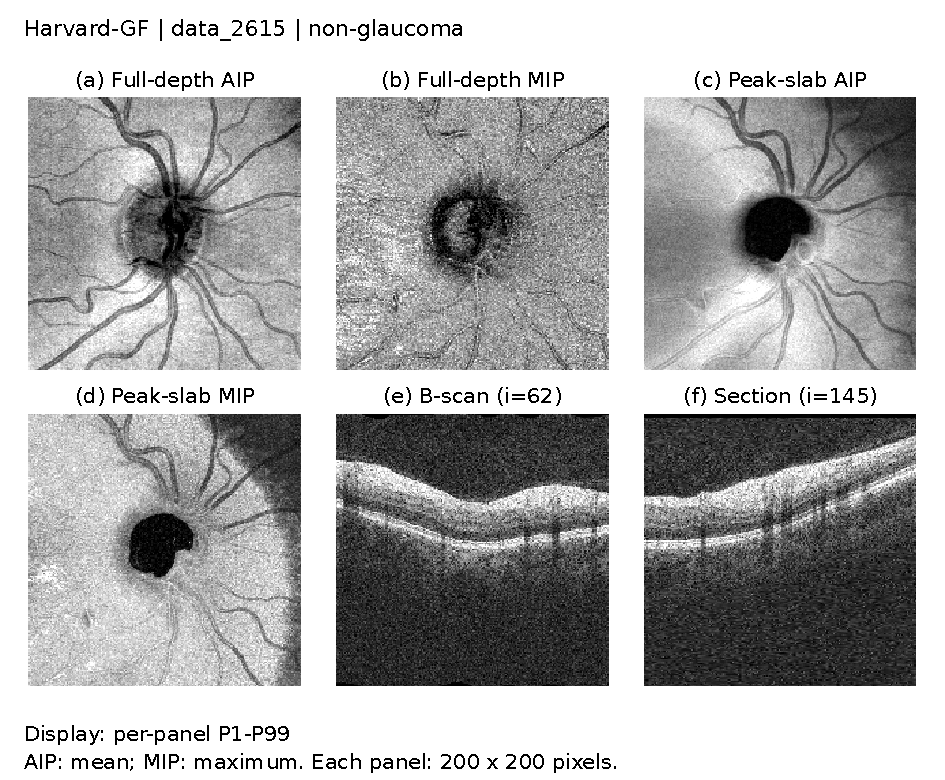
\includegraphics[width=\textwidth]{figures/projection_thesis/report_views_2615_thesis.pdf}
  \caption[Các ảnh chiếu và lát cắt từ thể tích OCT data\_2615]{%
    Các ảnh chiếu và lát cắt từ thể tích OCT thô \texttt{data\_2615}:
    (a,b) AIP và MIP toàn chiều sâu; (c,d) AIP và MIP trong dải
    quanh đỉnh cường độ; (e) B-scan; (f) lát cắt trực giao.}
  \label{fig:group-a-inputs}
\end{figure}

Trong hình, trục chiều sâu là trục nguồn 1; dải chiếu gồm các
chỉ số 47--79, lấy cả hai đầu, với tâm tại chỉ số 63. B-scan
ở trục nguồn 2, chỉ số 62; lát cắt trực giao ở trục nguồn 0,
chỉ số 145. Các trục và chỉ số nguồn được đếm từ 0. Hai lát cắt
được chọn theo độ lệch chuẩn lớn nhất sau giới hạn P1/P99 trong
khoảng chỉ số 30--169, không nhất thiết là lát trung tâm hay
đại diện lâm sàng. Mỗi ô giữ đủ $200\times200$ pixel và dùng
giới hạn hiển thị P1/P99 riêng, nên độ sáng giữa các ô không có
cơ sở so sánh trực tiếp. Tỷ lệ pixel trong hình là tỷ lệ theo mảng,
không phải tỷ lệ vật lý đã hiệu chuẩn; dải quanh đỉnh cũng
không đồng nhất với lớp RNFL được phân đoạn.
\FloatBarrier

\subsection{Bộ trích xuất đặc trưng ảnh chiếu 2D MaxViT}
\label{sec:maxvit-method}
\subsubsection{Cơ chế tích chập và chú ý đa trục}
MaxViT kết hợp MBConv, block attention và grid attention trong các
khối phân cấp \cite{tu2022maxvit}. Với bản đồ đặc trưng $F$, lược đồ là
\begin{equation}
 F'=\mathcal A_G\!\left(\mathcal A_B(\mathcal M(F))\right),
 \label{eq:maxvit-block}
\end{equation}
trong đó $\mathcal M$ là MBConv, $\mathcal A_B$ và $\mathcal A_G$ là
hai khối attention. MBConv gồm phép chiếu kênh $1\times1$, tích chập
riêng từng kênh và điều biến kênh SE. Block attention nhóm token trong
cửa sổ liền kề; grid attention nhóm các vị trí cách đều trên bản đồ,
tạo tương tác xa mà không dùng attention dày trên toàn ảnh ở mỗi lớp.

Hình~\ref{fig:maxvit-architecture} thể hiện kiến trúc phân cấp và cấu
trúc bên trong một khối MaxViT. Các tầng tích chập đầu mạng tạo bản đồ
đặc trưng, sau đó các khối MaxViT được lặp qua bốn giai đoạn với độ
phân giải giảm dần. Phần đầu phân loại trong sơ đồ là của mạng gốc;
trong nhánh ảnh chiếu, đặc trưng trước tầng phân loại được sử dụng
cho phép hợp nhất.

\begin{figure}[htbp]
 \centering
 % Trích Hình 2, trang 5 từ prism-uploads/2204.01697v4.pdf; giữ nguyên nội dung sơ đồ.
 \includegraphics[width=\textwidth]{figures/methods/maxvit-tu-2022-fig2.png}
 \caption[Kiến trúc tổng thể và khối cơ bản của MaxViT]{Kiến trúc tổng
 thể và khối cơ bản của MaxViT, kết hợp MBConv, block attention và grid
 attention. Nguồn: trích Hình~2, tr.~5 của Tu và cộng sự (2022), bản
 arXiv:2204.01697v4 \cite{tu2022maxvit}.}
 \label{fig:maxvit-architecture}
\end{figure}
\FloatBarrier

Với nhóm token $U\in\mathbb R^{m\times d}$, một đầu chú ý có dạng:
\begingroup
\setlength{\jot}{8pt}
\begin{align}
 Q_h&=UW_h^Q,\quad K_h=UW_h^K,\quad V_h=UW_h^V,\\
 A_h(U)&=\operatorname{softmax}\!\left(
 \frac{Q_hK_h^\top}{\sqrt{d_h}}+B_h\right)V_h,\\
 \operatorname{MSA}(U)&=[A_1(U);\ldots;A_H(U)]W^O.
 \label{eq:maxvit-attention}
\end{align}
\endgroup
$d_h$ là chiều khóa, $B_h$ là độ lệch vị trí tương đối học được;
softmax tính theo token khóa. Các đầu chú ý được nối theo chiều đặc
trưng. Nhánh dư và mạng truyền thẳng trong khối có thể viết:
\begin{align}
 U'&=U+\operatorname{MSA}(\operatorname{LN}(U)),\\
 U''&=U'+\operatorname{FFN}(\operatorname{LN}(U')).
 \label{eq:maxvit-residual}
\end{align}
LN là chuẩn hóa lớp; FFN là mạng truyền thẳng theo kênh. Đặc trưng
trước tầng logits là đầu ra của bộ trích xuất đặc trưng phục vụ phép hợp nhất.

\subsubsection{Lựa chọn từ khảo sát và phạm vi triển khai}
Trên tập kiểm tra, MaxViT đạt AUROC 0,7638, PR-AUC 0,7925 và MCC 0,3765,
cao nhất trong sáu lần chạy 2D. Tuy nhiên, F1 0,7065 thấp hơn Tiny2D-SlabMIP 0,7195;
ECE 0,1265 và thời gian chạy 37,95 phút cũng chưa thuận lợi nhất.
Các kết quả hỗ trợ ưu tiên MaxViT về khả năng phân biệt, không chứng
minh ưu thế trên mọi tiêu chí hoặc độ ổn định giữa các lần chạy.

Biến thể được triển khai là \texttt{maxvit\_tiny\_rw\_224}; ảnh chiếu có
kích thước $224\times224$. Khảo sát đơn nhánh nêu trên sử dụng trọng số
tiền huấn luyện trên ImageNet và đầu vào Slab AIP, nên các chỉ số đó
không phải kết quả đo riêng cho hai nhánh Slab MIP và AIP toàn khối.
Trong \texttt{FinalModel}, hai bộ trích xuất được khởi tạo riêng trong
\texttt{ModuleList}, không chia sẻ tham số. Mỗi bộ bỏ đầu phân loại
(\texttt{num\_classes=0}), gộp trung bình toàn cục và trả vector 512 chiều.
Mã ưu tiên đầu vào một kênh qua \texttt{in\_chans=1}; nếu bước tạo mô hình
này phát sinh ngoại lệ, nhánh dự phòng tạo mô hình mặc định và lặp ảnh
xám thành ba kênh. Vì vậy, nhánh khởi tạo thực sự sử dụng và phiên bản
\texttt{timm} cần được lưu cùng cấu hình chạy.
Lượt warm-start cuối nạp trọng số từ checkpoint raw đã xác minh, thay
vì coi trọng số tiền huấn luyện ImageNet là trạng thái khởi đầu trực tiếp.



\subsection{Bộ trích xuất đặc trưng khối OCT ResNeXt3D}
\label{sec:resnext3d-method}
\subsubsection{Khối dư tổng hợp và tích chập nhóm}
ResNeXt tổng hợp nhiều phép biến đổi cùng cấu trúc trong một khối dư
\cite{xie2017resnext}:
\begin{equation}
 Y=S(X)+\sum_{c=1}^{C_g}\mathcal T_c(X).
 \label{eq:resnext-aggregate}
\end{equation}
$S$ là đường tắt đồng nhất hoặc phép chiếu; $C_g$, gọi là cardinality,
là số phép biến đổi, không phải số nhánh ảnh trong mô hình hợp nhất đặc trưng.

Hình~\ref{fig:resnext-equivalent-blocks} minh họa mối liên hệ giữa
phép tổng hợp nhiều đường biến đổi và cách cài đặt bằng tích chập
nhóm. Ba sơ đồ biểu diễn các khối tương đương trong kiến trúc 2D:
phép cộng đầu ra các đường biến đổi có thể được tổ chức lại thành
phép nối đặc trưng và phép chiếu kênh, rồi biểu diễn gọn bằng tích
chập nhóm. Các số kênh và số nhóm trong hình là cấu hình minh họa
của nguồn, không phải đặc tả nhánh OCT của luận văn.

\begin{figure}[htbp]
 \centering
 % Trích Hình 3, trang 4 từ prism-uploads/1611.05431v2.pdf; giữ đủ ba phần.
 \includegraphics[width=\textwidth]{figures/methods/resnext-xie-2017-fig3.png}
 \caption[Các cách biểu diễn tương đương của khối ResNeXt 2D]{Các cách
 biểu diễn tương đương của khối ResNeXt 2D: (a) tổng hợp các biến đổi
 dư; (b) nối đặc trưng trước phép chiếu; (c) tích chập nhóm. Nguồn:
 trích Hình~3, tr.~4 của bản arXiv:1611.05431v2, Xie và cộng sự
 \cite{xie2017resnext}.}
 \label{fig:resnext-equivalent-blocks}
\end{figure}
\FloatBarrier

Bài báo gốc trình bày mạng 2D. Trong nhánh 3D hiện tại, bottleneck
theo nhóm được triển khai bằng chuỗi toán tử:
\begingroup
\setlength{\jot}{8pt}
\begin{align}
 X_1&=\phi(\operatorname{GN}_1(\operatorname{Conv}^{\mathrm{in}}_{1\times1\times1}(X))),\\
 X_2&=\phi(\operatorname{GN}_2(\operatorname{GConv}_{3\times3\times3,C_g}(X_1))),\\
 \mathcal F_3(X)&=\operatorname{Conv}^{\mathrm{out}}_{1\times1\times1}(X_2).
 \label{eq:resnext3d-bottleneck}
\end{align}
\endgroup
Ở đây, $\phi=\operatorname{ReLU}$, GN là GroupNorm và đầu ra khối là
$\phi(S(X)+\mathcal F_3(X))$. Nếu số kênh hoặc stride thay đổi, $S$
gồm tích chập $1\times1\times1$ và GroupNorm; nếu không, $S$ là ánh xạ
đồng nhất. Thuộc tính \texttt{g3} được khai báo trong mã nhưng không
được gọi trong \texttt{forward}; do đó không có GroupNorm sau phép
chiếu cuối của nhánh dư trong biểu thức trên. Tích chập theo nhóm chỉ nối
mỗi kênh ra với các kênh vào cùng nhóm. Với $C_b$ kênh vào/ra chia đều
thành $C_g$ nhóm, kernel $3^3$ có $27C_b^2/C_g$ trọng số, chưa tính bias,
so với $27C_b^2$ khi không chia nhóm; tỷ lệ này không đại diện cho toàn mạng.

Hình~\ref{fig:resnext3d-reference-block} thể hiện một khối ResNeXt
với tích chập 3D, làm rõ chuỗi phép chiếu $1\times1\times1$, tích
chập nhóm $3\times3\times3$ và kết nối dư
\cite{hara2018spatiotemporal}. Trong ký hiệu của hình, $F$ là số kênh
đặc trưng và BN là chuẩn hóa theo lô. Kiến trúc tham khảo được xây
dựng cho video; khi áp dụng cho khối OCT, chiều thứ ba biểu diễn
chiều không gian của khối ảnh, không phải thời gian. Giá trị
$\mathrm{group}=32$ thuộc cấu hình trong nguồn và không được mặc
định là số nhóm của mô hình đang khảo sát.

\begin{figure}[htbp]
 \centering
 % Cắt riêng cột ResNeXt từ Hình 3, trang PDF thứ 4 của prism-uploads/document.pdf.
 \includegraphics[height=6.8cm]{figures/methods/resnext3d-hara-2018-fig3-detail.png}
 \caption[Khối ResNeXt sử dụng tích chập 3D]{Khối ResNeXt sử dụng tích
 chập 3D. Nguồn: trích riêng phần ResNeXt trong Hình~3 của Hara và
 cộng sự (2018) \cite{hara2018spatiotemporal}.}
 \label{fig:resnext3d-reference-block}
\end{figure}
\FloatBarrier

Bản đồ cuối được gộp trung bình theo ba chiều không gian:
\begin{equation}
 [e_{3D}]_c=\frac{1}{D'H'W'}\sum_{d=1}^{D'}\sum_{h=1}^{H'}
 \sum_{w=1}^{W'}[F_3]_{c,d,h,w}.
 \label{eq:resnext3d-embedding}
\end{equation}
Vector $e_{3D}$ là đầu ra của nhánh khối ảnh trước tầng phân loại.

\subsubsection{Căn cứ lựa chọn và cấu hình triển khai}
Lần chạy \texttt{single3d-resxt3d} đạt AUROC trên tập kiểm tra 0,8538, PR-AUC 0,8798 và
F1 0,7836, cao nhất trong bảng khảo sát 3D mở rộng. MCC 0,542 đồng hạng
với VNet sau làm tròn; độ chính xác (accuracy) 0,7711 thấp hơn 0,7744 của
\texttt{denoise-enc-32-d5}, nhưng hai lần chạy sử dụng quy trình khác nhau. Vì vậy,
ResNeXt3D được chọn cho nhánh 3D; VNet và SegResNet chỉ thuộc khảo sát đã có,
không được bổ sung vào kế hoạch huấn luyện cuối.
Chưa có căn cứ kết luận ưu thế có ý nghĩa thống kê.

Lần chạy khảo sát tham chiếu sử dụng $96^3$ và 15 epoch, trong khi nhánh
ResNeXt3D của mô hình đề xuất nhận trực tiếp khối $200^3$ sau tiền xử
lý. Các chỉ số của lần chạy khảo sát không phải kết quả đã đo cho cấu hình
$200^3$ này. Mã hiện tại dùng stem tích chập $3^3$, stride 1, padding 1,
với 32 kênh, GroupNorm và ReLU. Bốn mức kênh là $(32,64,128,192)$;
mức đầu có một khối dư giữ nguyên kích thước, mỗi mức sau có một khối
chuyển mức và một khối stride 1, tổng cộng bảy khối dư. Tích chập nhóm
có $C_g=8$, \texttt{base\_width=8}, nên bề rộng bottleneck bằng số kênh
đầu ra tại các mức này. GroupNorm sử dụng 8 nhóm.

Ba khối chuyển mức thực sự dùng stride $(2,2,2)$, tạo chuỗi kích thước
$200^3\to100^3\to50^3\to25^3$. Phần tử stride $(2,2,1)$ đầu tiên
trong danh sách cấu hình không được sử dụng, do mã chỉ tạo khối chuyển
mức khi chỉ số mức lớn hơn 0. Vì vậy, không mô tả nhánh này như một
mạng giảm mẫu bất đẳng hướng bảo toàn riêng trục chiều sâu.
\texttt{AdaptiveAvgPool3d(1)} ở cuối tạo vector $e_{3D}$ 192 chiều.
Đây là cấu hình ResNeXt3D tùy biến, không được đồng nhất với
ResNeXt-50/101 hoặc $32\times4d$. Bộ khởi tạo không nạp trọng số tiền
huấn luyện 3D; trong lượt cuối, trạng thái nhánh này cũng được lấy từ
checkpoint raw đã xác minh.



\section{Cơ chế tích hợp và kết nối}
\label{sec:integration}
\subsection{Tương ứng dữ liệu giữa các nhánh}
Trong mã hiện tại, mỗi mẫu gồm một khối 3D, hai ảnh chiếu 2D và một
nhãn tham chiếu, được trả về dưới dạng bộ ba \texttt{(x, views, labels)}.
Khối, ảnh chiếu và nhãn được ghép theo cùng chỉ số trong các mảng;
mã nạp dữ liệu không thực hiện phép nối theo ID bệnh nhân. Vì vậy,
sự tương ứng về thứ tự mẫu và tính độc lập theo bệnh nhân của phân
hoạch cần được xác minh từ dữ liệu nguồn, không suy ra từ giao diện này.
Hàm \texttt{aug\_pair} áp dụng chung các phép lật, xoay góc bội của
$90^\circ$ và biến đổi cường độ cho khối cùng hai ảnh chiếu. Mã hiện tại
xác định ngẫu nhiên tăng cường theo seed, epoch và chỉ số mẫu, với
\texttt{num\_workers=0}. Lọc và tạo ảnh chiếu không có tham số học.

\texttt{FinalDataset} hiện tại tạo cache ảnh chiếu từ đúng tệp khối
được chọn. Khi chọn dữ liệu sau khử nhiễu, cả khối 3D, trục suy đoán
và hai ảnh chiếu đều có nguồn từ dữ liệu đó. Ngược lại, notebook cũ
tạo cache ảnh chiếu từ khối raw và dùng chung cache cho cả lựa chọn
raw lẫn denoised; ở lựa chọn denoised cũ, chỉ nguồn khối 3D thay đổi.
Sửa đổi cache theo nguồn dữ liệu không có hiệu lực hồi tố đối với
lần chạy \texttt{raw\_s42} hoặc phiên notebook cũ đang thực thi.

\subsection{Giao diện đặc trưng và phép chiếu}
\label{sec:branch-backbones}
Gọi $e_0=f_{\mathrm{ResNeXt3D}}(X_3)$ và
$e_i=f_{\mathrm{MaxViT},\theta_i}(U_i)$, $i=1,2$, là đặc trưng
trước tầng phân loại của từng nhánh, với $X_3=X_{3D}$,
$U_i=X_{2D}^{(i)}$, $d_0=192$ và $d_1=d_2=512$.
Hai bộ tham số $\theta_1,\theta_2$ độc lập. Các vector
được đưa về cùng chiều $d_f=256$ bằng phép chiếu học được:
\begin{equation}
 p_i=\operatorname{ReLU}(W_i e_i+b_i)\in\mathbb R^{256},\qquad i=0,1,2.
 \label{eq:group-a-proj}
\end{equation}
Với lô dữ liệu $N$ mẫu, đầu ra nhánh $i$ có dạng $N\times d_i$;
$W_i\in\mathbb R^{d_f\times d_i}$ và $b_i\in\mathbb R^{d_f}$.
Phép chiếu giải quyết khác biệt số chiều giữa các bộ trích xuất đặc trưng,
thay vì nối trực tiếp tensor ảnh 2D với tensor khối 3D. Mỗi nhánh có
một lớp Linear và ReLU riêng; không có lớp chuẩn hóa trong phép chiếu này.
Quy ước $p_0$ luôn chỉ nhánh 3D, còn $p_1,p_2$ lần lượt chỉ Slab MIP
và AIP toàn khối, tránh nhầm chỉ số nhánh với số chiều không gian.

\subsection{Hợp nhất đặc trưng 2D--3D bằng CrossGate}
\label{sec:crossgate-fusion}
CrossGate là cơ chế hợp nhất đặc trưng được chọn cho mô hình đề xuất. Nhánh
3D cung cấp đặc trưng nền để phân loại, còn các đặc trưng ảnh chiếu
2D bổ sung thông tin thông qua chú ý chéo. Theo sơ đồ tại
Hình~\ref{fig:crossgate-module}, đặc trưng 3D được dùng làm truy vấn
($Q$); các đặc trưng 2D được chuẩn hóa lớp (LayerNorm) trước khi
đưa vào vai trò khóa và giá trị ($K,V$). Đầu ra chú ý được nhân
với cổng vô hướng rồi cộng vào đặc trưng 3D.

Với ký hiệu phép chiếu ở Phương trình~\eqref{eq:group-a-proj}, đặt
\begin{equation}
 P_{3D}=p_0^{\mathsf T}\in\mathbb R^{1\times d_f},\qquad
 T_{2D}=\begin{bmatrix}p_1^{\mathsf T}\\p_2^{\mathsf T}\end{bmatrix}
 \in\mathbb R^{2\times d_f}.
 \label{eq:crossgate-inputs}
\end{equation}
Mỗi ảnh chiếu tạo một token trong $T_{2D}$. Với lô dữ liệu $N$ mẫu,
các tensor tương ứng có dạng $N\times1\times d_f$ và
$N\times2\times d_f$. Tổng cộng có ba token sau phép chiếu, nhưng chỉ
hai token 2D cung cấp khóa và giá trị cho một truy vấn 3D.
Trong hình tham khảo, ký hiệu $p_3$ chỉ đặc trưng nhánh 3D,
tương ứng với $P_{3D}=p_0^{\mathsf T}$ ở đây; mô hình hiện tại không
có nhánh ảnh chiếu thứ ba. Số token và kích thước triển khai được
quy định bởi Phương trình~\eqref{eq:crossgate-inputs}.

Phép kết hợp cho mỗi mẫu được viết gọn thành
\begin{align}
 \widetilde T_{2D}&=\operatorname{LN}(T_{2D}),\\
 o&=\operatorname{MHA}(P_{3D},\widetilde T_{2D},\widetilde T_{2D}),\\
 z&=P_{3D}+\sigma(\alpha)\,o.
 \label{eq:crossgate-fusion}
\end{align}
Ba đối số của MHA lần lượt là đầu vào truy vấn, khóa và giá trị;
các phép chiếu học được nằm trong khối chú ý. Mã hiện tại sử dụng
8 đầu chú ý, mỗi đầu 32 chiều, và dropout 0,1 trên trọng số chú ý
trong huấn luyện. LayerNorm chỉ áp dụng cho token khóa và giá trị,
không áp dụng cho truy vấn 3D. Hàm $\sigma$ là sigmoid, đưa tham
số cổng $\alpha$ về khoảng $(0,1)$ để điều chỉnh mức đóng góp của
đầu ra chú ý. Cổng vô hướng điều tiết toàn bộ vector bổ sung,
không phải cổng riêng cho từng kênh. Đường tắt
giữ lại đặc trưng 3D, còn $z$ được đưa tới đầu phân loại.

\begin{figure}[htbp]
 \centering
 % Bản PDF vector do tác giả cung cấp; cắt lề trắng và nhãn (b) của hình rời.
  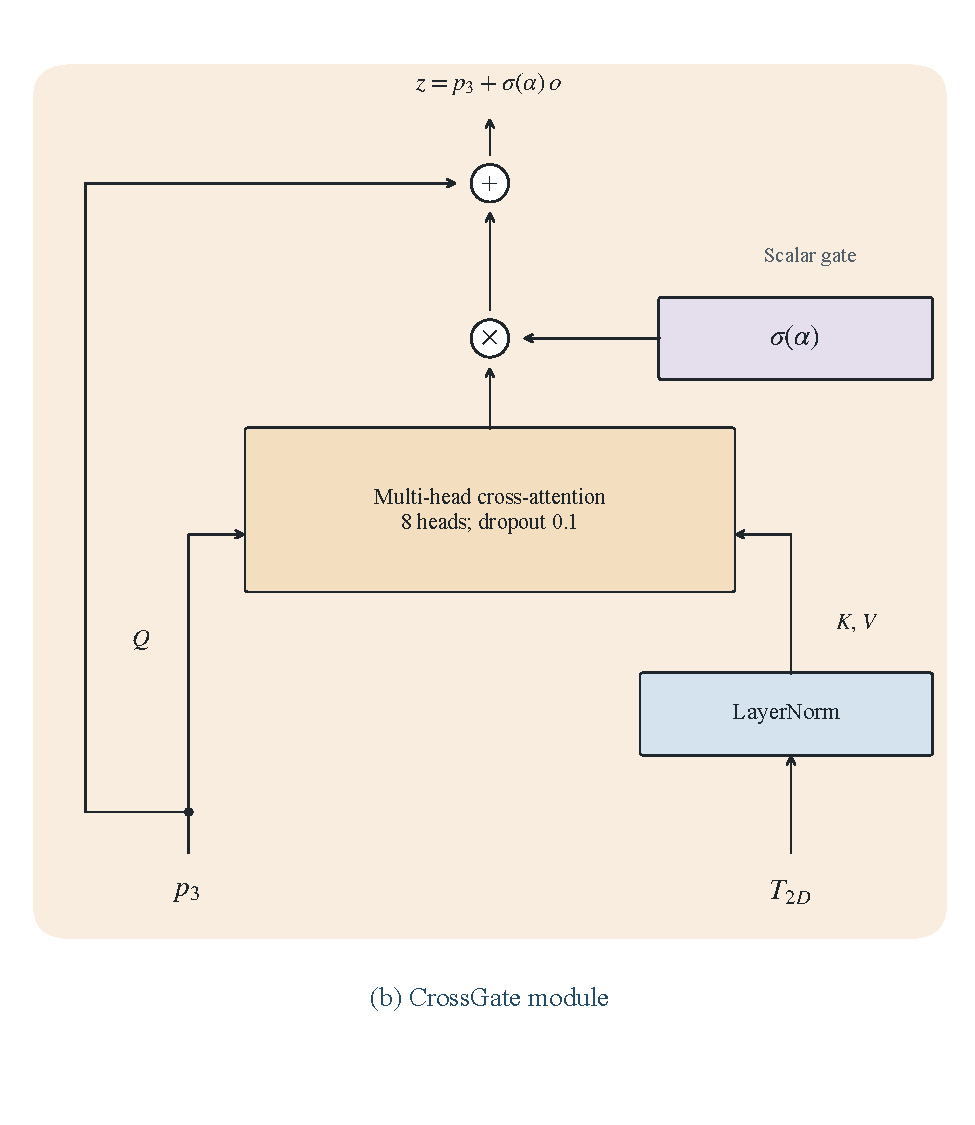
\includegraphics[trim=10bp 80bp 10bp 25bp,clip,width=\textwidth]{figures/architecture_publication/02_crossgate.pdf}
 \caption[Cơ chế CrossGate kết hợp đặc trưng 2D--3D]{Cơ chế CrossGate
 kết hợp đặc trưng 2D--3D: nhánh 3D tạo truy vấn, các token 2D
 sau LayerNorm cung cấp khóa và giá trị; đầu ra chú ý được nhân
 với cổng vô hướng rồi cộng vào đặc trưng 3D.}
 \label{fig:crossgate-module}
\end{figure}
\FloatBarrier

Tham số vô hướng $\alpha$ được khởi tạo bằng $0{,}5$, nên hệ số
cổng ban đầu là $\sigma(0{,}5)\approx0{,}6225$, không phải $0{,}5$.
Trong lượt warm-start, giá trị cổng được nạp từ checkpoint cùng các
trọng số khác; giá trị sau huấn luyện không được suy ra từ giá trị
khởi tạo. Đặc trưng hợp nhất được đưa trực tiếp qua một lớp Linear
$256\to2$, không có tầng ẩn bổ sung. Đặc tả này xác nhận luồng tính
toán, không tự nó chứng minh lợi ích phân loại của CrossGate.

% ===== TẠM ẨN: giữ nguyên nội dung, bỏ tiền tố comment để khôi phục =====
% , với công thức và suy dẫn gradient tại Mục~\ref{sec:attention-theory}.
% ===== HẾT NỘI DUNG TẠM ẨN; đoạn thay thế đang hiển thị bên dưới =====
% ===== KẾT THÚC KHỐI TẠM ẨN =====
% ===== TẠM ẨN: giữ nguyên nội dung, bỏ tiền tố comment để khôi phục =====
% \subsection{Chi phí dự kiến và giới hạn của giả thuyết}
% Theo ước lượng thiết kế, \texttt{Enc3D} có khoảng 2,0 triệu tham số, mỗi
% \texttt{Enc2D} khoảng 11,2 triệu và mô hình hợp nhất khoảng 36,5 triệu.
% Các số liệu này chưa được kiểm đếm độc lập từ mã nguồn. Tổng số tham
% số phụ thuộc từng phép hợp nhất do khác biệt ở đầu phân loại và khối
% attention. Ba bộ trích xuất đặc trưng 2D đóng góp khoảng
% 33,6 triệu tham số, lớn hơn đáng kể so với nhánh
% 3D 2,0 triệu. VRAM và thời gian mỗi epoch vẫn chưa có số đo.
%
% Giả thuyết cần kiểm tra là fusion cải thiện hiệu năng so với
% \texttt{single3d} trong cùng điều kiện đánh giá, với mức chi phí có thể chấp
% nhận. Nếu có cải thiện, vẫn phải xét ảnh hưởng của số tham số, dung lượng
% đầu phân loại và sai số chọn mô hình; không mặc định quy toàn bộ cải thiện
% cho phép chiếu hoặc attention. Nếu không cải thiện, cần báo cáo trung thực
% và phân tích khả năng chọn sai trục/dải, mất thông tin khi chiếu hoặc tối ưu
% chưa phù hợp. Bảng~\ref{tab:group-a-pending} dành cho kết quả sẽ bổ sung sau.
% ===== KẾT THÚC KHỐI TẠM ẨN =====
\subsection{Đầu phân loại và giao diện đầu ra}
Trong biểu diễn cho một mẫu, chiều token đơn được lược bỏ khi viết
đặc trưng dưới dạng vector. Cụ thể, mã nguồn gọi \texttt{squeeze} trên
đầu ra chú ý trước phép cộng dư, nên $z$ truyền tới đầu phân loại
không còn chiều token đơn. Với
$a=g_{\theta_h}(z)\in\mathbb R^2$ là logits của hai lớp, điểm số
và nhãn dự đoán được xác định bởi
\begin{equation}
 \widehat p=\frac{\exp(a_1)}{\exp(a_0)+\exp(a_1)},\qquad
 \widehat y=\boldsymbol{1}\{\widehat p\geq\tau\}.
 \label{eq:integration-output}
\end{equation}
Trong mã hiện tại, bộ tối ưu nhận toàn bộ tham số mô hình; không có
chính sách đóng băng riêng các bộ trích xuất đặc trưng trong huấn luyện.
Đầu phân loại trả logits thô cho cross-entropy có trọng số lớp, không
áp dụng sigmoid trước hàm mất mát. Phương trình~\eqref{eq:integration-output}
mô tả điểm số chưa hiệu chuẩn; bước đánh giá cuối dùng thêm nhiệt độ
được khớp trên tập xác thực. Hàm mất mát cross-entropy được trình bày
tại Mục~\ref{sec:evaluation-metrics}.

Với lô $N$ mẫu, giao diện mạng nhận tensor khối
$N\times1\times200\times200\times200$ và tensor ảnh chiếu
$N\times2\times1\times224\times224$, rồi trả logits $N\times2$.
Nhãn tham chiếu có dạng $N$ phần tử, được dùng bởi hàm mất mát nhưng
không phải đầu vào của phép suy luận. Các bước hiệu chuẩn và chọn
ngưỡng nằm ngoài mạng; chúng không làm thay đổi giao diện logits này.

\section{Chiến lược huấn luyện}
\subsection{Hai giai đoạn và giới hạn huấn luyện}
Chiến lược cuối gồm một giai đoạn raw đã có bằng chứng quan sát và
một giai đoạn huấn luyện tiếp trên dữ liệu khử nhiễu còn dự kiến:
\begin{enumerate}[label=\arabic*.,leftmargin=1cm]
 \item Giai đoạn raw: nhật ký \texttt{raw\_s42} ghi nhận epoch 1--22
 trong ngân sách danh nghĩa 30 epoch. Đây là bằng chứng huấn luyện
 và xác thực theo notebook cũ, không xác nhận đã hoàn tất 30 epoch,
 nguyên nhân kết thúc nhật ký hoặc kết quả kiểm tra.
 Mục~\ref{sec:raw-s42-results} trình bày các chỉ số và giới hạn của nguồn này.
 \item Giai đoạn denoised: chỉ thực hiện một lượt warm-start 10 epoch
 trên dữ liệu Bilateral, sau khi xác minh checkpoint raw tương thích.
 Sau lượt này, cố định trọng số mạng để đánh giá, hậu xử lý và phân
 tích khả năng giải thích (XAI); không thêm mô hình, seed, lượt raw
 đối chứng hoặc huấn luyện ablation.
\end{enumerate}
Mục~\ref{sec:final-denoise-plan} quy định giao thức thực hiện chi tiết.
Hai giai đoạn không tạo thành một phép đối chứng riêng cho khử nhiễu,
vì giai đoạn sau đồng thời thay nguồn đầu vào và cập nhật thêm trọng số.
Notebook hiện vẫn có mặc định 30 epoch, danh sách raw/Bilateral, ba seed
và patience 6; các mặc định này không phải giao thức cuối đã chốt.
Cấu hình thực thi phải giới hạn đúng một lượt denoised 10 epoch;
trạng thái kết thúc và số epoch thực hoàn tất phải được báo cáo.

\subsection{Hàm mục tiêu và cơ chế tối ưu}
Phiên bản notebook hiện tại sử dụng \texttt{Trainer} trong
\texttt{scripts/final\_training.py}: AdamW, tốc độ học mặc định
$2\times10^{-4}$, weight decay $10^{-4}$, micro-batch 2 và tích lũy
8 micro-batch. Một cửa sổ đầy đủ tương ứng 16 mẫu; cửa sổ cuối có thể
nhỏ hơn. Lịch học gồm warmup trong 5\% số bước dự kiến rồi suy giảm
cosine, kết hợp AMP float16 trên CUDA và chặn chuẩn gradient ở mức 1.
Checkpoint tốt nhất được chọn theo AUROC xác thực. Các mặc định này
mô tả mã hiện tại, không thay thế cấu hình thực chạy cần lưu trong
nhật ký và không được gán hồi tố cho \texttt{raw\_s42}.

Trọng số của lớp $c$ được tính bởi $w_c=N_{\mathrm{train}}/(2N_c)$
trên tập huấn luyện, trong đó $N_{\mathrm{train}}$ là tổng số mẫu và $N_c$ là số
mẫu thuộc lớp $c$. Đặt $\ell_j=-\log q_{j,y_j}$, trong đó $q_{j,y_j}$
là xác suất softmax chưa hiệu chuẩn gán cho lớp thật $y_j$ của mẫu $j$.
Giá trị loss ghi nhận cho một epoch trong
\texttt{Trainer} hiện tại là
\begin{equation}
 L_{\mathrm{current}}=
 \frac{\sum_{j\in\mathcal E}w_{y_j}\ell_j}{\sum_{j\in\mathcal E}w_{y_j}},
\end{equation}
trong đó $\mathcal E$ là tập mẫu đã xử lý trong epoch. Log theo bước
dùng cùng tỷ số trên phần epoch đã xử lý. Gradient được cộng theo
tử số rồi chia cho tổng trọng số mẫu của từng cửa sổ tích lũy, kể cả
cửa sổ cuối không đầy đủ.

\subsection{Phân biệt nhật ký hiện tại và lịch sử}
Ngược lại, phiên bản notebook cũ tại Git HEAD khi đối chiếu dùng loss trung bình có trọng số
của từng micro-batch, chia tiếp cho hệ số tích lũy $G$ trước khi cộng
vào bộ đếm; giá trị mặc định trong mã cũ là $G=8$.
Với $M$ micro-batch, giá trị in ra là
\begin{equation}
 L_{\mathrm{legacy}}=\frac{1}{MG}\sum_{b=1}^{M}
 \frac{\sum_{j\in\mathcal B_b}w_{y_j}\ell_j}
      {\sum_{j\in\mathcal B_b}w_{y_j}}.
\end{equation}
Do đó, loss xấp xỉ $0{,}08$ trong dòng
\texttt{[raw\_s42] ep x/30 loss=...}, kèm các trường
\texttt{val\_auc}, \texttt{val\_bal} và \texttt{mcc},
không phải loss theo định nghĩa hiện tại. Nếu xác nhận cấu hình thực
chạy có $G=8$, nhân giá trị cũ với 8 chỉ khôi phục trung bình loss của
các micro-batch, không nhất thiết bằng tỷ số tổng trọng số trên toàn
epoch. Luận văn giữ nguyên loss lịch sử, không tự quy đổi khi cấu hình
thực chạy chưa được xác minh độc lập. Định dạng dòng này khớp notebook
cũ; \texttt{Trainer} mới in một từ điển lịch sử. Các chỉ số xác thực
phụ thuộc ngưỡng trong log cũ dùng xác suất chưa hiệu chuẩn và ngưỡng
$0{,}5$; AUROC được tính từ điểm số, không phụ thuộc ngưỡng đó.
Phần diễn giải bằng chứng lịch sử nằm tại Mục~\ref{sec:raw-s42-results}.

\subsection{Khởi tạo trọng số và khả năng tái lập}
Warm-start chỉ nạp trọng số, không phải khôi phục chính xác phiên
huấn luyện: optimizer, scheduler, GradScaler, epoch, lịch sử và danh
tính W\&B bắt đầu lại. Trước lượt cuối cần xác minh tệp trọng số thực
sự tồn tại, nguồn gốc raw và khả năng nạp nghiêm ngặt vào đúng kiến
trúc. Không suy ra đường dẫn, epoch nguồn hoặc tính sẵn có của
checkpoint chỉ từ một dòng log. Cơ chế resume đầy đủ của mã mới lưu
thêm trạng thái tối ưu, ngẫu nhiên, thứ tự mẫu và vị trí xử lý tại
ranh giới cửa sổ tích lũy đã hoàn tất; cơ chế đó không phục hồi các
trạng thái không được lưu trong lần chạy cũ.

Nhật ký của lượt cuối cần ghi phiên bản mã, cấu hình, ID lần chạy,
nguồn checkpoint, trạng thái kết thúc và định nghĩa chỉ số. Mã hiện
tại yêu cầu ghi W\&B và đồng bộ sản phẩm lên Drive cho lượt chạy thật;
đây là đặc tính triển khai, không phải xác nhận rằng sản phẩm của một
lượt cụ thể đã được lưu thành công. Cấu hình và kết quả của các khảo
sát đã thực hiện được trình bày riêng tại các phụ lục tương ứng.

% ===== TẠM ẨN: giữ nguyên nội dung, bỏ tiền tố comment để khôi phục =====
% \label{sec:compute-plan}
%
% \subsection{Vai trò của các nền tảng và tiêu chí lựa chọn}
% Kế hoạch triển khai phân công máy cá nhân cho phát triển mã, kiểm tra
% luồng xử lý và sinh hình báo cáo; máy có GPU phục vụ huấn luyện Nhóm A.
% Theo ghi nhận của tác giả, môi trường cá nhân hiện dùng PyTorch CPU và
% đã chạy smoke test. Đây là thông tin nhật ký, chưa được kiểm chứng bằng
% log trong luận văn. Smoke test chỉ kiểm tra những đường chạy đã thực
% thi, không bảo đảm hết lỗi, đủ VRAM hoặc đúng kết quả ở độ phân giải thật.
% Không quy đổi việc không thuê GPU thành tổng chi phí vận hành bằng không.
%
% Google Colab là một phương án chạy notebook; tài nguyên và thời lượng
% phiên phụ thuộc gói dịch vụ, mức sử dụng và khả năng cấp phát, không có
% bảo đảm mọi phiên đều kéo dài một khoảng cố định \cite{colabFAQ}.
% Vast.ai là phương án thuê tài nguyên với mức phí phụ thuộc từng máy;
% ngoài thời gian thuê còn có thành phần lưu trữ và truyền dữ liệu
% \cite{vastBilling}. Luận văn không khẳng định một nền tảng luôn rẻ nhất
% hoặc Colab luôn đắt hơn theo một tỷ lệ cố định.
%
% Mục tiêu thử nghiệm ban đầu trong kế hoạch là một GPU A100 40~GB, nếu
% có sẵn và phù hợp ngân sách tại thời điểm thuê. Đây là lựa chọn để đo
% khả thi, không phải cấu hình đã được xác nhận chạy thành công. Khi so
% sánh với máy GPU khác hoặc Colab, cần xét đồng thời VRAM, tốc độ xử lý,
% CPU/RAM cho nạp dữ liệu, tốc độ đĩa/mạng, chính sách gián đoạn và tổng
% chi phí dự kiến. Không loại một GPU chỉ bằng tên thiết bị khi chưa có
% phép đo bộ nhớ cho đúng cấu hình.
%
% \subsection{Đo bộ nhớ và thời gian trước khi quét mô hình}
% Nhánh 3D có ít tham số hơn tổng ba nhánh 2D nhưng vẫn có thể tốn bộ nhớ
% do activation ở độ phân giải cao. Cần đo một cấu hình fusion đủ bốn
% nhánh ở $200^3$, với micro-batch 2, tám bước tích lũy và AMP, thay vì
% chỉ đo \texttt{single3d} rồi suy rộng cho toàn bộ mô hình. Kế hoạch dùng
% lượt chạy thử hai epoch để kiểm tra cả forward, backward, cập nhật
% optimizer, xác thực và ghi checkpoint. Thời gian khởi động/cache cần
% tách khỏi thời gian lặp ổn định; mỗi biến thể vẫn cần theo dõi VRAM cực đại.
%
% Nếu hết bộ nhớ, ưu tiên thử micro-batch 1 và 16 bước tích lũy để giữ
% batch hiệu dụng 16, đồng thời kiểm tra cách chuẩn hóa loss ở nhóm tích
% lũy cuối epoch. Tích lũy gradient không giảm bộ nhớ cần cho một lần
% forward/backward của micro-batch hiện tại. Nếu phải giảm kênh hoặc độ
% phân giải, cần đặt tên cấu hình mới và đánh giá lại các đối chứng; đó
% không còn là cùng kiến trúc ban đầu. AMP là lựa chọn tối ưu cần đo hiệu
% quả và kiểm tra tính hữu hạn của loss/gradient, không phải bảo đảm hết OOM.
%
% \subsection{Tổ chức dữ liệu, checkpoint và khôi phục phiên}
% Dữ liệu nên được tải và xác minh một lần trên cùng môi trường cho cả
% cụm thí nghiệm khi có thể. Cache dùng đường dẫn tương đối như
% \path{data/Training_volumes.npy}, kèm nhãn và manifest phân hoạch; kiểm
% tra số mẫu, mã bệnh nhân, checksum và phiên bản tiền xử lý trước khi
% tái sử dụng. Dung lượng 20--26~GB trong kế hoạch là ước lượng cần đo lại
% cho đúng phiên bản dữ liệu, không đồng nhất với mọi bộ Harvard đã nêu.
%
% Khảo sát đầy đủ bao gồm tám cấu hình tại Mục~\ref{sec:group-a}.
% Thứ tự thực hiện có thể ưu tiên \texttt{single3d}, fusion-concat
% và fusion-attention để phát hiện lỗi triển khai, sau đó mở rộng
% sang các cấu hình còn lại. Những lượt chưa thực hiện do giới hạn
% ngân sách được ghi nhận riêng; kết quả sơ bộ bất lợi không phải
% tiêu chí loại cấu hình khỏi kế hoạch đối chứng.
%
% Checkpoint tốt nhất phục vụ đánh giá, còn checkpoint gần nhất
% phục vụ khôi phục phiên huấn luyện. Checkpoint khôi phục bao gồm
% trọng số, optimizer, scheduler, trạng thái AMP nếu có, epoch/bước
% chạy, bộ đếm early stopping, trạng thái ngẫu nhiên và cấu hình.
% Nếu chỉ lưu ở cuối epoch, phần tính toán sau lần lưu gần nhất
% sẽ được thực hiện lại khi xảy ra gián đoạn. Khả năng khôi phục
% được kiểm tra trước các lượt huấn luyện dài trong kế hoạch triển khai.
%
% Phiên terminal độc lập như \texttt{tmux} giúp công việc không phụ thuộc
% kết nối SSH, nhưng không bảo vệ khi máy chủ bị thu hồi. Checkpoint và log
% cần được sao lưu định kỳ ra nơi lưu bền vững; mã thông báo truy cập không
% được ghi trong notebook, luận văn hoặc checkpoint. Sau khi xác nhận sao
% lưu thành công mới giải phóng tài nguyên thuê. Theo tài liệu Vast.ai,
% dừng instance không tự loại bỏ phí lưu trữ \cite{vastBilling}; mọi thao
% tác xóa tài nguyên phải đi sau kiểm tra dữ liệu đã lưu an toàn.
%
% \subsection{Mô hình dự toán và báo cáo chi phí}
% Đặt $E_r$ là số epoch thực chạy và $t_r$ là thời gian giây/epoch của cấu
% hình $r$, với phạm vi đo được định nghĩa nhất quán. Thời gian toàn quy
% trình dự kiến là
% \begin{equation}
%   T_{\mathrm{total}}=T_{\mathrm{setup}}+T_{\mathrm{probe}}+
%   \sum_{r=1}^{8}E_r t_r+T_{\mathrm{eval}}+T_{\mathrm{backup}}+T_{\mathrm{retry}}.
%   \label{eq:compute-total}
% \end{equation}
% Không cộng lặp thời gian đánh giá nếu nó đã nằm trong $t_r$. Giá thuê
% theo giờ $c_{\mathrm{GPU}}$ chỉ áp dụng cho thời gian thực sự tính phí;
% tổng tiền còn gồm lưu trữ, truyền dữ liệu và phí khác nếu có.
%
% Ví dụ kiểm tra phép tính, nếu giả định cả tám lượt đều chạy 15 epoch
% và mỗi epoch mất 60--150 giây, riêng tổng thời gian epoch là 2--5 giờ,
% chưa tính các thành phần còn lại. Đây không phải số đo tốc độ thực tế.
% Vì vậy, chưa dùng mức 5--15 USD hoặc 6--12 GPU-giờ trong ghi chú ban đầu
% làm kết quả đã xác nhận. Báo cáo cuối cần lưu ngày thuê, loại instance,
% mức giá thực tế, phạm vi đo thời gian, hóa đơn và chi phí cho từng cấu
% hình, cùng số seed đã chạy.
%
% ===== KẾT THÚC KHỐI TẠM ẨN =====
\subsection{Lựa chọn checkpoint và đánh giá với trọng số cố định}
Trong lượt huấn luyện cuối, checkpoint được lựa chọn theo AUROC xác
thực, không lựa chọn lại theo kết quả kiểm tra. Sau khi cố định trọng
số, mã báo cáo hiện tại hỗ trợ ma trận nhầm lẫn, accuracy, balanced
accuracy, precision, độ nhạy, độ đặc hiệu, F1, MCC, AUROC, PR-AUC và ECE.
Khoảng tin cậy bootstrap được tính từ các dự đoán kiểm tra với cùng
ngưỡng đã chọn, không huấn luyện lại mạng. Đây là mô tả thủ tục đánh
giá, không xác nhận đã có kết quả kiểm tra của lượt denoised cuối.
Thủ tục bootstrap hiện lấy mẫu lại theo khối OCT; nếu một bệnh nhân
có nhiều khối, không được diễn giải khoảng này như đã xử lý tương
quan nội bệnh nhân. Việc đã tham khảo tập kiểm tra ở giai đoạn thiết
kế cũng phải được giữ như một giới hạn khi diễn giải kết quả.

Do không khai thác các trường nhân khẩu học, phạm vi luận văn không
bao gồm đánh giá phân tầng theo chủng tộc, tuổi hoặc giới. Các kết quả
được báo cáo trên tập đánh giá chung và không được diễn giải thành
bằng chứng về tính công bằng giữa các nhóm dân số.

\subsection{Chuyển điểm số thành nhãn dự đoán}
Hậu xử lý hiện tại gồm hiệu chuẩn nhiệt độ và chọn ngưỡng. Khi trọng
số mạng đã cố định, trước hết khớp $T>0$ bằng cách tối thiểu hóa
cross-entropy không trọng số trên logits của tập xác thực. Điểm số
sau hiệu chuẩn là
\begin{equation}
 \widehat p_T=\frac{\exp(a_1/T)}{\exp(a_0/T)+\exp(a_1/T)}.
\end{equation}
Tiếp theo, chọn $\tau$ tối đa hóa chỉ số Youden
$J=\mathrm{sensitivity}+\mathrm{specificity}-1$ trên xác suất xác thực
đã hiệu chuẩn, với lưới $0{,}05$ đến $0{,}95$, bước $0{,}01$.
Cuối cùng giữ nguyên $T$ và $\tau$ để tính dự đoán, chỉ số và khoảng
tin cậy trên tập kiểm tra. Tham số hậu xử lý $T$ được ước lượng riêng,
không cập nhật trọng số mạng. Việc dùng chung tập xác thực để chọn
checkpoint, khớp nhiệt độ và chọn ngưỡng cần được công bố rõ.

Notebook cũ chọn ngưỡng từ xác suất xác thực chưa hiệu chuẩn, trong
khi tính chỉ số kiểm tra từ xác suất softmax của logits đã chia cho $T$; bootstrap cũ
còn dùng ngưỡng mặc định $0{,}5$. Quy trình hiện tại đã thống nhất
thứ tự khớp $T$, hiệu chuẩn xác thực, chọn ngưỡng rồi đánh giá kiểm tra.
Không áp dụng mô tả sửa đổi này cho log epoch \texttt{raw\_s42}, cũng
không suy ra rằng bước đánh giá cuối của notebook cũ đã hoàn tất.
Mô hình trả dự đoán ở cấp khối OCT, không có bước biểu quyết các
chẩn đoán riêng cho từng B-scan trong thiết kế đang mô tả.

\subsection{Phân tích khả năng giải thích sau huấn luyện}
Trực quan hóa đặc trưng và bản đồ chú ý thuộc phạm vi phân tích sau
huấn luyện, không phải phép biến đổi nhãn đầu ra. Mã hiện tại hỗ trợ
Grad-CAM cho nhánh 3D và từng nhánh 2D, occlusion sensitivity,
integrated gradients và trọng số chú ý CrossGate; hàm xuất XAI dùng
mẫu đầu tiên của tập xác thực. Các phép tính gradient phục vụ giải
thích không đi kèm bước cập nhật trọng số. Chúng hỗ trợ khảo sát biểu
diễn đã học, không tự xác nhận chẩn đoán hoặc cải thiện phân loại.
Điểm số XAI trong các hàm hiện tại là điểm số chưa hiệu chuẩn, cần
phân biệt với xác suất trong báo cáo cuối.

Riêng giá trị mang nhãn \texttt{3D} trong hàm
\texttt{branch\_drop\_importance} hiện được tính bằng cách đặt cả hai
ảnh chiếu 2D về không, chứ không loại bỏ nhánh 3D. Vì vậy, không diễn
giải giá trị này là mức quan trọng của nhánh 3D; các giá trị che ảnh
chiếu còn lại cũng chỉ là độ nhạy khi thay đổi đầu vào tại trọng số
cố định. Trong phạm vi cuối, kết quả XAI không được dùng để mở thêm
vòng điều chỉnh kiến trúc hoặc huấn luyện mô hình.

\section{Độ phức tạp và yêu cầu tính toán}
\subsection{Số tham số của cấu hình hiện tại}
Số tham số đăng ký được đối chiếu với mã mô hình và bản kiểm chứng
cục bộ tại \path{figures/architecture_publication/verification.json},
sử dụng \texttt{timm 1.0.29} và \texttt{PyTorch 2.13.0+cpu}.
Với hai nhánh MaxViT một kênh độc lập, tổng số tham số là
$58\,304\,467$, trong đó mỗi MaxViT có $28\,543\,736$ tham số.
Đây là đặc tả của cấu hình cục bộ đã kiểm chứng, không phải hồ sơ
phần mềm hay kết quả đo tài nguyên của lần chạy raw lịch sử.

Nhánh ResNeXt3D có $640\,736$ tham số đăng ký. Ba phép chiếu
Linear có tổng số tham số
\begin{equation}
 P_{\mathrm{proj}}=(192+1)256+2(512+1)256=312\,064.
\end{equation}
Với $d_f=256$, khối CrossGate gồm bốn phép chiếu tuyến tính của
MHA, một LayerNorm và một tham số cổng, nên
\begin{equation}
 P_{\mathrm{CrossGate}}=4d_f^2+4d_f+2d_f+1=263\,681.
\end{equation}
Đầu phân loại có $(256+1)2=514$ tham số. Do đó, phép cộng theo
các thành phần cho
\begin{equation}
 \begin{split}
 P_{\mathrm{total}}={}&2(28\,543\,736)+640\,736\\
 &+312\,064+263\,681+514=58\,304\,467.
 \end{split}
\end{equation}
Tổng này bao gồm $1\,600$ tham số của các lớp \texttt{g3} đã đăng
ký nhưng không được gọi trong \texttt{forward}. Vì vậy, số tham số
đăng ký không đồng nghĩa với số tham số tham gia đồ thị tính toán.
Hai nhánh 2D chiếm phần lớn số tham số, nhưng điều đó không đủ để
kết luận nhánh nào chiếm nhiều bộ nhớ hoặc thời gian xử lý nhất.

\subsection{Độ phức tạp theo cấu trúc tính toán}
Với tích chập 3D có $v_{\mathrm{out}}$ vị trí không gian đầu ra,
$C_{\mathrm{in}}$ kênh vào, $C_{\mathrm{out}}$ kênh ra, nhân kích
thước $k_1\times k_2\times k_3$ và $g_c$ nhóm, số phép nhân--cộng
cho một mẫu tỷ lệ với
\begin{equation}
 \mathcal C_{\mathrm{conv3D}}=
 \mathcal O\!\left(v_{\mathrm{out}}k_1k_2k_3
 \frac{C_{\mathrm{in}}C_{\mathrm{out}}}{g_c}\right).
\end{equation}
Tích chập nhóm giảm hệ số kết nối kênh tại lớp tương ứng, nhưng
không loại bỏ chi phí của stem, các phép chiếu $1^3$ và các bản đồ
đặc trưng ở độ phân giải cao. Đặc biệt, stem và khối dư đầu tiên
vẫn xử lý bản đồ $32\times200\times200\times200$ trước khi giảm mẫu.

Trong CrossGate, đặt $n_q=1$ là số truy vấn 3D và $n_k=2$ là số
token ảnh chiếu, không phải số pixel hoặc patch bên trong MaxViT.
Với lô $N$ mẫu, chi phí các phép chiếu và tích attention có bậc
\begin{equation}
 \mathcal C_{\mathrm{CrossGate}}=
 \mathcal O\!\left(N\bigl[(n_q+n_k)d_f^2+n_qn_kd_f\bigr]\right).
\end{equation}
Ma trận trọng số chú ý trước khi lấy trung bình các đầu có dạng
$N\times8\times1\times2$. Như vậy, CrossGate hợp nhất ba vector
đã gộp, không thực hiện attention trực tiếp trên toàn bộ voxel của
khối OCT. Chi phí này cần phân biệt với block attention và grid
attention bên trong từng MaxViT. Các biểu thức trên là phân tích
theo cấu trúc, không phải số FLOPs hoặc thời gian chạy đã đo cho
toàn mô hình.

\subsection{Bộ nhớ, dữ liệu và yêu cầu thực thi}
Ngoài trọng số mạng, bộ nhớ huấn luyện còn chứa gradient, trạng thái
AdamW, các giá trị trung gian phục vụ lan truyền ngược và vùng nhớ
làm việc của toán tử. Một tensor đặc trưng 3D có kích thước
$N\times C\times H\times W\times D$ cần $bNCHWD$ byte cho riêng
các phần tử nếu mỗi phần tử chiếm $b$ byte; đây không phải ước lượng
tổng VRAM của lượt chạy. Tích lũy gradient thay đổi số mẫu đóng góp
vào một lần cập nhật, không giảm bộ nhớ cần cho micro-batch hiện tại.
AMP có thể giảm một phần chi phí lưu trữ và tính toán, nhưng không
bảo đảm một cấu hình phần cứng cụ thể đủ bộ nhớ cho khối $200^3$.

Dữ liệu khối được giữ ở độ phân giải $200^3$ trên đĩa và nạp bằng
memory mapping; chỉ ảnh chiếu được đổi về $224^2$. Khử nhiễu và tạo
cache là các bước tiền xử lý, cần phân biệt với thời gian huấn luyện
và suy luận. Cache ảnh chiếu của mã hiện tại gắn với đúng nguồn raw
hoặc denoised, còn cache denoised phải hoàn tất trước khi được dùng.
Dung lượng lưu trữ thực tế còn gồm nhãn, cache, checkpoint, dự đoán
và sản phẩm XAI; các sản phẩm của lượt cuối phải được lưu và đồng bộ
theo giao thức tại Mục~\ref{sec:final-denoise-plan}.

Hiện chưa có số đo FLOPs toàn mạng, VRAM cực đại, thời gian mỗi epoch
hoặc thời gian suy luận đủ căn cứ để gán cho cấu hình này trong luận
văn. Do đó, không suy ra các đại lượng đó từ số tham số, kết quả kiểm
chứng trên CPU hoặc thời gian của các khảo sát đơn nhánh trước đây.
Việc ghi nhận tài nguyên, nếu thực hiện trong lượt denoised cuối và
các bước đánh giá, chỉ nhằm mô tả lượt thực thi đó, không mở thêm
huấn luyện thử, quét cấu hình hoặc đối chứng phần cứng.

\section{Tóm tắt chương}
Chương này đã đặc tả mô hình gồm một nhánh ResNeXt3D nhận khối OCT
$200^3$ và hai nhánh MaxViT-Tiny độc lập nhận Slab MIP cùng AIP toàn
khối. Các đặc trưng được chiếu về 256 chiều; truy vấn 3D khai thác hai
token 2D đã chuẩn hóa qua CrossGate, rồi bổ sung đầu ra chú ý bằng
cổng vô hướng và tạo logits hai lớp. Luồng dữ liệu, phép chiếu và
đầu phân loại được mô tả theo mã hiện tại, tách biệt với phiên bản
notebook tạo nhật ký raw lịch sử.

Chiến lược huấn luyện phân biệt phần raw đã quan sát với một lượt
denoised warm-start 10 epoch còn dự kiến. Sau lượt cuối, trọng số mạng
được giữ cố định cho hiệu chuẩn, lựa chọn ngưỡng, đánh giá và XAI.
Số tham số đã kiểm chứng cùng phân tích cấu trúc làm rõ yêu cầu tính
toán, nhưng không thay thế số đo tài nguyên hoặc bằng chứng về hiệu
quả phân loại. Chương~\ref{chap:experiments} tiếp theo trình bày dữ
liệu, thiết lập, kết quả khảo sát và nhật ký quan sát được, đồng thời
quy định giao thức cuối tại Mục~\ref{sec:final-denoise-plan} và giới
hạn diễn giải của các bằng chứng thực nghiệm.

\chapter{Thực nghiệm và đánh giá}
\label{chap:experiments}
\section{Thiết lập thực nghiệm}
\label{sec:experiment-setup}
Chương này phân biệt nhật ký raw của mô hình hiện tại, các khảo sát
lịch sử khác quy trình và kế hoạch denoise chưa hoàn thành. Thiết lập
được báo cáo theo nguồn; thông tin chưa xác minh không được suy ra
từ cấu hình mặc định hoặc từ một lần chạy khác.

\subsection{Dữ liệu}
Harvard-GF được chọn vì có khối B-scan vùng đĩa thị và nhãn glaucoma,
cho phép tạo hai ảnh chiếu 2D và đầu vào 3D từ cùng một mẫu.
Đối chiếu với các bộ dữ liệu khác nằm tại Mục~\ref{sec:dataset-selection},
Phụ lục~\ref{app:supporting-methods}.
Nguồn chính được lựa chọn là Harvard-GF, gồm 3.300 khối ảnh
$200\times200\times200$, chia thành 2.100 mẫu huấn luyện, 300 mẫu
xác thực và 900 mẫu kiểm tra \cite{harvardgfRepo,harvardgfHF}.
Phân bố nhãn ở Bảng~\ref{tab:harvard-label-splits} được tổng hợp từ
bảng thống kê phục vụ nghiên cứu. Theo ghi nhận kèm bảng, các số
đếm được lấy từ \path{ReadMe/data_summary.csv} ngày 09/09/2026.
Tổng số mẫu theo phân hoạch phù hợp với mô tả công bố. Tuy nhiên,
số đếm theo nhãn vẫn cần được đối chiếu với tệp CSV của phiên bản
thực nghiệm để xác nhận tính nhất quán.

\begin{table}[htbp]
  \centering
  \caption{Thống kê phân bố nhãn Harvard-GF theo phân hoạch dữ liệu}
  \label{tab:harvard-label-splits}
  \begin{tabular}{@{}lrrr@{}}
    \toprule
    \textbf{Phân hoạch} & \textbf{Dương tính ($y=1$)} &
    \textbf{Âm tính ($y=0$)} & \textbf{Tổng}\\
    \midrule
    Huấn luyện & 1.083 & 1.017 & 2.100\\
    Xác thực & 176 & 124 & 300\\
    Kiểm tra & 489 & 411 & 900\\
    \midrule
    Tổng & 1.748 & 1.552 & 3.300\\
    \bottomrule
  \end{tabular}
\end{table}

Theo bảng này, nhãn dương tính chiếm khoảng 53,0\% toàn bộ dữ liệu;
tỷ lệ ở từng tập không hoàn toàn giống nhau. Đơn vị phân loại là
khối ảnh, không phải từng lát cắt: 3.300 khối, mỗi khối 200 B-scan,
tương ứng 660.000 lát nhưng không phải 660.000 mẫu bệnh nhân độc lập.
Thông tin nhân khẩu học chỉ mô tả nguồn dữ liệu; phân tích công bằng
theo nhóm không thuộc phạm vi thực nghiệm hiện tại. Không sử dụng
các trường này, bản đồ RNFLT hoặc thị trường làm đầu vào mô hình.

Trong quy trình đánh giá được xác định cho nghiên cứu, sử dụng toàn bộ
nguồn dữ liệu là khai thác đúng vai trò của từng phân hoạch, không gộp
cả 3.300 mẫu để huấn luyện. Mô hình phân loại chỉ cập nhật tham số
trên tập huấn luyện. Trong phạm vi cuối, Bilateral là bộ lọc cố định,
không huấn luyện thêm bộ khử nhiễu tự giám sát hoặc mô hình tiền xử lý.
Tập xác thực phục vụ chọn cấu hình; tập kiểm tra chỉ dùng
đánh giá cuối cùng sau khi cố định quy trình. Mọi B-scan và ảnh chiếu
của cùng một khối phải nằm trong cùng phân hoạch; cần kiểm tra thêm
tính tách biệt theo bệnh nhân khi lập danh sách mẫu.
Các khảo sát trên tập con đã báo cáo ở Chương~\ref{chap:experiments} không được diễn giải
thành kết quả huấn luyện đa nhánh trên toàn bộ nguồn dữ liệu.

Dữ liệu được cung cấp theo giấy phép
\texttt{CC BY-NC-ND 4.0}, được nhà cung cấp giới hạn cho nghiên cứu
phi thương mại và không dùng cho quyết định lâm sàng hoặc chăm sóc
người bệnh \cite{harvardgfRepo}. Giấy phép MIT của kho mã nguồn
không được đồng nhất với điều khoản sử dụng bộ dữ liệu.

% ===== TẠM ẨN: giữ nguyên nội dung, bỏ tiền tố comment để khôi phục =====
% \subsection{Kiểm soát phiên bản và tính toàn vẹn dữ liệu}
% Lần chạy Colab đang được dùng để ghi nhận các kết quả ban đầu được thực hiện với
% phiên bản chương trình xử lý dữ liệu trước khi sửa lỗi trùng tên tệp. Các bản sửa
% đổi hiện có chỉ bảo vệ những lần xây dựng dữ liệu trong tương lai, không thay đổi
% tập dữ liệu đã được tải vào lần chạy đang hoạt động. Vì vậy, nếu kiểm tra phát
% hiện các tệp nguồn có tên trùng nhau, bộ dữ liệu hợp nhất phải được xây dựng lại
% bằng phiên bản chương trình đã sửa trước khi thực hiện thí nghiệm chính thức.
%
% Sau khi bộ dữ liệu sạch được tạo tại
% \textit{Tqhuyen/harvard-oct-glaucoma-200}, quá trình huấn luyện sẽ sử dụng loại
% mô hình \texttt{harvard\_oct}. Phiên bản mã nguồn, cấu hình, hạt giống ngẫu
% nhiên và mã định danh của bộ dữ liệu cần được lưu cùng kết quả. Các con số báo
% cáo trong khảo sát hiện tại vì thế được xem là bằng chứng thăm dò phục vụ lựa
% chọn hướng nghiên cứu; chúng cần được tái lập trên bộ dữ liệu đã kiểm tra trước
% khi dùng làm kết quả cuối cùng của luận văn.
%
% ===== KẾT THÚC KHỐI TẠM ẨN =====

\subsubsection{Thành phần của một mẫu OCT}
Một mẫu chứa trường \texttt{oct\_bscans} là khối ảnh $200\times200\times200$,
trường \texttt{rnflt} (retinal nerve fiber layer thickness, RNFLT)
là bản đồ độ dày lớp sợi thần kinh võng mạc kích thước $200\times200$.
RNFL chỉ tên lớp mô, còn RNFLT chỉ độ dày của lớp đó; \texttt{rnflt}
là tên trường bản đồ trong tệp dữ liệu. Mẫu còn chứa nhãn
\texttt{glaucoma} và các thông tin kèm theo như tuổi, giới, chủng tộc,
mean deviation (MD) và 52 giá trị total deviation của thị trường.
Trong bài toán phân loại glaucoma, nhãn số được quy
ước $0$ là \textit{nhãn âm tính} và $1$ là \textit{nhãn dương tính}
\cite{harvardgfRepo}. Bộ dữ liệu cũng được cung cấp trên Hugging Face
với định danh \path{harvardairobotics/Harvard-GF}
\cite{harvardgfHF}. Khối ảnh \texttt{data\_2404} dùng trong khảo sát
khử nhiễu là một mẫu của nguồn này, không đại diện cho toàn bộ quần thể.

\subsubsection{Phạm vi sử dụng các trường dữ liệu trong luận văn}
Trong các trường vừa liệt kê, luận văn chỉ sử dụng
\texttt{oct\_bscans} làm dữ liệu quan sát đầu vào. Không sử dụng
\texttt{rnflt}, tuổi, giới, chủng tộc, MD, các giá trị total deviation
hay các trường phụ trợ khác làm đặc trưng, tín hiệu giám sát bổ sung
hoặc cơ sở phân tích theo nhóm. Việc mô tả các trường này ở trên chỉ
nhằm giới thiệu bộ dữ liệu gốc, không có nghĩa chúng được khai thác
trong thực nghiệm. Riêng nhãn \texttt{glaucoma}
được dùng làm nhãn mục tiêu cho bài toán phân loại có giám sát.

Các ảnh sau khử nhiễu và các phép chiếu 2D của Nhóm A đều được tính
từ \texttt{oct\_bscans}; không lấy thêm ảnh hay bản đồ có sẵn từ
trường khác. Vì vậy, mô hình 2D--3D là mô hình đa biểu diễn của cùng
nguồn ảnh B-scan, không phải mô hình kết hợp nhiều loại dữ liệu lâm sàng.

\subsection{Chỉ số}
Đơn vị đánh giá là khối OCT, không phải từng lát cắt. AUROC validation
là tiêu chí chọn checkpoint của giai đoạn cuối; BA và MCC mô tả
khả năng phân loại tại ngưỡng đã ghi, không ghép các đỉnh khác epoch.
Validation và test được ghi riêng. Với raw seed 42, chỉ có AUROC,
BA, MCC validation và loss nhật ký legacy; không có test. Các khảo
sát cũ giữ đúng loại chỉ số, epoch và độ chính xác số của nguồn.
Định nghĩa đầy đủ, cách xử lý ngưỡng, ECE, PR-AUC và bootstrap nằm
tại Mục~\ref{sec:evaluation-metrics}; công thức chung không thay thế
việc xác minh cách tính trong từng phiên bản mã.

\subsection{Môi trường và bộ siêu tham số}
Các khảo sát hiện có được thực hiện theo những quy trình khác nhau,
do đó không tạo thành đối chứng trực tiếp cho quy trình mới. Thông tin
cấu hình được trình bày theo từng nguồn; các tham số thiếu thông tin
được ghi nhận là chưa xác nhận, không suy ra từ thiết lập của lần chạy khác.

Raw seed 42 được nhận diện từ nhật ký 22 epoch trên ngân sách danh
nghĩa 30; log không đủ xác nhận GPU, CPU, RAM, batch size, optimizer,
LR hoặc toàn bộ cấu hình thực dùng. Mặc định \texttt{GRAD\_ACCUM}=8
của notebook legacy chỉ giúp giải thích định dạng loss, không chứng
minh hệ số tích lũy của lần chạy. Notebook hiện tại và
\path{final_training.py} đã thay đổi objective/cách ghi loss, nên
không dùng mặc định mới để điền lại cấu hình lịch sử. Bộ siêu tham số
của lần fine-tune cuối phải được chốt và lưu trước khi chạy theo
Mục~\ref{sec:final-denoise-plan}; chưa có LR tối ưu được xác lập.

\begin{table}[htbp]
  \centering
  \caption{Thiết lập raw: phân biệt thông tin nhật ký với mặc định mã legacy}
  \label{tab:raw-config-provenance}
  \begin{tabular}{@{}>{\RaggedRight\arraybackslash}p{0.27\textwidth}>{\RaggedRight\arraybackslash}p{0.20\textwidth}>{\RaggedRight\arraybackslash}p{0.44\textwidth}@{}}
    \toprule
    Trường & Giá trị & Phạm vi xác nhận\\
    \midrule
    Seed & 42 & Định danh lần chạy raw được cung cấp\\
    Ngân sách epoch & 30 & Danh nghĩa, không phải số epoch hoàn thành\\
    Epoch quan sát & 1--22 & Có trong CSV nhật ký\\
    \texttt{GRAD\_ACCUM} & 8 (mặc định) & Mã legacy; giá trị thực dùng chưa xác minh độc lập\\
    LR, optimizer, batch size & Chưa xác minh & Không suy ra từ cấu hình hiện tại\\
    GPU, CPU, RAM & Chưa xác minh & Log chỉ số không chứng minh phần cứng thực dùng\\
    \bottomrule
  \end{tabular}
\end{table}

\subsection{Các phương pháp so sánh}
Các bảng lịch sử gồm đơn nhánh 2D, đơn nhánh 3D, hợp nhất ConvNeXt
ba nhánh 2D cộng một nhánh 3D và các khảo sát tiền xử lý. Chúng là
mốc tham khảo, không phải đối chứng ghép cặp của mô hình hiện tại
hai nhánh 2D cộng một nhánh 3D. Bilateral là bộ lọc cố định đã chọn;
NLM được giữ ở vai trò lịch sử, không đồng nhất kết quả hai bộ lọc.
Thiết kế khảo sát một khối ảnh, cấu hình các bộ lọc và vùng đo được
chuyển tới Mục~\ref{sec:denoise-comparison-method}; SNR, ENL, CNR và
$\beta$ ở Mục~\ref{sec:denoise-metric-definitions} chỉ mô tả chất lượng
ảnh, không thay thế kết quả phân loại.

\subsubsection{Thiết lập các khảo sát mô hình 3D cơ sở}
Thực nghiệm khảo sát được tiến hành theo hai bước. Ở bước thứ nhất, các mô hình
ResNet152 và DenseNet121 được huấn luyện trên 400 khối ảnh ở độ phân giải đầy đủ
$200\times200\times200$. Mục tiêu của bước này là kiểm tra trực tiếp khả năng
học từ dữ liệu 3D có độ phân giải gốc. Sau khi quan sát thấy đường mất mát và độ
chính xác dao động mạnh, không thể hiện xu hướng hội tụ rõ ràng, độ phân giải đầu
vào được giảm xuống $96\times96\times96$ trong bước thứ hai của khảo sát.
Phép giảm kích thước này không áp dụng cho nhánh ResNeXt3D của phương
pháp đề xuất, vốn sử dụng trực tiếp khối $200^3$ sau tiền xử lý.

Ở bước thứ hai, quy mô dữ liệu được giữ cố định theo thiết lập khảo sát ban đầu,
đồng thời áp dụng tăng cường dữ liệu và lần lượt đánh giá các biến thể thuộc ba
họ ResNet, DenseNet và EfficientNet. Nhật ký thí nghiệm ghi nhận 25 epoch cho
mỗi cấu hình. Với mỗi mô hình, nghiên cứu lưu số tham số, bộ nhớ GPU cực đại,
thời gian huấn luyện trung bình mỗi epoch, độ chính xác trên tập xác thực, độ
chính xác trên tập kiểm tra và epoch tốt nhất.

% ===== TẠM ẨN: giữ nguyên nội dung, bỏ tiền tố comment để khôi phục =====
% \subsection{Thiết kế sweep trên dữ liệu đã khử nhiễu}
% Sau khi cache NLM hoàn tất, ba cấu hình có kết quả tốt nhất từ sweep trước được
% huấn luyện lại trên cùng phân hoạch dữ liệu. Trong mã nguồn hiện tại, các cấu
% hình này được định danh lần lượt là \texttt{enc-32-d5}, \texttt{enc-24} và
% \texttt{enc-32}. Trước khi hoàn thiện luận văn, các mã rút gọn này cần được ánh
% xạ sang tên kiến trúc đầy đủ, số tầng, số kênh và các siêu tham số tương ứng để
% người đọc có thể tái lập thí nghiệm.
%
% Để đánh giá riêng ảnh hưởng của NLM, mọi yếu tố ngoài tiền xử lý phải được giữ
% giống đường cơ sở không khử nhiễu: phân hoạch bệnh nhân, hạt giống ngẫu nhiên,
% tăng cường dữ liệu, số epoch, batch size, optimizer, lịch learning rate và tiêu
% chí chọn checkpoint. Mỗi mô hình ghi trực tiếp lên Weights \& Biases trong dự án
% \texttt{glaucoma-thesis}, bao gồm loss, accuracy, precision, recall và F1 trên
% tập huấn luyện--xác thực, cùng các chỉ số cuối cùng trên tập kiểm tra. So sánh
% chính là chênh lệch giữa cùng một mô hình khi dùng ảnh gốc và khi dùng ảnh NLM;
% việc chỉ so sánh ba mô hình bên trong tập NLM không đủ để kết luận bộ lọc có ích.
%
% ===== KẾT THÚC KHỐI TẠM ẨN =====

\subsubsection{Quy ước tổng hợp khảo sát 3D mở rộng}
Đợt tổng hợp 17 lần chạy ở Mục~\ref{sec:sweep-3d-expanded} được tách khỏi
hai bước khảo sát nền nêu trên. Các lần chạy được phân nhóm theo quy trình,
chuẩn hóa tên trường chỉ số nhưng giữ nguyên giá trị và độ chính xác số
được cung cấp. Lần chạy khử nhiễu không có mục tiêu phân loại được báo cáo
riêng. Chỉ so sánh trực tiếp kiến trúc khi xác nhận cùng phân hoạch,
đơn vị đánh giá, đầu vào và quy tắc chọn checkpoint; các cột không có số liệu ghi nhận
được giữ là --. Bảng mô tả tại Mục~\ref{sec:app-3d-expanded}
không thay thế cấu hình huấn luyện gốc. Việc thiếu quy trình thống nhất và
chạy lặp là giới hạn bằng chứng, không phải cam kết huấn luyện bổ sung
trong phạm vi cuối tại Mục~\ref{sec:final-denoise-plan}.

\subsubsection{Phạm vi đối chiếu đơn nhánh và hợp nhất}
Các khảo sát đơn nhánh được giữ làm bằng chứng lịch sử, không tạo thành
đối chứng ghép cặp của mô hình hiện tại gồm hai nhánh 2D và một nhánh 3D.
Phạm vi cuối không huấn luyện thêm \texttt{single3d}, \texttt{single2d}
hay biến thể hợp nhất. Che đầu vào hoặc bỏ nhánh khi suy luận chỉ đo
độ nhạy của mô hình với trọng số cố định, không thay thế đối chứng
huấn luyện loại bỏ thành phần. Quy trình duy nhất còn cập nhật trọng số
được xác định tại Mục~\ref{sec:final-denoise-plan}.



\subsection{Kế hoạch fine-tune denoise cuối cùng và đóng băng mô hình}
\label{sec:final-denoise-plan}
Phạm vi cuối được giới hạn ở \textbf{một lần fine-tune duy nhất 10 epoch}
trên ảnh đã khử nhiễu Bilateral, khởi tạo từ trọng số raw đã xác minh.
Đây là kế hoạch, chưa phải thực nghiệm hoàn thành. Sau lần này chỉ
thực hiện đánh giá, hậu xử lý và XAI với mô hình đóng băng; không có
huấn luyện raw control, chạy thêm seed, sweep, huấn luyện loại bỏ nhánh,
đổi cơ chế hợp nhất hay huấn luyện mô hình bổ sung.

Trước khi chạy, phải xác minh nguồn trọng số bằng tệp checkpoint,
định danh lần chạy/epoch, cấu hình kiến trúc và dấu kiểm tra tệp.
Epoch 19 là lựa chọn raw theo AUROC chỉ khi có bằng chứng checkpoint
thực sự tương ứng với epoch đó. Trọng số còn trong bộ nhớ hoặc mô hình
đang sống không mặc nhiên là epoch 19; nếu chỉ xác minh được mốc khác,
phải ghi đúng mốc đó và không gán cho nó chỉ số epoch 19. Nếu chưa xác
minh được trọng số raw, chưa khởi động fine-tune. Giữ bản sao bất biến
của checkpoint raw, cấu hình, nhật ký và dự đoán làm baseline.

Với trọng số khởi tạo đã xác minh, đánh giá trước fine-tune bằng quy
trình hiện tại trên validation raw và denoise, không cập nhật tham số,
để ghi mốc ban đầu và kiểm tra tính tương thích dữ liệu/cache. Các kết
quả đánh giá lại được lưu riêng, không ghi đè nhật ký legacy. Cố định
phân hoạch, phiên bản mã, định danh cache, tiền xử lý và cấu hình 10 epoch
trước lần chạy; có thể dùng LR thấp hơn trong cấu hình hiện tại nếu
được chốt trước, nhưng chưa có bằng chứng đó là LR tối ưu và không
tìm LR bằng các lần huấn luyện mới. Khởi tạo optimizer và lịch học mới
là \textit{warm-start} từ trọng số raw, không phải exact resume trạng
thái optimizer, scheduler và tiến trình cũ.

Checkpoint denoise được chọn chỉ theo AUROC validation trong 10 epoch,
với quy tắc chọn epoch sớm hơn nếu hòa điểm. Ghi train và validation
riêng theo epoch; nhật ký và bảng test luôn tách biệt với validation.
Sau khi chốt checkpoint và quy trình, đánh giá test của baseline raw
đã bảo toàn và mô hình denoise, không dùng test để chọn checkpoint,
LR, bộ lọc hay hậu xử lý. Không có kết quả test nào được suy ra từ
các giá trị validation trong Bảng~\ref{tab:raw-s42-summary}.

\begin{table}[htbp]
  \centering
  \caption{Trạng thái bằng chứng raw và denoise, chưa phải bảng cải thiện}
  \label{tab:raw-denoise-status}
  \begin{tabular}{@{}lrr@{}}
    \toprule
    Đại lượng & Raw quan sát (epoch 19) & Denoise dự kiến\\
    \midrule
    Val AUROC & 0,8603 & chưa có\\
    Val BA & 0,7437 & chưa có\\
    Val MCC & 0,5307 & chưa có\\
    Loss nhật ký legacy & 0,0656 & chưa có\\
    Chỉ số test & chưa có & chưa có\\
    \bottomrule
  \end{tabular}
\end{table}

Bảng trên mô tả mốc raw quan sát, không xác nhận đã có tệp trọng số
epoch 19. So sánh trước--sau một seed không tách được tác dụng của
denoising khỏi 10 epoch cập nhật thêm, thay đổi triển khai Trainer và
cache. Notebook hiện tại cùng \path{final_training.py} khác phiên bản
legacy; đánh giá lại trọng số ban đầu giúp mô tả khác biệt quy trình
nhưng không loại bỏ các yếu tố gây nhiễu này. Không ghép đường loss
cũ và mới hoặc kết luận nhân quả rằng Bilateral tạo ra mọi thay đổi.
Nếu có dự đoán cấp mẫu, bootstrap ghép cặp theo bệnh nhân chỉ ước lượng
bất định lấy mẫu với trọng số cố định, không thay thế thống kê nhiều seed.

Hậu xử lý có thể khớp temperature $T$ và ngưỡng quyết định trên
validation, sau đó cố định để đánh giá test. Đây là hiệu chỉnh hậu kỳ,
không huấn luyện lại mạng. Quy trình XAI sau lần fine-tune cuối được
trình bày ở Mục~\ref{sec:qualitative-xai}; chưa có kết quả XAI.
\FloatBarrier

\section{Kết quả chính}
\label{sec:main-results}
Phần này báo cáo nhật ký raw validation của mô hình hiện tại gồm hai
nhánh 2D và một nhánh 3D, cùng các khảo sát thành phần và sáu lần chạy
hợp nhất đặc trưng lịch sử. Kết quả denoise và test của mô hình hiện tại
chưa được cung cấp; không xem nhật ký raw là kết quả sau Bilateral.
Các số liệu chi tiết được trình bày ở phụ lục. Kết quả trên tập xác thực,
checkpoint được chọn và kết quả trên tập kiểm tra được phân biệt khi thông tin nguồn cho phép.

\subsection{Kết quả raw validation của lần chạy seed 42}
\label{sec:raw-s42-results}
Nhật ký thực tế do tác giả cung cấp được lưu tại
\path{figures/raw_s42_validation_log.csv}; toàn bộ 22 dòng epoch được
trình bày ở Phụ lục~\ref{app:raw-s42-log}. Lần chạy raw seed 42 có
ngân sách danh nghĩa 30 epoch, nhưng chỉ quan sát được epoch 1--22.
Không có căn cứ khẳng định đã hoàn thành 30 epoch, đã early stopping,
hay xác định nguyên nhân nhật ký kết thúc ở epoch 22. Nguồn này chỉ
cung cấp AUROC, balanced accuracy (BA), MCC trên tập xác thực và loss
nhật ký; không có chỉ số test.

\begin{table}[htbp]
  \centering
  \caption{Các mốc raw seed 42: mỗi hàng giữ đúng các chỉ số cùng epoch}
  \label{tab:raw-s42-summary}
  \setlength{\tabcolsep}{5pt}
  \begin{tabular}{@{}lrrrr@{}}
    \toprule
    Epoch & Loss nhật ký & Val AUROC & Val BA & Val MCC\\
    \midrule
    17 (đỉnh BA/MCC) & 0,0666 & 0,8520 & 0,7860 & 0,5666\\
    19 (đỉnh AUROC) & 0,0656 & 0,8603 & 0,7437 & 0,5307\\
    22 (cuối quan sát) & 0,0615 & 0,8502 & 0,7609 & 0,5156\\
    \bottomrule
  \end{tabular}
\end{table}

AUROC xác thực cao nhất trong phần lịch sử quan sát được là 0,8603
tại epoch 19. BA và MCC cao nhất lại cùng thuộc epoch 17; không ghép
AUROC của epoch 19 với BA/MCC của epoch 17 thành kết quả của một
checkpoint giả định. AUROC từ 0,7761 ở epoch 1 lên 0,8502 ở epoch 22,
cùng BA và MCC dương, là tín hiệu học tích cực trên validation, nhưng
không chứng minh độ ổn định qua seed hoặc khả năng khái quát trên test.

\begin{figure}[htbp]
  \centering
  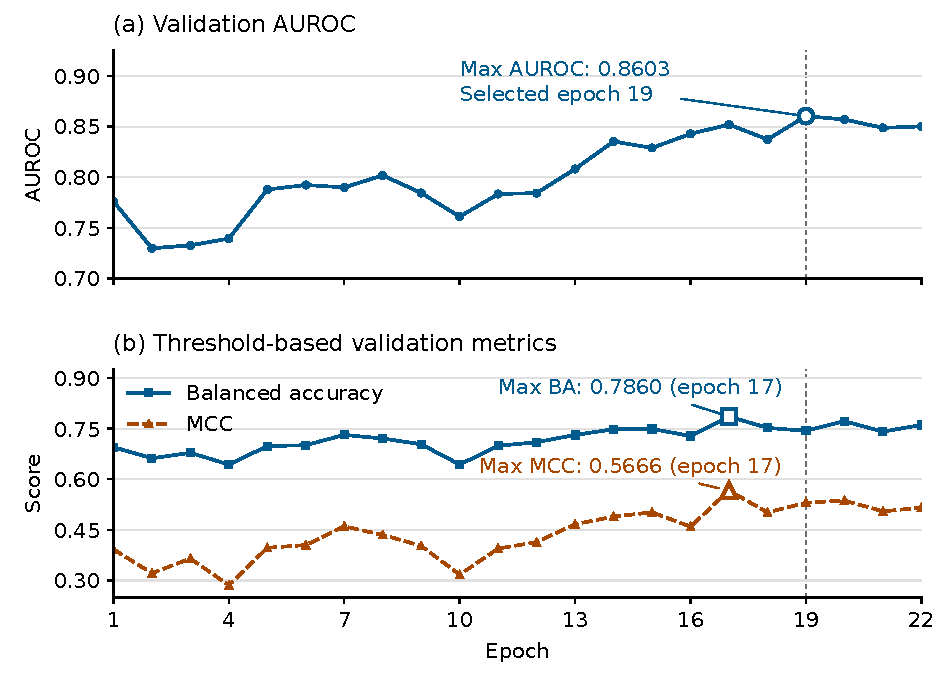
\includegraphics[width=\textwidth]{figures/raw_s42_validation.pdf}
  \caption[Diễn biến chỉ số xác thực của lần chạy raw seed 42]{%
    Diễn biến chỉ số xác thực trong 22 epoch được cung cấp của
    \texttt{raw\_s42}: (a) AUROC; (b) balanced accuracy và MCC.
    Đường thẳng đứng đánh dấu epoch 19, có AUROC cao nhất trong đoạn
    nhật ký; cực đại BA và MCC thuộc epoch 17. Các điểm được nối để
    thuận tiện quan sát, không làm trơn hoặc ngoại suy sang epoch
    chưa có dữ liệu. Hình không xác nhận việc lưu checkpoint tại các mốc này.}
  \label{fig:raw-s42-validation}
\end{figure}

Định dạng log phù hợp với notebook cũ trong Git HEAD được đối chiếu:
loss in ra là trung bình các weighted cross-entropy theo microbatch
đã chia cho \texttt{GRAD\_ACCUM}. Giá trị mặc định của hệ số này là 8,
nhưng cấu hình lịch sử chính xác chưa được xác minh độc lập. Vì vậy,
các giá trị được giữ nguyên dưới tên \textit{loss nhật ký}, không gọi
là CE thông thường, không tự nhân với 8 và không xem là validation loss.
Notebook hiện tại và \path{final_training.py} đã được cập nhật so với
triển khai cũ; objective và cách ghi loss của Trainer hiện tại khác.
Không nối trực tiếp hai đường loss, cũng không quy hồi tố các sửa đổi
hiện tại thành thuộc tính của lần chạy raw đã ghi nhận.

AUROC validation 0,8603 ở đây và AUROC \textbf{test} 0,8538 của
ResNeXt3D lịch sử (Bảng~\ref{tab:sweep-3d-leading}) chỉ là bối cảnh
không so sánh trực tiếp: khác tập đánh giá, thiết kế và quy trình.
Không tính mức cải thiện từ hai số này và không quy khác biệt cho
hợp nhất hay khử nhiễu. Sáu lần chạy fusion ConvNeXt lịch sử vẫn là
cấu hình ba nhánh 2D cộng một nhánh 3D, khác mô hình hiện tại.

\subsection{Khảo sát bộ trích xuất đặc trưng đơn nhánh 2D trên ảnh chiếu}
\label{sec:sweep-2d-results}
\subsubsection{Phạm vi và quy ước báo cáo}
Khảo sát gồm sáu cấu hình trong nhóm lần chạy ``2D feature extraction''
của dự án W\&B \texttt{glaucoma-thesis}. Theo bảng tổng hợp do tác giả
cung cấp ngày 10/09/2026, các cấu hình sử dụng ảnh chiếu en-face
Harvard-GF kích thước $224\times224$, batch size 2 và mỗi cấu hình
chỉ có một lần chạy. Số epoch hoàn thành khác nhau giữa các cấu hình.
Nguồn số liệu của mục này là bảng tổng hợp đó; việc đối chiếu trực tiếp
với lịch sử lần chạy, cấu hình xuất từ W\&B và các tệp dự đoán còn là giới hạn của khảo sát.

Các chỉ số xác thực là giá trị tại epoch cuối được ghi nhận, không
phải giá trị tốt nhất. Checkpoint dùng để tính chỉ số kiểm tra chưa
được xác định trong bảng nguồn; không mặc định đó là checkpoint cuối
hay checkpoint tốt nhất. Tên lần chạy, trạng thái tiền huấn luyện, thời gian
và toàn bộ chỉ số được trình bày tại Phụ lục~\ref{app:sweep-2d}.
Nguồn số liệu không ghi nhận precision, recall và specificity trên tập kiểm tra.
Các kết quả chỉ mô tả từng lần chạy, không có trung bình, độ lệch chuẩn hoặc khoảng tin cậy.

\begin{table}[htbp]
  \centering
  \caption{Tóm tắt khảo sát phân loại đơn nhánh 2D: một run mỗi cấu hình}
  \label{tab:sweep-2d-summary}
  \setlength{\tabcolsep}{4pt}
  \begin{tabular}{@{}lrrrrr@{}}
    \toprule
    \textbf{Cấu hình} & \textbf{Val AUROC} & \textbf{Test AUROC} & \textbf{Test F1} & \textbf{Test MCC} & \textbf{Test ECE}\\
    \midrule
    Tiny2D-AIP     & 0,7002 & 0,6605 & 0,7061 & 0,1704 & 0,0884\\
    Tiny2D-SlabAIP & 0,6307 & 0,6526 & 0,7073 & 0,2838 & 0,0550\\
    Tiny2D-SlabMIP & 0,7323 & 0,7242 & 0,7195 & 0,3210 & 0,0549\\
    ConvNeXtV2    & 0,5023 & 0,5152 & 0,7041 & 0,0000 & 0,0021\\
    DeiT3         & 0,6572 & 0,6988 & 0,6962 & 0,3040 & 0,0568\\
    MaxViT        & 0,7137 & 0,7638 & 0,7065 & 0,3765 & 0,1265\\
    \bottomrule
  \end{tabular}
\end{table}

\subsubsection{Kết quả phân loại và ảnh hưởng của biểu diễn}
Trong sáu lần chạy, MaxViT có AUROC kiểm tra cao nhất (0,7638), đồng thời
đạt accuracy 0,6889, PR-AUC 0,7925 và MCC 0,3765. Thứ hạng này đã
được tham khảo khi chọn nhánh MaxViT, nên việc lựa chọn kiến trúc
không độc lập với tập kiểm tra. Đây không phải quy tắc chọn
checkpoint của lượt tinh chỉnh cuối cùng.
Tiny2D-SlabMIP có AUROC xác thực cuối cao nhất (0,7323); trên tập
kiểm tra đạt AUROC 0,7242 và F1 cao nhất trong sáu lần chạy (0,7195).
DeiT3 đạt AUROC kiểm tra 0,6988 và MCC 0,3040.

Với cùng tên bộ trích xuất đặc trưng Tiny2D, Slab MIP đạt AUROC và MCC kiểm tra
cao hơn hai biểu diễn còn lại. AIP toàn ảnh có AUROC 0,6605, cao hơn
Slab AIP (0,6526), nhưng MCC thấp hơn (0,1704 so với 0,2838);
do đó thứ hạng hai biểu diễn này phụ thuộc chỉ số. Slab AIP có recall
xác thực 0,8125 và specificity 0,4435, thể hiện sự đánh đổi tại
ngưỡng đã dùng trong lần chạy, không đủ cơ sở để suy rộng thành hiệu quả sàng lọc.
So sánh một lần chạy cho mỗi ảnh chiếu chỉ gợi ý lựa chọn biểu diễn,
không xác lập ý nghĩa thống kê của khác biệt hoặc chứng minh tín hiệu dự đoán thuộc riêng RNFL.

\subsubsection{Hàm ý lựa chọn nhánh 2D và giới hạn}
MaxViT đã được chọn cho nhánh 2D dựa trên AUROC tập kiểm tra cao nhất trong các
lần chạy lịch sử; Tiny2D-SlabMIP được giữ làm mốc lịch sử vì F1 tập kiểm tra cao
hơn, không huấn luyện lại đối chứng. Một lần chạy không đủ xác lập ưu thế bền vững. Khảo sát MaxViT hiện ghi
Slab AIP, nên không thể suy ra hiệu năng khi đổi sang Slab MIP hoặc ba ảnh chiếu.
Đây là cơ sở lựa chọn lịch sử, không phải quy tắc chọn checkpoint cuối.
Mô hình hiện tại đã có raw validation ở Mục~\ref{sec:raw-s42-results},
nhưng chưa có kết quả Bilateral hay test; giai đoạn cuối chọn mô hình
chỉ bằng validation theo Mục~\ref{sec:final-denoise-plan}.

ConvNeXtV2 có recall xác thực bằng 0, specificity bằng 1, balanced
accuracy bằng 0,5 và MCC bằng 0; bộ chỉ số này phù hợp với dự đoán
một lớp ở ngưỡng đang dùng. Trên tập kiểm tra, balanced accuracy 0,5 và MCC 0
cũng là dấu hiệu cần kiểm tra; F1 0,7041 và ECE 0,0021 không đủ để
kết luận mô hình có khả năng phân biệt tốt. Việc đánh giá cả họ kiến trúc
đòi hỏi kiểm tra nhãn, ngưỡng, checkpoint và phân bố xác suất.
MaxViT có loss xác thực cuối 2,3924 và ECE 0,2869, cao hơn các lần chạy
còn lại; không thể xác nhận quá khớp hay chiều sai lệch độ tin cậy
chỉ từ các giá trị cuối. ECE, cách tính và thời gian được bàn luận
thêm tại Phụ lục~\ref{app:sweep-2d}. Bằng chứng hiện có không xác lập độ ổn định
qua các hạt giống ngẫu nhiên hoặc lợi ích của tổ hợp mô hình và hợp nhất đặc trưng 2D--3D.
\FloatBarrier

\subsection{Khảo sát mở rộng các bộ trích xuất đặc trưng đơn nhánh 3D}
\label{sec:sweep-3d-expanded}
\subsubsection{Phạm vi và tính tương thích của các lần chạy}
Bản tổng hợp kết quả thực nghiệm ngày 10/09/2026 ghi nhận 17 lần chạy
trong nhóm khảo sát 3D, trong đó có 16 lần chạy phân loại và một phép đo hiệu năng
khử nhiễu \texttt{denoise-gpu-2404}. Khảo sát mở rộng này được báo cáo
riêng với đợt ResNet--DenseNet--EfficientNet ở
Mục~\ref{sec:baseline-results}; không ghép hai đợt thành một bảng xếp hạng
khi chưa đối chiếu phân hoạch và quy trình đánh giá.
Theo nguồn tổng hợp, 12 lần chạy \texttt{single3d} dùng đầu vào $96^3$,
nhóm bộ trích xuất đặc trưng sau khử nhiễu dùng $200^3$ và NLM; lần chạy \texttt{3dino-112}
được trình bày riêng do thiếu cấu hình chi tiết. Mỗi cấu hình chỉ có một lần chạy.

Các khóa như \texttt{test/acc} và \texttt{test.acc} đã được quy về cùng
tên cột trong bản tổng hợp. Tuy nhiên, nguồn số liệu còn thiếu bản xuất nhật ký, định danh
checkpoint, epoch của các chỉ số trên tập xác thực và bản kê phân hoạch
để xác nhận các số liệu đến từ cùng mốc đánh giá. Việc chuẩn hóa tên
không thay thế kiểm tra ý nghĩa chỉ số. Cấu hình, bảng đầy đủ và các
trường còn thiếu được trình bày tại Mục~\ref{sec:app-3d-expanded}.

\subsubsection{Kết quả nổi bật và giới hạn xếp hạng}
Trong 12 lần chạy \texttt{single3d} được liệt kê, ResNeXt3D có các giá trị
accuracy, AUROC, PR-AUC và F1 trên tập kiểm tra cao nhất. Bảng~\ref{tab:sweep-3d-leading}
trình bày ba ứng viên có kết quả phân biệt cao trong nhóm này.
Đây là thứ hạng mô tả trên các lần chạy hiện có, không phải kết luận về
kiến trúc tối ưu hoặc kết quả lựa chọn mô hình độc lập với tập kiểm tra.

\begin{table}[htbp]
  \centering
  \caption{Kết quả trên tập kiểm tra của ba ứng viên trong khảo sát mở rộng đơn nhánh 3D}
  \label{tab:sweep-3d-leading}
  \setlength{\tabcolsep}{6pt}
  \begin{tabular}{@{}lrrrr@{}}
    \toprule
    Bộ trích xuất đặc trưng & Accuracy & AUROC & PR-AUC & F1\\ \midrule
    ResNeXt3D & \textbf{0,7711} & \textbf{0,8538} & \textbf{0,8798} & \textbf{0,7836}\\
    VNet & 0,7689 & 0,8391 & 0,8714 & 0,7763\\
    SegResNet & 0,7667 & 0,8345 & 0,8690 & 0,7737\\
    \bottomrule
  \end{tabular}
  \par\smallskip{\RaggedRight\textit{Nguồn: Bản tổng hợp kết quả thực nghiệm của tác giả.
  In đậm giá trị lớn nhất từng cột; mỗi cấu hình một lần chạy, chưa có khoảng tin cậy.}\par}
\end{table}

ResNeXt3D có balanced accuracy trên tập kiểm tra 0,7719, gần VNet (0,7718).
MCC của cả hai được ghi là 0,542 ở bảng tổng hợp; riêng VNet còn có
giá trị chi tiết 0,5417. Độ chính xác số được cung cấp của ResNeXt3D không đủ để phân định
thứ hạng MCC. ECE trên tập kiểm tra của VNet là 0,0346, thấp hơn 0,0482 của
ResNeXt3D trong các số được cung cấp; việc thiếu quy ước chia khoảng và
sai số lấy mẫu giới hạn khả năng kết luận về khác biệt hiệu chỉnh xác suất.
Accuracy trên tập xác thực của ResNeXt3D là 0,7733, chênh tập kiểm tra 0,22 điểm
phần trăm. VNet có accuracy trên tập kiểm tra cao hơn tập xác thực 2,89 điểm phần
trăm. Những chênh lệch này không tự chứng minh ổn định hay bất ổn;
cần xác nhận checkpoint; độ biến thiên qua chạy lặp vẫn chưa được đo
và không được bổ sung bằng huấn luyện mới trong phạm vi cuối.

Lần chạy \texttt{denoise-enc-32-d5} có accuracy trên tập kiểm tra cao nhất trong 16 lần chạy
phân loại được tổng hợp (0,7744), hơn ResNeXt3D 0,33 điểm phần trăm,
nhưng F1 thấp hơn (0,7772 so với 0,7836). Lần chạy này dùng $200^3$, NLM
và 20 epoch, trong khi ResNeXt3D dùng $96^3$ và 15 epoch. Các chỉ số
AUROC, PR-AUC, balanced accuracy, MCC và ECE của lần chạy khử nhiễu chưa
được cung cấp. Vì vậy, đây là đối chứng khác quy trình; không quy
chênh lệch accuracy cho riêng kiến trúc hoặc tác dụng của NLM.

\subsubsection{Dấu hiệu dự đoán một lớp và hướng kiểm chứng}
ConvNeXt3D, ViT3D và SwinUNETR cùng có accuracy trên tập kiểm tra 0,5433, F1 0,7041,
balanced accuracy 0,5 và MCC bằng 0. Tổ hợp này phù hợp với dự đoán
một lớp, như ví dụ ở Phương trình~\eqref{eq:fusion-one-class}, nhưng
cần ma trận nhầm lẫn và phân bố xác suất để xác nhận. AUROC lần lượt
là 0,5339, 0,5270 và 0,4818. Bảng chỉ số không đủ để xác định nguyên nhân;
tốc độ học, ánh xạ nhãn, ngưỡng, gradient và chính sách đóng băng
bộ trích xuất đặc trưng là các yếu tố cần kiểm chứng, không phải lỗi đã xác định.

Kết quả ConvNeXt3D đơn nhánh cũng không chứng minh đó là nguyên nhân
gây suy biến ở mô hình hợp nhất đặc trưng, vì đầu vào của mô hình này là $200^3$ và các điều kiện
khác chưa được ghép cặp.

Hai lần chạy mang tên 3DINO đã có số liệu phân loại: \texttt{single3d-3dino}
đạt AUROC trên tập kiểm tra 0,8232 và accuracy 0,7411; \texttt{3dino-112} có
accuracy 0,7522 nhưng thiếu các chỉ số còn lại. Những kết quả này
không đủ thông tin để xác định chế độ trích xuất đặc trưng hoặc
tinh chỉnh mô hình, cũng không đủ căn cứ khái quát rằng CNN
luôn vượt Transformer hay mô hình sâu hơn không có lợi ích.

ResNeXt3D đã được chọn cho nhánh 3D; VNet, SegResNet và
\texttt{denoise-enc-32-d5} chỉ được giữ làm mốc lịch sử khác quy trình,
không huấn luyện lại làm đối chứng. Raw validation của mô hình hiện tại
đã có, còn kết quả Bilateral và test đang chờ. Không thực hiện thêm
3--5 seed hay khảo sát cấu hình: phạm vi cập nhật trọng số còn lại chỉ
là một lần fine-tune 10 epoch tại Mục~\ref{sec:final-denoise-plan}.
Vì thứ hạng test lịch sử đã được tham khảo để đề xuất ứng viên, test
trên cùng nguồn không được coi là xác nhận độc lập hoàn toàn đối với
quá trình lựa chọn thiết kế; giai đoạn cuối không tiếp tục dùng test để chọn mô hình.
\FloatBarrier

\subsubsection{Khảo sát bổ sung mô hình 3D sau NLM}
Bảng~\ref{tab:denoise-enc32} trong
Mục~\ref{sec:sweep-3d-denoise-enc32} tổng hợp kết quả xác thực của
\texttt{denoise-enc-32} qua 20 epoch. Accuracy cao nhất khoảng
0,780 tại epoch 17 và F1 cao nhất khoảng 0,827 tại epoch 14;
đây là các số xấp xỉ đọc từ biểu đồ của lần khảo sát trước. Việc thiếu
mã định danh lần chạy và checkpoint không cho phép xác nhận mối liên hệ giữa lịch sử này với accuracy
trên tập kiểm tra 0,7533 và F1 0,7668 của lần chạy cùng tên trong bản tổng hợp mới.
Các kết quả được giữ để đối chiếu mô hình 3D, không được xem là
bằng chứng riêng về hiệu quả khử nhiễu NLM.

\subsection{Khảo sát hợp nhất đặc trưng 2D--3D}
\label{sec:group-a-results}
\label{sec:fusion-sweep-results}
\subsubsection{Phạm vi khảo sát và checkpoint}
Theo bảng tổng hợp kết quả thực nghiệm ngày 10/09/2026, khảo sát gồm
sáu phương pháp: Concat, Add, Attention, CrossGate, Mamba và FiLM,
mỗi phương pháp một lần chạy. Mô hình nhận ba ảnh 2D $224\times224$
qua ConvNeXtV2-Tiny và một khối ảnh 3D $200^3$ qua ConvNeXt3D;
batch size 2, số epoch tối đa 10. Đây là cấu hình bổ sung, khác
cấu hình MaxViT--ResNeXt3D ở Mục~\ref{sec:group-a}.
Thông tin chi tiết và các trường cần đối chiếu được lưu tại
Phụ lục~\ref{app:fusion-sweep}.

Bảng nguồn xác định epoch đạt AUC xác thực cao nhất cho từng lần chạy.
Trong phần này, AUC được trình bày dưới tên AUROC để thống nhất thuật
ngữ; cách tính cần được xác nhận từ nhật ký và mã nguồn. Chỉ số PR-AUC
xác thực được lấy cùng epoch đó, còn loss nhỏ nhất có thể thuộc epoch
khác. Kết quả trên tập kiểm tra được báo cáo riêng vì thông tin cung cấp không ghi
đường dẫn hoặc mã checkpoint đã nạp khi kiểm tra. Do vậy, không thể mặc
định kết quả kiểm tra được tính tại checkpoint có AUROC xác thực cao nhất.

\begin{table}[htbp]
  \centering
  \caption{Tóm tắt sáu lần chạy hợp nhất đặc trưng 2D--3D}
  \label{tab:fusion-summary}
  \setlength{\tabcolsep}{6pt}
  \begin{tabular}{@{}lrrr@{}}
    \toprule
    Phương pháp & Epoch chọn & Best Val AUROC & Test AUROC\\
    \midrule
    Concat & 2 & 0,5302 & 0,5031\\
    Add & 6 & 0,5389 & 0,4914\\
    Attention & 4 & 0,5664 & 0,5205\\
    CrossGate & 1 & 0,5690 & \textbf{0,5685}\\
    Mamba & 6 & \textbf{0,6056} & 0,4715\\
    FiLM & 4 & 0,5718 & 0,5028\\
    \bottomrule
  \end{tabular}
\end{table}

\subsubsection{Kết quả và dấu hiệu dự đoán một lớp}
Mamba có AUROC xác thực cao nhất trong sáu lần chạy (0,6056 tại epoch 6),
nhưng AUROC trên tập kiểm tra chỉ 0,4715. CrossGate có AUROC trên tập kiểm tra cao nhất
(0,5685) và PR-AUC trên tập kiểm tra 0,5981. Thứ hạng này chỉ mô tả các lần chạy,
không dùng để chọn phương pháp theo tập kiểm tra và không chứng minh khác
biệt có ý nghĩa thống kê. Attention có mức giảm AUROC từ đỉnh đến
cuối nhỏ nhất trong bảng nguồn, nhưng hai mốc này chưa đủ mô tả
dao động toàn bộ đường học hoặc độ ổn định qua các hạt giống ngẫu nhiên.

Tất cả phương pháp cùng đạt accuracy trên tập kiểm tra 0,5433, F1 0,7041,
balanced accuracy 0,5000 và MCC 0,0000. Tổ hợp này phù hợp với
trường hợp dự đoán toàn bộ mẫu về lớp dương; phần ghi chú nguồn
cũng báo cáo recall trên tập xác thực bằng 1 và specificity bằng 0,
nhưng chưa chỉ rõ epoch. Phụ lục~\ref{app:fusion-sweep} minh họa
vì sao F1 khá cao vẫn có thể xuất hiện khi dự đoán một lớp.
Cần kiểm tra ma trận nhầm lẫn và xác suất từng mẫu để xác nhận.

Các kết quả lịch sử này chưa xác lập lợi ích của hợp nhất đặc trưng.
Việc rà soát nhãn, checkpoint, ngưỡng và đầu ra có thể dùng mã nguồn
và dự đoán đã lưu, nhưng không kèm huấn luyện lại đối chứng đơn nhánh
hay hợp nhất. Raw validation mới được báo cáo riêng tại
Mục~\ref{sec:raw-s42-results}, chưa chứng minh lợi ích tăng thêm của fusion.
Dấu hiệu suy biến trong lần chạy ConvNeXtV2 đơn nhánh ở Mục~\ref{sec:sweep-2d-results}
gợi ý một hướng kiểm tra, nhưng không chứng minh bộ trích xuất đặc trưng 2D là nguyên nhân
của hiện tượng trong các lần chạy hợp nhất. Kết quả âm tính của khảo sát
này cũng không đủ để bác bỏ toàn bộ hướng hợp nhất đặc trưng 2D--3D.
\FloatBarrier

\subsection{Khảo sát nền phục vụ xây dựng mô hình đa nhánh}
\label{sec:baseline-results}
Các thí nghiệm sau được thực hiện trước để khảo sát khả năng học
từ khối ảnh 3D và chi phí kiến trúc. Chúng hỗ trợ lựa chọn đường
cơ sở, nhưng không phải đối chứng ghép cặp đã hoàn tất của mô hình
đa nhánh. Việc thiếu cùng phân hoạch và điều kiện huấn luyện giới hạn
so sánh trực tiếp; không bổ sung các lần chạy này trong phạm vi cuối.
\subsubsection{Khảo sát đầu vào 3D ở độ phân giải đầy đủ}

% Không tạo một tiểu mục đánh số đơn lẻ (Mẫu 10, tr. 8).
\mucthu{Thử nghiệm trên 400 khối ảnh kích thước $200^3$}
Trong lần thử đầu tiên, ResNet152 và DenseNet121 được huấn luyện trên 400 khối ảnh ở độ phân giải $200\times200\times200$. Các đường mất mát và độ chính xác
dao động mạnh, không cho thấy xu hướng giảm mất mát hoặc tăng độ chính
xác một cách ổn định. Vì vậy, lần thử này không cung cấp bằng chứng rằng hai mô
hình đã học được một biểu diễn có khả năng khái quát từ đầu vào 3D độ phân giải
đầy đủ.

Kết quả này góp phần định hướng thiết kế nghiên cứu. Một khối ảnh $200^3$
có số voxel lớn hơn khoảng chín lần khối ảnh $96^3$, trong khi các mạng 3D sâu
còn phải lưu các bản đồ kích hoạt trung gian trong quá trình lan truyền ngược.
Do đó, việc giữ độ phân giải gốc làm tăng đáng kể yêu cầu bộ nhớ và thời gian
tính toán, hạn chế kích thước batch và có thể làm gradient nhiễu hơn. Trên cơ sở
đó, nghiên cứu chuyển sang độ phân giải $96^3$ để xây dựng một đường cơ sở khả
thi về tính toán.

\subsubsection{Khảo sát các kiến trúc tại độ phân giải \texorpdfstring{$96^3$}{96x96x96}}

\mucthu{Độ chính xác xác thực và kiểm tra}
Kết quả đầy đủ của ba họ mô hình được trình bày tại
Bảng~\ref{tab:sweep-accuracy}, Mục~\ref{sec:app-3d-baseline}.
Xét riêng độ chính xác xác thực, DenseNet169 đạt giá trị cao nhất
là 0,8100. Tuy nhiên, độ
chính xác kiểm tra của mô hình này chỉ đạt 0,7467, thấp hơn 0,0633 so với kết quả
xác thực. ResNet18 không đứng đầu trên tập xác thực nhưng đạt độ chính xác kiểm
tra cao nhất, 0,7722. Sự thay đổi thứ hạng giữa hai tập cho thấy lựa chọn mô hình
chưa ổn định và không nên chỉ dựa trên một lần chia dữ liệu.





Trong nhóm năm mô hình có độ chính xác xác thực cao nhất, DenseNet chiếm ba vị
trí. Dù vậy, DenseNet169 không phải mô hình tốt nhất trên tập kiểm tra. Kết quả
này cho thấy con số 0,8100 nên được xem là kết quả lựa chọn mô hình trên tập xác
thực, không phải bằng chứng độc lập về độ chính xác tổng quát. Với EfficientNet,
việc tăng kích thước từ B0 đến B7 không tạo ra cải thiện đơn điệu; EfficientNet-B7
chỉ đạt 0,5433 trên tập kiểm tra. Như vậy, tăng độ sâu hoặc số tham số không tự
động khắc phục hạn chế của biểu diễn đầu vào.

% ===== TẠM ẨN: giữ nguyên nội dung, bỏ tiền tố comment để khôi phục =====
% \subsubsection{Chi phí tính toán}
% Số liệu chi tiết về tài nguyên được trình bày tại
% Bảng~\ref{tab:sweep-resource}, Mục~\ref{sec:app-3d-baseline}.
% Trong khảo sát này, DenseNet169 sử dụng 18,5 triệu
% tham số, 4,1~GB VRAM và 14,1 giây mỗi epoch. Trong khi đó, ResNet152 cần
% 31,2~GB VRAM và 84,9 giây mỗi epoch nhưng có độ chính xác xác thực thấp hơn.
% ResNet200 không thể chạy do hết bộ nhớ.
%
% Từ khảo sát nền, DenseNet169 là cấu hình tham chiếu đáng cân nhắc
% theo độ chính xác xác thực và chi phí đã ghi nhận, nhưng không được
% đồng nhất với backbone của mô hình đa nhánh. Nhánh 3D trong thiết kế
% đề xuất dùng mạng residual 3D tùy chỉnh \texttt{Enc3D}, với lý do và
% cấu trúc nêu tại Mục~\ref{sec:branch-backbones}. Hai bảng ở
% Mục~\ref{sec:app-3d-baseline} chưa chứng minh ưu thế của lựa chọn này;
% kết luận cuối cùng cần dựa trên thực nghiệm cùng điều kiện đầu vào
% và phân hoạch dữ liệu.
%
%
%
% Các số liệu trên ủng hộ việc dùng $96^3$ làm đường cơ sở thực dụng trong giai
% đoạn phát triển. Việc quay lại độ phân giải $128^3$ hoặc $200^3$ chỉ nên được
% thực hiện khi có đủ bộ nhớ, có chiến lược huấn luyện như crop theo vùng quan tâm,
% gradient accumulation hoặc mixed precision, và có đối chứng cho thấy phần thông
% tin không gian bổ sung thực sự cải thiện kết quả.
%
% ===== KẾT THÚC KHỐI TẠM ẨN =====

\subsection{Tóm tắt khảo sát tiền xử lý bổ trợ}
Khảo sát sáu bộ lọc trên 14 thể tích và khảo sát bổ sung bảy bộ lọc
trên khối \texttt{data\_2404} được trình bày tại
Phụ lục~\ref{app:denoise-support}. Đánh giá đa tiêu chí ưu tiên
Bilateral cho vòng kiểm chứng tiếp theo, nhưng chưa chứng minh
lợi ích phân loại; thời gian giữa các lần chạy không thuộc phép đo hiệu năng
thống nhất. Kết quả mô hình 3D sau NLM được tổng hợp tại
Mục~\ref{sec:sweep-3d-denoise-enc32}, tách biệt với đánh giá chất
lượng ảnh của bộ lọc.

\section{Đánh giá đóng góp thành phần và giới hạn đối chứng}
\label{sec:ablation}
\subsection{Phạm vi bằng chứng hiện có}
Các lần chạy đơn nhánh cung cấp kết quả khảo sát bộ trích xuất đặc trưng,
còn sáu lần chạy hợp nhất khảo sát các cơ chế trên ConvNeXtV2--ConvNeXt3D.
Những kết quả này không tạo thành đối chứng đóng góp thành phần đầy đủ
của quy trình Bilateral--MaxViT--ResNeXt3D. Bằng chứng còn thiếu gồm
cặp ảnh gốc--Bilateral dùng cùng bộ trích xuất đặc trưng và cặp mô hình
đầy đủ--loại bỏ nhánh được huấn luyện theo cùng quy tắc.

Ba cấu hình Tiny2D theo ảnh chiếu cung cấp quan sát về vai trò biểu
diễn, nhưng không thay thế đối chứng loại bỏ ảnh chiếu trong mô hình MaxViT đa
nhánh. Kết quả khử nhiễu trên một khối ảnh cũng không đo đóng góp của
bộ lọc đối với phân loại. Raw validation đã có nhưng denoise và test
chưa có; mục này xác định giới hạn so sánh trước--sau,
không báo cáo mức cải thiện hoặc kiểm định khi chưa có dự đoán thực tế.

\subsection{Giới hạn của so sánh trước--sau và phép bỏ nhánh}
Kế hoạch ở Mục~\ref{sec:final-denoise-plan} không phải đối chứng
denoising có ngân sách huấn luyện bằng nhau. Một seed, 10 epoch học
thêm và thay đổi triển khai/cache không cho phép cô lập tác động của
bộ lọc. Không suy ra ưu thế kiến trúc từ việc so sánh các bảng khác
phân hoạch, đầu vào hoặc tiêu chí chọn checkpoint.

Branch-drop trên mô hình đóng băng có thể mô tả độ nhạy của đầu ra
khi thiếu một nhánh, nhưng không tương đương huấn luyện lại mô hình
không có nhánh đó. Các tương tác giữa nhánh, thay đổi phân phối đầu
vào và cách che đặc trưng giới hạn diễn giải nhân quả. Không thực
hiện training ablation, raw control hoặc seed bổ sung trong phạm vi cuối.
\FloatBarrier

\section{Phân tích định tính và XAI}
\label{sec:qualitative-xai}
\subsection{Kế hoạch giải thích với trọng số cố định}
Phần này là kế hoạch sau lần fine-tune cuối, không phải kết quả đã
quan sát. Sau khi chọn checkpoint bằng validation và đóng băng mô
hình, Grad-CAM, Integrated Gradients (IG), occlusion, bản đồ attention
và branch-drop có thể được dùng để khảo sát vùng ảnh hoặc nhánh liên
quan đến đầu ra. Gradient phục vụ giải thích không đi kèm optimizer
step, không cập nhật trọng số hoặc trạng thái thống kê của mô hình.

Các hình dự kiến cần ghi định danh mẫu, nhãn, điểm số, checkpoint,
nhánh và cách dựng bản đồ; với IG ghi ảnh nền tham chiếu, với occlusion
ghi vùng che và cách thay giá trị. Đối chiếu mẫu dự đoán đúng và sai
theo quy tắc lựa chọn công bố trước, không chỉ chọn hình phù hợp với
giả thuyết. Attention hoặc vùng sáng trên bản đồ không tự chứng minh
mô hình dựa vào RNFL hay một cơ chế bệnh học đã được xác nhận.

% ------------------------- PHẦN CUỐI -------------------------
\subsection{Phân tích lỗi và giới hạn diễn giải}
Ma trận nhầm lẫn, phân bố điểm số và các trường hợp dương tính giả,
âm tính giả là cơ sở phân tích lỗi. Việc quy nguyên nhân cho kiến trúc
đòi hỏi kiểm tra hướng ảnh, giả ảnh và dải tạo ảnh chiếu. Phạm vi kết quả
hiện có không bao gồm trực quan hóa đặc trưng hoặc bản đồ giải thích;
những phân tích này thuộc hướng kiểm chứng tiếp theo, không phải bằng chứng
thực nghiệm đã hoàn thành.

\section{Phân tích chi phí và khả năng tái lập}
\label{sec:cost-reproducibility}
\subsection{Bằng chứng chi phí và giới hạn đối chiếu}
Số tham số, VRAM và thời gian của khảo sát nền được giữ tại
Bảng~\ref{tab:sweep-resource}; thời gian các lần chạy 2D nằm tại
Phụ lục~\ref{app:sweep-2d}. Đây là số đo lịch sử, không phải chi phí
của mô hình hiện tại. Các phép đo bộ lọc trên khối \texttt{data\_2404}
dùng Windows và CPU 12 luồng; khoảng 3,6 giờ tạo cache NLM thuộc
quy trình khác, không so trực tiếp với thời gian đọc cache hoặc GPU.
Chi tiết phạm vi đo nằm tại Mục~\ref{sec:denoise-comparison-method}.

Nhật ký raw 22 epoch chưa cung cấp thời gian mỗi epoch, tổng thời
gian, VRAM cực đại hoặc độ trễ suy luận đã xác minh. Không suy ra
chi phí của mô hình hai nhánh 2D cộng một nhánh 3D từ số đo fusion
ConvNeXt ba nhánh 2D lịch sử, cũng không ngoại suy thời gian hoàn
thành 30 epoch. Thiếu số đo được ghi là chưa có, không mở thêm lần
huấn luyện để bổ sung bảng chi phí. Số đo phát sinh trong lần fine-tune
duy nhất hoặc đánh giá mô hình cố định, nếu được lưu, phải tách thời
gian tiền xử lý, I/O và suy luận. Định nghĩa số tham số, đơn vị bộ nhớ
và thời gian được giữ tại Mục~\ref{sec:evaluation-metrics}.

\subsection{Hồ sơ tái lập và phân biệt phiên bản}
Hồ sơ cần gắn checkpoint với epoch, seed, phiên bản mã và thư viện,
phân hoạch mẫu, cấu hình tiền xử lý, cache và phần cứng thực dùng.
Nhật ký CSV raw và checkpoint được bảo toàn; bản xuất W\&B, dự đoán
cấp mẫu và artifact trên Drive của giai đoạn cuối phải mang định danh
riêng, không ghi đè bằng chứng legacy. Thiếu metadata lịch sử không
được điền bằng giá trị mặc định của notebook hiện tại.

Sự khác biệt objective và cách ghi loss giữa notebook legacy với
notebook hiện tại/\path{final_training.py} ngăn việc nối trực tiếp
đường loss. Đánh giá lại trọng số khởi tạo bằng quy trình hiện tại
được lưu như phép đánh giá mới, không sửa lại số liệu lịch sử. Việc
xác minh này phục vụ một lần warm-start denoise và đánh giá đóng băng,
không phải cam kết tái huấn luyện các khảo sát để tái lập kết quả.

\section{Thảo luận}
\label{sec:auxiliary-analysis}

\subsection{Đánh giá giả thuyết về mô hình đơn nhánh 3D}
Khảo sát nền trước đây ghi nhận đường học dao động ở $200^3$ và thay đổi
thứ hạng giữa tập xác thực và tập kiểm tra ở $96^3$. Khảo sát mở rộng bổ sung
ResNeXt3D với AUROC trên tập kiểm tra 0,8538 và F1 0,7836, cho thấy không nên
khái quát hạn chế của những lần chạy ban đầu cho mọi bộ trích xuất đặc trưng 3D.
Tuy nhiên, việc thiếu chạy lặp, khoảng tin cậy và đối chứng cùng điều kiện
giới hạn khả năng xác nhận hiệu quả bền vững hoặc lợi ích tăng thêm của hợp nhất đặc trưng.
Các đường học trước đây không mô tả độ ổn định của những lần chạy mới.

Có ít nhất ba cách giải thích chưa thể loại trừ. Thứ nhất, số mẫu của khảo sát có
thể quá nhỏ so với độ phức tạp của mạng 3D. Thứ hai, phép giảm kích thước xuống
$96^3$ có thể làm mất các cấu trúc nhỏ liên quan đến bệnh. Thứ ba, nhãn chẩn đoán
có thể liên quan đến những dấu hiệu được mô hình khai thác thuận lợi hơn trên
ảnh chiếu 2D từ cùng khối ảnh. Do đó, kết quả hiện tại không đủ để xem
mô hình 3D đơn là một lời giải đã được kiểm chứng, cũng không chứng minh
rằng dữ liệu 3D không chứa thông tin dự đoán.

\subsection{Giới hạn suy luận về vai trò của ảnh chiếu}
Kết quả kém của một cấu hình không chứng minh khối OCT thiếu tín hiệu
phân loại. Các ảnh chiếu là biến đổi xác định của cùng khối ảnh, không
phải phép đo độc lập mới. Nếu mô hình hợp nhất cải thiện hiệu năng,
cần kiểm tra đóng góp của biểu diễn, số tham số và quy trình tối ưu
bằng các đối chứng cùng điều kiện, thay vì quy toàn bộ cải thiện cho cơ chế hợp nhất đặc trưng.

\subsection{Hàm ý của kết quả nghiên cứu}
Các khảo sát nền và sáu lần chạy hợp nhất đặc trưng chưa chứng minh ưu thế của mô
hình đa nhánh. Khảo sát ConvNeXtV2--ConvNeXt3D cần được kiểm tra
hiện tượng dự đoán một lớp trước khi xếp hạng các cơ chế hợp nhất.
Mô hình hiện tại đã có tín hiệu học tích cực trên raw validation,
nhưng Bilateral và lợi ích tăng thêm của từng nhánh chưa được chứng minh.
Không ghép các khảo sát đơn nhánh và hợp nhất khác điều kiện thành một
phép so sánh trực tiếp. Các đối chứng huấn luyện còn thiếu được ghi
nhận là hạn chế, không bổ sung vào phạm vi cuối.

So sánh raw--denoise còn lại tuân theo Mục~\ref{sec:final-denoise-plan}:
một lần fine-tune 10 epoch rồi đóng băng. Dù chỉ số tăng hay giảm,
phải báo cáo trung thực và không quy riêng cho bộ lọc; không mở thêm
vòng huấn luyện hoặc điều chỉnh Bilateral theo test. Grad-CAM và
bản đồ sai khác chỉ hỗ trợ diễn giải, không tự xác nhận RNFL được bảo toàn.

\subsection{Đối chiếu với câu hỏi nghiên cứu}
Đối với CH1 ở Mục~\ref{sec:research-questions}, raw seed 42 cung cấp
mốc validation quan sát, nhưng chưa có kết quả sau fine-tune denoise
để mô tả thay đổi trước--sau. Kế hoạch 10 epoch không nhằm cô lập
tác động nhân quả của Bilateral khỏi tối ưu hóa bổ sung và thay đổi
triển khai/cache; số đo chất lượng ảnh không trả lời thay câu hỏi này.

Đối với CH2, các khảo sát cung cấp khả năng phân biệt, độ cân bằng
lớp và chi phí trong từng điều kiện, làm căn cứ lựa chọn MaxViT và
ResNeXt3D. Chúng không xác lập thứ hạng bền vững qua seed hoặc so sánh
kiến trúc có kiểm soát. AUROC validation 0,8603 ở epoch 19 của raw
không được dùng để tuyên bố vượt AUROC test 0,8538 của ResNeXt3D lịch sử.

Đối với CH3, phân tích dự đoán, hậu xử lý và XAI trên mô hình hai
nhánh 2D cộng một nhánh 3D đóng băng vẫn là kế hoạch tại
Mục~\ref{sec:qualitative-xai}, chưa có kết quả để kết luận về vùng
ảnh được sử dụng hay các trường hợp sai. Dấu hiệu dự đoán một lớp
của fusion ConvNeXt lịch sử không được gán cho mô hình hiện tại.
Branch-drop khi suy luận không thay thế training ablation; giới hạn
diễn giải đóng góp thành phần được nêu tại Mục~\ref{sec:ablation}.

\section{Tóm tắt chương}
Chương này tách thiết lập vận hành khỏi các định nghĩa bổ trợ tại
Phụ lục~\ref{app:supporting-methods}, đồng thời phân biệt kết quả
raw validation với các khảo sát lịch sử và phần việc chưa thực hiện.
Raw seed 42 có 22 epoch quan sát, AUROC validation cao nhất 0,8603
ở epoch 19; BA/MCC cao nhất thuộc epoch 17. Chưa có test hoặc kết
quả denoise của mô hình hiện tại, nên chưa xác nhận lợi ích Bilateral
hay đóng góp độc lập của từng nhánh. Phạm vi còn lại là một lần
warm-start denoise 10 epoch từ trọng số đã xác minh, sau đó chỉ đánh
giá, hậu xử lý và XAI với mô hình đóng băng.

\chapter{Kết luận và hướng phát triển}
\label{chap:conclusion}
\section{Tóm tắt kết quả}
Luận văn nghiên cứu bài toán phân loại glaucoma
từ ảnh OCT B-scan và các ảnh chiếu tương ứng.
Thiết kế hiện tại kết hợp một nhánh 3D nhận khối $200^3$ và hai nhánh 2D thông qua
khối hợp nhất đặc trưng. Đến thời điểm tổng hợp, đã có kết quả
khảo sát đơn nhánh 2D, nền 3D và sáu lần chạy hợp nhất đặc trưng trên cấu hình
ConvNeXtV2--ConvNeXt3D. Tuy nhiên, các lần chạy hợp nhất có dấu hiệu
dự đoán một lớp và thiếu đối chứng tương ứng đầy đủ để xác nhận
lợi ích hợp nhất. Khảo sát ConvNeXt lịch sử dùng ba nhánh 2D, không
đồng nhất với mô hình hiện tại. Riêng raw seed 42 đã quan sát 22 epoch
trong ngân sách danh nghĩa 30, đạt AUROC validation tốt nhất 0,8603
tại epoch 19 với BA 0,7437, MCC 0,5307 và loss nhật ký 0,0656.
BA/MCC tốt nhất 0,7860/0,5666 thuộc epoch 17, không ghép với đỉnh
AUROC thành một checkpoint. Chưa có kết quả denoise hay test của
mô hình này và chưa có căn cứ xác nhận hoàn thành 30 epoch hoặc early stopping.

Khảo sát ban đầu cho thấy huấn luyện ResNet152 và DenseNet121 trên 400 khối ảnh
$200^3$ không tạo ra đường học ổn định. Khi giảm độ phân giải xuống $96^3$,
DenseNet169 đạt độ chính xác xác thực cao nhất là 0,8100, còn ResNet18 đạt độ
chính xác kiểm tra cao nhất là 0,7722. Tuy nhiên, sự thay đổi thứ hạng giữa tập
xác thực và tập kiểm tra, cùng với các đường học dao động, cho thấy chưa đủ bằng
chứng để kết luận về độ ổn định của các cấu hình trong đợt khảo sát này.

Đợt khảo sát 3D mở rộng bổ sung 16 lần chạy phân loại. ResNeXt3D có AUROC
trên tập kiểm tra 0,8538 và F1 0,7836, cao nhất trong các giá trị được cung cấp;
\texttt{denoise-enc-32-d5} có accuracy cao nhất 0,7744 nhưng dùng
quy trình khác. ResNeXt3D là nhánh 3D đã chọn, VNet và
SegResNet là mốc lịch sử, không phải các lần huấn luyện tiếp theo.
Việc từng tham khảo test để chọn thiết kế giới hạn tính độc lập của
đánh giá trên cùng nguồn. AUROC test 0,8538 không so trực tiếp với
AUROC validation 0,8603 của raw seed 42. Các kết quả này không thay thế đối chứng hợp nhất đặc trưng
dùng cùng bộ trích xuất đặc trưng và điều kiện huấn luyện.

Khảo sát sáu cấu hình 2D cung cấp thêm kết quả phân loại từ ảnh chiếu.
MaxViT đạt AUROC kiểm tra cao nhất 0,7638; Tiny2D-SlabMIP đạt AUROC
xác thực cuối cao nhất 0,7323 và F1 kiểm tra cao nhất 0,7195.
Trong ba lần chạy Tiny2D, Slab MIP có AUROC và MCC kiểm tra cao nhất,
gợi ý vai trò của biểu diễn trong khảo sát lịch sử. Tuy nhiên,
mỗi cấu hình chỉ có một lần chạy, checkpoint dùng để đánh giá trên tập kiểm tra chưa được xác nhận
và điều kiện không được ghép cặp với khảo sát hợp nhất đặc trưng; các thứ hạng này không xác lập
bộ trích xuất đặc trưng tối ưu hoặc độ ổn định của mô hình đa nhánh.

Trong sáu lần chạy hợp nhất đặc trưng, Mamba đạt AUROC xác thực tốt nhất 0,6056,
trong khi CrossGate đạt AUROC trên tập kiểm tra cao nhất 0,5685. Tất cả lần chạy có
accuracy trên tập kiểm tra 0,5433, F1 0,7041, balanced accuracy 0,5 và MCC bằng 0.
Tổ hợp chỉ số phù hợp với dự đoán một lớp, nên không diễn giải F1
như bằng chứng phân loại tốt. Việc thiếu xác nhận checkpoint và
đối chứng cùng điều kiện là hạn chế của khảo sát này, không phải
yêu cầu thực hiện lại huấn luyện trong giai đoạn cuối.

Các kết quả khử nhiễu được giữ tại Phụ lục~\ref{app:denoise-support}.
Việc thiếu đối chứng phân loại ảnh gốc--khử nhiễu ghép cặp không cho phép
xác nhận bộ lọc tốt nhất cho bài toán. Bilateral được chọn để kiểm
chứng tiếp trên cơ sở đánh đổi chất lượng ảnh, không phải vì đã có
kết quả phân loại vượt trội.

\section{Đóng góp}
Luận văn hệ thống hóa các khảo sát thực nghiệm làm căn cứ chọn thành
phần, đề xuất giao diện hợp nhất đặc trưng 2D--3D và xác định quy trình
đối chứng cho bài toán phân loại OCT. Phân tích đồng thời AUROC, F1,
balanced accuracy và MCC làm rõ giới hạn của việc diễn giải accuracy
hoặc F1 riêng lẻ khi mô hình có dấu hiệu dự đoán một lớp.

Đóng góp hiện có là thiết kế, phân tích bằng chứng khảo sát và bổ sung
lịch sử raw validation 22 epoch của mô hình hiện tại. Lợi ích
của Bilateral và của tổ hợp MaxViT--ResNeXt3D chưa được xác nhận bằng
đối chứng đóng góp thành phần. Vì vậy, việc kết hợp các thành phần đã công bố
không được diễn giải là một kiến trúc mới đã chứng minh ưu thế.

\section{Hạn chế}
Hạn chế của khảo sát hợp nhất ConvNeXt lịch sử là dấu hiệu dự đoán một lớp,
mỗi phương pháp chỉ có một lần chạy và checkpoint dùng để đánh giá trên tập kiểm tra
chưa được xác nhận. Bằng chứng còn thiếu đối chứng đơn nhánh--đa nhánh đầy đủ
trong cùng điều kiện. Khảo sát nền 3D trước đây thiếu các chỉ số ngoài accuracy
và có giá trị epoch không nhất quán; đợt 3D mở rộng đã bổ sung nhiều chỉ số
nhưng thiếu siêu dữ liệu, thông tin checkpoint và kết quả chạy lặp.
Khảo sát 2D đã bổ sung AUROC, PR-AUC, F1, MCC và ECE, nhưng chỉ có một
lần chạy mỗi cấu hình, thiếu precision, recall, specificity trên tập kiểm tra
và thông tin checkpoint.
Raw seed 42 chỉ có một seed và 22 epoch quan sát, chưa xác minh độc
lập đầy đủ cấu hình legacy và nguồn tệp trọng số epoch tốt nhất,
chưa có test hay kết quả denoise. Loss nhật ký không được coi là CE
thông thường hoặc nối trực tiếp với loss của Trainer đã sửa. So sánh
trước--sau dự kiến còn lẫn tác động của 10 epoch học thêm, triển khai
và cache, nên không thể cô lập lợi ích của khử nhiễu.

\section{Hướng phát triển ngoài phạm vi luận văn}
Nghiên cứu tiếp nối có thể xem xét dữ liệu độc lập từ cơ sở hoặc
thiết bị khác, đối chứng có ngân sách tối ưu bằng nhau, nhiều seed
và đánh giá lâm sàng phù hợp điều kiện sử dụng dữ liệu. Đây là các
hướng ngoài phạm vi, không phải nhiệm vụ huấn luyện bắt buộc để
hoàn tất luận văn này và không được coi là bằng chứng đã có.

Phạm vi hoàn thiện hiện tại vẫn chỉ là một lần warm-start denoise
10 epoch tại Mục~\ref{sec:final-denoise-plan}, sau đó chỉ đánh giá,
hậu xử lý và XAI với mô hình đóng băng; không thêm raw control,
seed, training ablation hay mô hình mới. Raw validation cho tín
hiệu học tích cực, nhưng chưa có bằng chứng về lợi ích denoising
cho đến khi có kết quả thực tế. Ngay cả so sánh trước--sau dự kiến
cũng không đủ để quy tác động nhân quả riêng cho bộ lọc.

\clearpage
\phantomsection
\addcontentsline{toc}{chapter}{DANH MỤC TÀI LIỆU THAM KHẢO}
\begin{thebibliography}{99}
\RaggedRight
\item[]\textbf{Tiếng Anh}

\bibitem{aum2015}
Aum, J., Kim, J.-h. and Jeong, J. (2015), ``Effective speckle noise suppression
in optical coherence tomography images using nonlocal means denoising filter
with double Gaussian anisotropic kernels'', \textit{Applied Optics}, 54(13),
pp.~D43--D50.

\bibitem{bm3dSoftware}
BM3D developers, \textit{bm3d: Python wrapper for BM3D denoising},
\url{https://pypi.org/project/bm3d/}, truy cập ngày 08/09/2026.

\bibitem{buades2005}
Buades, A., Coll, B. and Morel, J.-M. (2005), ``A non-local algorithm for image
denoising'', \textit{Proceedings of the IEEE Computer Society Conference on
Computer Vision and Pattern Recognition}, Vol.~2, pp.~60--65.

\bibitem{chambolle2004tv}
Chambolle, A. (2004), ``An algorithm for total variation minimization and
applications'', \textit{Journal of Mathematical Imaging and Vision},
20, pp.~89--97.

\bibitem{chang2000wavelet}
Chang, S. G., Yu, B. and Vetterli, M. (2000), ``Adaptive wavelet thresholding
for image denoising and compression'', \textit{IEEE Transactions on Image
Processing}, 9(9), pp.~1532--1546.

\bibitem{dabov2007bm3d}
Dabov, K., Foi, A., Katkovnik, V. and Egiazarian, K. (2007), ``Image denoising
by sparse 3-D transform-domain collaborative filtering'', \textit{IEEE
Transactions on Image Processing}, 16(8), pp.~2080--2095.

\bibitem{gholami2018octid}
Gholami, P., Roy, P., Parthasarathy, M. K. and Lakshminarayanan, V.
(2018), ``OCTID: Optical Coherence Tomography Image Database'',
\textit{arXiv preprint}, arXiv:1812.07056,
phiên bản cập nhật năm 2019.

\bibitem{guedes2003oct}
Guedes, V., Schuman, J. S., Hertzmark, E., Wollstein, G., Correnti, A.,
Mancini, R., Lederer, D., Voskanian, S., Velazquez, L., Pakter, H. M.,
Pedut-Kloizman, T., Fujimoto, J. G. and Mattox, C. (2003),
``Optical coherence tomography measurement of macular and nerve fiber
layer thickness in normal and glaucomatous human eyes'',
\textit{Ophthalmology}, 110(1), pp.~177--189.

\bibitem{harvardgdpRepo}
Harvard Ophthalmology AI Lab, \textit{Harvard-GDP: Official code and dataset},
\url{https://github.com/Harvard-Ophthalmology-AI-Lab/Harvard-GDP},
truy cập ngày 09/09/2026.

\bibitem{harvardgfRepo}
Harvard Ophthalmology AI Lab, \textit{Harvard-GF: Official code and dataset},
\url{https://github.com/Harvard-Ophthalmology-AI-Lab/Harvard-GF},
truy cập ngày 09/09/2026.

\bibitem{harvardgfHF}
Harvard AI Robotics, \textit{Harvard-GF: Dataset card}, Hugging Face,
\url{https://huggingface.co/datasets/harvardairobotics/Harvard-GF},
truy cập ngày 09/09/2026.

\bibitem{he2016resnet}
He, K., Zhang, X., Ren, S. and Sun, J. (2016), ``Deep residual learning for image
recognition'', \textit{Proceedings of the IEEE Conference on Computer Vision
and Pattern Recognition}, pp.~770--778.

\bibitem{huang1991oct}
Huang, D., Swanson, E. A., Lin, C. P., Schuman, J. S., Stinson, W. G.,
Chang, W., Hee, M. R., Flotte, T., Gregory, K., Puliafito, C. A. and
Fujimoto, J. G. (1991), ``Optical coherence tomography'',
\textit{Science}, 254(5035), pp.~1178--1181.

\bibitem{huang2017densenet}
Huang, G., Liu, Z., van der Maaten, L. and Weinberger, K. Q. (2017), ``Densely
connected convolutional networks'', \textit{Proceedings of the IEEE Conference
on Computer Vision and Pattern Recognition}, pp.~4700--4708.

\bibitem{kermany2018data}
Kermany, D., Zhang, K. and Goldbaum, M. (2018),
\textit{Labeled Optical Coherence Tomography (OCT) and Chest X-Ray Images
for Classification}, Mendeley Data, phiên bản 2.
DOI: \nolinkurl{10.17632/rscbjbr9sj.2}.

\bibitem{kulyabin2024octdl}
Kulyabin, M. et al. (2024), ``OCTDL: Optical Coherence Tomography Dataset
for Image-Based Deep Learning Methods'', \textit{Scientific Data},
11, bài số 365. DOI: \nolinkurl{10.1038/s41597-024-03182-7}.

\bibitem{luo2024harvardgf}
Luo, Y., Tian, Y., Shi, M., Pasquale, L. R., Shen, L. Q., Zebardast, N.,
Elze, T. and Wang, M. (2024), ``Harvard glaucoma fairness: A retinal nerve
disease dataset for fairness learning and fair identity normalization'',
\textit{IEEE Transactions on Medical Imaging}, 43(7), pp.~2623--2633.
DOI: \nolinkurl{10.1109/TMI.2024.3377552}.

\bibitem{neiGlaucoma}
National Eye Institute, \textit{Glaucoma}, National Institutes of Health,
\url{https://www.nei.nih.gov/eye-health-information/eye-conditions-and-diseases/glaucoma},
truy cập ngày 09/09/2026.

\bibitem{rudin1992tv}
Rudin, L. I., Osher, S. and Fatemi, E. (1992), ``Nonlinear total variation
based noise removal algorithms'', \textit{Physica D: Nonlinear Phenomena},
60(1--4), pp.~259--268.

\bibitem{skimageRestoration}
scikit-image contributors, \textit{skimage.restoration: API reference},
\url{https://scikit-image.org/docs/stable/api/skimage.restoration.html},
truy cập ngày 08/09/2026.

\bibitem{srinivasan2014data}
Srinivasan, P. P., Kim, L. A., Mettu, P. S., Cousins, S. W.,
Comer, G. M., Izatt, J. A. and Farsiu, S. (2014),
``Fully automated detection of diabetic macular edema and dry age-related
macular degeneration from optical coherence tomography images'',
\textit{Biomedical Optics Express}, 5(10), pp.~3568--3577.
Bộ dữ liệu: \url{https://people.duke.edu/~sf59/Srinivasan_BOE_2014_dataset.htm},
truy cập ngày 09/09/2026.

\bibitem{tan2019efficientnet}
Tan, M. and Le, Q. V. (2019), ``EfficientNet: Rethinking model scaling for
convolutional neural networks'', \textit{Proceedings of the 36th International
Conference on Machine Learning}, 97, pp.~6105--6114.

\bibitem{tomasi1998bilateral}
Tomasi, C. and Manduchi, R. (1998), ``Bilateral Filtering for Gray and Color
Images'', \textit{Proceedings of the Sixth International Conference on
Computer Vision}, pp.~839--846,
\url{https://doi.org/10.1109/ICCV.1998.710815}.

\bibitem{wu2022gamma}
Wu, J. et al. (2022), ``GAMMA Challenge: Glaucoma grAding from
Multi-Modality imAges'', \textit{arXiv preprint}, arXiv:2202.06511,
phiên bản 4.

\bibitem{zeiss2015cirrus}
Carl Zeiss Meditec (2015), \textit{CIRRUS HD-OCT User Manual},
Rev.~A, tài liệu số 2660021159751, mục ``Optic Disc Cube 200x200'',
\url{https://www.zeiss.co.uk/content/dam/med-hcp/united-kingdom/downloads/dbb/oct-imaging-downloads/user-guides/oct_usermanual.pdf},
truy cập ngày 09/09/2026.

\bibitem{sklearnMetricsGuide}
Scikit-learn developers, \textit{Metrics and scoring: quantifying the quality
of predictions}, \url{https://scikit-learn.org/stable/modules/model_evaluation.html},
truy cập ngày 10/09/2026.

\bibitem{sklearnMCC}
Scikit-learn developers, \textit{matthews\_corrcoef},
\url{https://scikit-learn.org/stable/modules/generated/sklearn.metrics.matthews_corrcoef.html},
truy cập ngày 10/09/2026.

\bibitem{sklearnROC}
Scikit-learn developers, \textit{roc\_auc\_score},
\url{https://scikit-learn.org/stable/modules/generated/sklearn.metrics.roc_auc_score.html},
truy cập ngày 10/09/2026.

\bibitem{sklearnAP}
Scikit-learn developers, \textit{average\_precision\_score},
\url{https://scikit-learn.org/stable/modules/generated/sklearn.metrics.average_precision_score.html},
truy cập ngày 10/09/2026.

\bibitem{sklearnLogLoss}
Scikit-learn developers, \textit{log\_loss},
\url{https://scikit-learn.org/stable/modules/generated/sklearn.metrics.log_loss.html},
truy cập ngày 10/09/2026.

\bibitem{guo2017calibration}
Guo, C., Pleiss, G., Sun, Y. and Weinberger, K. Q. (2017),
``On calibration of modern neural networks'', \textit{Proceedings of the
34th International Conference on Machine Learning}, 70, pp.~1321--1330.

\bibitem{pytorchMemoryMetric}
PyTorch developers, \textit{torch.cuda.max\_memory\_allocated},
\url{https://docs.pytorch.org/docs/stable/generated/torch.cuda.max_memory_allocated.html},
truy cập ngày 10/09/2026.

\bibitem{efron1986bootstrap}
Efron, B. and Tibshirani, R. (1986), ``Bootstrap methods for standard errors,
confidence intervals, and other measures of statistical accuracy'',
\textit{Statistical Science}, 1(1), pp.~54--75.

\bibitem{hara2018spatiotemporal}
Hara, K., Kataoka, H. and Satoh, Y. (2018), ``Can Spatiotemporal 3D
CNNs Retrace the History of 2D CNNs and ImageNet?'',
\textit{Proceedings of the IEEE Conference on Computer Vision and
Pattern Recognition}, pp.~6546--6555,
\url{https://arxiv.org/abs/1711.09577}.

\bibitem{tu2022maxim}
Tu, Z., Talebi, H., Zhang, H., Yang, F., Milanfar, P., Bovik, A. and
Li, Y. (2022), ``MAXIM: Multi-Axis MLP for Image Processing'',
\textit{Proceedings of the IEEE/CVF Conference on Computer Vision
and Pattern Recognition}, pp.~5769--5780.

\bibitem{tu2022maxvit}
Tu, Z., Talebi, H., Zhang, H., Yang, F., Milanfar, P., Bovik, A. and
Li, Y. (2022), ``MaxViT: Multi-Axis Vision Transformer'',
\textit{European Conference on Computer Vision},
\url{https://arxiv.org/abs/2204.01697}.

\bibitem{xie2017resnext}
Xie, S., Girshick, R., Dollár, P., Tu, Z. and He, K. (2017),
``Aggregated residual transformations for deep neural networks'',
\textit{IEEE Conference on Computer Vision and Pattern Recognition},
pp.~1492--1500, \url{https://arxiv.org/abs/1611.05431}.

\bibitem{baltrusaitis2017multimodal}
Baltrušaitis, T., Ahuja, C. and Morency, L.-P. (2017),
``Multimodal machine learning: A survey and taxonomy'',
\textit{arXiv preprint}, arXiv:1705.09406,
\url{https://arxiv.org/abs/1705.09406}.

\end{thebibliography}

% Đặt bản sao Quyết định giao đề tài tại vị trí này trong bản in chính thức.
\tieudephandau{QUYẾT ĐỊNH GIAO ĐỀ TÀI LUẬN VĂN}
Chèn bản sao Quyết định giao đề tài luận văn vào đây.

\appendix
\chapter{Khảo sát bộ trích xuất đặc trưng 3D}
\label{app:survey-3d}
\label{app:baseline-96}
\label{app:sweep-3d-expanded}
Phụ lục tổng hợp các khảo sát bộ trích xuất đặc trưng 3D, gồm
khảo sát nền, khảo sát mở rộng và khảo sát bổ sung sau khử nhiễu NLM.
Mỗi mục trình bày riêng điều kiện đầu vào, nguồn số liệu và kết quả
để phân biệt các đợt thực nghiệm. Việc trình bày chung trong phụ lục
không hàm ý rằng các cấu hình đã được đánh giá trong cùng điều kiện.
Các khảo sát lịch sử này không mở rộng phạm vi huấn luyện còn lại tại
Mục~\ref{sec:final-denoise-plan}: chỉ thực hiện một lượt tinh chỉnh cuối
trên dữ liệu đã khử nhiễu trong 10 epoch, sau đó đóng băng mô hình để
phân tích XAI và hậu xử lý. Nhật ký \texttt{raw\_s42} tại
Mục~\ref{sec:raw-s42-results} hiện ghi nhận 22 epoch với số liệu xác thực
trên dữ liệu chưa khử nhiễu; đây không phải kết quả kiểm tra hoặc kết quả
của lượt tinh chỉnh sau khử nhiễu, và không bổ sung vào các bảng lịch sử dưới đây.

\section{Khảo sát nền tại độ phân giải \texorpdfstring{$96^3$}{96x96x96}}
\label{sec:app-3d-baseline}
Khảo sát nền tại Mục~\ref{sec:baseline-results} sử dụng đầu vào
$96\times96\times96$. Các bảng dưới đây giữ nguyên số liệu của đợt
khảo sát này để tra cứu và đối chiếu nhật ký; đây chưa phải kết quả
hay đối chứng ghép cặp của mô hình đa nhánh.

\subsection{Độ chính xác xác thực và kiểm tra}
Trong Bảng~\ref{tab:sweep-accuracy}, các cột Val và Test lần lượt biểu thị
độ chính xác trên tập xác thực và tập kiểm tra; \texttt{bestEp} là epoch của checkpoint
ghi trong nhật ký.

\begin{longtable}{@{}p{0.17\textwidth}p{0.29\textwidth}p{0.13\textwidth}p{0.13\textwidth}p{0.15\textwidth}@{}}
  \caption{Kết quả khảo sát mô hình 3D tại độ phân giải $96^3$}
  \label{tab:sweep-accuracy}\\
  \toprule
  \textbf{Họ mô hình} & \textbf{Biến thể} & \textbf{Val} & \textbf{Test} & \textbf{bestEp}\\
  \midrule
  \endfirsthead
  \multicolumn{5}{c}{\textit{Bảng~\thetable{} (tiếp theo)}}\\
  \toprule
  \textbf{Họ mô hình} & \textbf{Biến thể} & \textbf{Val} & \textbf{Test} & \textbf{bestEp}\\
  \midrule
  \endhead
  \bottomrule
  \endfoot
  ResNet & ResNet18 & 0,7900 & 0,7722 & 10\\
  ResNet & ResNet34 & 0,7933 & 0,7667 & 10\\
  ResNet & ResNet50 & 0,7567 & 0,7189 & 14\\
  ResNet & ResNet101 & 0,7833 & 0,7411 & 14\\
  ResNet & ResNet152 & 0,7833 & 0,7567 & 5\\
  ResNet & ResNet200 & -- & -- & --\\
  \midrule
  DenseNet & DenseNet121 & 0,7800 & 0,7667 & 4\\
  DenseNet & DenseNet169 & \textbf{0,8100} & 0,7467 & 12\\
  DenseNet & DenseNet201 & 0,7967 & 0,7533 & 11\\
  DenseNet & DenseNet264 & 0,8033 & 0,7356 & 27\textsuperscript{*}\\
  \midrule
  EfficientNet & EfficientNet-B0 & 0,7133 & 0,7089 & 9\\
  EfficientNet & EfficientNet-B1 & 0,7267 & 0,7333 & 20\\
  EfficientNet & EfficientNet-B2 & 0,7067 & 0,6778 & 28\textsuperscript{*}\\
  EfficientNet & EfficientNet-B3 & 0,7467 & 0,7367 & 28\textsuperscript{*}\\
  EfficientNet & EfficientNet-B4 & 0,7267 & 0,6711 & 23\\
  EfficientNet & EfficientNet-B5 & 0,6533 & 0,5900 & 14\\
  EfficientNet & EfficientNet-B6 & 0,7100 & 0,7167 & 28\textsuperscript{*}\\
  EfficientNet & EfficientNet-B7 & 0,5867 & 0,5433 & 1\\
\end{longtable}

\noindent\textit{Ghi chú:} Dấu \textsuperscript{*} đánh dấu sự không nhất quán
trong nhật ký: thí nghiệm được mô tả là 25 epoch nhưng có giá trị
\texttt{bestEp} bằng 27 hoặc 28. ResNet200 dừng do hết bộ nhớ GPU (OOM).
Sự khác biệt về epoch chưa được xác minh qua nhật ký gốc.

\clearpage
\subsection{Số tham số, bộ nhớ và thời gian huấn luyện}
Bảng~\ref{tab:sweep-resource} trình bày chi phí tính toán của cùng nhóm cấu hình.
M biểu thị triệu tham số; VRAM là bộ nhớ GPU cực đại; s/ep là thời
gian trung bình theo giây cho mỗi epoch. OOM chỉ trường hợp hết bộ
nhớ GPU; dấu ``--'' chỉ giá trị chưa có số liệu, không phải bằng không.

\begin{longtable}{@{}p{0.17\textwidth}p{0.28\textwidth}p{0.15\textwidth}p{0.14\textwidth}p{0.15\textwidth}@{}}
  \caption{Chi phí tính toán của các mô hình tại độ phân giải $96^3$}
  \label{tab:sweep-resource}\\
  \toprule
  \textbf{Họ mô hình} & \textbf{Biến thể} & \textbf{Tham số} & \textbf{VRAM} & \textbf{s/ep}\\
  \midrule
  \endfirsthead
  \multicolumn{5}{c}{\textit{Bảng~\thetable{} (tiếp theo)}}\\
  \toprule
  \textbf{Họ mô hình} & \textbf{Biến thể} & \textbf{Tham số} & \textbf{VRAM} & \textbf{s/ep}\\
  \midrule
  \endhead
  \bottomrule
  \endfoot
  ResNet & ResNet18 & 33,2M & 8,7~GB & 41,8\\
  ResNet & ResNet34 & 63,5M & 10,6~GB & 50,5\\
  ResNet & ResNet50 & 46,2M & 21,9~GB & 64,2\\
  ResNet & ResNet101 & 85,2M & 25,5~GB & 72,5\\
  ResNet & ResNet152 & 117,4M & 31,2~GB & 84,9\\
  ResNet & ResNet200 & -- & OOM & --\\
  \midrule
  DenseNet & DenseNet121 & 11,2M & 3,9~GB & 11,3\\
  DenseNet & DenseNet169 & 18,5M & 4,1~GB & 14,1\\
  DenseNet & DenseNet201 & 25,3M & 4,7~GB & 16,2\\
  DenseNet & DenseNet264 & 40,3M & 5,4~GB & 20,1\\
  \midrule
  EfficientNet & EfficientNet-B0 & 4,7M & 4,1~GB & 22,9\\
  EfficientNet & EfficientNet-B1 & 7,4M & 5,3~GB & 31,4\\
  EfficientNet & EfficientNet-B2 & 8,7M & 5,5~GB & 33,2\\
  EfficientNet & EfficientNet-B3 & 12,1M & 7,4~GB & 41,7\\
  EfficientNet & EfficientNet-B4 & 19,6M & 8,9~GB & 53,2\\
  EfficientNet & EfficientNet-B5 & 31,1M & 11,8~GB & 70,2\\
  EfficientNet & EfficientNet-B6 & 44,4M & 14,9~GB & 88,0\\
  EfficientNet & EfficientNet-B7 & 68,8M & 19,3~GB & 115,2\\
\end{longtable}

\noindent\textit{Ghi chú:} Các số liệu phản ánh điều kiện của lần
khảo sát đã ghi nhận, không phải đặc tính cố định của kiến trúc.
Việc tái lập phụ thuộc vào cấu hình phần cứng, kích thước lô, độ chính
xác số học và phiên bản mã nguồn được ghi trong nhật ký gốc. Các kết luận
lựa chọn cấu hình được trình bày trong Chương~\ref{chap:experiments}.

\section{Khảo sát mở rộng các mô hình đơn nhánh 3D}
\label{sec:app-3d-expanded}
\subsection{Nguồn số liệu và phân nhóm quy trình}
Mục này sử dụng bản tổng hợp kết quả thực nghiệm ngày 10/09/2026, gồm
số liệu của 17 lần chạy. Hồ sơ phục vụ tổng hợp chưa kèm tệp CSV/JSON
và mã định danh lần chạy; các số liệu này chưa được đối chiếu với nhật ký gốc.
Tên lần chạy được giữ nguyên để truy vết; số liệu phần trăm được đổi về thang $[0,1]$,
giữ nguyên mức chính xác của nguồn.
Dấu -- biểu thị giá trị chưa được cung cấp, không phải 0.
Tên bộ trích xuất đặc trưng theo cách gọi trong bản tổng hợp, chưa phải đặc tả cài đặt.

\begin{table}[htbp]
  \centering
  \caption{Phân nhóm 17 lần chạy của khảo sát 3D mở rộng}
  \label{tab:sweep-3d-protocols}
  \begin{tabular}{@{}>{\RaggedRight\arraybackslash}p{0.24\textwidth}r>{\RaggedRight\arraybackslash}p{0.57\textwidth}@{}}
    \toprule Nhóm & Số run & Thông tin từ bản tổng hợp\\ \midrule
    \texttt{single3d} & 12 & Đầu vào $96^3$; ResNeXt3D có 15 epoch. Chưa có số epoch đầy đủ của các run khác.\\
    \texttt{denoise-enc} & 3 & Đầu vào $200^3$, có NLM theo mô tả nhóm; \texttt{denoise-enc-32-d5} có 20 epoch.\\
    \texttt{3dino-112} & 1 & Run riêng; không suy cấu hình đầu vào hoặc checkpoint chỉ từ tên.\\
    \texttt{denoise-gpu-2404} & 1 & Benchmark khử nhiễu, không có test accuracy phân loại.\\
    \bottomrule
  \end{tabular}
\end{table}
Thông tin về phần cứng, thời gian, trạng thái hoàn tất/dừng/lỗi, bộ tối ưu,
tốc độ học, hạt giống ngẫu nhiên, chính sách tiền huấn luyện và đóng băng
của từng lần chạy còn thiếu. Các thông tin này không thể được suy ra từ
khảo sát 3D trước hoặc khảo sát hợp nhất đặc trưng. Phép đo hiệu năng
\texttt{denoise-gpu-2404} chưa được đối chiếu nhật ký để xác nhận mối liên hệ
với bảng khử nhiễu CPU tại Phụ lục~\ref{app:denoise-support}.

\clearpage
\subsection{Kết quả trên tập kiểm tra}
\begin{table}[!htbp]
  \centering
  \caption{Kết quả trên tập kiểm tra của 16 lần chạy phân loại trong khảo sát 3D mở rộng}
  \label{tab:sweep-3d-all-test}
  \setlength{\tabcolsep}{3pt}
  \begin{tabular}{@{}lrrrrr@{}}
    \toprule Run & Acc. & AUROC & PR-AUC & F1 & MCC\\ \midrule
    \texttt{denoise-enc-32-d5} & \textbf{0,7744} & -- & -- & 0,7772 & --\\
    \texttt{single3d-resxt3d} & 0,7711 & \textbf{0,8538} & \textbf{0,8798} & \textbf{0,7836} & \textbf{0,542}\\
    \texttt{single3d-vnet} & 0,7689 & 0,8391 & 0,8714 & 0,7763 & \textbf{0,542}\\
    \texttt{single3d-segresnet} & 0,7667 & 0,8345 & 0,8690 & 0,7737 & 0,538\\
    \texttt{denoise-enc-32} & 0,7533 & -- & -- & 0,7668 & --\\
    \texttt{3dino-112} & 0,7522 & -- & -- & -- & --\\
    \texttt{single3d-cnn3d} & 0,7444 & 0,8350 & 0,8667 & 0,7741 & 0,483\\
    \texttt{single3d-mednet10} & 0,7433 & 0,8210 & 0,8614 & 0,7535 & 0,489\\
    \texttt{denoise-enc-24} & 0,7433 & -- & -- & 0,7591 & --\\
    \texttt{single3d-3dino} & 0,7411 & 0,8232 & 0,8565 & 0,7550 & 0,482\\
    \texttt{single3d-mednet50} & 0,7411 & 0,8221 & 0,8515 & 0,7695 & 0,476\\
    \texttt{single3d-dynunet16} & 0,7289 & 0,7919 & 0,8338 & 0,7505 & 0,454\\
    \texttt{single3d-unetr} & 0,6911 & 0,7619 & 0,8110 & 0,7220 & 0,375\\
    \texttt{single3d-convnext3d} & 0,5433 & 0,5339 & 0,5644 & 0,7041 & 0,000\\
    \texttt{single3d-vit3d} & 0,5433 & 0,5270 & 0,5650 & 0,7041 & 0,000\\
    \texttt{single3d-swinunetr} & 0,5433 & 0,4818 & 0,5265 & 0,7041 & 0,000\\
    \bottomrule
  \end{tabular}
  \par\smallskip{\RaggedRight\textit{Nguồn: Bản tổng hợp của tác giả.
  Thứ tự giảm dần theo accuracy chỉ phục vụ tra cứu, không phải tiêu chí
  lựa chọn mô hình. Giá trị lớn nhất trong từng cột được in đậm theo mức
  chính xác của nguồn; hai MCC 0,542 đồng hạng sau làm tròn. Các lần chạy
  không sử dụng cùng quy trình.}\par}
\end{table}

Tên AUC trong nguồn được trình bày là AUROC theo cách phân biệt với
PR-AUC của bản tổng hợp. Hàm tính thực tế, cách lấy trung bình F1,
lớp dương và ngưỡng chưa được xác nhận. Nếu một lần chạy chứa đồng thời
\texttt{test/acc} và \texttt{test.acc}, việc chọn trường đại diện phải dựa
trên đối chiếu giá trị, bước ghi nhận và checkpoint, thay vì chọn số lớn hơn.
MCC VNet 0,5417 trong phần mô tả chi tiết làm tròn thành 0,542, phù hợp
với bảng. Thứ hạng được nêu không đủ để xác định chữ số thứ tư của MCC ResNeXt3D.
\FloatBarrier

\clearpage
\subsection{Các chỉ số bổ sung trên tập kiểm tra}
\begin{table}[htbp]
  \centering
  \caption{Các chỉ số bổ sung trên tập kiểm tra trong bản tổng hợp 3D}
  \label{tab:sweep-3d-extra-test}
  \setlength{\tabcolsep}{4pt}
  \begin{tabular}{@{}lrrrr@{}}
    \toprule Run & Bal. Acc & ECE & Precision & Recall\\ \midrule
    \texttt{single3d-resxt3d} & \textbf{0,7719} & 0,0482 & -- & --\\
    \texttt{single3d-vnet} & 0,7718 & \textbf{0,0346} & -- & --\\
    \texttt{denoise-enc-32-d5} & -- & -- & 0,8389 & 0,7239\\
    \texttt{single3d-convnext3d} & 0,5000 & -- & -- & --\\
    \texttt{single3d-vit3d} & 0,5000 & -- & -- & --\\
    \texttt{single3d-swinunetr} & 0,5000 & -- & -- & --\\
    \bottomrule
  \end{tabular}
  \par\smallskip{\RaggedRight\textit{In đậm Bal. Acc lớn nhất và ECE nhỏ nhất
  trong các giá trị hiện có. Precision và recall chỉ được ghi nhận ở một lần chạy,
  nên chưa có cơ sở so sánh. Các lần chạy khác chưa có số liệu bổ sung.}\par}
\end{table}
Các chỉ số đã làm tròn không đủ để xác định specificity hoặc các số đếm
TP, FP, FN, TN. Đặc biệt, chưa có đủ balanced accuracy và ECE của toàn bộ
12 lần chạy \texttt{single3d} để xác lập thứ hạng đầy đủ theo hai chỉ số này.

\FloatBarrier
\subsection{Kết quả trên tập xác thực}
\begin{table}[htbp]
  \centering
  \caption{Các chỉ số trên tập xác thực được ghi nhận trong khảo sát 3D mở rộng}
  \label{tab:sweep-3d-val}
  \setlength{\tabcolsep}{5pt}
  \begin{tabular}{@{}lrrrr@{}}
    \toprule Run & Accuracy & AUROC & F1 & Loss\\ \midrule
    \texttt{single3d-resxt3d} & 0,7733 & 0,8472 & 0,7976 & 0,489\\
    \texttt{single3d-vnet} & 0,7400 & -- & -- & --\\
    \texttt{single3d-segresnet} & 0,7800 & -- & \textbf{0,8114} & --\\
    \texttt{denoise-enc-32-d5} & \textbf{0,7867}$^{*}$ & -- & -- & --\\
    \bottomrule
  \end{tabular}
  \par\smallskip{\RaggedRight\textit{$^{*}$Nguồn xác định đây là accuracy cao nhất
  trên tập xác thực của \texttt{denoise-enc-32-d5}. Các ô khác chưa rõ là giá trị
  tốt nhất hay cuối cùng; các giá trị trong cùng một hàng cũng chưa được xác nhận
  thuộc cùng epoch. Giá trị in đậm chỉ là cực đại số học ở cột có nhiều giá trị,
  không biểu thị sự so sánh giữa các checkpoint tương đương.}\par}
\end{table}
Việc thiếu lịch sử chỉ số trên tập xác thực chưa cho phép xác định mức
giảm sau đỉnh hoặc epoch được chọn. Chênh lệch nhỏ giữa tập xác thực và
tập kiểm tra của ResNeXt3D chỉ mô tả hai giá trị hiện có, không thay thế
độ lệch chuẩn giữa các hạt giống ngẫu nhiên hoặc khoảng tin cậy theo bệnh nhân.
Ngược lại, kết quả trên tập kiểm tra cao hơn tập xác thực ở VNet chưa đủ
để kết luận có rò rỉ dữ liệu hoặc lỗi đánh giá.
\FloatBarrier

\section{Khảo sát bổ sung mô hình 3D sau khử nhiễu NLM}
\label{sec:sweep-3d-denoise-enc32}
\subsection{Điều kiện khảo sát và số liệu xác thực}
Cấu hình \texttt{denoise-enc-32} được huấn luyện trong 20 epoch trên
dữ liệu đã khử nhiễu NLM. Bảng~\ref{tab:denoise-enc32} trình bày các giá
trị xác thực được tổng hợp từ ảnh chụp biểu đồ W\&B của lần khảo sát
trước. Các số liệu có dấu $\approx$ là giá trị đọc từ biểu đồ, chưa
phải số xuất trực tiếp từ nhật ký. Đây là kết quả bổ sung về mô hình
phân loại 3D, được trình bày riêng với nhóm \texttt{single3d} ở
$96^3$ và không được tính là một lần chạy mới trong tổng số 17 lần chạy.

\begin{table}[htbp]
  \caption{Tóm tắt kết quả xác thực của \texttt{denoise-enc-32}}
  \label{tab:denoise-enc32}
  \centering
  \begin{tabular*}{\textwidth}{@{\extracolsep{\fill}}p{0.22\textwidth}p{0.24\textwidth}p{0.23\textwidth}p{0.18\textwidth}@{}}
    \toprule
    \textbf{Chỉ số} & \textbf{Giá trị thấp nhất} & \textbf{Giá trị cao nhất} & \textbf{Epoch 20}\\
    \midrule
    Accuracy & $\approx0{,}612$ (ep.~4) & $\approx0{,}780$ (ep.~17) & $\approx0{,}767$\\
    Precision & $\approx0{,}655$ (ep.~1) & $\approx0{,}883$ (ep.~4) & $\approx0{,}794$\\
    Recall & $\approx0{,}390$ (ep.~4) & $\approx0{,}965$ (ep.~1) & $\approx0{,}810$\\
    F1-score & $\approx0{,}544$ (ep.~4) & $\approx0{,}827$ (ep.~14) & $\approx0{,}803$\\
    \bottomrule
  \end{tabular*}

  \vspace{4pt}
  \raggedright\textit{Nguồn: Tác giả tổng hợp từ nhật ký W\&B; giá trị xấp xỉ
  do được đọc từ ảnh biểu đồ.}
\end{table}

Accuracy đạt cực đại khoảng 0,780 tại epoch 17, trong khi F1 đạt cực
đại khoảng 0,827 tại epoch 14. Hai cực đại không thuộc cùng một
checkpoint; các giá trị ở epoch 20 trong bảng là kết quả cuối lần
chạy, không phải tập hợp các giá trị tốt nhất. Vì vậy, chỉ số dùng
để chọn checkpoint cần được xác định trước khi đánh giá.

\subsection{Đối chiếu kết quả kiểm tra và giới hạn diễn giải}
Bản tổng hợp 3D mở rộng ghi nhận accuracy trên tập kiểm tra là 0,7533 và F1 là 0,7668
cho lần chạy cùng tên ở Bảng~\ref{tab:sweep-3d-all-test}. Tuy nhiên, khi
chưa đối chiếu mã định danh lần chạy và checkpoint, chưa thể ghép các số liệu này
với lịch sử xác thực trong Bảng~\ref{tab:denoise-enc32} thành một
kết quả thực nghiệm thống nhất. Việc xếp chung trong phụ lục chỉ
nhằm hệ thống hóa các khảo sát mô hình 3D.

Các số liệu hiện có chưa kèm lịch sử loss và chỉ số huấn luyện để
đánh giá hiện tượng quá khớp. Đồng thời, do chưa có đối chứng ảnh
không lọc với cùng mô hình, phân hoạch, hạt giống và ngân sách huấn
luyện, chưa thể tách riêng đóng góp của NLM đối với hiệu quả phân
loại. Kết quả này không đại diện cho cấu hình sử dụng Bilateral.
\FloatBarrier

\section{Giới hạn chung và hướng đối chứng ngoài phạm vi}
\subsection{Giới hạn so sánh giữa các cấu hình}
Nhóm 17 lần chạy được trình bày chưa được xác nhận là toàn bộ các thử nghiệm đã
thực hiện. Thông tin về các lần chạy bị loại, bị dừng hoặc thất bại còn thiếu,
nên chưa thể đánh giá ảnh hưởng của việc lựa chọn kết quả đưa vào báo cáo. Mỗi cấu hình chỉ
có một kết quả, không có trung bình $\pm$ độ lệch chuẩn hoặc kiểm định
chênh lệch giữa các ứng viên đầu bảng.

Trong nhóm MedicalNet, MedNet10 có accuracy và PR-AUC cao hơn MedNet50,
nhưng MedNet50 có AUROC và F1 cao hơn theo số liệu trên tập kiểm tra.
Do đó, không có thứ hạng duy nhất trên mọi chỉ số. Nhận xét trong nguồn
về kết quả xác thực tốt hơn của MedNet10 chưa kèm giá trị để kiểm chứng;
số tham số và chi phí cũng chưa có để so sánh hiệu quả sử dụng tài nguyên.

ResNeXt3D, VNet và SegResNet là các ứng viên cần kiểm chứng thêm, không
phải bằng chứng về ưu thế phổ quát của họ CNN. Hai lần chạy mang tên 3DINO chưa
đủ thông tin để xác định vai trò của tiền huấn luyện, đóng băng hoặc tinh chỉnh.
Các biến thể \texttt{denoise-enc} có accuracy/F1 trên tập kiểm tra nhưng chưa có đối
chứng ảnh gốc ghép cặp, nên chưa tách được ảnh hưởng của NLM, độ phân
giải và bộ trích xuất đặc trưng. Kết quả kiểm tra mới của \texttt{denoise-enc-32} cũng chưa
được xác nhận là tương ứng với số liệu xác thực của khảo sát trước tại
Mục~\ref{sec:sweep-3d-denoise-enc32}.

\subsection{Hướng kiểm chứng ngoài phạm vi luận văn}
Đối chứng bốn cấu hình ResNeXt3D, VNet, SegResNet và
\texttt{denoise-enc-32-d5} trong điều kiện chuẩn hóa với 3--5 hạt giống
ngẫu nhiên cho mỗi cấu hình là hướng nghiên cứu tương lai ngoài phạm vi
luận văn, không phải cam kết huấn luyện tiếp. Một nghiên cứu như vậy cần
chọn checkpoint theo một chỉ số trên tập xác thực đã định trước,
không theo accuracy trên tập kiểm tra. Hồ sơ cần có để kiểm chứng bao gồm
mã định danh lần chạy, bản kê phân hoạch theo bệnh nhân, epoch tốt nhất,
checkpoint dùng để đánh giá trên tập kiểm tra, trạng thái kết thúc, ngưỡng,
cách tính chỉ số và nhật ký đầy đủ accuracy, AUROC, PR-AUC, F1, balanced accuracy,
MCC, sensitivity, specificity, ECE. Các lần chạy đối chứng này chưa được
thực hiện và không thuộc lượt tinh chỉnh cuối tại
Mục~\ref{sec:final-denoise-plan}. Bản tổng hợp chưa cung cấp bằng chứng rằng việc thay nhánh
ConvNeXt3D bằng một ứng viên trên sẽ khắc phục suy biến khi hợp nhất đặc trưng.
\FloatBarrier

\chapter{Chi tiết khảo sát bộ trích xuất đặc trưng đơn nhánh 2D}
\label{app:sweep-2d}
Phụ lục trình bày số liệu từ bảng tổng hợp W\&B của tác giả ngày
10/09/2026, nhóm ``2D feature extraction'', dự án
\texttt{glaucoma-thesis}. Mỗi cấu hình có một lần chạy; chưa có bản xuất
nhật ký gốc hoặc mã định danh lần chạy để đối chiếu độc lập. Các giá trị
được giữ nguyên theo bảng nguồn; những trường còn thiếu chưa có cơ sở bổ sung.

\section{Ánh xạ tên lần chạy và cấu hình}
\label{sec:sweep-2d-config}
Trong các bảng chi tiết, T-A, T-SA, T-SM lần lượt chỉ Tiny2D-AIP,
Tiny2D-SlabAIP và Tiny2D-SlabMIP; C-V2 là ConvNeXtV2-Tiny, D3 là
DeiT3-Small Patch16 và MV là MaxViT-Tiny (RW, 224).
Tiny2D được bảng nguồn mô tả là CNN huấn luyện từ đầu; số tầng,
số kênh và mã nguồn kiến trúc chưa được cung cấp.

\begin{longtable}{@{}>{\RaggedRight\arraybackslash}p{1.6cm}>{\RaggedRight\arraybackslash}p{13.9cm}@{}}
  \caption{Ánh xạ cấu hình khảo sát 2D với tên lần chạy trên W\&B}
  \label{tab:sweep-2d-runs}\\
  \toprule Ký hiệu & Tên run\\ \midrule\endfirsthead
  \toprule Ký hiệu & Tên run (tiếp theo)\\ \midrule\endhead
  \bottomrule\endfoot
  T-A & \path{single2d-tiny2d-0-aip_full}\\
  T-SA & \path{single2d-tiny2d-1-slab_aip}\\
  T-SM & \path{single2d-tiny2d-2-slab_mip}\\
  C-V2 & \path{single2d-convnextv2_tiny-slabaip}\\
  D3 & \path{single2d-deit3_small_patch16_224-slabaip}\\
  MV & \path{single2d-maxvit_tiny_rw_224-slabaip}\\
\end{longtable}

\begin{table}[htbp]
  \centering
  \caption{Cấu hình và thời gian ghi nhận của khảo sát 2D}
  \label{tab:sweep-2d-training}
  \begin{tabular}{@{}llcrr@{}}
    \toprule
    Ký hiệu & Biểu diễn & Tiền huấn luyện & Epoch & Phút\\
    \midrule
    T-A  & AIP toàn ảnh & Không & 15 & 4,45\\
    T-SA & Slab AIP & Không & 15 & 4,48\\
    T-SM & Slab MIP & Không & 14 & 4,12\\
    C-V2 & Slab AIP & ImageNet & 8 & 8,55\\
    D3   & Slab AIP & ImageNet & 14 & 12,48\\
    MV   & Slab AIP & ImageNet & 15 & 37,95\\
    \bottomrule
  \end{tabular}
\end{table}
Tất cả đầu vào có kích thước $224\times224$, kích thước lô là 2. Biểu diễn
Slab AIP của C-V2, D3 và MV được suy từ tên lần chạy, chưa được lưu thành
trường cấu hình riêng. Trạng thái ImageNet theo bảng nguồn chưa chỉ
rõ phiên bản trọng số hoặc tập con tiền huấn luyện. Epoch là số epoch
hoàn thành, không phải epoch được chọn. Chưa có thông tin đầy đủ về
bộ tối ưu, lịch tốc độ học, tăng cường dữ liệu, hạt giống ngẫu nhiên, phần cứng,
quy tắc dừng, bản kê phân hoạch và phạm vi tính thời gian.
\FloatBarrier

\section{Chỉ số xác thực tại epoch cuối}
\begin{table}[htbp]
  \centering
  \caption{Các chỉ số trên tập xác thực tại epoch cuối của sáu lần chạy 2D theo bảng nguồn}
  \label{tab:sweep-2d-val}
  \setlength{\tabcolsep}{6pt}
  \begin{tabular}{@{}lrrrrrr@{}}
    \toprule
    Chỉ số & T-A & T-SA & T-SM & C-V2 & D3 & MV\\
    \midrule
    Loss & 0,6257 & 0,6493 & 0,5941 & 0,7122 & 0,6474 & 2,3924\\
    Accuracy & 0,6433 & 0,6600 & 0,6733 & 0,4133 & 0,6233 & 0,7033\\
    AUROC & 0,7002 & 0,6307 & 0,7323 & 0,5023 & 0,6572 & 0,7137\\
    PR-AUC & 0,7706 & 0,6849 & 0,7886 & 0,5895 & 0,7231 & 0,7265\\
    Bal. Acc & 0,6519 & 0,6280 & 0,6596 & 0,5000 & 0,6051 & 0,6924\\
    Precision & 0,7413 & 0,6745 & 0,7143 & 0,0000 & 0,6684 & 0,7430\\
    Recall & 0,6023 & 0,8125 & 0,7386 & 0,0000 & 0,7102 & 0,7557\\
    Specificity & 0,7016 & 0,4435 & 0,5806 & 1,0000 & 0,5000 & 0,6290\\
    F1 & 0,6646 & 0,7371 & 0,7263 & 0,0000 & 0,6887 & 0,7493\\
    MCC & 0,2996 & 0,2769 & 0,3219 & 0,0000 & 0,2136 & 0,3862\\
    ECE & 0,0873 & 0,0528 & 0,0872 & 0,1305 & 0,0737 & 0,2869\\
    \bottomrule
  \end{tabular}
\end{table}
Bal. Acc là balanced accuracy; MCC là hệ số tương quan Matthews;
PR-AUC là diện tích dưới đường cong precision--recall; ECE là sai số
hiệu chỉnh kỳ vọng. Quy tắc nội suy hoặc average precision cho PR-AUC,
cách chia bin của ECE, ngưỡng phân loại và cách lấy trung bình các
chỉ số chưa được xác nhận từ mã nguồn. Do đó, các tên chỉ số được
giữ theo bảng nguồn, chưa bảo đảm mọi lần chạy dùng cùng cách tính.
Specificity trên tập xác thực cao nhất thuộc C-V2 (1,0000), nhưng đi kèm
recall bằng 0; trong các lần chạy còn lại, T-A cao nhất (0,7016).
Ghi chú nguồn còn nêu AUROC trên tập xác thực của MaxViT đạt khoảng 0,7898
quanh epoch 8 và loss tăng từ 0,5798 lên 2,3924. Các mốc này chưa
được đối chiếu với lịch sử lần chạy, nên được trình bày riêng thay vì
thay thế các giá trị tại epoch cuối trong bảng.
\FloatBarrier

\section{Chỉ số trên tập kiểm tra}
\begin{table}[htbp]
  \centering
  \caption{Các chỉ số trên tập kiểm tra của sáu lần chạy 2D theo bảng nguồn}
  \label{tab:sweep-2d-test}
  \setlength{\tabcolsep}{6pt}
  \begin{tabular}{@{}lrrrrrr@{}}
    \toprule
    Chỉ số & T-A & T-SA & T-SM & C-V2 & D3 & MV\\
    \midrule
    Accuracy & 0,5911 & 0,6478 & 0,6656 & 0,5433 & 0,6567 & 0,6889\\
    AUROC & 0,6605 & 0,6526 & 0,7242 & 0,5152 & 0,6988 & 0,7638\\
    PR-AUC & 0,6949 & 0,6563 & 0,7509 & 0,5547 & 0,7205 & 0,7925\\
    Bal. Acc & 0,5614 & 0,6349 & 0,6538 & 0,5000 & 0,6503 & 0,6889\\
    Precision & -- & -- & -- & -- & -- & --\\
    Recall & -- & -- & -- & -- & -- & --\\
    Specificity & -- & -- & -- & -- & -- & --\\
    F1 & 0,7061 & 0,7073 & 0,7195 & 0,7041 & 0,6962 & 0,7065\\
    MCC & 0,1704 & 0,2838 & 0,3210 & 0,0000 & 0,3040 & 0,3765\\
    ECE & 0,0884 & 0,0550 & 0,0549 & 0,0021 & 0,0568 & 0,1265\\
    \bottomrule
  \end{tabular}
\end{table}
Dấu ``--'' chỉ trường không được ghi trong nhật ký, không phải giá trị bằng không.
Các ô precision, recall và specificity còn thiếu được giữ nguyên, không suy ngược
từ các chỉ số khác. Chưa có loss trên tập kiểm tra, số tham số, FLOPs,
tốc độ suy luận và epoch của checkpoint dùng để đánh giá trên tập kiểm tra.
Kết quả xác thực tại epoch cuối và kết quả kiểm tra chưa được xác nhận là
hai phép đo của cùng checkpoint, nên chưa thể đối chiếu trực tiếp theo cách này.
\FloatBarrier

\section{Độ tin cậy xác suất, chi phí và hướng kiểm tra}
T-SM có ECE trên tập kiểm tra là 0,0549, gần T-SA (0,0550) và D3 (0,0568);
chênh lệch nhỏ này chưa xác lập ưu thế hiệu chỉnh khi chưa biết sai số
lấy mẫu và cách tính ECE. Chỉ số ECE không cho biết mô hình quá tự tin
hay thiếu tự tin. Việc xác định chiều sai lệch này đòi hỏi phân tích
thêm phân bố xác suất, biểu đồ độ tin cậy và log-loss. C-V2 có ECE trên tập kiểm tra thấp nhất
nhưng AUROC chỉ 0,5152, cho thấy khả năng hiệu chỉnh và khả năng phân biệt
là hai khía cạnh cần được xem xét riêng.

T-SM có thời gian ghi nhận ngắn nhất (4,12 phút), còn MV là 37,95 phút,
khoảng 9,2 lần. Đây là so sánh thời gian các lần chạy theo nguồn, không phải
phép đo tốc độ với cùng số epoch, phần cứng và quy trình đo. Luận văn
không dùng tỷ số AUROC/phút làm tiêu chí chọn bộ trích xuất đặc trưng vì các thời gian
chưa được chuẩn hóa và AUROC không phải lượng công việc thực hiện.

Việc thiếu cấu hình, nhật ký gốc và xác nhận checkpoint theo tiêu chí trên
tập xác thực giới hạn khả năng giải thích lựa chọn nhánh 2D; lần chạy C-V2
cũng chưa được kiểm chứng đầy đủ. Thực nghiệm nhiều hạt giống ngẫu nhiên,
so sánh ảnh chiếu với cùng kiến trúc, phân hoạch, quy trình huấn luyện và
đối chứng chính sách tiền huấn luyện là các hướng ngoài phạm vi luận văn.
Khảo sát này chưa chứng minh lợi ích của kết hợp xác suất hoặc hợp nhất
đặc trưng với nhánh 3D; không triển khai thêm vòng huấn luyện để kiểm tra
các phương án này. Phạm vi còn lại tuân theo Mục~\ref{sec:final-denoise-plan}.
Hiệu chỉnh xác suất trong hậu xử lý khác với huấn luyện mô hình phân loại
mới; nếu triển khai sau khi đóng băng mô hình, tham số hiệu chỉnh chỉ được
xác định trên dữ liệu phát triển, không tối ưu theo tập kiểm tra. Không có
cơ sở bảo đảm hậu xử lý sẽ cải thiện AUROC hoặc ECE. Kết quả kiểm tra đã
được tham khảo để lựa chọn thiết kế không còn là bằng chứng xác nhận hoàn
toàn độc lập; việc xác nhận như vậy cần dữ liệu chưa được sử dụng cho lựa chọn.



\chapter{Khảo sát bổ trợ về tiền xử lý khử nhiễu}
\label{app:denoise-support}
\label{sec:auxiliary-denoise-results}
Phụ lục tổng hợp đánh giá các phương pháp khử nhiễu OCT, lấy khảo
sát 14 thể tích làm cơ sở chính và khảo sát ban đầu trên khối
\texttt{data\_2404} làm bằng chứng bổ sung. Mục tiêu là cân bằng
giữa giảm speckle và duy trì thông tin cấu trúc phục vụ phân loại,
không tối ưu riêng độ trơn hoặc SNR. Kết quả phân loại của mô hình
\texttt{denoise-enc-32} sau NLM được trình bày riêng tại
Mục~\ref{sec:sweep-3d-denoise-enc32}. Nội dung dưới đây tổng hợp các
kết quả từ tài liệu của tác giả, không báo cáo thêm lần chạy khử nhiễu,
đánh giá định lượng hay huấn luyện mới.

\section{Phạm vi khảo sát nhiều thể tích}
\label{sec:denoise-14-scope}
Khảo sát gồm 14 thể tích OCT Harvard-GF, mỗi thể tích có kích thước
$200\times200\times200$ voxel và được lưu ở dạng uint8. Các mã thể
tích là 2401, 2404, 2469, 2541, 2615, 2683, 2760, 2863, 2967,
3037, 3100, 3162, 3234 và 3294. Sáu phương pháp được đối chiếu gồm
Gaussian, Median, Bilateral, TV--Chambolle, Wavelet BayesShrink và
Non-Local Means (NLM). Bộ lọc được áp dụng trên từng B-scan 2D;
việc tổng hợp chỉ số ở mức thể tích không có nghĩa đây là các bộ
lọc thể tích 3D.

Các thể tích được lấy từ dữ liệu có sẵn trong bộ nhớ đệm cục bộ.
Đối chiếu luồng nạp ảnh trong \path{scripts/render_report_views.py}, hàm
\texttt{extract()} truy xuất \path{Test/data_<stem>.npz}; cả 14 mã nêu trên
đều thuộc nguồn ảnh từ thư mục \texttt{Test} theo luồng này. Khảo sát vì vậy
không được xem là bằng chứng tiền xử lý độc lập với tập kiểm tra khi các
ảnh hoặc chỉ số này đã được tham khảo để chọn bộ lọc. Tên thư mục không
chứng minh sự tách biệt theo bệnh nhân giữa các phân hoạch; cũng chưa đủ
để xác nhận ánh xạ nhãn cho toàn bộ mẫu. Chưa có xác nhận về cân bằng nhãn hoặc tính đại diện của tập con
đối với toàn bộ quần thể nghiên cứu. Số thể tích cũng không được
đồng nhất với số bệnh nhân độc lập khi chưa kiểm tra định danh.
BM3D, DnCNN và SwinIR chưa có kết quả tương ứng theo quy trình
14 thể tích nên không được xếp hạng trực tiếp cùng sáu phương pháp
trên. Việc tái lập đòi hỏi xác nhận nguồn gốc dữ liệu và các tham số
xử lý đã dùng để tạo các tệp kết quả lưu sẵn (cache); tham số của khảo sát
một thể tích không đủ làm căn cứ xác định cấu hình của khảo sát này.

\section{Chỉ số và quy tắc tổng hợp}
\label{sec:denoise-14-metrics}
\subsection{Vùng đo và các chỉ số cường độ}
Trong khảo sát nhiều thể tích, ngưỡng Otsu được xác định từ thể
tích gốc; mặt nạ được giữ cố định khi đánh giá các phương pháp
trên cùng thể tích. Gọi $\mu_s,\sigma_s$ là trung bình và độ lệch
chuẩn cường độ trong vùng tín hiệu, $\mu_b,\sigma_b$ là các đại
lượng tương ứng trong vùng nền. Bộ chỉ số sử dụng biến thiên nền
gồm $\sigma_b$ và các tỷ số
\begin{align}
 \mathrm{SNR}_{\mathrm{bg}}&=\frac{\mu_s}{\sigma_b},&
 \mathrm{ENL}_{\mathrm{bg}}&=\left(\frac{\mu_b}{\sigma_b}\right)^2,&
 \mathrm{CNR}_{\mathrm{bg}}&=\frac{\mu_s-\mu_b}{\sigma_b}.
 \label{eq:denoise-bg-metrics}
\end{align}
$\sigma_b$ nhỏ thể hiện nền ít biến thiên hơn, nhưng chưa đủ để
chứng minh cấu trúc được giữ nguyên. $\mathrm{SNR}_{\mathrm{bg}}$
đối chiếu mức tín hiệu với biến thiên nền; $\mathrm{CNR}_{\mathrm{bg}}$
đánh giá mức tách trung bình tín hiệu--nền theo cùng đại lượng
chuẩn hóa. $\mathrm{ENL}_{\mathrm{bg}}$ mô tả độ đồng nhất tương
đối của nền và có thể tăng do thay đổi cả trung bình nền.

Để phân biệt với các chỉ số trên, các tỷ số dựa vào biến thiên
trong vùng tín hiệu được viết là
\begin{align}
 \mathrm{SNR}&=\frac{\mu_s}{\sigma_s},&
 \mathrm{ENL}&=\left(\frac{\mu_s}{\sigma_s}\right)^2,&
 \mathrm{CNR}&=\frac{\mu_s-\mu_b}{\sqrt{\sigma_s^2+\sigma_b^2}}.
 \label{eq:denoise-14-signal-metrics}
\end{align}
SNR và CNR ở đây là tỷ số tuyến tính, không phải dB. SNR có thể
tăng khi làm phẳng cả kết cấu trong vùng tín hiệu; ENL bằng SNR
bình phương nên không phải bằng chứng độc lập. Việc diễn giải ENL
như số lần quan sát độc lập thực sự đòi hỏi kiểm chứng giả định
về vùng đồng nhất và mô hình nhiễu. Mặt nạ Otsu chỉ phân chia
vùng sáng/tối, không đồng nhất với phân đoạn RNFL hoặc nền không
khí thuần nhất; vùng tối có thể chứa mô hoặc bóng đổ.
Các tỷ số chỉ có ý nghĩa khi vùng đo có quan sát và mẫu số khác không.
Hàm \texttt{volume\_metrics()} trong
\path{scripts/compare_denoise_methods.py} và hàm
\texttt{\_slice\_and\_global()} trong
\path{scripts/denoise_wholevolume_survey.py} sử dụng các điều kiện kiểm
tra mẫu số khác nhau; giá trị 0 trả về khi điều kiện không thỏa là quy
ước tính toán, không phải phép đo chất lượng bằng không. Các chỉ số
này là đại lượng thay thế dựa trên cường độ, không phải phép đo RNFL.

\subsection{Tương quan gradient và hai cách tổng hợp}
Chỉ số $\beta$ là tương quan giữa độ lớn gradient của ảnh gốc
và ảnh sau lọc, tính trên các vị trí gradient mạnh được chọn bằng
ngưỡng phân vị 85 của ảnh gốc. Công thức tương quan có dạng
Phương trình~\eqref{eq:denoise-gradient-correlation}, nhưng mặt
phẳng tính gradient và miền đánh giá phải được xác định cho từng
quy trình. Giá trị cao có thể phản ánh giữ lại cấu trúc hoặc giữ
lại speckle; tương quan cũng có thể cao dù biên độ gradient đã
giảm. Vì vậy, $\beta=0{,}90$ không có nghĩa bảo toàn 90\% RNFL
hay 90\% biên giải phẫu. Tương quan chỉ xác định khi miền đo có đủ
quan sát và cả hai dãy độ lớn gradient có phương sai khác không;
hai hàm đánh giá nêu trên yêu cầu ít nhất ba vị trí khi tính tương
quan trực tiếp bằng \texttt{np.corrcoef}.
$\beta=1$ của ảnh gốc do tự so sánh chỉ áp dụng khi thỏa điều kiện này.
Quy ước trả về 0 của mã nguồn trong trường hợp suy biến không phải
bằng chứng mất hoàn toàn cấu trúc giải phẫu.

Khảo sát sử dụng hai cách tổng hợp. Cách thứ nhất tính từng chỉ
số trên toàn thể tích rồi lấy trung bình và độ lệch chuẩn qua
14 thể tích. Cách thứ hai tính theo lát cắt, lấy trung bình trong
từng thể tích rồi tổng hợp qua 14 thể tích. Các lát cắt trong một
thể tích không được xem là các mẫu thống kê độc lập. Độ lệch chuẩn
giữa các thể tích dùng quy ước \texttt{ddof=0}, mô tả độ phân tán,
không phải khoảng tin cậy hoặc kiểm định khác biệt.

\section{Kết quả khảo sát trên 14 thể tích}
\label{sec:denoise-14-results}
\subsection{Chỉ số tính trên toàn thể tích}
Bảng~\ref{tab:denoise-14-whole} trình bày trung bình $\pm$ độ lệch
chuẩn qua 14 thể tích theo bản tổng hợp của tác giả. Trong
sáu phương pháp lọc, Bilateral có trung bình $\sigma_b$ thấp nhất,
đồng thời có $\mathrm{SNR}_{\mathrm{bg}}$, $\mathrm{ENL}_{\mathrm{bg}}$
và $\mathrm{CNR}_{\mathrm{bg}}$ cao nhất. Wavelet có $\beta$ cao
nhất và $\mathrm{CNR}_{\mathrm{bg}}$ đứng sau Bilateral. Đây là
thứ tự của các trung bình quan sát được, chưa xác lập khác biệt
có ý nghĩa thống kê.

\begin{table}[htbp]
 \centering
 \caption{Chỉ số toàn thể tích qua 14 thể tích OCT: trung bình $\pm$ độ lệch chuẩn}
 \label{tab:denoise-14-whole}
 \begingroup
 \fontsize{11.5pt}{13.8pt}\selectfont
 \setlength{\tabcolsep}{3pt}
 \begin{tabular}{@{}lccccc@{}}
 \toprule
 Phương pháp & $\sigma_b$ & $\mathrm{SNR}_{\mathrm{bg}}$ & $\mathrm{ENL}_{\mathrm{bg}}$ & $\mathrm{CNR}_{\mathrm{bg}}$ & $\beta$\\
 \midrule
 Ảnh gốc & $11{,}941\pm0{,}515$ & $7{,}242\pm0{,}233$ & $5{,}063\pm0{,}767$ & $4{,}997\pm0{,}298$ & $1{,}000\pm0{,}000$\\
 Gaussian & $10{,}458\pm0{,}831$ & $7{,}245\pm0{,}252$ & $7{,}484\pm1{,}854$ & $4{,}526\pm0{,}349$ & $0{,}515\pm0{,}036$\\
 Median & $11{,}055\pm0{,}748$ & $7{,}116\pm0{,}267$ & $6{,}544\pm1{,}396$ & $4{,}570\pm0{,}391$ & $0{,}520\pm0{,}044$\\
 Bilateral & $8{,}817\pm0{,}696$ & $8{,}737\pm0{,}433$ & $9{,}036\pm1{,}997$ & $5{,}746\pm0{,}518$ & $0{,}858\pm0{,}026$\\
 TV--Chambolle & $9{,}945\pm0{,}804$ & $7{,}617\pm0{,}292$ & $8{,}293\pm2{,}104$ & $4{,}756\pm0{,}389$ & $0{,}598\pm0{,}033$\\
 \shortstack[l]{Wavelet\\BayesShrink} & $9{,}993\pm0{,}621$ & $8{,}316\pm0{,}304$ & $7{,}311\pm1{,}346$ & $5{,}621\pm0{,}402$ & $0{,}901\pm0{,}022$\\
 NLM & $9{,}917\pm0{,}783$ & $7{,}679\pm0{,}294$ & $8{,}234\pm2{,}041$ & $4{,}827\pm0{,}399$ & $0{,}606\pm0{,}033$\\
 \bottomrule
 \end{tabular}
 \endgroup
 \par\smallskip{\RaggedRight\textit{Nguồn: Bản tổng hợp khảo sát 14 thể tích của tác giả; chưa được đối chiếu độc lập với CSV và mã đánh giá.}\par}
\end{table}
\FloatBarrier

\subsection{Đối chiếu bằng trung bình theo lát cắt}
Bảng~\ref{tab:denoise-14-slices} trình bày các ứng viên lựa chọn
và NLM để đối chiếu ảnh hưởng của cách tổng hợp. Theo báo cáo,
TV có $\mathrm{SNR}_{\mathrm{bg}}$ và $\mathrm{ENL}_{\mathrm{bg}}$
trung bình theo lát cắt cao nhất trong sáu bộ lọc; Bilateral có
$\sigma_b$ thấp nhất và $\mathrm{CNR}_{\mathrm{bg}}$ cao nhất,
còn Wavelet có $\beta$ cao nhất. Không có phương pháp đồng thời
dẫn đầu mọi tiêu chí. Bảng rút gọn dưới đây chưa bao gồm Gaussian
và Median do thiếu số liệu theo lát cắt của hai phương pháp này.

\begin{table}[htbp]
 \centering
 \caption{Chỉ số trung bình theo lát cắt trong từng thể tích, tổng hợp qua 14 thể tích}
 \label{tab:denoise-14-slices}
 \begingroup
 \fontsize{11.5pt}{13.8pt}\selectfont
 \setlength{\tabcolsep}{3pt}
 \begin{tabular}{@{}lccccc@{}}
 \toprule
 Phương pháp & $\sigma_b$ & $\mathrm{SNR}_{\mathrm{bg}}$ & $\mathrm{ENL}_{\mathrm{bg}}$ & $\mathrm{CNR}_{\mathrm{bg}}$ & $\beta$\\
 \midrule
 Ảnh gốc & $11{,}433\pm0{,}439$ & $6{,}753\pm0{,}277$ & $5{,}956\pm0{,}754$ & $4{,}333\pm0{,}362$ & $1{,}000\pm0{,}000$\\
 Bilateral & $6{,}677\pm0{,}835$ & $9{,}934\pm0{,}766$ & $27{,}831\pm7{,}307$ & $5{,}017\pm0{,}918$ & $0{,}695\pm0{,}028$\\
 \shortstack[l]{Wavelet\\BayesShrink} & $9{,}107\pm0{,}557$ & $7{,}779\pm0{,}416$ & $10{,}091\pm1{,}447$ & $4{,}644\pm0{,}595$ & $0{,}749\pm0{,}047$\\
 TV--Chambolle & $7{,}321\pm1{,}167$ & $11{,}033\pm1{,}600$ & $69{,}352\pm32{,}419$ & $4{,}337\pm0{,}989$ & $0{,}368\pm0{,}062$\\
 NLM & $7{,}534\pm1{,}062$ & $10{,}045\pm1{,}157$ & $47{,}667\pm19{,}011$ & $4{,}198\pm0{,}927$ & $0{,}363\pm0{,}061$\\
 \bottomrule
 \end{tabular}
 \endgroup
 \par\smallskip{\RaggedRight\textit{Nguồn: Bản tổng hợp của tác giả. Các ô biểu thị trung bình $\pm$ độ lệch chuẩn qua các thể tích; các lát cắt không được xem là mẫu độc lập.}\par}
\end{table}

Thứ tự còn phụ thuộc việc dùng trung bình hay trung vị. Trung vị
$\mathrm{CNR}_{\mathrm{bg}}$ theo lát được báo cáo cho Wavelet là
4,287, cao hơn Bilateral (4,084), trái với thứ tự trung bình.
$\mathrm{ENL}_{\mathrm{bg}}$ của TV có trung bình 69,352 nhưng
trung vị 27,616, cho thấy cần xem thêm phân bố thay vì chỉ dựa vào
trung bình. Các tỷ số có thể chịu ảnh hưởng lớn của những lát có
độ lệch chuẩn nhỏ; chỉ số tính trên toàn thể tích nói chung không
bằng trung bình chỉ số tính riêng từng lát.
\FloatBarrier

\section{Cơ sở lựa chọn các phương pháp ưu tiên}
\label{sec:denoise-priority}
\subsection{Bilateral: ứng viên tiền xử lý chính}
Bilateral được ưu tiên nhờ sự cân bằng giữa giảm biến thiên nền,
tăng tương phản tín hiệu--nền và duy trì tương quan gradient.
Ở mức toàn thể tích, $\sigma_b$ trung bình giảm từ 11,941 xuống
8,817, tương ứng khoảng 26,2\%; $\mathrm{CNR}_{\mathrm{bg}}$ tăng
từ 4,997 lên 5,746. Giá trị $\beta=0{,}858$ thấp hơn Wavelet nhưng
cao hơn TV, NLM, Gaussian và Median. Cách tổng hợp theo lát cũng
cho Bilateral có $\sigma_b$ thấp nhất và $\mathrm{CNR}_{\mathrm{bg}}$
cao nhất theo báo cáo. Bilateral không dẫn đầu mọi chỉ số và chưa
được chứng minh vượt Wavelet có ý nghĩa thống kê. Chi phí xử lý
cũng có thể cao hơn các bộ lọc đơn giản. Thiếu thí nghiệm phân loại
có kiểm soát là giới hạn của lựa chọn này; lượt tinh chỉnh duy nhất tại
Mục~\ref{sec:final-denoise-plan} không thay thế một đối chứng ghép cặp
để tách riêng tác động của bộ lọc.

\subsection{Wavelet BayesShrink: phương án đối chiếu hạn chế biến đổi ảnh}
Wavelet có $\beta$ cao nhất trong sáu bộ lọc, đạt 0,901 ở mức toàn
thể tích và 0,749 theo trung bình lát cắt. $\mathrm{CNR}_{\mathrm{bg}}$
toàn thể tích đạt 5,621, đứng sau Bilateral. Phương pháp là ứng viên
đối chiếu trong nghiên cứu tương lai ngoài phạm vi luận văn, theo hướng hạn chế thay đổi các biến thiên
cường độ của ảnh gốc. Đổi lại, mức giảm biến thiên nền nhỏ hơn
Bilateral và có thể còn nhiều speckle. Không thể chỉ dựa vào
$\beta$ để kết luận Wavelet bảo toàn RNFL tốt nhất. Thời gian thấp
trong khảo sát ban đầu gợi ý một phương án chi phí thấp, nhưng
chưa thay thế phép đo hiệu năng thống nhất trên nhiều thể tích.

\subsection{TV--Chambolle: đối chứng làm mịn mạnh có điều kiện}
Theo trung bình lát, TV đạt $\mathrm{SNR}_{\mathrm{bg}}=11{,}033$
và $\mathrm{ENL}_{\mathrm{bg}}=69{,}352$; $\sigma_b$,
$\mathrm{SNR}_{\mathrm{bg}}$ và $\mathrm{CNR}_{\mathrm{bg}}$ thuận
lợi hơn NLM, còn $\beta$ gần tương đương. Tuy nhiên, ở mức toàn
thể tích, NLM lại có $\sigma_b$ thấp hơn, các chỉ số
$\mathrm{SNR}_{\mathrm{bg}}$, $\mathrm{CNR}_{\mathrm{bg}}$ và
$\beta$ cao hơn TV. Cả hai có $\mathrm{CNR}_{\mathrm{bg}}$ toàn
thể tích thấp hơn ảnh gốc và $\beta$ thấp hơn Bilateral, Wavelet.
Do đó, TV được mô tả như một đối chứng làm mịn mạnh trong khảo sát, không phải phương
pháp đứng thứ ba chắc chắn về chất lượng chẩn đoán. Nếu ưu tiên
các chỉ số toàn thể tích, lựa chọn NLM thay TV cũng có cơ sở;
việc huấn luyện đối chứng NLM để kiểm tra sự đánh đổi này nằm ngoài phạm vi luận văn.

\subsection{Phạm vi của lựa chọn ưu tiên}
Thứ tự ưu tiên Bilateral, Wavelet BayesShrink và TV--Chambolle là
nhận định đa tiêu chí từ khảo sát tiền xử lý,
không xuất phát từ một hàm điểm tổng hợp định trước hoặc kiểm
định xác nhận thứ hạng. Gaussian và Median là các đối chứng
đơn giản trong khảo sát đã có, nhưng các trung bình quan sát được cho thấy sự cân
bằng tương phản nền--tương quan gradient kém thuận lợi hơn hai
ứng viên đầu. Chưa có bằng chứng từ các bảng này để kết luận
một bộ lọc bảo toàn RNFL hoặc cải thiện AUROC, độ nhạy hay độ
chính xác phân loại glaucoma. Các phương án đối chiếu nêu trên không
hàm ý mở thêm lượt huấn luyện, thay mô hình hoặc nghiên cứu loại bỏ
thành phần ngoài phạm vi tại Mục~\ref{sec:final-denoise-plan}.

\section{Khảo sát khử nhiễu trên khối ảnh \textnormal{\texttt{data\_2404}}}
\label{sec:denoise-comparison-results}

\subsection{Kết quả định lượng được ghi nhận}
Bảng~\ref{tab:denoise-2404-results} trình bày số liệu từ tài liệu của tác giả
theo quy trình ở Mục~\ref{sec:denoise-comparison-method}. Đây là kết quả
của một khối ảnh, không phải trung bình toàn tập hay kết quả phân loại.
Thời gian ghi theo giây/khối ảnh trên môi trường CPU đã mô tả; chưa có
thông tin đầy đủ để tách thời gian I/O, ảnh hưởng của bộ nhớ đệm và chi phí phụ của đa tiến trình.

\begin{table}[htbp]
  \centering
  \caption{Chỉ số khử nhiễu của một khối ảnh \texttt{data\_2404} theo nhật ký tác giả}
  \label{tab:denoise-2404-results}
  \begin{tabular}{@{}lrrrrr@{}}
    \toprule
    \textbf{Phương pháp} & \textbf{SNR} & \textbf{ENL} & \textbf{CNR} & $\boldsymbol{\beta}$ & \textbf{Giây/khối ảnh}\\
    \midrule
    Original & 5,552 & 30,83 & 3,133 & 1,000 & --\\
    Gaussian & 8,217 & 67,52 & 3,834 & 0,345 & 0,10\\
    Median & 6,849 & 46,91 & 3,803 & 0,197 & 0,21\\
    Bilateral & 7,074 & 50,04 & 3,734 & 0,797 & 34,3\\
    TV--Chambolle & \textbf{8,411} & \textbf{70,75} & 4,048 & 0,476 & 2,24\\
    Wavelet & 5,941 & 35,30 & 3,376 & 0,882 & 0,55\\
    NLM & 7,911 & 62,59 & \textbf{4,130} & 0,275 & 0,99\\
    BM3D & 5,846 & 34,18 & 3,520 & \textbf{0,900} & 687\\
    \bottomrule
  \end{tabular}
  \par\smallskip{\RaggedRight\textit{Nguồn: Bảng số liệu của tác giả;
  chưa tái tính từ ảnh/CSV. In đậm chỉ giá trị lớn nhất trong các đầu ra
  đã lọc, không biểu thị phương pháp tốt nhất tổng thể.}\par}
\end{table}

TV--Chambolle có SNR và ENL cao nhất, nhưng CNR cao nhất thuộc NLM
(4,130 so với 4,048 của TV). Như vậy, TV không dẫn đầu đồng thời cả ba chỉ
số. Với thời gian 2,24 giây/khối ảnh trong nhật ký, TV là ứng viên cho
nghiên cứu tương lai ngoài phạm vi luận văn, chưa phải lựa chọn tối ưu
đã được xác nhận cho toàn bộ quy trình.

BM3D có $\beta$ cao nhất trong các ảnh đã lọc (0,900), tiếp theo là
Wavelet (0,882) và Bilateral (0,797). BM3D cũng có thời gian lớn nhất
trong bảng. Wavelet ghi thời gian 0,55 giây, cho thấy một phương án cần
xem xét khi ưu tiên tốc độ và độ tương đồng gradient. Các quan sát này
chưa chứng minh khả năng bảo toàn cấu trúc giải phẫu. Việc ngoại suy thời gian
BM3D cho toàn tập bằng cách chia tuyến tính cho số tiến trình chưa có cơ sở
khi chưa đo khả năng mở rộng và mức tranh chấp CPU/RAM.

Thời gian BM3D trong bản rà soát chi tiết là khoảng 686,8 giây/thể
tích, phù hợp với giá trị 687 giây đã làm tròn trong bảng. BM3D
chưa có kết quả tương ứng trên 14 thể tích. DnCNN và SwinIR được
báo cáo có thử nghiệm một thể tích trong notebook GPU, nhưng chưa
có bằng chứng nhiều thể tích theo cùng quy trình để đưa vào nhóm
ưu tiên. Phạm vi khảo sát còn hạn chế chưa cho phép kết luận rằng các phương
pháp này kém trong mọi cấu hình hoặc sau khi được huấn luyện phù hợp với OCT.

Khác với khảo sát Otsu nhiều thể tích, quy trình ban đầu xác định
lại dải quanh đỉnh sáng và các pixel tín hiệu/nền trên ảnh sau
lọc, chỉ giữ chung ngưỡng cường độ từ ảnh gốc. Vì vậy, thay đổi
chỉ số có thể chịu ảnh hưởng đồng thời của bộ lọc và vùng đo;
dải này chưa phải ROI giải phẫu được xác nhận. Chi tiết quy trình
được phân biệt tại Mục~\ref{sec:denoise-metric-definitions}.

NLM có CNR cao nhưng $\beta=0{,}275$; Gaussian và Median cũng có tương
quan gradient thấp trong phép đo này. Việc phân biệt làm mờ chi tiết với
loại bỏ gradient do speckle đòi hỏi đối chiếu trực quan. Giá trị $\beta=1$ của Original
chỉ do tự so sánh ảnh với chính nó, không chứng minh ảnh gốc có chất lượng
cao nhất. SNR, ENL và $\beta$ không cung cấp ba phép kiểm chứng độc lập
về độ sạch và khả năng dự đoán bệnh.

\subsection{Kiểm tra trực quan và giới hạn đối chiếu}
Theo thiết kế báo cáo, sáu mặt cắt gồm $x=132$, $x=148$, $y=22$, $y=38$,
$z=114$, $z=130$; mọi phương pháp dùng cùng giới hạn hiển thị từ phân vị
1--99 của ảnh gốc. Việc diễn giải vị trí giải phẫu phụ thuộc vào xác nhận
sự tương ứng giữa các trục trong hình và các trục được dùng trong mã xử lý.

Hình~\ref{fig:denoise-2404-all} cung cấp đối chiếu trực quan cho các
phương pháp trong Bảng~\ref{tab:denoise-2404-results}; riêng cặp ảnh
trước--sau Bilateral được trình bày ở phần chính tại
Hình~\ref{fig:bilateral-oct-before-after}. Ảnh so sánh được chia thành
bốn phần trên các trang liên tiếp, mỗi phần gồm ba mặt cắt và bốn
hàng ảnh, để thuận tiện quan sát và đối chiếu.

% Chia theo hàng và cột từ prism-uploads/denoise_compare_2404_all.png;
% lặp lại nhãn hàng/cột, giữ nguyên điểm ảnh và tương phản.
\clearpage
\begin{figure}[p]
  \centering
  \includegraphics[width=\textwidth]{figures/denoise/all-2404-rows1-planes1.png}
  \caption[So sánh trực quan các phương pháp khử nhiễu trên khối OCT 2404]{So sánh
  khử nhiễu trên khối OCT \texttt{data\_2404} (phần 1).
  Từ trên xuống: ảnh gốc, Gaussian, Median và Bilateral.
  Các cột lần lượt là $x=132$, $x=148$ và $y=22$.
  Các hàng sử dụng cùng thiết lập tương phản.}
  \label{fig:denoise-2404-all}
\end{figure}
\clearpage
\begin{figure}[p]
  \ContinuedFloat
  \centering
  \includegraphics[width=\textwidth]{figures/denoise/all-2404-rows2-planes1.png}
  \caption[]{So sánh khử nhiễu trên khối OCT \texttt{data\_2404} (phần 2, tiếp theo).
  Từ trên xuống: TV--Chambolle, Wavelet, NLM và BM3D.
  Các cột lần lượt là $x=132$, $x=148$ và $y=22$.
  Thiết lập tương phản giữ nguyên như phần 1.}
\end{figure}
\clearpage
\begin{figure}[p]
  \ContinuedFloat
  \centering
  \includegraphics[width=\textwidth]{figures/denoise/all-2404-rows1-planes2.png}
  \caption[]{So sánh khử nhiễu trên khối OCT \texttt{data\_2404} (phần 3, tiếp theo).
  Từ trên xuống: ảnh gốc, Gaussian, Median và Bilateral.
  Các cột lần lượt là $y=38$, $z=114$ và $z=130$.
  Thiết lập tương phản giữ nguyên như phần 1.}
\end{figure}
\clearpage
\begin{figure}[p]
  \ContinuedFloat
  \centering
  \includegraphics[width=\textwidth]{figures/denoise/all-2404-rows2-planes2.png}
  \caption[]{So sánh khử nhiễu trên khối OCT \texttt{data\_2404} (phần 4, tiếp theo).
  Từ trên xuống: TV--Chambolle, Wavelet, NLM và BM3D.
  Các cột lần lượt là $y=38$, $z=114$ và $z=130$.
  Thiết lập tương phản giữ nguyên như phần 1.}
\end{figure}
\clearpage

\section{Giới hạn và yêu cầu kiểm chứng lựa chọn}
\label{sec:denoise-validation-limits}
Các chỉ số hiện có là phép đo gián tiếp do không có ảnh sạch tham
chiếu. Ảnh gốc còn nhiễu không phải chuẩn chất lượng tuyệt đối;
mặt nạ Otsu và dải quanh đỉnh sáng cũng chưa được xác nhận về
giải phẫu. Vì vậy, giảm biến thiên cường độ hoặc tăng tương quan
gradient không đủ để xác nhận bảo toàn các đặc trưng bệnh lý.

Theo bản rà soát mã đánh giá, khảo sát ban đầu đo gradient trong
dải trên mặt phẳng chứa chiều sâu, trong khi khảo sát toàn thể
tích tính gradient trên các mặt phẳng vuông góc với trục chiều
sâu, không trực tiếp đo thành phần gradient theo chiều sâu.
Do đó, trị số $\beta$ giữa hai quy trình không thể được so sánh trực tiếp
như kết quả của cùng một phép đo. Ngay trong khảo sát nhiều thể tích, $\beta$
toàn thể tích không phải trung bình $\beta$ theo lát. Các trường
hợp suy biến được mã đánh giá xử lý bằng giá trị 0 theo báo cáo;
ảnh hưởng của quy ước này cần được rà soát trước phân tích thống
kê chính thức, vì tương quan hoặc tỷ số có mẫu số bằng 0 không
xác định về mặt toán học.

Trung bình và độ lệch chuẩn chưa chứng minh khác biệt có ý nghĩa
thống kê. Các kết luận chỉ áp dụng cho tập con, cấu hình và quy
trình đã khảo sát. Việc suy rộng đòi hỏi xác nhận nguồn gốc dữ liệu,
các tham số xử lý đã dùng để tạo tệp kết quả lưu sẵn và tính độc lập
theo bệnh nhân. Thời gian giữa
các lần chạy không phải phép đo hiệu năng thống nhất do khác mức song
song và điều kiện thực thi. Giá trị thời gian bằng 0 khi sử dụng
bộ nhớ đệm không có nghĩa thuật toán xử lý tức thời. Vì vậy, thời gian
không được dùng để quyết định thứ hạng chất lượng trong khảo sát này.

Đối chứng ảnh gốc, Bilateral, Wavelet, TV và NLM với cùng phân hoạch
theo bệnh nhân, kiến trúc, độ phân giải, ngân sách huấn luyện và nhiều
hạt giống ngẫu nhiên là hướng nghiên cứu tương lai ngoài phạm vi luận văn.
Phạm vi hiện tại chỉ còn một lượt tinh chỉnh cuối 10 epoch trên dữ liệu
đã khử nhiễu, sau đó đóng băng mô hình để phân tích XAI và hậu xử lý theo
Mục~\ref{sec:final-denoise-plan}; không huấn luyện thêm đối chứng ảnh gốc,
mô hình khác, hạt giống ngẫu nhiên bổ sung hoặc nghiên cứu loại bỏ thành phần. Nhật ký
\texttt{raw\_s42} tại Mục~\ref{sec:raw-s42-results} là số liệu xác thực
của lần chạy chưa khử nhiễu, không tự tạo thành đối chứng ghép cặp với
lượt tinh chỉnh này.

Một quy trình xác nhận độc lập cần chọn tham số tiền xử lý trên dữ liệu
phát triển và không tham khảo tập kiểm tra. Tuy nhiên, 14 thể tích ở đây
có nguồn từ thư mục \texttt{Test} và đã được dùng làm cơ sở lựa chọn
tiền xử lý; do đó không thể mô tả toàn bộ quá trình đánh giá là độc lập
với lựa chọn thiết kế. Chưa có đủ bản kê định danh bệnh nhân và ánh xạ
nhãn để xác nhận tính tách biệt đầy đủ giữa các phân hoạch. Đánh giá mù
của chuyên gia hoặc chỉ số trên ROI, phân đoạn được xác nhận vẫn là
bằng chứng còn thiếu, không phải kết quả đã có.

SSIM, nếu được sử dụng để đối chiếu ảnh gốc còn nhiễu với ảnh sau lọc,
chỉ bổ sung góc nhìn về độ tương đồng ảnh cho các chỉ số cường độ và
tương quan gradient. Việc diễn giải phụ thuộc miền đo, cửa sổ và miền
giá trị cường độ; chưa có số liệu SSIM trong các bảng khảo sát này.
Tính bổ sung giữa các chỉ số không đồng nghĩa với cải thiện tác vụ
phân loại, cũng không xác nhận bảo toàn RNFL hoặc đặc trưng bệnh lý.

Tóm lại, Bilateral được chọn làm ứng viên tiền xử lý chính,
Wavelet BayesShrink là phương án đối chiếu hạn chế biến đổi ảnh,
và TV--Chambolle là đối chứng làm mịn mạnh có điều kiện trong khảo sát
đã có. Số liệu NLM cho thấy quyết định còn phụ thuộc cách tổng hợp
chỉ số, không đặt ra một vòng huấn luyện đối chứng mới. Lựa chọn này chưa xác nhận bảo toàn RNFL hoặc cải thiện
hiệu quả phân loại glaucoma.

\FloatBarrier


\chapter{Chi tiết khảo sát hợp nhất đặc trưng 2D--3D}
\label{app:fusion-sweep}
Phụ lục trình bày bảng tổng hợp của tác giả ngày 10/09/2026 về sáu lần
chạy hợp nhất đặc trưng đã hoàn tất, làm cơ sở cho kết quả tại
Mục~\ref{sec:fusion-sweep-results}. Chưa có tên hoặc mã định danh
từng lần chạy, bản xuất lịch sử chỉ số, cấu hình và checkpoint để đối chiếu
trực tiếp. Mỗi phương pháp có một lần chạy; không báo cáo trung bình
hoặc độ lệch chuẩn từ sáu lần chạy của sáu phương pháp khác nhau.

\section{Cấu hình thực nghiệm và phạm vi mô tả}
\begin{table}[htbp]
  \centering
  \caption{Cấu hình chung của khảo sát hợp nhất đặc trưng theo bảng nguồn}
  \label{tab:fusion-config}
  \begin{tabular}{@{}>{\RaggedRight\arraybackslash}p{5cm}>{\RaggedRight\arraybackslash}p{10.5cm}@{}}
    \toprule Thành phần & Cấu hình\\ \midrule
    Số nhánh & Ba nhánh ảnh 2D và một nhánh khối ảnh 3D\\
    Encoder 2D & ConvNeXtV2-Tiny (\texttt{convnextv2\_tiny})\\
    Encoder 3D & ConvNeXt3D (\texttt{convnext3d})\\
    Kích thước đầu vào & 2D: $224\times224$; 3D: $200^3$\\
    Batch size & 2\\
    Số epoch tối đa & 10\\
    Phép hợp nhất & Concat, Add, Attention, CrossGate, Mamba, FiLM\\
    Số lần chạy & Một run cho mỗi phương pháp\\
    \bottomrule
  \end{tabular}
\end{table}
Tên và thứ tự ba ảnh chiếu, nguồn dữ liệu và bản kê phân hoạch cụ thể,
trạng thái tiền huấn luyện, chính sách đóng băng bộ trích xuất đặc trưng,
bộ tối ưu, tốc độ học, hạt giống ngẫu nhiên và phần cứng chưa được nêu trong
bảng hợp nhất đặc trưng. Cấu hình của khảo sát 2D trước đó không đủ làm
căn cứ bổ sung các trường này. Đặc biệt, đầu vào 3D của khảo sát là $200^3$, không phải $96^3$
của một số khảo sát nền.

Các tên phương pháp trong nguồn được hiểu ở mức mô tả: Concat nối
vector; Add cộng các vector cùng số chiều; Attention học tương tác
giữa đặc trưng; CrossGate sử dụng đặc trưng để điều khiển cổng của
nhánh khác; Mamba xử lý chuỗi đặc trưng bằng khối trạng thái chọn lọc;
FiLM điều biến đặc trưng bằng hệ số nhân và độ lệch sinh từ đặc trưng
điều kiện. Đây chưa phải đặc tả cài đặt của các lần chạy. Việc xác định
thứ tự token, chiều đặc trưng, chiều điều kiện, chuẩn hóa, số tầng và
vị trí cổng đòi hỏi đối chiếu mã nguồn. Công thức attention của thiết kế
ban đầu chưa được xác nhận là công thức dùng trong lần chạy Attention;
tên lần chạy cũng chưa đủ để xác định phiên bản Mamba.
\FloatBarrier

\clearpage
\section{Lựa chọn checkpoint trên tập xác thực}
\begin{table}[htbp]
  \centering
  \caption{AUROC xác thực tốt nhất và các mốc khác của sáu lần chạy hợp nhất đặc trưng}
  \label{tab:fusion-val}
  \setlength{\tabcolsep}{3pt}
  \begin{tabular}{@{}lrrrrrr@{}}
    \toprule
    Phương pháp & Epoch & Best AUROC & PR-AUC & Min loss & Final AUROC & Giảm (nguồn)\\
    \midrule
    Concat & 2 & 0,5302 & 0,5967 & 0,6830 & 0,5036 & 0,0267\\
    Add & 6 & 0,5389 & 0,6090 & \textbf{0,6781} & 0,4484 & 0,0906\\
    Attention & 4 & 0,5664 & 0,6292 & 0,6796 & \textbf{0,5411} & \textbf{0,0252}\\
    CrossGate & 1 & 0,5690 & 0,6441 & 0,6839 & 0,4658 & 0,1032\\
    Mamba & 6 & \textbf{0,6056} & \textbf{0,6448} & 0,6789 & 0,5066 & 0,0990\\
    FiLM & 4 & 0,5718 & 0,6290 & 0,6788 & 0,4934 & 0,0783\\
    \bottomrule
  \end{tabular}
\end{table}
Epoch và PR-AUC trong bảng tương ứng với AUROC xác thực cao nhất.
Min loss là cực tiểu trong lịch sử lần chạy, chưa rõ có cùng epoch với
cực đại AUROC hay không. Final AUROC thuộc epoch cuối ghi trong
Bảng~\ref{tab:fusion-runtime}. Chưa có giá trị loss tại checkpoint
được chọn, quy tắc xử lý hòa điểm hoặc xác nhận tệp đã lưu.

Cột mức giảm giữ nguyên bảng nguồn. Nếu trừ trực tiếp hai số AUROC
đã làm tròn trong bảng, mức giảm lần lượt là 0,0266 (Concat),
0,0905 (Add), 0,0253 (Attention), 0,1032 (CrossGate), 0,0990 (Mamba)
và 0,0784 (FiLM). Sai khác $0{,}0001$ ở bốn lần chạy có thể do làm tròn
hoặc tổng hợp. Việc xác định nguyên nhân đòi hỏi nhật ký đầy đủ chữ số;
trong khi chưa xác minh, các giá trị nguồn được giữ nguyên.
Mức giảm nhỏ nhất không đồng nghĩa với đường học ổn định nhất.
Tương tự, đỉnh tại epoch 1 của CrossGate chưa đủ chứng minh quá khớp
sớm nếu thiếu diễn biến loss huấn luyện và các lần chạy lặp lại.

Các giá trị Min loss nằm trong khoảng 0,6781--0,6839. Chưa có định
nghĩa loss và loss đối chứng chỉ dùng tỷ lệ nhãn trong cùng quy trình,
nên chưa diễn giải khoảng này như kết quả so sánh với đối chứng đó.
\FloatBarrier

\section{Kết quả kiểm tra và dấu hiệu suy biến}
\begin{table}[htbp]
  \centering
  \caption{Các chỉ số trên tập kiểm tra của sáu lần chạy hợp nhất đặc trưng theo bảng nguồn}
  \label{tab:fusion-test}
  \setlength{\tabcolsep}{5pt}
  \begin{tabular}{@{}lrrrrrr@{}}
    \toprule
    Chỉ số & Concat & Add & Attention & CrossGate & Mamba & FiLM\\
    \midrule
    AUROC & 0,5031 & 0,4914 & 0,5205 & \textbf{0,5685} & 0,4715 & 0,5028\\
    PR-AUC & 0,5449 & 0,5376 & 0,5567 & \textbf{0,5981} & 0,5299 & 0,5452\\
    Accuracy & 0,5433 & 0,5433 & 0,5433 & 0,5433 & 0,5433 & 0,5433\\
    F1 & 0,7041 & 0,7041 & 0,7041 & 0,7041 & 0,7041 & 0,7041\\
    Bal. Acc & 0,5000 & 0,5000 & 0,5000 & 0,5000 & 0,5000 & 0,5000\\
    MCC & 0,0000 & 0,0000 & 0,0000 & 0,0000 & 0,0000 & 0,0000\\
    ECE & 0,0394 & 0,1481 & 0,0323 & \textbf{0,0104} & 0,0402 & 0,0622\\
    \bottomrule
  \end{tabular}
\end{table}
Precision, recall, specificity, loss và ma trận nhầm lẫn trên tập kiểm tra
chưa được cung cấp. Phần ghi chú báo cáo recall trên tập xác thực bằng 1
và specificity bằng 0 nhưng không gắn với epoch cụ thể; vì vậy, cặp chỉ số
này không được đưa vào bảng kết quả của checkpoint được chọn. Cách lấy trung
bình F1, ngưỡng quyết định, cách tính PR-AUC và ECE cũng chưa được xác nhận.

Để minh họa dấu hiệu dự đoán một lớp, giả sử tập kiểm tra có tỷ lệ
lớp dương $\pi$ với $0<\pi<1$ và tất cả dự đoán đều dương. Khi tính
F1 cho lớp dương, từ $TP=\pi n$, $FP=(1-\pi)n$ và $FN=TN=0$, suy ra
\begin{equation}
  \begin{aligned}
  \mathrm{Accuracy}=\pi,\qquad
  F1&=\frac{2TP}{2TP+FP+FN}=\frac{2\pi}{1+\pi},\\
  \mathrm{Balanced\ accuracy}&=\frac{1+0}{2}=0{,}5.
  \end{aligned}
  \label{eq:fusion-one-class}
\end{equation}
Nếu dùng tỷ lệ $\pi=489/900$ của bảng phân hoạch Harvard-GF đã nêu,
công thức cho accuracy xấp xỉ 0,5433 và F1 xấp xỉ 0,7041, khớp các
giá trị làm tròn trong bảng hợp nhất đặc trưng. Đây là kiểm tra tính tương thích,
không xác nhận các lần chạy thực sự dùng đúng 900 mẫu hoặc cùng phân hoạch.
Với dự đoán một lớp, mẫu số công thức MCC bằng 0; giá trị 0 trong
bảng cần được đối chiếu với quy ước của mã đánh giá đang dùng.

Các xác suất vẫn có thể khác nhau giữa mẫu dù nhãn sau ngưỡng đều
giống nhau. Vì vậy, AUROC khác nhau giữa sáu lần chạy không mâu thuẫn với
accuracy và F1 giống nhau. ECE thấp nhất của CrossGate (0,0104)
không chứng minh phân biệt tốt hoặc loại bỏ dấu hiệu suy biến.
Chưa có khoảng tin cậy hay kiểm định để diễn giải AUROC trên tập kiểm tra là 0,5685
như một cải thiện đã được xác lập.
\FloatBarrier

\section{Thời gian, trạng thái kết thúc và hướng kiểm chứng}
\begin{table}[htbp]
  \centering
  \caption{Epoch cuối và thời gian của các lần chạy hợp nhất đặc trưng}
  \label{tab:fusion-runtime}
  \begin{tabular}{@{}lrr@{}}
    \toprule Phương pháp & Epoch cuối & Thời gian (giờ)\\ \midrule
    Concat & 10 & 2,88\\
    Add & 7 & 2,03\\
    Attention & 7 & \textbf{2,01}\\
    CrossGate & 7 & 2,04\\
    Mamba & 7 & 2,04\\
    FiLM & 9 & 2,64\\
    \bottomrule
  \end{tabular}
\end{table}
Các lần chạy kết thúc ở epoch 7, 9 hoặc 10; chưa có trạng thái kết thúc
và cấu hình dừng sớm để xác nhận nguyên nhân dừng. Thời gian
là số liệu tổng hợp của từng lần chạy, không phải thời gian suy luận hoặc
phép đo hiệu năng với cùng số epoch. Chưa có số tham số, FLOPs, VRAM và phạm vi
đo thời gian để so sánh chi phí kiến trúc một cách đầy đủ.

Việc diễn giải khảo sát này còn bị giới hạn bởi thiếu nhật ký và mã
checkpoint dùng để đánh giá trên tập kiểm tra, ánh xạ nhãn, ngưỡng,
phân bố xác suất, gradient và chính sách đóng băng từng bộ trích xuất
đặc trưng. Kiểm chứng với ít nhất ba hạt giống ngẫu nhiên cho mỗi phương
pháp và đối chứng đơn nhánh tương ứng là hướng nghiên cứu tương lai ngoài
phạm vi luận văn, không phải bước huấn luyện tiếp sau khảo sát này.
Cấu hình ba nhánh ảnh 2D trong bảng là cấu hình lịch sử, không được
đồng nhất với mô hình hiện tại dùng hai nhánh ảnh 2D và một nhánh 3D.
Phạm vi còn lại tuân theo Mục~\ref{sec:final-denoise-plan}: một lượt
tinh chỉnh trên dữ liệu đã khử nhiễu trong 10 epoch rồi đóng băng mô hình
để phân tích XAI và hậu xử lý. Tập kiểm tra không được dùng để tối ưu
ngưỡng hoặc thay đổi phương pháp; dữ liệu đã tham gia lựa chọn thiết kế
không cung cấp bằng chứng xác nhận độc lập. Giới hạn nguồn mẫu tiền xử lý
tại Mục~\ref{sec:denoise-validation-limits} vẫn áp dụng, kể cả khi trọng số
mô hình đã được đóng băng. \FloatBarrier

\chapter{Nhật ký xác thực của mô hình đa nhánh trên dữ liệu raw}
\label{app:raw-s42-log}

Phụ lục lưu nguyên các giá trị trong đoạn nhật ký \texttt{raw\_s42}
được cung cấp, tương ứng epoch 1--22 của lịch danh nghĩa 30 epoch.
Nguồn đối chiếu dạng bảng là \path{figures/raw_s42_validation_log.csv}.
Các giá trị AUROC, BA và MCC thuộc tập xác thực; cột loss là giá trị
được in trong nhật ký huấn luyện, không phải loss xác thực. Mã lần
chạy gợi đến seed 42, nhưng nhật ký không thay thế tệp cấu hình và
checkpoint để xác nhận toàn bộ trạng thái thực thi.

\begin{longtable}{@{}rrrrr@{}}
  \caption{Nhật ký raw được cung cấp: loss huấn luyện đã ghi và các chỉ số xác thực}
  \label{tab:raw-s42-full-log}\\
  \toprule
  Epoch & Loss nhật ký & Val AUROC & Val BA & Val MCC\\
  \midrule\endfirsthead
  \multicolumn{5}{c}{\textit{Nhật ký \texttt{raw\_s42} (tiếp theo)}}\\
  \toprule
  Epoch & Loss nhật ký & Val AUROC & Val BA & Val MCC\\
  \midrule\endhead
  \bottomrule\endfoot
   1 & 0,0807 & 0,7761 & 0,6952 & 0,3924\\
   2 & 0,0844 & 0,7298 & 0,6623 & 0,3215\\
   3 & 0,0826 & 0,7327 & 0,6783 & 0,3652\\
   4 & 0,0828 & 0,7394 & 0,6437 & 0,2861\\
   5 & 0,0806 & 0,7878 & 0,6982 & 0,3969\\
   6 & 0,0791 & 0,7923 & 0,7009 & 0,4050\\
   7 & 0,0818 & 0,7899 & 0,7315 & 0,4605\\
   8 & 0,0796 & 0,8018 & 0,7207 & 0,4351\\
   9 & 0,0786 & 0,7844 & 0,7036 & 0,4026\\
  10 & 0,0826 & 0,7610 & 0,6436 & 0,3173\\
  11 & 0,0806 & 0,7834 & 0,6991 & 0,3948\\
  12 & 0,0774 & 0,7843 & 0,7098 & 0,4135\\
  13 & 0,0739 & 0,8081 & 0,7312 & 0,4669\\
  14 & 0,0734 & 0,8353 & 0,7482 & 0,4894\\
  15 & 0,0712 & 0,8289 & 0,7490 & 0,5020\\
  16 & 0,0680 & 0,8428 & 0,7281 & 0,4592\\
  17 & 0,0666 & 0,8520 & \textbf{0,7860} & \textbf{0,5666}\\
  18 & 0,0659 & 0,8373 & 0,7521 & 0,5015\\
  19 & 0,0656 & \textbf{0,8603} & 0,7437 & 0,5307\\
  20 & 0,0624 & 0,8570 & 0,7718 & 0,5368\\
  21 & 0,0622 & 0,8487 & 0,7411 & 0,5050\\
  22 & 0,0615 & 0,8502 & 0,7609 & 0,5156\\
\end{longtable}

Các giá trị in đậm là cực đại quan sát của từng chỉ số xác thực,
không phải ba chỉ số của cùng một mô hình được chọn. Epoch 19 là
mốc lựa chọn theo AUROC trong đoạn nhật ký đã có; các cực đại BA và
MCC thuộc epoch 17. Epoch 22 chỉ là mốc cuối được cung cấp, không phải
bằng chứng hoàn tất 30 epoch hoặc dừng sớm. Nhật ký cũng không xác
nhận rằng trọng số tương ứng epoch 19 đã được lưu thành tệp.

\section{Quy ước diễn giải loss và phiên bản thực thi}
Định dạng nhật ký phù hợp với phiên bản notebook cũ lưu trong kho mã
nguồn. Trong phiên bản đó, nếu $L_b$ là cross-entropy có trọng số với
quy tắc lấy trung bình trong micro-batch thứ $b$, $M$ là số micro-batch
và $A$ là hệ số tích lũy gradient, giá trị được in có dạng
\begin{equation}
  L_{\mathrm{log}}=\frac{1}{MA}\sum_{b=1}^{M}L_b.
  \label{eq:legacy-logged-loss}
\end{equation}
Notebook cũ đặt mặc định $A=8$, nhưng đoạn log không đủ để xác nhận
hệ số thực tế đã dùng. Vì vậy, bảng giữ nguyên loss với bốn chữ số
thập phân, không tự nhân lại với hệ số này. Ngay khi xác nhận được
$A$, việc nhân $L_{\mathrm{log}}$ với $A$ chỉ khôi phục xấp xỉ trung
bình các loss micro-batch đã làm tròn, không mặc nhiên bằng loss
của Trainer hiện tại, vốn tổng hợp theo khối lượng trọng số nhãn.

Phiên bản hiện tại của \path{scripts/final_training.py} còn thay đổi
cơ chế checkpoint, xử lý cửa sổ tích lũy cuối, cache theo nguồn và
thứ tự hiệu chuẩn. Các thay đổi này không được gán ngược cho lần chạy
raw lịch sử. Thí nghiệm tinh chỉnh còn lại là một lượt mới theo
Mục~\ref{sec:final-denoise-plan}, không được mô tả là khôi phục nguyên
trạng tối ưu hóa của lần chạy cũ.

\IfFileExists{figures/thesis_supporting_methods.tex}{%
  \chapter{Thiết lập bổ trợ và định nghĩa chỉ số}
\label{app:supporting-methods}

\section{Khảo sát các bộ dữ liệu và cơ sở lựa chọn}
\label{sec:dataset-selection}
Việc lựa chọn dữ liệu xuất phát từ mục tiêu phân loại glaucoma
bằng khối ảnh OCT B-scan và các ảnh chiếu của chính khối
ảnh đó. Các tiêu chí ưu tiên là: có chuỗi B-scan tổ chức thành khối
3D; có nhãn phù hợp với bài toán phân loại; vùng quét phù hợp với
phạm vi nghiên cứu; và có quy mô cùng phân hoạch cho phép huấn luyện,
lựa chọn và đánh giá mô hình. Số ảnh có thể dùng để khử nhiễu không
phải tiêu chí quyết định chọn bộ dữ liệu.

\begingroup
\setlength{\tabcolsep}{5pt}
\begin{longtable}{@{}>{\RaggedRight\arraybackslash}p{2.2cm}>{\RaggedRight\arraybackslash}p{3.3cm}>{\RaggedRight\arraybackslash}p{2.9cm}>{\RaggedRight\arraybackslash}p{6.1cm}@{}}
  \caption{Đối chiếu các bộ dữ liệu với bài toán phân loại từ khối B-scan và ảnh chiếu}
  \label{tab:dataset-comparison}\\
  \toprule
  \textbf{Bộ dữ liệu} & \textbf{Dữ liệu OCT và vùng quét} &
  \textbf{Quy mô công bố} & \textbf{Nhãn và mức phù hợp với luận văn}\\
  \midrule
  \endfirsthead
  \multicolumn{4}{c}{\textit{Bảng~\thetable{} (tiếp theo)}}\\
  \toprule
  \textbf{Bộ dữ liệu} & \textbf{Dữ liệu OCT và vùng quét} &
  \textbf{Quy mô công bố} & \textbf{Nhãn và mức phù hợp với luận văn}\\
  \midrule
  \endhead
  \bottomrule
  \endfoot
  Harvard-GF \cite{luo2024harvardgf,harvardgfRepo} &
  Khối B-scan $200^3$; vùng đĩa thị &
  3.300 khối ảnh từ 3.300 người &
  Có nhãn âm tính/dương tính. Chọn làm nguồn chính cho nhánh 3D
  và các ảnh chiếu 2D.\\
  \midrule
  GAMMA \cite{wu2022gamma} &
  Khối OCT vùng hoàng điểm; 256 B-scan/khối; kèm ảnh đáy mắt &
  300 cặp OCT--đáy mắt từ 276 người &
  Có nhãn phân độ bệnh; thử thách chính gộp thành ba mức.
  Là ứng viên khảo sát khả năng khái quát, nhưng khác vùng quét
  và cần thống nhất nhãn trước khi đánh giá ngoài.\\
  \midrule
  OCTDL \cite{kulyabin2024octdl} &
  B-scan 2D vùng hoàng điểm, không phát hành dưới dạng khối 3D &
  2.064 ảnh từ 821 người &
  Bảy nhóm bệnh/trạng thái võng mạc, không có lớp bệnh đích.
  Không đáp ứng đồng thời đầu vào 3D và nhãn phân loại cần thiết.\\
  \midrule
  OCT2017 / Kermany \cite{kermany2018data} &
  B-scan 2D; các ảnh được chia theo nhóm nhãn &
  84.484 ảnh theo thống kê tác giả cung cấp\textsuperscript{*} &
  Bốn nhóm CNV, DME, drusen và bình thường; không có lớp bệnh đích.
  Số ảnh 2D lớn không thay thế số khối 3D có nhãn phù hợp.\\
  \midrule
  OCTID \cite{gholami2018octid} &
  Ảnh OCT 2D từ quét raster võng mạc &
  Hơn 500 ảnh &
  Năm nhóm NO, MH, AMD, CSR và DR; không có lớp bệnh đích.
  Không chọn làm dữ liệu huấn luyện chính.\\
  \midrule
  Duke / Srinivasan \cite{srinivasan2014data} &
  Khối OCT vùng hoàng điểm &
  45 người: 15 bình thường, 15 AMD, 15 DME &
  Có dữ liệu 3D nhưng không có nhãn bệnh đích và quy mô nhỏ.
  Không dùng để đánh giá trực tiếp bài toán phân loại của luận văn.\\
  \midrule
  Harvard-GDP \cite{harvardgdpRepo} &
  Bản đồ RNFLT $225\times225$ và thị trường trong bản phát hành &
  1.000 người &
  Có nhãn bệnh và nhãn tiến triển cho một phần mẫu, nhưng không có
  trường khối B-scan trong mô tả bản phát hành; không phù hợp với
  nguồn đầu vào đã giới hạn của luận văn.\\
\end{longtable}
\endgroup
\noindent\textit{Ghi chú:} Quy mô được ghi theo đơn vị của từng nguồn,
không so sánh trực tiếp số ảnh 2D với số khối 3D hoặc số người.
\textsuperscript{*}Số ảnh OCT2017 cần đối chiếu lại với danh sách tệp
của phiên bản tải về; không mặc định mọi bản sao có cùng số ảnh.

Từ đối chiếu trên, luận văn chọn Harvard-GF vì bộ dữ liệu cung cấp
đồng thời khối B-scan 3D vùng đĩa thị và nhãn phân loại nhị phân.
Nhờ đó, nhánh 3D và các nhánh ảnh chiếu có thể được xây dựng từ
cùng một mẫu, tạo cơ sở so sánh mô hình đơn nhánh với mô hình hợp
nhất mà không cần bổ sung loại dữ liệu lâm sàng khác. Quy mô 3.300
mẫu và phân hoạch có sẵn thuận tiện cho thiết kế thực nghiệm,
nhưng không bảo đảm một kiến trúc 3D cụ thể sẽ hội tụ hoặc khái quát tốt.

Đối với GAMMA, khác biệt về vùng quét và cách định nghĩa nhãn là
hạn chế chính khi áp dụng trực tiếp thiết kế hiện tại. Việc đánh
giá ngoài trên bộ dữ liệu này đòi hỏi xác định trước
ánh xạ nhãn, kiểm tra tính tương thích của phép chiếu và phân tích
sự khác biệt phân phối \cite{wu2022gamma}. Các bộ OCT 2D có thể
được xem xét cho nghiên cứu chuyển giao riêng, nhưng không nằm trong
quy trình huấn luyện của luận văn. Khả năng hỗ trợ khử nhiễu không
được dùng để thay thế yêu cầu về nhãn và cấu trúc dữ liệu phân loại.

\section{Hệ thống chỉ số và quy ước đánh giá}
\label{sec:evaluation-metrics}
Các chỉ số được tổ chức theo đối tượng đo trong Bảng~\ref{tab:variables}.
Val và Test lần lượt chỉ tập xác thực và tập kiểm tra, không phải tên chỉ số.
Chẳng hạn, Val AUROC khác Val accuracy; riêng hai cột Val và Test của khảo
sát nền ở Mục~\ref{sec:app-3d-baseline} được dùng với nghĩa độ chính xác.
Các công thức dưới đây xác định cách diễn giải và quy trình báo cáo.
Đối với số liệu đã có, những quy ước chưa được lưu trong nhật ký vẫn cần
đối chiếu mã đánh giá; không mặc định mọi lần chạy đã dùng cùng cách tính.

\begin{table}[htbp]
  \centering
  \caption{Các nhóm chỉ số trong luận văn và phạm vi sử dụng}
  \label{tab:variables}
  \begin{tabular}{@{}>{\RaggedRight\arraybackslash}p{0.22\textwidth}>{\RaggedRight\arraybackslash}p{0.39\textwidth}>{\RaggedRight\arraybackslash}p{0.30\textwidth}@{}}
    \toprule
    Nhóm & Đại lượng & Phạm vi\\ \midrule
    Nhãn phân loại & Accuracy, precision, recall, specificity, F1, balanced accuracy, MCC & Đánh giá tại ngưỡng cố định\\
    Điểm số và xác suất & AUROC, PR-AUC, loss, ECE & Phân biệt và hiệu chỉnh xác suất\\
    Quá trình học và tài nguyên & bestEp, best/final, mức giảm; tham số, VRAM, thời gian & Nhật ký huấn luyện\\
    Chất lượng ảnh & SNR, ENL, CNR, $\beta$ & Khảo sát khử nhiễu bổ trợ\\
    Độ tin cậy & Trung bình, độ lệch chuẩn, khoảng tin cậy & Chưa có thống kê nhiều seed; bootstrap dự đoán cố định nếu đủ dữ liệu\\
    \bottomrule
  \end{tabular}
\end{table}

\subsection{Đơn vị đánh giá và ma trận nhầm lẫn}
Xét tập đánh giá gồm $n$ quan sát, với nhãn thật $y_i\in\{0,1\}$,
trong đó 1 là lớp dương tính, và xác suất dự đoán $p_i=P_\theta(Y=1\mid X_i)$.
Nhãn dự đoán là $\widehat y_i=\mathbf 1\{p_i\geq\tau\}$.
Ngưỡng $\tau$ được xác định trên tập phát triển và giữ nguyên khi kiểm tra.
Một quan sát ứng với một khối OCT theo phân hoạch đã công bố, không phải
mỗi B-scan hoặc mỗi ảnh chiếu của cùng khối. Nếu giữ nhiều mắt hoặc lần
chụp của một người, phân hoạch và ước lượng sai số phải xét phụ thuộc theo
bệnh nhân. Các số đếm được cộng trên toàn tập trước khi tính chỉ số.

\begin{equation}
\begin{aligned}
 TP&=\sum_{i=1}^{n}\mathbf 1\{y_i=1,\widehat y_i=1\},&
 FN&=\sum_{i=1}^{n}\mathbf 1\{y_i=1,\widehat y_i=0\},\\
 FP&=\sum_{i=1}^{n}\mathbf 1\{y_i=0,\widehat y_i=1\},&
 TN&=\sum_{i=1}^{n}\mathbf 1\{y_i=0,\widehat y_i=0\}.
\end{aligned}
\label{eq:metric-confusion}
\end{equation}
TP và TN là số dự đoán đúng tương ứng ở lớp dương và âm; FN là số ca
dương bị bỏ sót, còn FP là số ca âm bị báo dương. Tổng bốn số bằng $n$.
Khi trình bày ma trận nhầm lẫn, hàng biểu thị nhãn thật, cột biểu thị nhãn
dự đoán và thứ tự lớp là $(0,1)$, tức ma trận
$\left(\begin{smallmatrix}TN&FP\\FN&TP\end{smallmatrix}\right)$.

\subsection{Các chỉ số tính từ nhãn dự đoán}
Các công thức nhị phân sau dùng lớp dương tính làm lớp quan tâm
\cite{sklearnMetricsGuide}. Trong đó, recall cũng được gọi là sensitivity
hoặc TPR, còn specificity tương ứng với TNR.
\begingroup
\setlength{\jot}{9pt}
% Hai vế có hộp rộng 0 để dấu bằng nằm đúng giữa vùng văn bản.
\newcommand{\CanGiuaDauBang}[2]{%
  \makebox[0pt][r]{$\displaystyle #1$}
  = \makebox[0pt][l]{$\displaystyle #2$}%
}
\begin{gather}
  \CanGiuaDauBang{\mathrm{Accuracy}}{\frac{TP+TN}{n},}
  \label{eq:metric-acc-precision}\\
  \CanGiuaDauBang{\mathrm{Precision}}{\frac{TP}{TP+FP},}
  \label{eq:metric-precision}\\
  \CanGiuaDauBang{\mathrm{Recall}}{\frac{TP}{TP+FN},}
  \label{eq:metric-recall-spec}\\
  \CanGiuaDauBang{\mathrm{Specificity}}{\frac{TN}{TN+FP},}\\
  \CanGiuaDauBang{\mathrm{FPR}}{\frac{FP}{FP+TN}=1-\mathrm{Specificity},}\\
  \CanGiuaDauBang{\mathrm{Balanced\ accuracy}}{\frac{\mathrm{TPR}+\mathrm{TNR}}{2},}
  \label{eq:metric-balanced}\\
  \CanGiuaDauBang{F1}{\frac{2TP}{2TP+FP+FN}.}
  \label{eq:metric-f1}
\end{gather}
\endgroup
Accuracy là tỷ lệ dự đoán đúng trên toàn tập. Precision là tỷ lệ dự đoán
dương đúng trong tổng số dự đoán dương; recall là tỷ lệ ca dương thật được phát hiện.
Specificity đo khả năng nhận đúng lớp âm, còn FPR đo tỷ lệ báo dương sai
trong lớp âm. Balanced accuracy coi trọng hai lớp như nhau. F1 kết hợp
precision và recall, nhưng không sử dụng TN. Các chỉ số nằm trong $[0,1]$
khi mẫu số khác 0; giá trị lớn hơn được ưu tiên, ngoại trừ FPR.

Hệ số tương quan Matthews sử dụng cả bốn số đếm \cite{sklearnMCC}:
\begin{equation}
 \mathrm{MCC}=\frac{TP\,TN-FP\,FN}
 {\sqrt{(TP+FP)(TP+FN)(TN+FP)(TN+FN)}}.
 \label{eq:metric-mcc}
\end{equation}
MCC nằm trong $[-1,1]$: 1 ứng với dự đoán hoàn toàn đúng, $-1$ ứng với
đảo ngược hoàn toàn và 0 biểu thị không có tương quan tuyến tính giữa hai
nhãn nhị phân khi công thức xác định. Với dự đoán một lớp, mẫu số có thể
bằng 0; số 0 do thư viện trả về là quy ước xử lý, không phải phép chia hợp lệ.

Việc diễn giải trường hợp mẫu số bằng 0 phụ thuộc quy ước của mã đánh
giá. Các công thức trên không thay thế cho trung bình macro hoặc weighted
nếu nhật ký dùng các chế độ đó. Trung bình F1 từng batch không tương đương F1
toàn tập. Accuracy hoặc F1 cao riêng lẻ không loại trừ dự đoán một lớp;
ví dụ cụ thể của các lần chạy hợp nhất đặc trưng được phân tích tại
Phương trình~\eqref{eq:fusion-one-class}.

\subsection{Diện tích dưới đường cong ROC và precision--recall}
AUROC sử dụng điểm số chưa áp ngưỡng, không dùng nhãn đã làm tròn
\cite{sklearnROC}. Đường ROC biểu diễn TPR theo FPR khi thay đổi ngưỡng.
Với $n_+$ mẫu dương và $n_-$ mẫu âm, cách tính thực nghiệm tương đương là
\begin{equation}
 \widehat{\mathrm{AUROC}}=\frac{1}{n_+n_-}
 \sum_{i:y_i=1}\sum_{j:y_j=0}
 \left[\mathbf 1\{p_i>p_j\}+\frac12\mathbf 1\{p_i=p_j\}\right].
 \label{eq:metric-auroc}
\end{equation}
Chỉ số phản ánh khả năng xếp điểm mẫu dương cao hơn mẫu âm, với trọng số một nửa khi hòa điểm.
AUROC bằng 1 là phân biệt hoàn hảo; điểm số hằng cho AUROC bằng 0,5 nếu
cả hai lớp đều có mặt. Giá trị lớn hơn được ưu tiên, nhưng AUROC trên 0,5
trong một lần chạy chưa xác lập ý nghĩa thống kê hoặc độ tin cậy xác suất.

Đường precision--recall biểu diễn precision theo recall. Với các điểm
$(R_k,P_k)$ được sắp theo recall tăng dần, hai cách tổng hợp cần phân biệt là
\begin{align}
 \mathrm{PR\!\text{-}\!AUC}_{\mathrm{trap}}
   &=\sum_{k=1}^{K}(R_k-R_{k-1})\frac{P_k+P_{k-1}}{2},\\
 \mathrm{AP}&=\sum_{k=1}^{K}(R_k-R_{k-1})P_k.
 \label{eq:metric-pr-ap}
\end{align}
AP là average precision, gán trọng số theo phần recall tăng thêm và không
nội suy tuyến tính như quy tắc hình thang \cite{sklearnAP}.
Cả hai đều ưu tiên giá trị lớn hơn nhưng có thể cho kết quả khác nhau.
Cách dựng điểm đầu/cuối và xử lý điểm số hòa là thông tin cần thiết để tái lập.
Luận văn giữ tên PR-AUC của nhật ký
cho đến khi xác nhận hàm tính, thay vì diễn giải các giá trị đó là AP.
Tỷ lệ lớp dương $\widehat\pi=n_+/n$ cần được báo cáo kèm theo để diễn giải
precision và so sánh các tập có phân bố nhãn khác nhau.

Độ nhạy tại mức đặc hiệu mục tiêu $s_0$ được đánh giá bằng cách chọn
$\tau^*$ trên tập xác thực theo quy tắc định trước, chẳng hạn
\begin{equation}
 \tau^*\in\underset{\tau:\,\mathrm{Specificity}_{\mathrm{val}}(\tau)\geq s_0}
 {\operatorname{argmax}}\ \mathrm{Recall}_{\mathrm{val}}(\tau).
 \label{eq:metric-target-specificity}
\end{equation}
Sau khi xử lý hòa điểm theo quy tắc định trước, giữ nguyên $\tau^*$ để tính
recall và specificity trên tập kiểm tra. Độ đặc hiệu thực tế trên tập kiểm tra không mặc nhiên
bằng hoặc vượt $s_0$; cả hai kết quả phải được báo cáo. Chỉ số này còn
thuộc kế hoạch đánh giá, chưa có giá trị trong các bảng hiện tại.

\subsection{Hàm mất mát và chất lượng xác suất dự đoán}
Với xác suất lớp dương và không dùng trọng số, cross-entropy nhị phân
(BCE), cũng gọi là log-loss, được tính bằng \cite{sklearnLogLoss}
\begin{equation}
 L_{\mathrm{BCE}}=-\frac1n\sum_{i=1}^{n}
 \left[y_i\ln \widetilde p_i+(1-y_i)\ln(1-\widetilde p_i)\right],
 \quad \widetilde p_i=\min(1-\varepsilon,\max(\varepsilon,p_i)).
 \label{eq:metric-bce}
\end{equation}
Ở đây $0<\varepsilon<1/2$ tránh logarithm của 0 và phải được ghi cùng
kiểu dữ liệu số. Với hai logits $(a_{i0},a_{i1})$, xác suất tương ứng là
$p_i=\exp(a_{i1})/[\exp(a_{i0})+\exp(a_{i1})]$; triển khai trên logits
cần dạng ổn định số. Loss nhỏ hơn là tốt hơn; dự đoán sai nhưng gán xác
suất rất cao bị phạt mạnh. Loss không đồng nhất với tỷ lệ phân loại sai.
Các lần chạy có trọng số lớp, label smoothing hoặc cách lấy trung bình khác
cần được xác định công thức thực dùng trước khi so sánh. Không mặc định cột loss
đã lưu chính là BCE không trọng số. Logarithm tự nhiên cho đơn vị nat;
đổi sang bit bằng $L_{\mathrm{bit}}=L_{\mathrm{BCE}}/\ln2$.

Sai số hiệu chỉnh kỳ vọng (ECE) đo chênh lệch giữa mức tự tin và tỷ lệ
đúng theo các khoảng xác suất \cite{guo2017calibration}. Với định nghĩa
top-label, đặt $\widehat y_i^{\mathrm{top}}=\mathbf 1\{p_i\geq1/2\}$ và
$c_i=\max(p_i,1-p_i)$. Chia $c_i$ thành $M$ khoảng, tập chỉ số trong
khoảng thứ $m$ là $B_m$. Trên các khoảng không rỗng,
\begin{align}
 a_m&=\frac{1}{|B_m|}\sum_{i\in B_m}\mathbf 1\{y_i=\widehat y_i^{\mathrm{top}}\},&
 c_m&=\frac{1}{|B_m|}\sum_{i\in B_m}c_i,\\
 \mathrm{ECE}_{\mathrm{top}}&=\sum_{m:|B_m|>0}\frac{|B_m|}{n}|a_m-c_m|.
 \label{eq:metric-ece}
\end{align}
ECE thuộc $[0,1]$, càng nhỏ càng tốt theo cách chia khoảng đã chọn.
Một biến thể khác chia khoảng theo $p_i$ và thay $a_m,c_m$ bằng trung
bình $y_i,p_i$ trong khoảng, nhằm đánh giá xác suất lớp dương. Hai định
nghĩa không được dùng lẫn nhau. Việc diễn giải ECE đã ghi nhận đòi hỏi
xác nhận biến thể, số khoảng, biên khoảng và cách chia đều độ rộng hay số mẫu.
ECE thấp không bảo đảm phân biệt tốt; trị tuyệt đối cũng không cho biết
riêng chiều quá tự tin hay thiếu tự tin.

\subsection{Các mốc lựa chọn checkpoint}
Gọi $m_e$ là chỉ số xác thực cần tối đa hóa tại epoch $e$, $E$ là epoch
cuối được ghi. Khi quy định chọn epoch sớm nhất nếu hòa điểm,
\begin{equation}
 e^*=\min\operatorname*{argmax}_{1\leq e\leq E}m_e,\qquad
 m_{\mathrm{best}}=m_{e^*},\quad m_{\mathrm{final}}=m_E,\quad
 \Delta m=m_{\mathrm{best}}-m_{\mathrm{final}}.
 \label{eq:metric-checkpoint}
\end{equation}
bestEp là $e^*$, không phải một chỉ số chất lượng cần tối đa hóa.
Min loss là $\min_e L_e$ và có thể thuộc epoch khác $e^*$.
Mức giảm $\Delta m$ chỉ mô tả chênh lệch hai mốc, không đo đầy đủ dao
động đường học hoặc độ ổn định giữa các hạt giống ngẫu nhiên. Quy tắc hòa điểm trên là quy
ước cho thiết kế đánh giá; các lần chạy trước vẫn cần đối chiếu mã checkpoint.
Khảo sát nền dùng accuracy xác thực, bảng hợp nhất đặc trưng dùng AUROC xác thực
tốt nhất, còn bảng 2D hiện ghi chỉ số xác thực ở epoch cuối.

\subsection{Số tham số, bộ nhớ và thời gian tính toán}
Với các tensor tham số phân biệt $\theta_j$ có kích thước $d_{j1},\ldots,d_{jq_j}$,
số tham số tổng và số tham số được cập nhật là
\begin{equation}
 N_{\mathrm{param}}=\sum_j\prod_{k=1}^{q_j}d_{jk},\qquad
 N_{\mathrm{train}}=\sum_{j:\,\theta_j\ \text{được tối ưu}}\prod_{k=1}^{q_j}d_{jk}.
 \label{eq:metric-parameters}
\end{equation}
Tham số dùng chung chỉ đếm một lần; cột triệu tham số là
$N_{\mathrm{param}}/10^6$. Ít tham số hơn biểu thị mô hình gọn hơn,
không tự bảo đảm nhanh hơn hoặc chính xác hơn.

Bộ nhớ cực đại trên khoảng đo $\mathcal T$ là
$V_{\max}=\max_{t\in\mathcal T}V(t)$. Cần phân biệt bộ nhớ tensor đã
cấp phát với bộ nhớ bộ cấp phát GPU giữ lại; phép đo cực đại phải đặt
lại trước khoảng đo \cite{pytorchMemoryMetric}. Báo cáo rõ GB
($10^9$ byte) hay GiB ($2^{30}$ byte), batch size, kích thước đầu vào,
độ chính xác số và có bao gồm bước lan truyền ngược hay không.
Các cột VRAM của khảo sát trước được giữ nguyên đơn vị do thiếu siêu dữ liệu để xác nhận phép chuyển đổi.

Gọi $t_e$ là thời gian epoch thứ $e$ trong tập epoch được đo
$\mathcal E$, $T_{\mathrm{infer}}$ là thời gian xử lý $n_{\mathrm{infer}}$ mẫu:
\begin{equation}
 \overline t_{\mathrm{ep}}=\frac{\sum_{e\in\mathcal E}t_e}{|\mathcal E|},\qquad
 \ell=\frac{T_{\mathrm{infer}}}{n_{\mathrm{infer}}},\qquad
 r=\frac{n_{\mathrm{infer}}}{T_{\mathrm{infer}}}.
 \label{eq:metric-timing}
\end{equation}
Cột s/ep là giây mỗi epoch; $\ell$ là thời gian trung bình trên mẫu
trong chế độ batch đã đo, còn $r$ là thông lượng (mẫu/giây).
Thời gian toàn bộ lần chạy là $t_{\mathrm{end}}-t_{\mathrm{start}}$, chia 60 hoặc
3600 để đổi giây sang phút hoặc giờ. Thời gian khử nhiễu giây/khối ảnh
cũng phải ghi phạm vi I/O. Khi đo GPU cần đồng bộ trước và sau khoảng
đo, quy định warm-up và cùng điều kiện phần cứng. Thời gian toàn bộ lần chạy
khác thời gian suy luận; các lần chạy khác số epoch không tạo thành phép so sánh chi phí ngang bằng.

\subsection{Độ biến thiên và khoảng tin cậy}
Với $K\geq2$ lần chạy cùng cấu hình, kết quả $m_1,\ldots,m_K$ được tổng hợp bởi
\begin{equation}
 \overline m=\frac1K\sum_{k=1}^{K}m_k,\qquad
 s_m=\sqrt{\frac{1}{K-1}\sum_{k=1}^{K}(m_k-\overline m)^2}.
 \label{eq:metric-seed-statistics}
\end{equation}
$\overline m\pm s_m$ mô tả biến thiên giữa các hạt giống ngẫu nhiên, không phải khoảng tin cậy
95\%. Sáu phương pháp khác nhau không tương đương sáu lần chạy của một cấu
hình; một lần chạy không đủ để tính $s_m$.
Kế hoạch khoảng tin cậy dùng bootstrap theo bệnh nhân: lấy mẫu lại bệnh
nhân có hoàn lại, giữ các quan sát của người được chọn và tính lại chỉ số.
Với các giá trị $m^{*(1)},\ldots,m^{*(B)}$, khoảng percentile 95\% là \cite{efron1986bootstrap}
\begin{equation}
 \mathrm{CI}_{95\%}=\left[Q_{0{,}025}(m^*),Q_{0{,}975}(m^*)\right],
 \label{eq:metric-bootstrap}
\end{equation}
trong đó $Q_q$ là phân vị mức $q$ của phân bố bootstrap thực nghiệm.
Quy trình báo cáo cần nêu $B$, cách xử lý mẫu lại thiếu một lớp và đơn vị đánh giá.
So sánh ghép cặp dùng cùng mẫu lại cho hai mô hình rồi tính chênh lệch.
Khoảng này đánh giá bất định lấy mẫu với mô hình cố định, không thay thế
chạy lặp huấn luyện. Dữ liệu hiện có của luận văn không đủ để tính các khoảng này.

\subsection{Chỉ số chất lượng ảnh}
SNR, ENL, CNR và tương quan gradient $\beta$ được định nghĩa tại
Mục~\ref{sec:denoise-metric-definitions}, gắn với vùng đo của Mục~\ref{sec:denoise-comparison-method}.
Chúng mô tả biến đổi ảnh, không thay thế đánh giá phân loại.

\section{NLM trong đối chứng tiền xử lý}
Phần này cung cấp cơ sở cho bước tiền xử lý của quy trình đa nhánh.
Việc lựa chọn bộ lọc cần được đối chứng trong bài toán phân loại.

\subsection{Nhiễu speckle trong ảnh OCT}
Do OCT là kỹ thuật tạo ảnh giao thoa sử dụng ánh sáng kết hợp thấp, ảnh thu được
thường chứa nhiễu speckle. Thành phần nhiễu này tạo ra các biến thiên cường độ có
dạng hạt, làm giảm độ tương phản giữa các lớp mô và có thể che khuất những cấu
trúc nhỏ. Vì tín hiệu nhiễu có thể ảnh hưởng đến đặc trưng mà mạng học sâu trích
xuất, luận văn khảo sát việc khử nhiễu trước khi huấn luyện thay vì mặc định rằng
mạng sẽ tự học cách bỏ qua speckle.

Non-Local Means (NLM) được Buades và cộng sự đề xuất dựa trên tính tự tương đồng
của ảnh: giá trị mới tại một điểm ảnh được tính bằng trung bình có trọng số của
các điểm ảnh có vùng lân cận tương tự, không chỉ của các điểm nằm gần về mặt
không gian \cite{buades2005}. Với ảnh đầu vào $I$, dạng rời rạc của phép lọc có
thể biểu diễn bởi
\begin{equation}
  \widehat{I}(p)=\frac{1}{Z(p)}
  \sum_{q\in\Omega_p}
  \exp\!\left(-\frac{\lVert P_p-P_q\rVert_2^2}{h^2}\right)I(q),
  \label{eq:nlm}
\end{equation}
trong đó $P_p$ và $P_q$ là hai patch lần lượt có tâm tại $p$ và $q$,
$\Omega_p$ là miền tìm kiếm, $h$ điều khiển mức suy giảm của trọng số và $Z(p)$
là hệ số chuẩn hóa.

\subsection{NLM trong khảo sát đối chứng}
NLM có khả năng làm trơn những vùng nhiễu trong khi tận dụng các patch lặp lại
để hạn chế làm mờ cấu trúc. Các biến thể NLM đã được nghiên cứu trực tiếp cho
khử speckle trong ảnh OCT \cite{aum2015}. Tuy nhiên, NLM nguyên bản được xây
dựng chủ yếu cho nhiễu cộng và việc lọc quá mạnh có thể loại bỏ đồng thời cả
tín hiệu bệnh lý. Vì vậy, NLM trong luận văn được xem là một giả thuyết tiền xử
lý cần kiểm chứng bằng đối chứng, không được mặc nhiên xem là cải thiện dữ liệu.
Bộ lọc được chọn cho cấu hình mới là Bilateral tại
Mục~\ref{sec:bilateral-selected}; NLM được giữ để đối chiếu kết quả trước đó.

\section{Vai trò của khảo sát khử nhiễu}
Khảo sát sáu bộ lọc trên 14 thể tích là cơ sở chính cho lựa chọn
Bilateral; khảo sát bảy bộ lọc trên một thể tích được giữ làm bằng
chứng bổ sung. Hai quy trình được phân biệt tại
Phụ lục~\ref{app:denoise-support}. Các lần chạy NLM trước đó
được giữ ở Mục~\ref{sec:sweep-3d-denoise-enc32} làm đối chứng lịch sử, không
được xem là kết quả của Bilateral. So sánh phân loại trước--sau còn lại
giữ cùng phân hoạch và kiến trúc nhưng không cùng ngân sách học;
giới hạn suy luận về hiệu quả bộ lọc được nêu tại Mục~\ref{sec:final-denoise-plan}.

\section{Thiết kế khảo sát các phương pháp khử nhiễu trên một khối ảnh OCT}
\label{sec:denoise-comparison-method}

\subsection{Mẫu khảo sát và quy trình xử lý thống nhất}
Khảo sát bổ sung sử dụng khối ảnh \texttt{data\_2404} từ Harvard-GF,
kích thước $200^3$, kiểu uint8, mang nhãn dương tính ($y=1$) theo nhật ký
của tác giả. Không có ảnh sạch chuẩn đi kèm. Số liệu được cung cấp từ lần chạy
\path{scripts/compare_denoise_methods.py}; số liệu này được ghi nhận
theo nguồn cung cấp, với giới hạn là thiếu đối chiếu độc lập với mã lệnh, CSV và siêu dữ liệu gốc.
Khảo sát chất lượng ảnh này tách biệt với kết quả phân loại của
\texttt{denoise-enc-32} và các mô hình Nhóm A.

Bảy bộ lọc được áp dụng hai chiều trên từng B-scan, lấy lát theo trục 0,
rồi ghép lại thành khối ảnh. Đầu ra được đưa về thang $[0,255]$ của ảnh gốc
để so sánh. Việc tái lập đòi hỏi xác định chính xác phép chuyển đổi, cắt ngưỡng và làm tròn về
uint8; co giãn min--max riêng từng đầu ra không phù hợp vì có thể thay đổi
các đại lượng đo. Với bộ lọc dùng đầu vào $[0,1]$, ảnh uint8 được chia cho
255 trước khi xử lý. Thời gian ghi trong nhật ký đo trên máy cá nhân
Windows, CPU 12 luồng, không phải thời gian GPU.

\subsection{Các bộ lọc và cấu hình khảo sát}
Bảng~\ref{tab:denoise-configs} ghi các tham số theo nguồn cung cấp. Khả năng
tái lập còn bị giới hạn bởi thông tin thiếu về phiên bản thư viện, chế độ xử lý biên
và số vòng lặp tối đa; các thông tin này cần được đối chiếu với cấu hình lần chạy,
không suy ra từ giá trị mặc định của phiên bản mới.

\begin{longtable}{@{}>{\raggedright\arraybackslash}p{0.22\textwidth}>{\raggedright\arraybackslash}p{0.39\textwidth}>{\raggedright\arraybackslash}p{0.31\textwidth}@{}}
  \caption{Các phương pháp và tham số trong khảo sát khối ảnh \texttt{data\_2404}}
  \label{tab:denoise-configs}\\
  \toprule
  \textbf{Phương pháp} & \textbf{Tham số theo nhật ký} & \textbf{Cách triển khai}\\
  \midrule\endfirsthead
  \multicolumn{3}{c}{\textit{Bảng~\thetable{} (tiếp theo)}}\\
  \toprule
  \textbf{Phương pháp} & \textbf{Tham số theo nhật ký} & \textbf{Cách triển khai}\\
  \midrule\endhead
  \bottomrule\endfoot
  Gaussian & $\sigma=1{,}5$ pixel & \path{skimage.filters.gaussian}\\
  Median & Cửa sổ $3\times3$ & \path{skimage.filters.median}\\
  Bilateral & \texttt{sigma\_color}=0,10; \texttt{sigma\_spatial}=4,0 & \path{denoise_bilateral}\\
  TV--Chambolle & \texttt{weight}=0,10 & \path{denoise_tv_chambolle}\\
  Wavelet & \texttt{db4}, ngưỡng mềm; \texttt{BayesShrink}; \texttt{rescale\_sigma=True} & \path{denoise_wavelet}\\
  NLM & $h=0{,}10$; patch 5; khoảng tìm kiếm 3; \texttt{fast\_mode=True} & \path{denoise_nl_means}\\
  BM3D & Profile \texttt{np}; \texttt{sigma\_psd}$\approx0{,}042$ & Gói \texttt{bm3d}\\
\end{longtable}

Gaussian và median là các đối chứng làm mịn đơn giản. Bilateral kết hợp
trọng số khoảng cách không gian và khác biệt cường độ
\cite{tomasi1998bilateral}. TV kết hợp điều chuẩn tổng biến phân với thành
phần khớp dữ liệu của mô hình ROF; khảo sát dùng thuật toán Chambolle
\cite{rudin1992tv,chambolle2004tv}. Tham số \texttt{weight}=0,10 được giữ
theo API, không đồng nhất với $\lambda$ trong mọi cách viết hàm mục tiêu;
trong tài liệu \texttt{denoise\_tv\_chambolle}, \texttt{weight} tương ứng
$1/\lambda$ với quy ước ROF được trình bày tại đó \cite{skimageRestoration}.

Wavelet dùng BayesShrink để chọn ngưỡng thích ứng cho các hệ số chi tiết
\cite{chang2000wavelet}. NLM dùng độ tương tự giữa các patch
\cite{buades2005}; với \texttt{patch\_distance}=3, tìm kiếm bị giới hạn
trong lân cận quy định, không phải so khớp trên toàn ảnh
\cite{skimageRestoration}. Việc coi cấu hình này trùng hoàn toàn với lần
tiền xử lý NLM trước cần đối chiếu nhật ký, vì cùng $h$ không đủ xác nhận cùng
thuật toán và tham số.

BM3D gom các khối 2D tương tự thành nhóm ba chiều để lọc cộng tác trong
miền biến đổi \cite{dabov2007bm3d}. Trong khảo sát này, thuật toán vẫn chạy
độc lập trên từng B-scan; chữ ``3D'' không có nghĩa là lọc trực tiếp toàn
khối ảnh OCT theo ba chiều không gian. Gói Python được dùng cung cấp giao diện gọi
các tệp thực thi nhị phân BM3D, không phải giao diện gọi OpenCV \cite{bm3dSoftware}.
Theo nhật ký, \texttt{sigma\_psd} lấy từ trung vị ước lượng trên 40 lát
bằng \texttt{estimate\_sigma}, ở thang $[0,1]$. Đây là tham số nhiễu
ước lượng để chạy bộ lọc, không phải phép đo trực tiếp nhiễu speckle thật.

\subsection{Vùng đo và các chỉ số đánh giá}
\label{sec:denoise-metric-definitions}
Nhật ký ghi dải tín hiệu theo chiều sâu $[29,57)$, nền phía trên
$[5,29)$, cắt 40 pixel ở biên ngang và dùng ngưỡng phân vị 60 của dải
ảnh gốc, tương ứng $84/255$. Theo bản rà soát quy trình do tác giả
cung cấp, chỉ ngưỡng cường độ được giữ chung; dải quanh đỉnh sáng
và các pixel thuộc vùng tín hiệu/nền được xác định lại trên ảnh sau
lọc. Vì vậy, các khoảng ghi trong nhật ký không xác nhận rằng mọi
phương pháp sử dụng hoàn toàn cùng vùng đo. Dải được gọi là RNFL
trong nhật ký không tương đương phân đoạn giải phẫu đã kiểm chứng. Trường
\texttt{dz=1}, thứ tự trục và cách dựng mặt nạ cần được đối chiếu
với mã đánh giá và siêu dữ liệu.

Gọi $\mu_s,\sigma_s$ là trung bình và độ lệch chuẩn trên vùng tín hiệu,
$\mu_b,\sigma_b$ là các đại lượng tương ứng trên nền. Với ảnh $I$ và vùng
$R$ gồm $N_R$ voxel, định nghĩa moment theo vùng là
\begin{equation}
 \mu_R=\frac1{N_R}\sum_{v\in R}I(v),\qquad
 \sigma_R=\sqrt{\frac1{N_R}\sum_{v\in R}[I(v)-\mu_R]^2}.
 \label{eq:denoise-roi-moments}
\end{equation}
Áp dụng lần lượt cho vùng tín hiệu và nền được xác định ở từng đầu ra
trong khảo sát ban đầu; không giả định các mặt nạ này trùng nhau.
Mẫu số $N_R$ mô tả độ phân tán của vùng đang đo; nếu mã nguồn dùng
$N_R-1$ để hiệu chỉnh phương sai mẫu thì phải ghi rõ và đối chiếu số liệu
đã lưu. Vùng rỗng hoặc mẫu số bằng 0 làm chỉ số tương ứng không xác định.
Theo định nghĩa thao tác của khảo sát,
\begin{align}
  \mathrm{SNR}_{\mathrm{ROI}}&=\frac{\mu_s}{\sigma_s},&
  \mathrm{ENL}&=\left(\frac{\mu_s}{\sigma_s}\right)^2,\\
  \mathrm{CNR}&=\frac{\mu_s-\mu_b}{\sqrt{\sigma_s^2+\sigma_b^2}}.
  \label{eq:denoise-roi-metrics}
\end{align}
SNR này là tỷ số moment trong vùng đo, không phải SNR công suất ở đơn vị
dB. ENL bằng bình phương SNR theo định nghĩa nên không phải một bằng chứng
độc lập thứ hai. Độ biến thiên trong vùng mô chứa cả cấu trúc lẫn nhiễu;
SNR hoặc ENL tăng có thể phản ánh làm phẳng cấu trúc thay vì chỉ giảm nhiễu.

Chỉ số biên $\beta$ là tương quan giữa độ lớn gradient của ảnh gốc và ảnh
sau lọc trên tập điểm biên mạnh được xác định từ ảnh gốc (nhóm 15\% cao
nhất theo mô tả). Gọi tập này là $\mathcal B$, đặt
$g_v=\|\nabla I_{\mathrm{goc}}(v)\|$ và
$h_v=\|\nabla I_{\mathrm{loc}}(v)\|$; khi đó
\begin{equation}
 \beta=\frac{\sum_{v\in\mathcal B}(g_v-\overline g)(h_v-\overline h)}
  {\sqrt{\sum_{v\in\mathcal B}(g_v-\overline g)^2}
  \sqrt{\sum_{v\in\mathcal B}(h_v-\overline h)^2}},\quad
 \overline g=\frac{\sum_{v\in\mathcal B}g_v}{|\mathcal B|},\quad
 \overline h=\frac{\sum_{v\in\mathcal B}h_v}{|\mathcal B|}.
 \label{eq:denoise-gradient-correlation}
\end{equation}
Khi xác định, $\beta\in[-1,1]$; gần 1 biểu thị tương quan thuận mạnh
giữa hai trường độ lớn gradient. SNR và ENL lớn biểu thị độ biến thiên
tương đối nhỏ trong vùng tín hiệu; CNR lớn biểu thị mức tách trung bình
tín hiệu--nền so với độ phân tán kết hợp. Công thức CNR ở đây giữ dấu,
không lấy trị tuyệt đối, phù hợp quy ước vùng tín hiệu sáng hơn nền.
Không có ngưỡng chung để một trong bốn chỉ số xác nhận ảnh tối ưu.
Việc tái lập phụ thuộc toán tử gradient, phạm vi chọn điểm biên, cách
gộp chỉ số theo lát/khối ảnh và quy ước xử lý phương sai bằng không. Đây là chỉ số
tham chiếu ảnh nhiễu gốc, không phải chỉ số hoàn toàn không tham chiếu.
Tương quan cao chỉ cho biết mức tương đồng của mẫu biến thiên gradient,
không bảo đảm bảo toàn độ lớn biên, tín hiệu bệnh lý hoặc RNFL.

\subsection{Tái lập và giới hạn lựa chọn tiền xử lý}
Kết quả được lưu trong thư mục \path{figures/denoise/}, gồm bảng
\path{denoise_metrics_2404.csv}, siêu dữ liệu
\path{denoise_compare_2404_all_meta.json} và cache đầu ra theo phương pháp.
Thời gian tính bộ lọc khi chưa có cache khác với thời gian đọc cache.
Việc đối chiếu chi phí đòi hỏi thông tin về CPU, RAM, số worker, số luồng mỗi worker,
phiên bản gói và phạm vi tính thời gian tải dữ liệu/I/O.
Các số đo này không so trực tiếp với khoảng 3,6 giờ tạo cache NLM đã nêu
cho một quy trình và môi trường khác.

Khảo sát một khối ảnh chỉ phục vụ thăm dò và không đủ để xác lập ưu
thế của bộ lọc. Lựa chọn Bilateral hiện tại dựa thêm trên khảo sát
14 thể tích ở Phụ lục~\ref{app:denoise-support}. Khối 2404 thuộc phân
hoạch kiểm tra; việc tham khảo mẫu này trong lựa chọn tiền xử lý
giới hạn tính độc lập của đánh giá trên chính phân hoạch đó. Đối
chứng phân loại ghép cặp là bằng chứng còn thiếu, thuộc nghiên cứu
ngoài phạm vi cuối cùng, không phải một lượt huấn luyện bổ sung
cần thực hiện. Theo Mục~\ref{sec:final-denoise-plan}, chỉ còn một
lượt tinh chỉnh 10 epoch trên ảnh khử nhiễu. SNR, ENL, CNR hay
$\beta$ riêng lẻ không xác nhận lợi ích phân loại của bộ lọc.
%
}{%
  \chapter{Thiết lập bổ trợ và định nghĩa chỉ số}
\label{app:supporting-methods}

\section{Khảo sát các bộ dữ liệu và cơ sở lựa chọn}
\label{sec:dataset-selection}
Việc lựa chọn dữ liệu xuất phát từ mục tiêu phân loại glaucoma
bằng khối ảnh OCT B-scan và các ảnh chiếu của chính khối
ảnh đó. Các tiêu chí ưu tiên là: có chuỗi B-scan tổ chức thành khối
3D; có nhãn phù hợp với bài toán phân loại; vùng quét phù hợp với
phạm vi nghiên cứu; và có quy mô cùng phân hoạch cho phép huấn luyện,
lựa chọn và đánh giá mô hình. Số ảnh có thể dùng để khử nhiễu không
phải tiêu chí quyết định chọn bộ dữ liệu.

\begingroup
\setlength{\tabcolsep}{5pt}
\begin{longtable}{@{}>{\RaggedRight\arraybackslash}p{2.2cm}>{\RaggedRight\arraybackslash}p{3.3cm}>{\RaggedRight\arraybackslash}p{2.9cm}>{\RaggedRight\arraybackslash}p{6.1cm}@{}}
  \caption{Đối chiếu các bộ dữ liệu với bài toán phân loại từ khối B-scan và ảnh chiếu}
  \label{tab:dataset-comparison}\\
  \toprule
  \textbf{Bộ dữ liệu} & \textbf{Dữ liệu OCT và vùng quét} &
  \textbf{Quy mô công bố} & \textbf{Nhãn và mức phù hợp với luận văn}\\
  \midrule
  \endfirsthead
  \multicolumn{4}{c}{\textit{Bảng~\thetable{} (tiếp theo)}}\\
  \toprule
  \textbf{Bộ dữ liệu} & \textbf{Dữ liệu OCT và vùng quét} &
  \textbf{Quy mô công bố} & \textbf{Nhãn và mức phù hợp với luận văn}\\
  \midrule
  \endhead
  \bottomrule
  \endfoot
  Harvard-GF \cite{luo2024harvardgf,harvardgfRepo} &
  Khối B-scan $200^3$; vùng đĩa thị &
  3.300 khối ảnh từ 3.300 người &
  Có nhãn âm tính/dương tính. Chọn làm nguồn chính cho nhánh 3D
  và các ảnh chiếu 2D.\\
  \midrule
  GAMMA \cite{wu2022gamma} &
  Khối OCT vùng hoàng điểm; 256 B-scan/khối; kèm ảnh đáy mắt &
  300 cặp OCT--đáy mắt từ 276 người &
  Có nhãn phân độ bệnh; thử thách chính gộp thành ba mức.
  Là ứng viên khảo sát khả năng khái quát, nhưng khác vùng quét
  và cần thống nhất nhãn trước khi đánh giá ngoài.\\
  \midrule
  OCTDL \cite{kulyabin2024octdl} &
  B-scan 2D vùng hoàng điểm, không phát hành dưới dạng khối 3D &
  2.064 ảnh từ 821 người &
  Bảy nhóm bệnh/trạng thái võng mạc, không có lớp bệnh đích.
  Không đáp ứng đồng thời đầu vào 3D và nhãn phân loại cần thiết.\\
  \midrule
  OCT2017 / Kermany \cite{kermany2018data} &
  B-scan 2D; các ảnh được chia theo nhóm nhãn &
  84.484 ảnh theo thống kê tác giả cung cấp\textsuperscript{*} &
  Bốn nhóm CNV, DME, drusen và bình thường; không có lớp bệnh đích.
  Số ảnh 2D lớn không thay thế số khối 3D có nhãn phù hợp.\\
  \midrule
  OCTID \cite{gholami2018octid} &
  Ảnh OCT 2D từ quét raster võng mạc &
  Hơn 500 ảnh &
  Năm nhóm NO, MH, AMD, CSR và DR; không có lớp bệnh đích.
  Không chọn làm dữ liệu huấn luyện chính.\\
  \midrule
  Duke / Srinivasan \cite{srinivasan2014data} &
  Khối OCT vùng hoàng điểm &
  45 người: 15 bình thường, 15 AMD, 15 DME &
  Có dữ liệu 3D nhưng không có nhãn bệnh đích và quy mô nhỏ.
  Không dùng để đánh giá trực tiếp bài toán phân loại của luận văn.\\
  \midrule
  Harvard-GDP \cite{harvardgdpRepo} &
  Bản đồ RNFLT $225\times225$ và thị trường trong bản phát hành &
  1.000 người &
  Có nhãn bệnh và nhãn tiến triển cho một phần mẫu, nhưng không có
  trường khối B-scan trong mô tả bản phát hành; không phù hợp với
  nguồn đầu vào đã giới hạn của luận văn.\\
\end{longtable}
\endgroup
\noindent\textit{Ghi chú:} Quy mô được ghi theo đơn vị của từng nguồn,
không so sánh trực tiếp số ảnh 2D với số khối 3D hoặc số người.
\textsuperscript{*}Số ảnh OCT2017 cần đối chiếu lại với danh sách tệp
của phiên bản tải về; không mặc định mọi bản sao có cùng số ảnh.

Từ đối chiếu trên, luận văn chọn Harvard-GF vì bộ dữ liệu cung cấp
đồng thời khối B-scan 3D vùng đĩa thị và nhãn phân loại nhị phân.
Nhờ đó, nhánh 3D và các nhánh ảnh chiếu có thể được xây dựng từ
cùng một mẫu, tạo cơ sở so sánh mô hình đơn nhánh với mô hình hợp
nhất mà không cần bổ sung loại dữ liệu lâm sàng khác. Quy mô 3.300
mẫu và phân hoạch có sẵn thuận tiện cho thiết kế thực nghiệm,
nhưng không bảo đảm một kiến trúc 3D cụ thể sẽ hội tụ hoặc khái quát tốt.

Đối với GAMMA, khác biệt về vùng quét và cách định nghĩa nhãn là
hạn chế chính khi áp dụng trực tiếp thiết kế hiện tại. Việc đánh
giá ngoài trên bộ dữ liệu này đòi hỏi xác định trước
ánh xạ nhãn, kiểm tra tính tương thích của phép chiếu và phân tích
sự khác biệt phân phối \cite{wu2022gamma}. Các bộ OCT 2D có thể
được xem xét cho nghiên cứu chuyển giao riêng, nhưng không nằm trong
quy trình huấn luyện của luận văn. Khả năng hỗ trợ khử nhiễu không
được dùng để thay thế yêu cầu về nhãn và cấu trúc dữ liệu phân loại.

\section{Hệ thống chỉ số và quy ước đánh giá}
\label{sec:evaluation-metrics}
Các chỉ số được tổ chức theo đối tượng đo trong Bảng~\ref{tab:variables}.
Val và Test lần lượt chỉ tập xác thực và tập kiểm tra, không phải tên chỉ số.
Chẳng hạn, Val AUROC khác Val accuracy; riêng hai cột Val và Test của khảo
sát nền ở Mục~\ref{sec:app-3d-baseline} được dùng với nghĩa độ chính xác.
Các công thức dưới đây xác định cách diễn giải và quy trình báo cáo.
Đối với số liệu đã có, những quy ước chưa được lưu trong nhật ký vẫn cần
đối chiếu mã đánh giá; không mặc định mọi lần chạy đã dùng cùng cách tính.

\begin{table}[htbp]
  \centering
  \caption{Các nhóm chỉ số trong luận văn và phạm vi sử dụng}
  \label{tab:variables}
  \begin{tabular}{@{}>{\RaggedRight\arraybackslash}p{0.22\textwidth}>{\RaggedRight\arraybackslash}p{0.39\textwidth}>{\RaggedRight\arraybackslash}p{0.30\textwidth}@{}}
    \toprule
    Nhóm & Đại lượng & Phạm vi\\ \midrule
    Nhãn phân loại & Accuracy, precision, recall, specificity, F1, balanced accuracy, MCC & Đánh giá tại ngưỡng cố định\\
    Điểm số và xác suất & AUROC, PR-AUC, loss, ECE & Phân biệt và hiệu chỉnh xác suất\\
    Quá trình học và tài nguyên & bestEp, best/final, mức giảm; tham số, VRAM, thời gian & Nhật ký huấn luyện\\
    Chất lượng ảnh & SNR, ENL, CNR, $\beta$ & Khảo sát khử nhiễu bổ trợ\\
    Độ tin cậy & Trung bình, độ lệch chuẩn, khoảng tin cậy & Chưa có thống kê nhiều seed; bootstrap dự đoán cố định nếu đủ dữ liệu\\
    \bottomrule
  \end{tabular}
\end{table}

\subsection{Đơn vị đánh giá và ma trận nhầm lẫn}
Xét tập đánh giá gồm $n$ quan sát, với nhãn thật $y_i\in\{0,1\}$,
trong đó 1 là lớp dương tính, và xác suất dự đoán $p_i=P_\theta(Y=1\mid X_i)$.
Nhãn dự đoán là $\widehat y_i=\mathbf 1\{p_i\geq\tau\}$.
Ngưỡng $\tau$ được xác định trên tập phát triển và giữ nguyên khi kiểm tra.
Một quan sát ứng với một khối OCT theo phân hoạch đã công bố, không phải
mỗi B-scan hoặc mỗi ảnh chiếu của cùng khối. Nếu giữ nhiều mắt hoặc lần
chụp của một người, phân hoạch và ước lượng sai số phải xét phụ thuộc theo
bệnh nhân. Các số đếm được cộng trên toàn tập trước khi tính chỉ số.

\begin{equation}
\begin{aligned}
 TP&=\sum_{i=1}^{n}\mathbf 1\{y_i=1,\widehat y_i=1\},&
 FN&=\sum_{i=1}^{n}\mathbf 1\{y_i=1,\widehat y_i=0\},\\
 FP&=\sum_{i=1}^{n}\mathbf 1\{y_i=0,\widehat y_i=1\},&
 TN&=\sum_{i=1}^{n}\mathbf 1\{y_i=0,\widehat y_i=0\}.
\end{aligned}
\label{eq:metric-confusion}
\end{equation}
TP và TN là số dự đoán đúng tương ứng ở lớp dương và âm; FN là số ca
dương bị bỏ sót, còn FP là số ca âm bị báo dương. Tổng bốn số bằng $n$.
Khi trình bày ma trận nhầm lẫn, hàng biểu thị nhãn thật, cột biểu thị nhãn
dự đoán và thứ tự lớp là $(0,1)$, tức ma trận
$\left(\begin{smallmatrix}TN&FP\\FN&TP\end{smallmatrix}\right)$.

\subsection{Các chỉ số tính từ nhãn dự đoán}
Các công thức nhị phân sau dùng lớp dương tính làm lớp quan tâm
\cite{sklearnMetricsGuide}. Trong đó, recall cũng được gọi là sensitivity
hoặc TPR, còn specificity tương ứng với TNR.
\begingroup
\setlength{\jot}{9pt}
% Hai vế có hộp rộng 0 để dấu bằng nằm đúng giữa vùng văn bản.
\newcommand{\CanGiuaDauBang}[2]{%
  \makebox[0pt][r]{$\displaystyle #1$}
  = \makebox[0pt][l]{$\displaystyle #2$}%
}
\begin{gather}
  \CanGiuaDauBang{\mathrm{Accuracy}}{\frac{TP+TN}{n},}
  \label{eq:metric-acc-precision}\\
  \CanGiuaDauBang{\mathrm{Precision}}{\frac{TP}{TP+FP},}
  \label{eq:metric-precision}\\
  \CanGiuaDauBang{\mathrm{Recall}}{\frac{TP}{TP+FN},}
  \label{eq:metric-recall-spec}\\
  \CanGiuaDauBang{\mathrm{Specificity}}{\frac{TN}{TN+FP},}\\
  \CanGiuaDauBang{\mathrm{FPR}}{\frac{FP}{FP+TN}=1-\mathrm{Specificity},}\\
  \CanGiuaDauBang{\mathrm{Balanced\ accuracy}}{\frac{\mathrm{TPR}+\mathrm{TNR}}{2},}
  \label{eq:metric-balanced}\\
  \CanGiuaDauBang{F1}{\frac{2TP}{2TP+FP+FN}.}
  \label{eq:metric-f1}
\end{gather}
\endgroup
Accuracy là tỷ lệ dự đoán đúng trên toàn tập. Precision là tỷ lệ dự đoán
dương đúng trong tổng số dự đoán dương; recall là tỷ lệ ca dương thật được phát hiện.
Specificity đo khả năng nhận đúng lớp âm, còn FPR đo tỷ lệ báo dương sai
trong lớp âm. Balanced accuracy coi trọng hai lớp như nhau. F1 kết hợp
precision và recall, nhưng không sử dụng TN. Các chỉ số nằm trong $[0,1]$
khi mẫu số khác 0; giá trị lớn hơn được ưu tiên, ngoại trừ FPR.

Hệ số tương quan Matthews sử dụng cả bốn số đếm \cite{sklearnMCC}:
\begin{equation}
 \mathrm{MCC}=\frac{TP\,TN-FP\,FN}
 {\sqrt{(TP+FP)(TP+FN)(TN+FP)(TN+FN)}}.
 \label{eq:metric-mcc}
\end{equation}
MCC nằm trong $[-1,1]$: 1 ứng với dự đoán hoàn toàn đúng, $-1$ ứng với
đảo ngược hoàn toàn và 0 biểu thị không có tương quan tuyến tính giữa hai
nhãn nhị phân khi công thức xác định. Với dự đoán một lớp, mẫu số có thể
bằng 0; số 0 do thư viện trả về là quy ước xử lý, không phải phép chia hợp lệ.

Việc diễn giải trường hợp mẫu số bằng 0 phụ thuộc quy ước của mã đánh
giá. Các công thức trên không thay thế cho trung bình macro hoặc weighted
nếu nhật ký dùng các chế độ đó. Trung bình F1 từng batch không tương đương F1
toàn tập. Accuracy hoặc F1 cao riêng lẻ không loại trừ dự đoán một lớp;
ví dụ cụ thể của các lần chạy hợp nhất đặc trưng được phân tích tại
Phương trình~\eqref{eq:fusion-one-class}.

\subsection{Diện tích dưới đường cong ROC và precision--recall}
AUROC sử dụng điểm số chưa áp ngưỡng, không dùng nhãn đã làm tròn
\cite{sklearnROC}. Đường ROC biểu diễn TPR theo FPR khi thay đổi ngưỡng.
Với $n_+$ mẫu dương và $n_-$ mẫu âm, cách tính thực nghiệm tương đương là
\begin{equation}
 \widehat{\mathrm{AUROC}}=\frac{1}{n_+n_-}
 \sum_{i:y_i=1}\sum_{j:y_j=0}
 \left[\mathbf 1\{p_i>p_j\}+\frac12\mathbf 1\{p_i=p_j\}\right].
 \label{eq:metric-auroc}
\end{equation}
Chỉ số phản ánh khả năng xếp điểm mẫu dương cao hơn mẫu âm, với trọng số một nửa khi hòa điểm.
AUROC bằng 1 là phân biệt hoàn hảo; điểm số hằng cho AUROC bằng 0,5 nếu
cả hai lớp đều có mặt. Giá trị lớn hơn được ưu tiên, nhưng AUROC trên 0,5
trong một lần chạy chưa xác lập ý nghĩa thống kê hoặc độ tin cậy xác suất.

Đường precision--recall biểu diễn precision theo recall. Với các điểm
$(R_k,P_k)$ được sắp theo recall tăng dần, hai cách tổng hợp cần phân biệt là
\begin{align}
 \mathrm{PR\!\text{-}\!AUC}_{\mathrm{trap}}
   &=\sum_{k=1}^{K}(R_k-R_{k-1})\frac{P_k+P_{k-1}}{2},\\
 \mathrm{AP}&=\sum_{k=1}^{K}(R_k-R_{k-1})P_k.
 \label{eq:metric-pr-ap}
\end{align}
AP là average precision, gán trọng số theo phần recall tăng thêm và không
nội suy tuyến tính như quy tắc hình thang \cite{sklearnAP}.
Cả hai đều ưu tiên giá trị lớn hơn nhưng có thể cho kết quả khác nhau.
Cách dựng điểm đầu/cuối và xử lý điểm số hòa là thông tin cần thiết để tái lập.
Luận văn giữ tên PR-AUC của nhật ký
cho đến khi xác nhận hàm tính, thay vì diễn giải các giá trị đó là AP.
Tỷ lệ lớp dương $\widehat\pi=n_+/n$ cần được báo cáo kèm theo để diễn giải
precision và so sánh các tập có phân bố nhãn khác nhau.

Độ nhạy tại mức đặc hiệu mục tiêu $s_0$ được đánh giá bằng cách chọn
$\tau^*$ trên tập xác thực theo quy tắc định trước, chẳng hạn
\begin{equation}
 \tau^*\in\underset{\tau:\,\mathrm{Specificity}_{\mathrm{val}}(\tau)\geq s_0}
 {\operatorname{argmax}}\ \mathrm{Recall}_{\mathrm{val}}(\tau).
 \label{eq:metric-target-specificity}
\end{equation}
Sau khi xử lý hòa điểm theo quy tắc định trước, giữ nguyên $\tau^*$ để tính
recall và specificity trên tập kiểm tra. Độ đặc hiệu thực tế trên tập kiểm tra không mặc nhiên
bằng hoặc vượt $s_0$; cả hai kết quả phải được báo cáo. Chỉ số này còn
thuộc kế hoạch đánh giá, chưa có giá trị trong các bảng hiện tại.

\subsection{Hàm mất mát và chất lượng xác suất dự đoán}
Với xác suất lớp dương và không dùng trọng số, cross-entropy nhị phân
(BCE), cũng gọi là log-loss, được tính bằng \cite{sklearnLogLoss}
\begin{equation}
 L_{\mathrm{BCE}}=-\frac1n\sum_{i=1}^{n}
 \left[y_i\ln \widetilde p_i+(1-y_i)\ln(1-\widetilde p_i)\right],
 \quad \widetilde p_i=\min(1-\varepsilon,\max(\varepsilon,p_i)).
 \label{eq:metric-bce}
\end{equation}
Ở đây $0<\varepsilon<1/2$ tránh logarithm của 0 và phải được ghi cùng
kiểu dữ liệu số. Với hai logits $(a_{i0},a_{i1})$, xác suất tương ứng là
$p_i=\exp(a_{i1})/[\exp(a_{i0})+\exp(a_{i1})]$; triển khai trên logits
cần dạng ổn định số. Loss nhỏ hơn là tốt hơn; dự đoán sai nhưng gán xác
suất rất cao bị phạt mạnh. Loss không đồng nhất với tỷ lệ phân loại sai.
Các lần chạy có trọng số lớp, label smoothing hoặc cách lấy trung bình khác
cần được xác định công thức thực dùng trước khi so sánh. Không mặc định cột loss
đã lưu chính là BCE không trọng số. Logarithm tự nhiên cho đơn vị nat;
đổi sang bit bằng $L_{\mathrm{bit}}=L_{\mathrm{BCE}}/\ln2$.

Sai số hiệu chỉnh kỳ vọng (ECE) đo chênh lệch giữa mức tự tin và tỷ lệ
đúng theo các khoảng xác suất \cite{guo2017calibration}. Với định nghĩa
top-label, đặt $\widehat y_i^{\mathrm{top}}=\mathbf 1\{p_i\geq1/2\}$ và
$c_i=\max(p_i,1-p_i)$. Chia $c_i$ thành $M$ khoảng, tập chỉ số trong
khoảng thứ $m$ là $B_m$. Trên các khoảng không rỗng,
\begin{align}
 a_m&=\frac{1}{|B_m|}\sum_{i\in B_m}\mathbf 1\{y_i=\widehat y_i^{\mathrm{top}}\},&
 c_m&=\frac{1}{|B_m|}\sum_{i\in B_m}c_i,\\
 \mathrm{ECE}_{\mathrm{top}}&=\sum_{m:|B_m|>0}\frac{|B_m|}{n}|a_m-c_m|.
 \label{eq:metric-ece}
\end{align}
ECE thuộc $[0,1]$, càng nhỏ càng tốt theo cách chia khoảng đã chọn.
Một biến thể khác chia khoảng theo $p_i$ và thay $a_m,c_m$ bằng trung
bình $y_i,p_i$ trong khoảng, nhằm đánh giá xác suất lớp dương. Hai định
nghĩa không được dùng lẫn nhau. Việc diễn giải ECE đã ghi nhận đòi hỏi
xác nhận biến thể, số khoảng, biên khoảng và cách chia đều độ rộng hay số mẫu.
ECE thấp không bảo đảm phân biệt tốt; trị tuyệt đối cũng không cho biết
riêng chiều quá tự tin hay thiếu tự tin.

\subsection{Các mốc lựa chọn checkpoint}
Gọi $m_e$ là chỉ số xác thực cần tối đa hóa tại epoch $e$, $E$ là epoch
cuối được ghi. Khi quy định chọn epoch sớm nhất nếu hòa điểm,
\begin{equation}
 e^*=\min\operatorname*{argmax}_{1\leq e\leq E}m_e,\qquad
 m_{\mathrm{best}}=m_{e^*},\quad m_{\mathrm{final}}=m_E,\quad
 \Delta m=m_{\mathrm{best}}-m_{\mathrm{final}}.
 \label{eq:metric-checkpoint}
\end{equation}
bestEp là $e^*$, không phải một chỉ số chất lượng cần tối đa hóa.
Min loss là $\min_e L_e$ và có thể thuộc epoch khác $e^*$.
Mức giảm $\Delta m$ chỉ mô tả chênh lệch hai mốc, không đo đầy đủ dao
động đường học hoặc độ ổn định giữa các hạt giống ngẫu nhiên. Quy tắc hòa điểm trên là quy
ước cho thiết kế đánh giá; các lần chạy trước vẫn cần đối chiếu mã checkpoint.
Khảo sát nền dùng accuracy xác thực, bảng hợp nhất đặc trưng dùng AUROC xác thực
tốt nhất, còn bảng 2D hiện ghi chỉ số xác thực ở epoch cuối.

\subsection{Số tham số, bộ nhớ và thời gian tính toán}
Với các tensor tham số phân biệt $\theta_j$ có kích thước $d_{j1},\ldots,d_{jq_j}$,
số tham số tổng và số tham số được cập nhật là
\begin{equation}
 N_{\mathrm{param}}=\sum_j\prod_{k=1}^{q_j}d_{jk},\qquad
 N_{\mathrm{train}}=\sum_{j:\,\theta_j\ \text{được tối ưu}}\prod_{k=1}^{q_j}d_{jk}.
 \label{eq:metric-parameters}
\end{equation}
Tham số dùng chung chỉ đếm một lần; cột triệu tham số là
$N_{\mathrm{param}}/10^6$. Ít tham số hơn biểu thị mô hình gọn hơn,
không tự bảo đảm nhanh hơn hoặc chính xác hơn.

Bộ nhớ cực đại trên khoảng đo $\mathcal T$ là
$V_{\max}=\max_{t\in\mathcal T}V(t)$. Cần phân biệt bộ nhớ tensor đã
cấp phát với bộ nhớ bộ cấp phát GPU giữ lại; phép đo cực đại phải đặt
lại trước khoảng đo \cite{pytorchMemoryMetric}. Báo cáo rõ GB
($10^9$ byte) hay GiB ($2^{30}$ byte), batch size, kích thước đầu vào,
độ chính xác số và có bao gồm bước lan truyền ngược hay không.
Các cột VRAM của khảo sát trước được giữ nguyên đơn vị do thiếu siêu dữ liệu để xác nhận phép chuyển đổi.

Gọi $t_e$ là thời gian epoch thứ $e$ trong tập epoch được đo
$\mathcal E$, $T_{\mathrm{infer}}$ là thời gian xử lý $n_{\mathrm{infer}}$ mẫu:
\begin{equation}
 \overline t_{\mathrm{ep}}=\frac{\sum_{e\in\mathcal E}t_e}{|\mathcal E|},\qquad
 \ell=\frac{T_{\mathrm{infer}}}{n_{\mathrm{infer}}},\qquad
 r=\frac{n_{\mathrm{infer}}}{T_{\mathrm{infer}}}.
 \label{eq:metric-timing}
\end{equation}
Cột s/ep là giây mỗi epoch; $\ell$ là thời gian trung bình trên mẫu
trong chế độ batch đã đo, còn $r$ là thông lượng (mẫu/giây).
Thời gian toàn bộ lần chạy là $t_{\mathrm{end}}-t_{\mathrm{start}}$, chia 60 hoặc
3600 để đổi giây sang phút hoặc giờ. Thời gian khử nhiễu giây/khối ảnh
cũng phải ghi phạm vi I/O. Khi đo GPU cần đồng bộ trước và sau khoảng
đo, quy định warm-up và cùng điều kiện phần cứng. Thời gian toàn bộ lần chạy
khác thời gian suy luận; các lần chạy khác số epoch không tạo thành phép so sánh chi phí ngang bằng.

\subsection{Độ biến thiên và khoảng tin cậy}
Với $K\geq2$ lần chạy cùng cấu hình, kết quả $m_1,\ldots,m_K$ được tổng hợp bởi
\begin{equation}
 \overline m=\frac1K\sum_{k=1}^{K}m_k,\qquad
 s_m=\sqrt{\frac{1}{K-1}\sum_{k=1}^{K}(m_k-\overline m)^2}.
 \label{eq:metric-seed-statistics}
\end{equation}
$\overline m\pm s_m$ mô tả biến thiên giữa các hạt giống ngẫu nhiên, không phải khoảng tin cậy
95\%. Sáu phương pháp khác nhau không tương đương sáu lần chạy của một cấu
hình; một lần chạy không đủ để tính $s_m$.
Kế hoạch khoảng tin cậy dùng bootstrap theo bệnh nhân: lấy mẫu lại bệnh
nhân có hoàn lại, giữ các quan sát của người được chọn và tính lại chỉ số.
Với các giá trị $m^{*(1)},\ldots,m^{*(B)}$, khoảng percentile 95\% là \cite{efron1986bootstrap}
\begin{equation}
 \mathrm{CI}_{95\%}=\left[Q_{0{,}025}(m^*),Q_{0{,}975}(m^*)\right],
 \label{eq:metric-bootstrap}
\end{equation}
trong đó $Q_q$ là phân vị mức $q$ của phân bố bootstrap thực nghiệm.
Quy trình báo cáo cần nêu $B$, cách xử lý mẫu lại thiếu một lớp và đơn vị đánh giá.
So sánh ghép cặp dùng cùng mẫu lại cho hai mô hình rồi tính chênh lệch.
Khoảng này đánh giá bất định lấy mẫu với mô hình cố định, không thay thế
chạy lặp huấn luyện. Dữ liệu hiện có của luận văn không đủ để tính các khoảng này.

\subsection{Chỉ số chất lượng ảnh}
SNR, ENL, CNR và tương quan gradient $\beta$ được định nghĩa tại
Mục~\ref{sec:denoise-metric-definitions}, gắn với vùng đo của Mục~\ref{sec:denoise-comparison-method}.
Chúng mô tả biến đổi ảnh, không thay thế đánh giá phân loại.

\section{NLM trong đối chứng tiền xử lý}
Phần này cung cấp cơ sở cho bước tiền xử lý của quy trình đa nhánh.
Việc lựa chọn bộ lọc cần được đối chứng trong bài toán phân loại.

\subsection{Nhiễu speckle trong ảnh OCT}
Do OCT là kỹ thuật tạo ảnh giao thoa sử dụng ánh sáng kết hợp thấp, ảnh thu được
thường chứa nhiễu speckle. Thành phần nhiễu này tạo ra các biến thiên cường độ có
dạng hạt, làm giảm độ tương phản giữa các lớp mô và có thể che khuất những cấu
trúc nhỏ. Vì tín hiệu nhiễu có thể ảnh hưởng đến đặc trưng mà mạng học sâu trích
xuất, luận văn khảo sát việc khử nhiễu trước khi huấn luyện thay vì mặc định rằng
mạng sẽ tự học cách bỏ qua speckle.

Non-Local Means (NLM) được Buades và cộng sự đề xuất dựa trên tính tự tương đồng
của ảnh: giá trị mới tại một điểm ảnh được tính bằng trung bình có trọng số của
các điểm ảnh có vùng lân cận tương tự, không chỉ của các điểm nằm gần về mặt
không gian \cite{buades2005}. Với ảnh đầu vào $I$, dạng rời rạc của phép lọc có
thể biểu diễn bởi
\begin{equation}
  \widehat{I}(p)=\frac{1}{Z(p)}
  \sum_{q\in\Omega_p}
  \exp\!\left(-\frac{\lVert P_p-P_q\rVert_2^2}{h^2}\right)I(q),
  \label{eq:nlm}
\end{equation}
trong đó $P_p$ và $P_q$ là hai patch lần lượt có tâm tại $p$ và $q$,
$\Omega_p$ là miền tìm kiếm, $h$ điều khiển mức suy giảm của trọng số và $Z(p)$
là hệ số chuẩn hóa.

\subsection{NLM trong khảo sát đối chứng}
NLM có khả năng làm trơn những vùng nhiễu trong khi tận dụng các patch lặp lại
để hạn chế làm mờ cấu trúc. Các biến thể NLM đã được nghiên cứu trực tiếp cho
khử speckle trong ảnh OCT \cite{aum2015}. Tuy nhiên, NLM nguyên bản được xây
dựng chủ yếu cho nhiễu cộng và việc lọc quá mạnh có thể loại bỏ đồng thời cả
tín hiệu bệnh lý. Vì vậy, NLM trong luận văn được xem là một giả thuyết tiền xử
lý cần kiểm chứng bằng đối chứng, không được mặc nhiên xem là cải thiện dữ liệu.
Bộ lọc được chọn cho cấu hình mới là Bilateral tại
Mục~\ref{sec:bilateral-selected}; NLM được giữ để đối chiếu kết quả trước đó.

\section{Vai trò của khảo sát khử nhiễu}
Khảo sát sáu bộ lọc trên 14 thể tích là cơ sở chính cho lựa chọn
Bilateral; khảo sát bảy bộ lọc trên một thể tích được giữ làm bằng
chứng bổ sung. Hai quy trình được phân biệt tại
Phụ lục~\ref{app:denoise-support}. Các lần chạy NLM trước đó
được giữ ở Mục~\ref{sec:sweep-3d-denoise-enc32} làm đối chứng lịch sử, không
được xem là kết quả của Bilateral. So sánh phân loại trước--sau còn lại
giữ cùng phân hoạch và kiến trúc nhưng không cùng ngân sách học;
giới hạn suy luận về hiệu quả bộ lọc được nêu tại Mục~\ref{sec:final-denoise-plan}.

\section{Thiết kế khảo sát các phương pháp khử nhiễu trên một khối ảnh OCT}
\label{sec:denoise-comparison-method}

\subsection{Mẫu khảo sát và quy trình xử lý thống nhất}
Khảo sát bổ sung sử dụng khối ảnh \texttt{data\_2404} từ Harvard-GF,
kích thước $200^3$, kiểu uint8, mang nhãn dương tính ($y=1$) theo nhật ký
của tác giả. Không có ảnh sạch chuẩn đi kèm. Số liệu được cung cấp từ lần chạy
\path{scripts/compare_denoise_methods.py}; số liệu này được ghi nhận
theo nguồn cung cấp, với giới hạn là thiếu đối chiếu độc lập với mã lệnh, CSV và siêu dữ liệu gốc.
Khảo sát chất lượng ảnh này tách biệt với kết quả phân loại của
\texttt{denoise-enc-32} và các mô hình Nhóm A.

Bảy bộ lọc được áp dụng hai chiều trên từng B-scan, lấy lát theo trục 0,
rồi ghép lại thành khối ảnh. Đầu ra được đưa về thang $[0,255]$ của ảnh gốc
để so sánh. Việc tái lập đòi hỏi xác định chính xác phép chuyển đổi, cắt ngưỡng và làm tròn về
uint8; co giãn min--max riêng từng đầu ra không phù hợp vì có thể thay đổi
các đại lượng đo. Với bộ lọc dùng đầu vào $[0,1]$, ảnh uint8 được chia cho
255 trước khi xử lý. Thời gian ghi trong nhật ký đo trên máy cá nhân
Windows, CPU 12 luồng, không phải thời gian GPU.

\subsection{Các bộ lọc và cấu hình khảo sát}
Bảng~\ref{tab:denoise-configs} ghi các tham số theo nguồn cung cấp. Khả năng
tái lập còn bị giới hạn bởi thông tin thiếu về phiên bản thư viện, chế độ xử lý biên
và số vòng lặp tối đa; các thông tin này cần được đối chiếu với cấu hình lần chạy,
không suy ra từ giá trị mặc định của phiên bản mới.

\begin{longtable}{@{}>{\raggedright\arraybackslash}p{0.22\textwidth}>{\raggedright\arraybackslash}p{0.39\textwidth}>{\raggedright\arraybackslash}p{0.31\textwidth}@{}}
  \caption{Các phương pháp và tham số trong khảo sát khối ảnh \texttt{data\_2404}}
  \label{tab:denoise-configs}\\
  \toprule
  \textbf{Phương pháp} & \textbf{Tham số theo nhật ký} & \textbf{Cách triển khai}\\
  \midrule\endfirsthead
  \multicolumn{3}{c}{\textit{Bảng~\thetable{} (tiếp theo)}}\\
  \toprule
  \textbf{Phương pháp} & \textbf{Tham số theo nhật ký} & \textbf{Cách triển khai}\\
  \midrule\endhead
  \bottomrule\endfoot
  Gaussian & $\sigma=1{,}5$ pixel & \path{skimage.filters.gaussian}\\
  Median & Cửa sổ $3\times3$ & \path{skimage.filters.median}\\
  Bilateral & \texttt{sigma\_color}=0,10; \texttt{sigma\_spatial}=4,0 & \path{denoise_bilateral}\\
  TV--Chambolle & \texttt{weight}=0,10 & \path{denoise_tv_chambolle}\\
  Wavelet & \texttt{db4}, ngưỡng mềm; \texttt{BayesShrink}; \texttt{rescale\_sigma=True} & \path{denoise_wavelet}\\
  NLM & $h=0{,}10$; patch 5; khoảng tìm kiếm 3; \texttt{fast\_mode=True} & \path{denoise_nl_means}\\
  BM3D & Profile \texttt{np}; \texttt{sigma\_psd}$\approx0{,}042$ & Gói \texttt{bm3d}\\
\end{longtable}

Gaussian và median là các đối chứng làm mịn đơn giản. Bilateral kết hợp
trọng số khoảng cách không gian và khác biệt cường độ
\cite{tomasi1998bilateral}. TV kết hợp điều chuẩn tổng biến phân với thành
phần khớp dữ liệu của mô hình ROF; khảo sát dùng thuật toán Chambolle
\cite{rudin1992tv,chambolle2004tv}. Tham số \texttt{weight}=0,10 được giữ
theo API, không đồng nhất với $\lambda$ trong mọi cách viết hàm mục tiêu;
trong tài liệu \texttt{denoise\_tv\_chambolle}, \texttt{weight} tương ứng
$1/\lambda$ với quy ước ROF được trình bày tại đó \cite{skimageRestoration}.

Wavelet dùng BayesShrink để chọn ngưỡng thích ứng cho các hệ số chi tiết
\cite{chang2000wavelet}. NLM dùng độ tương tự giữa các patch
\cite{buades2005}; với \texttt{patch\_distance}=3, tìm kiếm bị giới hạn
trong lân cận quy định, không phải so khớp trên toàn ảnh
\cite{skimageRestoration}. Việc coi cấu hình này trùng hoàn toàn với lần
tiền xử lý NLM trước cần đối chiếu nhật ký, vì cùng $h$ không đủ xác nhận cùng
thuật toán và tham số.

BM3D gom các khối 2D tương tự thành nhóm ba chiều để lọc cộng tác trong
miền biến đổi \cite{dabov2007bm3d}. Trong khảo sát này, thuật toán vẫn chạy
độc lập trên từng B-scan; chữ ``3D'' không có nghĩa là lọc trực tiếp toàn
khối ảnh OCT theo ba chiều không gian. Gói Python được dùng cung cấp giao diện gọi
các tệp thực thi nhị phân BM3D, không phải giao diện gọi OpenCV \cite{bm3dSoftware}.
Theo nhật ký, \texttt{sigma\_psd} lấy từ trung vị ước lượng trên 40 lát
bằng \texttt{estimate\_sigma}, ở thang $[0,1]$. Đây là tham số nhiễu
ước lượng để chạy bộ lọc, không phải phép đo trực tiếp nhiễu speckle thật.

\subsection{Vùng đo và các chỉ số đánh giá}
\label{sec:denoise-metric-definitions}
Nhật ký ghi dải tín hiệu theo chiều sâu $[29,57)$, nền phía trên
$[5,29)$, cắt 40 pixel ở biên ngang và dùng ngưỡng phân vị 60 của dải
ảnh gốc, tương ứng $84/255$. Theo bản rà soát quy trình do tác giả
cung cấp, chỉ ngưỡng cường độ được giữ chung; dải quanh đỉnh sáng
và các pixel thuộc vùng tín hiệu/nền được xác định lại trên ảnh sau
lọc. Vì vậy, các khoảng ghi trong nhật ký không xác nhận rằng mọi
phương pháp sử dụng hoàn toàn cùng vùng đo. Dải được gọi là RNFL
trong nhật ký không tương đương phân đoạn giải phẫu đã kiểm chứng. Trường
\texttt{dz=1}, thứ tự trục và cách dựng mặt nạ cần được đối chiếu
với mã đánh giá và siêu dữ liệu.

Gọi $\mu_s,\sigma_s$ là trung bình và độ lệch chuẩn trên vùng tín hiệu,
$\mu_b,\sigma_b$ là các đại lượng tương ứng trên nền. Với ảnh $I$ và vùng
$R$ gồm $N_R$ voxel, định nghĩa moment theo vùng là
\begin{equation}
 \mu_R=\frac1{N_R}\sum_{v\in R}I(v),\qquad
 \sigma_R=\sqrt{\frac1{N_R}\sum_{v\in R}[I(v)-\mu_R]^2}.
 \label{eq:denoise-roi-moments}
\end{equation}
Áp dụng lần lượt cho vùng tín hiệu và nền được xác định ở từng đầu ra
trong khảo sát ban đầu; không giả định các mặt nạ này trùng nhau.
Mẫu số $N_R$ mô tả độ phân tán của vùng đang đo; nếu mã nguồn dùng
$N_R-1$ để hiệu chỉnh phương sai mẫu thì phải ghi rõ và đối chiếu số liệu
đã lưu. Vùng rỗng hoặc mẫu số bằng 0 làm chỉ số tương ứng không xác định.
Theo định nghĩa thao tác của khảo sát,
\begin{align}
  \mathrm{SNR}_{\mathrm{ROI}}&=\frac{\mu_s}{\sigma_s},&
  \mathrm{ENL}&=\left(\frac{\mu_s}{\sigma_s}\right)^2,\\
  \mathrm{CNR}&=\frac{\mu_s-\mu_b}{\sqrt{\sigma_s^2+\sigma_b^2}}.
  \label{eq:denoise-roi-metrics}
\end{align}
SNR này là tỷ số moment trong vùng đo, không phải SNR công suất ở đơn vị
dB. ENL bằng bình phương SNR theo định nghĩa nên không phải một bằng chứng
độc lập thứ hai. Độ biến thiên trong vùng mô chứa cả cấu trúc lẫn nhiễu;
SNR hoặc ENL tăng có thể phản ánh làm phẳng cấu trúc thay vì chỉ giảm nhiễu.

Chỉ số biên $\beta$ là tương quan giữa độ lớn gradient của ảnh gốc và ảnh
sau lọc trên tập điểm biên mạnh được xác định từ ảnh gốc (nhóm 15\% cao
nhất theo mô tả). Gọi tập này là $\mathcal B$, đặt
$g_v=\|\nabla I_{\mathrm{goc}}(v)\|$ và
$h_v=\|\nabla I_{\mathrm{loc}}(v)\|$; khi đó
\begin{equation}
 \beta=\frac{\sum_{v\in\mathcal B}(g_v-\overline g)(h_v-\overline h)}
  {\sqrt{\sum_{v\in\mathcal B}(g_v-\overline g)^2}
  \sqrt{\sum_{v\in\mathcal B}(h_v-\overline h)^2}},\quad
 \overline g=\frac{\sum_{v\in\mathcal B}g_v}{|\mathcal B|},\quad
 \overline h=\frac{\sum_{v\in\mathcal B}h_v}{|\mathcal B|}.
 \label{eq:denoise-gradient-correlation}
\end{equation}
Khi xác định, $\beta\in[-1,1]$; gần 1 biểu thị tương quan thuận mạnh
giữa hai trường độ lớn gradient. SNR và ENL lớn biểu thị độ biến thiên
tương đối nhỏ trong vùng tín hiệu; CNR lớn biểu thị mức tách trung bình
tín hiệu--nền so với độ phân tán kết hợp. Công thức CNR ở đây giữ dấu,
không lấy trị tuyệt đối, phù hợp quy ước vùng tín hiệu sáng hơn nền.
Không có ngưỡng chung để một trong bốn chỉ số xác nhận ảnh tối ưu.
Việc tái lập phụ thuộc toán tử gradient, phạm vi chọn điểm biên, cách
gộp chỉ số theo lát/khối ảnh và quy ước xử lý phương sai bằng không. Đây là chỉ số
tham chiếu ảnh nhiễu gốc, không phải chỉ số hoàn toàn không tham chiếu.
Tương quan cao chỉ cho biết mức tương đồng của mẫu biến thiên gradient,
không bảo đảm bảo toàn độ lớn biên, tín hiệu bệnh lý hoặc RNFL.

\subsection{Tái lập và giới hạn lựa chọn tiền xử lý}
Kết quả được lưu trong thư mục \path{figures/denoise/}, gồm bảng
\path{denoise_metrics_2404.csv}, siêu dữ liệu
\path{denoise_compare_2404_all_meta.json} và cache đầu ra theo phương pháp.
Thời gian tính bộ lọc khi chưa có cache khác với thời gian đọc cache.
Việc đối chiếu chi phí đòi hỏi thông tin về CPU, RAM, số worker, số luồng mỗi worker,
phiên bản gói và phạm vi tính thời gian tải dữ liệu/I/O.
Các số đo này không so trực tiếp với khoảng 3,6 giờ tạo cache NLM đã nêu
cho một quy trình và môi trường khác.

Khảo sát một khối ảnh chỉ phục vụ thăm dò và không đủ để xác lập ưu
thế của bộ lọc. Lựa chọn Bilateral hiện tại dựa thêm trên khảo sát
14 thể tích ở Phụ lục~\ref{app:denoise-support}. Khối 2404 thuộc phân
hoạch kiểm tra; việc tham khảo mẫu này trong lựa chọn tiền xử lý
giới hạn tính độc lập của đánh giá trên chính phân hoạch đó. Đối
chứng phân loại ghép cặp là bằng chứng còn thiếu, thuộc nghiên cứu
ngoài phạm vi cuối cùng, không phải một lượt huấn luyện bổ sung
cần thực hiện. Theo Mục~\ref{sec:final-denoise-plan}, chỉ còn một
lượt tinh chỉnh 10 epoch trên ảnh khử nhiễu. SNR, ENL, CNR hay
$\beta$ riêng lẻ không xác nhận lợi ích phân loại của bộ lọc.
%
}

\end{document}
